% Submission Site: https://mc.manuscriptcentral.com/taco
%DIF LATEXDIFF DIFFERENCE FILE
%DIF DEL /tmp/tUS1zE2tbg/latexdiff-vc-HEAD/main.tex   Wed Mar  4 09:00:23 2026
%DIF ADD main.tex                                     Wed Jul 29 06:37:22 2026
% Guidelines: https://dl.acm.org/journal/taco/author-guidelines

% Page Limit:
%%   Original submission: 20 pages using the 7x10 ACM Submission Format. The 20 pages includes text, figures, but no references. This is a strict limit for the initial submission.
%%   Revised versions of the manuscript: 25 pages, including references.

% Other requirements:
%%  ORCID Requirements
%%      ACM requires that all accepted journal authors register and provide ACM with valid ORCIDs prior to paper publication.

%DIF 12a12
\PassOptionsToPackage{table,dvipsnames}{xcolor} %DIF > 
%DIF -------
% \documentclass[manuscript,screen,review,numbers,sort&compress,hyphens]{acmart}
\documentclass[manuscript,screen,review]{acmart}
% \documentclass[sigconf,screen,review]{acmart}
\citestyle{acmnumeric}

% \usepackage{cite}
\usepackage{amsmath,amsfonts}
% \usepackage[numbers,sort]{natbib}
\usepackage{algorithm}
\usepackage{algpseudocode}
%DIF 22d23
%DIF < \newcommand{\algorithmautorefname}{Algorithm}
%DIF -------
\usepackage{graphicx}
\usepackage{textcomp}
\usepackage{xspace}

\usepackage{wrapfig}

%DIF 29a29-49
% Chinese support via CJKutf8 for pdflatex. %DIF > 
% CJKutf8 4.8.4 replaces the modern NFSS \selectfont implementation with a %DIF > 
% pre-2020 version that ignores delayed series changes, making \textbf and %DIF > 
% \bfseries ineffective. Preserve modern NFSS font selection and retain the %DIF > 
% CJK-specific post-selection step through the standard selectfont hook. %DIF > 
\makeatletter %DIF > 
\expandafter\let\expandafter\ModernNFSSselectfont\csname selectfont \endcsname %DIF > 
\makeatother %DIF > 
\usepackage{CJKutf8} %DIF > 
\makeatletter %DIF > 
\expandafter\let\csname selectfont \endcsname\ModernNFSSselectfont %DIF > 
\AddToHook{selectfont}[cjkutf8-compat]{% %DIF > 
  \expandafter\ifx\csname CJK@\curr@fontshape\endcsname\relax %DIF > 
  \else %DIF > 
    \CJK@bold@false %DIF > 
    \csname CJK@\curr@fontshape\endcsname %DIF > 
  \fi %DIF > 
} %DIF > 
\makeatother %DIF > 
\newcommand{\cn}[1]{\begin{CJK}{UTF8}{gbsn}#1\end{CJK}} %DIF > 
 %DIF > 
%DIF -------
% \usepackage[hyphens]{url}
% \usepackage[linesnumbered,ruled,vlined]{algorithm2e}
\usepackage[utf8]{inputenc}
% algorithm2e commands removed - using algorithm+algpseudocode instead
\usepackage{array}
\usepackage{tabularx}
\usepackage{stfloats}
\usepackage{url}
\usepackage{makecell}
\usepackage{multicol}
\usepackage{multirow}
\usepackage{float}
\usepackage{placeins}
\usepackage{mathrsfs}
\usepackage{dutchcal}
\usepackage{amsthm}
\usepackage{threeparttable}
\usepackage{colortbl}
\usepackage{enumitem}
\usepackage{longtable}

% 定义新定理样式：缩进1em，标题斜体，内容正常
\newtheoremstyle{indenteditalic}
{3pt}   % 上方间距
{3pt}   % 下方间距
{}      % 主体字体（正常）
{1em}   % 缩进量
{\itshape} % 标题字体（斜体）
{.}     % 标题后标点
{0.5em} % 标题与内容间距
{}      % 定理头格式（可选）

% 应用新样式到definition环境
\theoremstyle{indenteditalic}
\newtheorem{definition}{Definition}[section]
%DIF 61-63c82-94
%DIF < % 强制声明字体尺寸兼容性（添加到导言区）
%DIF < % \DeclareFontFamily{U}{rsfs}{\skewchar\font127}
%DIF < % \DeclareFontShape{U}{rsfs}{m}{n}{<-> s*[1.0] rsfs10}{} % 缩放系数可调
%DIF -------
% Scale the nearest RSFS design size instead of substituting a discrete size. %DIF > 
\DeclareFontFamily{U}{rsfs}{\skewchar\font127} %DIF > 
\DeclareFontShape{U}{rsfs}{m}{n}{% %DIF > 
	<-6> s*[1.0] rsfs5 %DIF > 
	<6-8> s*[1.0] rsfs7 %DIF > 
	<8-> s*[1.0] rsfs10 %DIF > 
}{} %DIF > 
 %DIF > 
% Inconsolata exposes its italic face as scit; make \itshape use that face. %DIF > 
\makeatletter %DIF > 
\InputIfFileExists{t1zi4.fd}{}{} %DIF > 
\makeatother %DIF > 
\DeclareFontShape{T1}{zi4}{m}{it}{<-> ssub * zi4/m/scit}{} %DIF > 
%DIF -------

\usepackage{subcaption}
%DIF 66d97
%DIF < \usepackage{caption}
%DIF -------
\usepackage{color}
\usepackage{import}
\usepackage{listings}
\usepackage{booktabs}
\usepackage{url}
\usepackage{hyperref}
\usepackage{fancyhdr}
\usepackage{adjustbox}
% \usepackage{amssymb} 
% \newtheorem{definition}{Definition}
% \newtheorem{assumption}{Assumption}
% \newcommand{\definitionautorefname}{Definition}
% \newcommand{\assumptionautorefname}{Assumption}
%DIF 80-81c110-111
%DIF < \PassOptionsToPackage{dvipsnames}{xcolor}
%DIF < \usepackage[dvipsnames]{xcolor}
%DIF -------
% acmart loads xcolor; main.tex passes dvipsnames before \documentclass. %DIF > 
\usepackage{xcolor} %DIF > 
%DIF -------
% \usepackage{pdfpages}
\colorlet{RED}{red}
% \usepackage{subfig}
% \setstretch{0.95} % 或者更小的值
% \usepackage{setspace}
% \setlength{\parskip}{0pt}
% \usepackage{titlesec}
% \titlespacing{\section}{0pt}{2pt}{2pt}  % 控制章节标题的上、下间距
% \titlespacing{\subsection}{0pt}{1pt}{1pt}  % 控制小节标题的上、下间距

%DIF 92-96c122-126
%DIF < % \setlength{\textfloatsep}{5pt}   % 控制图表与正文之间的垂直距离
%DIF < % \setlength{\floatsep}{5pt}       % 控制两个图表之间的距离
%DIF < % \setlength{\intextsep}{5pt}      % 控制浮动图表与正文之间的距离
%DIF < % \setlength{\abovecaptionskip}{2pt}  % 调整标题与图表之间的距离
%DIF < % \setlength{\belowcaptionskip}{1pt}  % 调整标题与正文之间的距离
%DIF -------
\setlength{\textfloatsep}{8pt plus 2pt minus 2pt} %DIF > 
\setlength{\floatsep}{8pt plus 2pt minus 2pt} %DIF > 
\setlength{\intextsep}{8pt plus 2pt minus 2pt} %DIF > 
\setlength{\abovecaptionskip}{3pt} %DIF > 
\setlength{\belowcaptionskip}{2pt} %DIF > 
%DIF -------
\usepackage{cleveref}
\usepackage{tikz}
\usetikzlibrary{
	shapes.multipart,
	shapes.geometric,
	shapes.symbols,
	shapes.arrows,
	shapes.callouts,
	arrows.meta,
	positioning,
	fit,
	backgrounds,
	calc,
	shadows
}
% \usetikzlibrary{tikzmark}
\newcommand{\tikzmark}[1]{\tikz[overlay,remember picture] \node (#1) {};}
\definecolor{headerblue}{HTML}{DAE8FC}
\definecolor{bodywhite}{HTML}{FFFFFF}
\definecolor{borderblack}{HTML}{000000}
\definecolor{customred}{HTML}{FF0000}
\definecolor{propcolor}{RGB}{220,240,220}
\definecolor{propborder}{RGB}{50,120,50}

% --- 样式定义 ---
\tikzset{
	layeredbox/.style={
			rectangle split, rectangle split parts=2, draw=borderblack, very thick,
			inner sep=3pt, align=center, rectangle split part fill={headerblue, bodywhite},
			font=\sffamily\small, minimum height=1.1cm
		},
	simplebox/.style={
			rectangle, draw=borderblack, thick, fill=bodywhite, inner sep=2pt,
			minimum width=1cm, align=center, font=\sffamily\small
		},
	black_simplebox/.style={
			simplebox, font=\sffamily\small\color{black}, draw=borderblack
		},
	stdarrow/.style={->, >=latex, thick, line width=0.8pt, rounded corners=2pt, color=black},
	arrowlabel/.style={
			midway,
			above=3pt,
			font=\footnotesize,
			align=center,
			color=black!80,
			inner sep=0pt
		},
	bubble/.style={
			rectangle callout, draw=borderblack, fill=bodywhite, align=center,
			font=\sffamily\small\color{customred}, inner sep=2pt,
			rounded corners=0pt, callout absolute pointer={#1}
		},
	enclosing_box/.style={
			draw=borderblack, thick, inner sep=2pt, rounded corners=0pt
		},
	% 标题框样式
	box_header/.style={
			rectangle, draw=borderblack, fill=headerblue, thick,
			font=\sffamily\small, inner sep=2pt, minimum width=3cm
		},
	% 新增：独立数字图标样式
	number_icon/.style={
			anchor=east, xshift=-2pt, font=\Large
		}
}
% \usepackage[active,tightpage]{preview}
% \PreviewEnvironment{tikzpicture}
% \setlength\PreviewBorder{5pt}

\definecolor{bordergray}{RGB}{180, 180, 180}
\definecolor{headerblue}{RGB}{220, 230, 240} % 标题栏颜色
\definecolor{paleblue}{RGB}{240, 248, 255}   % 虚线框背景色 (AliceBlue)
\definecolor{codekey}{RGB}{0, 0, 255}
\definecolor{codestr}{RGB}{163, 21, 21}
%DIF 171c201
%DIF < \definecolor{flowred}{RGB}{220, 50, 47}      % Parameter/Constant Flow
%DIF -------
\definecolor{flowred}{RGB}{220, 50, 47}      % Metadata/Constant Flow %DIF > 
%DIF -------
\definecolor{flowblue}{RGB}{38, 139, 210}    % Variable Flow
\definecolor{llvmgreen}{RGB}{0, 100, 0}      % LLVM IR specific

\usepackage{alltt}

% \usepackage{algorithm2e}  % Disabled: conflicts with algorithm+algpseudocode
% \usepackage{algorithm}
% \usepackage{algpseudocode}
% \usepackage{CJKutf8} % Commented out: conflicts with ctex's xeCJK
\usepackage{arydshln} % Add this package for dashed lines

% 颜色定义
\definecolor{codebg}{RGB}{255,255,255}
\definecolor{keywordcolor}{RGB}{163,21,21}
\definecolor{commentcolor}{RGB}{0,100,80}
\definecolor{stringcolor}{RGB}{163,21,21}
\definecolor{codefont}{RGB}{0,0,0} % 亮黑色字体
\definecolor{typecolor}{RGB}{0,150,0}
\definecolor{propcolor}{RGB}{230,245,230} % 浅绿色背景
\definecolor{propborder}{RGB}{60,140,60}  % 深绿色边框
\definecolor{arrowcolor}{RGB}{200,50,50}  % 指向代码的箭头颜色(红)

\newcommand{\hlcode}[1]{\colorbox{red!80}{\textcolor{white}{#1}}}
% \newcommand{\corecode}[1]{%
%   \colorbox{blue!20}{\textbf{#1}}%
% }
\newcommand{\corecodecomment}[1]{%
	\colorbox{blue!70}{\textcolor{white}{#1}}%
}

% 设置 listings 样式
\lstset{
backgroundcolor=\color{codebg},
basicstyle=\small\ttfamily\color{codefont},
% fontfamily=Fira Code,
keywordstyle=\color{keywordcolor},
commentstyle=\color{commentcolor}\itshape,
stringstyle=\color{stringcolor},
numberstyle=\tiny\color{gray},
numbers=left,
numbersep=5pt,
tabsize=2,
showstringspaces=false,
breaklines=true,
prebreak=\mbox{\textcolor{gray}{\tiny$\hookleftarrow$}\space}, % 将换行符显示在上一行末尾
frame=none,
captionpos=b,
language=C++,
xrightmargin=0pt,
framexrightmargin=0pt,
morekeywords={align,define,declare,call,ret,br,phi,load,store,add,sub,mul,icmp,fcmp,bitcast,ptrtoint,inttoptr,alloca,getelementptr,select,unreachable},
alsoletter={\%,@},
morekeywords={[2]\%[a-zA-Z_][a-zA-Z0-9_]*,@[a-zA-Z_][a-zA-Z0-9_]*},
keywordstyle={[2]\color{blue!70}},
emph={assert}, % 添加自定义类型名
emphstyle=\color{typecolor}, % 设置类型名高亮样式
moredelim=**[is][\colorbox{blue!20}]{@HL@}{@HL@},
aboveskip=0.5em, % 控制代码块上方的距离
belowskip=0em  % 控制代码块下方的距离
}

\newcommand{\myparagraph}[1]{\noindent\textbf{#1}}
% \usepackage[numbers]{natbib}
\usepackage[mathcal]{euscript}
\renewcommand\lstlistingname{Code}
\usepackage{ulem}
\usepackage{pifont}
\usepackage{array}
%DIF 240c270
%DIF < \usepackage[table]{xcolor} % 引入xcolor包并启用表格颜色支持
%DIF -------
% The table option is passed to xcolor before \documentclass in main.tex. %DIF > 
%DIF -------
\definecolor{lightgray}{rgb}{0.9,0.9,0.9} % 自定义浅灰色
\long\def\com#1{}
\long\def\xxx#1{{\bf XXX: }{\small [#1]}}
\long\def\abbr#1#2{#2}			% long version
\def\bibbrev#1#2{#2}			% long version\newcommand{\abcite}[2]{\abbr{\cite{#1}}{\cite{#1,#2}}}
\newcommand{\bibconf}[3][]{#1 #2}
\newcommand{\mysect}[1]{\textit{\textbf{#1}}}
\newcommand{\kw}[1]{{\it #1}} % keyword
\newcommand{\kn}[1]{\texttt{\small #1}}	% keyword
\newcommand{\kd}[1]{\textbf{#1}} % keyword
\newcommand{\KW}[1]{{\it #1}} % keyword
\newcommand{\KN}[1]{\texttt{\small #1}}	% keyword
\newcommand{\KD}[1]{\textbf{#1}} % keyword
\newcommand{\ksf}[1]{{\small \textsf{#1}}} % small textsf
\newcommand{\codet}[1]{{\small \textsf{#1}}} % small textsf
\newcommand\etal{{\it{et al.\ }}}
\newcommand\eg{{\it{e.g.,\ }}}
\newcommand\ie{{\it{i.e.,\ }}}
\newcommand\etc{{\it{etc.\ }}}

\newcommand{\annotate}[1]{\textcolor{blue}{#1} \\}
\newcommand{\todo}[1]{\textcolor{}{#1}}
\newcommand{\leftblank}{\textcolor{}{XXX}\xspace}
\newcommand{\mysys}{TilingInfer\xspace}
\newcommand{\hlight}[1]{\textcolor{red}{#1}}

%DIF 267a297-300
% Start a paragraph before opening the color group. Otherwise, acmart's %DIF > 
% one-shot no-indent hook is cleared only inside the group and is restored at %DIF > 
% the end of every full-paragraph \red{...}, suppressing later indentation. %DIF > 
\newcommand{\red}[1]{\leavevmode{\color{red}#1}} %DIF > 
%DIF -------
\newcommand{\yu}[1] {{\textcolor{OliveGreen}{\textbf{#1}}}}
%DIF 268c302
%DIF < \newcommand{\yunote}[1] {{$\langle${\textcolor{red}{YU:\textbf{#1}}}$\rangle$}}
%DIF -------
\newcommand{\yunote}[1] {{$\langle${\red{YU:\textbf{#1}}}$\rangle$}} %DIF > 
%DIF -------
\newcommand{\ls}[1] {{$\langle${\textcolor{brown}{LS:\textbf{#1}}}$\rangle$}}
\newcommand{\yi}[1] {{$\langle${\textcolor{blue}{HYT:\textbf{#1}}}$\rangle$}}
\newcommand{\yiR}[2]{{\remv{#1}\yi{#2}}}
\newcommand{\yiRemv}[1]{{\color{magenta}\sout{#1}}}
%DIF 273-276c307-309
%DIF < \newcommand\sxy[1]{{$\langle${\textcolor{red}{SXY:\textbf{#1}}}$\rangle$}}
%DIF < \newcommand\yzj[1]{{$\langle${\textcolor{red}{YZJ:\textbf{#1}}}$\rangle$}}
%DIF < \newcommand\scnote[1]{{$\langle${\textcolor{red}{SC:\textbf{#1}}}$\rangle$}}
%DIF < \newcommand\red[1] {{\textcolor{red}{#1}}}
%DIF -------
\newcommand\sxy[1]{{$\langle${\red{SXY:\textbf{#1}}}$\rangle$}} %DIF > 
\newcommand\yzj[1]{{$\langle${\red{YZJ:\textbf{#1}}}$\rangle$}} %DIF > 
\newcommand\scnote[1]{{$\langle${\red{SC:\textbf{#1}}}$\rangle$}} %DIF > 
%DIF -------
\newcommand{\lsR}[2]{{{\color{magenta}\sout{#1}}#2}}

\newcommand\sR{{\mathbb{R}}}
\newcommand\points{{\mathbb{E}}}
\newcommand\stores{{\mathbb{S}}}

\DeclareRobustCommand\cola{$|\cargset(\eargvec)|$}
\DeclareRobustCommand\colb{NK}
\DeclareRobustCommand\colc{NS}
\DeclareRobustCommand\cold{NI}

\newcommand*\blackcircled[1]{\tikz[baseline=(char.base)]{
            \node[shape=circle,draw,inner sep=0.5pt,fill=black,text=white] (char) {#1};}}

\newcommand\mmkernel{\texttt{MM}\xspace}
\newcommand\demoop{\mmkernel}
\newcommand\instantiated[1]{\mmkernel\langle #1\rangle}
\newcommand\kDef[3]{\texttt{#1}(\texttt{#2,}\overrightarrow{#3})\xspace}
\newcommand\kSpecialNm[2]{\texttt{#1}\langle \hlight{#2}\rangle\xspace}
\newcommand\kSpecial[3]{\texttt{#1}\langle \hlight{#3}\rangle(\texttt{#2})\xspace}
\newcommand\kSpecialD[4]{\texttt{#1}\langle \hlight{#3}\rangle(\texttt{#2,}\vec{#4})\xspace}
\renewcommand\vec[1]{\overrightarrow{#1}}
\newcommand\vecC[1]{\hlight{\overrightarrow{#1}}\xspace}

\newcommand{\addr}[2]{\langle #1, #2 \rangle}
\newcommand{\compstate}[2]{(#1, #2)}

\newcommand{\initialconsts}{model-specific constants\xspace}
\newcommand{\dynamics}{input dynamics\xspace}
\newcommand{\partialdynamics}{partial dynamics\xspace}
%DIF 307a340
 %DIF > 
%DIF -------

%%
%% \BibTeX command to typeset BibTeX logo in the docs
% \AtBeginDocument{%
%   \providecommand\BibTeX{{%
%     Bib\TeX}}}

%% Rights management information.  This information is sent to you
%% when you complete the rights form.  These commands have SAMPLE
%% values in them; it is your responsibility as an author to replace
%% the commands and values with those provided to you when you
%% complete the rights form.
% \setcopyright{acmlicensed}
% \copyrightyear{2018}
% \acmYear{2018}
% \acmDOI{XXXXXXX.XXXXXXX}
% %% These commands are for a PROCEEDINGS abstract or paper.
% \acmConference[Conference acronym 'XX]{Make sure to enter the correct
%   conference title from your rights confirmation email}{June 03--05,
%   2018}{Woodstock, NY}
% %%
% %%  Uncomment \acmBooktitle if the title of the proceedings is different
% %%  from ``Proceedings of ...''!
% %%
% %%\acmBooktitle{Woodstock '18: ACM Symposium on Neural Gaze Detection,
% %%  June 03--05, 2018, Woodstock, NY}
% \acmISBN{978-1-4503-XXXX-X/2018/06}


%%
%% Submission ID.
%% Use this when submitting an article to a sponsored event. You'll
%% receive a unique submission ID from the organizers
%% of the event, and this ID should be used as the parameter to this command.
%%\acmSubmissionID{123-A56-BU3}

%%
%% For managing citations, it is recommended to use bibliography
%% files in BibTeX format.
%%
%% You can then either use BibTeX with the ACM-Reference-Format style,
%% or BibLaTeX with the acmnumeric or acmauthoryear sytles, that include
%% support for advanced citation of software artefact from the
%% biblatex-software package, also separately available on CTAN.
%%
%% Look at the sample-*-biblatex.tex files for templates showcasing
%% the biblatex styles.
%%

%%
%% The majority of ACM publications use numbered citations and
%% references.  The command \citestyle{authoryear} switches to the
%% "author year" style.
%%
%% If you are preparing content for an event
%% sponsored by ACM SIGGRAPH, you must use the "author year" style of
%% citations and references.
%% Uncommenting
%% the next command will enable that style.
%%\citestyle{acmauthoryear}


%%
%% end of the preamble, start of the body of the document source.
%DIF PREAMBLE EXTENSION ADDED BY LATEXDIFF
\RequirePackage{xcolor} %DIF PREAMBLE
\RequirePackage{ulem} %DIF PREAMBLE
\providecommand{\DIFaddtex}[1]{{\protect\color{blue}#1}} %DIF PREAMBLE
\makeatletter
\providecommand{\DIFidentity}[1]{#1}
\providecommand{\DIFdeltex}[1]{{%
  \protect\color{red}%
  \normalfont\normalsize
  \let\textbf\DIFidentity
  \let\textit\DIFidentity
  \let\texttt\DIFidentity
  \let\textsc\DIFidentity
  \let\textsf\DIFidentity
  \let\emph\DIFidentity
  \let\uline\DIFidentity
  \sout{#1}%
}} %DIF PREAMBLE
\makeatother
\providecommand{\DIFaddbegin}{} %DIF PREAMBLE
\providecommand{\DIFaddend}{} %DIF PREAMBLE
\providecommand{\DIFdelbegin}{} %DIF PREAMBLE
\providecommand{\DIFdelend}{} %DIF PREAMBLE
\providecommand{\DIFmodbegin}{} %DIF PREAMBLE
\providecommand{\DIFmodend}{} %DIF PREAMBLE
\providecommand{\DIFaddFL}[1]{#1} %DIF PREAMBLE
\providecommand{\DIFdelFL}[1]{} %DIF PREAMBLE
\providecommand{\DIFaddbeginFL}{} %DIF PREAMBLE
\providecommand{\DIFaddendFL}{} %DIF PREAMBLE
\providecommand{\DIFdelbeginFL}{} %DIF PREAMBLE
\providecommand{\DIFdelendFL}{} %DIF PREAMBLE
%DIF HYPERREF PREAMBLE %DIF PREAMBLE
\providecommand{\DIFadd}[1]{\texorpdfstring{\DIFaddtex{#1}}{#1}} %DIF PREAMBLE
\providecommand{\DIFdel}[1]{\texorpdfstring{\DIFdeltex{#1}}{}} %DIF PREAMBLE
\AtBeginDocument{\hypersetup{hidelinks}}
%DIF LISTINGS PREAMBLE %DIF PREAMBLE
\RequirePackage{listings} %DIF PREAMBLE
\RequirePackage{color} %DIF PREAMBLE
\lstdefinelanguage{DIFcode}{ %DIF PREAMBLE
%DIF DIFCODE_BOLD %DIF PREAMBLE
  % unfortunately \bfseries cannot be combined with ttfamily without extra packages %DIF PREAMBLE
  % also morecomment=[il] is broken as of v1.5b of listings at least %DIF PREAMBLE
  % workaround: plot in white with tiny font %DIF PREAMBLE
  % morecomment=[il]{\%DIF\ <\ }, %DIF PREAMBLE
  moredelim=[il][\color{white}\tiny]{\%DIF\ <\ }, %DIF PREAMBLE
  moredelim=[il][\sffamily\bfseries]{\%DIF\ >\ } %DIF PREAMBLE
} %DIF PREAMBLE
\lstdefinestyle{DIFverbatimstyle}{ %DIF PREAMBLE
	language=DIFcode, %DIF PREAMBLE
	basicstyle=\ttfamily, %DIF PREAMBLE
	columns=fullflexible, %DIF PREAMBLE
	keepspaces=true %DIF PREAMBLE
} %DIF PREAMBLE
\lstnewenvironment{DIFverbatim}{\lstset{style=DIFverbatimstyle}}{} %DIF PREAMBLE
\lstnewenvironment{DIFverbatim*}{\lstset{style=DIFverbatimstyle,showspaces=true}}{} %DIF PREAMBLE
%DIF END PREAMBLE EXTENSION ADDED BY LATEXDIFF
\definecolor{responseblue}{RGB}{24,79,128}
\definecolor{commentgray}{RGB}{80,80,80}
\definecolor{tablehead}{RGB}{232,238,244}

\newcommand{\MS}{revised manuscript}
\newcommand{\loc}[1]{%
  \par\noindent\textbf{Location in the \MS:} #1\par}
\newcommand{\reviewcomment}[3]{%
  \subsection{#1}\label{#2}
  \noindent\textcolor{commentgray}{\textbf{Comment.} \emph{#3}}\par}
\newcommand{\authorresponse}{%
  \par\noindent\textcolor{responseblue}{\textbf{Response.}}\enspace}
\newcommand{\acmreftext}[1]{\textcolor{ACMPurple}{#1}}
\newcommand{\responseid}[2]{%
  #1\par{\footnotesize\hyperref[#2]{\acmreftext{\S\ref*{#2}}}}}
\newcommand{\papersec}[1]{%
  \hyperref[#1]{\acmreftext{\textbf{S\ref*{#1}}}}}
\newcommand{\paperfig}[1]{%
  \hyperref[#1]{\acmreftext{Fig.~\ref*{#1}}}}
\newcommand{\papertab}[1]{%
  \hyperref[#1]{\acmreftext{Table~\ref*{#1}}}}
\makeatletter
\newcommand{\PaperTotPagesLink}{%
  \hyper@linkstart{link}{page.34}34\hyper@linkend}
\makeatother
\newcommand{\SIntro}{\papersec{sec:intro}}
\newcommand{\SBG}{\papersec{sec:motivation}}
\newcommand{\SDesign}{\papersec{sec:design}}
\newcommand{\SEval}{\papersec{sec:eval}}
\newcommand{\SRelated}{\papersec{sec:related}}
\newcommand{\SDiscussion}{\papersec{sec:discussion}}
\newcommand{\SConclusion}{\papersec{sec:concl}}

% Preserve the paper's original hyperref anchor formats. Response-letter
% anchors receive their own namespace before the paper counters are reset.
\let\PaperHSection\theHsection
\let\PaperHSubsection\theHsubsection
\let\PaperHSubsubsection\theHsubsubsection
\let\PaperHFigure\theHfigure
\let\PaperHTable\theHtable
\let\PaperHEquation\theHequation


\begin{document}
\hypersetup{pageanchor=false}
\pagestyle{plain}
\renewcommand{\theHsection}{response.\arabic{section}}
\renewcommand{\theHsubsection}{response.\arabic{section}.\arabic{subsection}}
\renewcommand{\theHsubsubsection}{%
  response.\arabic{section}.\arabic{subsection}.\arabic{subsubsection}}
\renewcommand{\theHfigure}{response.\arabic{figure}}
\renewcommand{\theHtable}{response.\arabic{table}}
\renewcommand{\theHequation}{response.\arabic{equation}}

\begin{center}
  {\LARGE\bfseries Response to the Editor and Reviewers\par}
  \vspace{0.6em}
  {\large Manuscript TACO-2026-79:\par}
\end{center}
\vspace{1em}

\noindent Dear Editor-in-Chief, Associate Editor, and Reviewers,

\section{Overall Response}
\label{sec:overall-response}

Thank you for the careful assessment of the manuscript and for the
opportunity to submit a major revision.  The remainder of this response letter
is organized as follows.  Section~2 provides a concise revision map from each
reviewer comment to the corresponding change and location in the revised
manuscript.  Section~3 then responds to each comment in reviewer order.  We
append the marked revised manuscript to this response letter, with links in the
Revision Map and detailed responses pointing directly to the corresponding
manuscript locations.  In the appended manuscript, \DIFdel{xxx} denotes content
from the previous version that has been removed, while \DIFadd{xxx} denotes
content newly added in this revision.

\section{Revision Map}

In the identifiers below, R$x$.$y$ denotes Reviewer $x$'s $y$-th comment; for
example, R2.3 denotes Reviewer~2, Comment~3.

For compact references below, the revised manuscript sections are abbreviated
as follows: \SIntro{} Introduction; \SBG{} Background and Motivation;
\SDesign{} System Design; \SEval{} Evaluation; \SRelated{} Related Work;
\SDiscussion{} Discussion; and \SConclusion{} Conclusion.  The following table
maps every actionable reviewer point to the corresponding revision.

\begingroup
\normalsize
\setlength{\tabcolsep}{1.5pt}
\renewcommand{\arraystretch}{1.18}
\begin{longtable}{@{}>{\raggedright\arraybackslash}p{1.35cm}
                       >{\raggedright\arraybackslash}p{3.75cm}
                       >{\raggedright\arraybackslash}p{7.15cm}
                       >{\raggedright\arraybackslash}p{2.55cm}@{}}
\toprule
\rowcolor{tablehead}
\textbf{ID} & \textbf{Concern} & \textbf{Revision} &
\textbf{Location} \\
\midrule
\endfirsthead
\toprule
\rowcolor{tablehead}
\textbf{ID} & \textbf{Concern} & \textbf{Revision} &
\textbf{Location} \\
\midrule
\endhead
\midrule
\multicolumn{4}{r}{\emph{Continued on the next page}}\\
\endfoot
\bottomrule
\endlastfoot

\responseid{E}{resp:editor} &
Insufficient background, weak evaluation, and unclear novelty relative to
systems such as TileLang. &
Expanded the background and evaluation, including stronger gains in selected
inference scenarios; stated the core challenges and contributions more
precisely. &
\SIntro--\SDiscussion \\
\midrule

\responseid{R1-Q}{resp:r1-q} &
Does ``TilingInfer'' enhance loop tiling? &
Defined TilingInfer as inferring invariant schedule parameters, not searching
for tiling strategies. &
\SIntro \\
\midrule

\responseid{R1.1}{resp:r1-1} &
Add PyTorch, ATen, and Graph IR background. &
Added Graph IR, FX/ATen schemas, and constant-versus-symbolic shape
background. &
\papersec{sec:background:graph-ir} \\
\midrule

\responseid{R1.2}{resp:r1-2} &
Discuss benefits beyond an Ascend NPU with a lean Scalar unit. &
Validated only the footprint effect of pruning a schedule-fixed library on a
non-Ascend platform and bounded the latency claim to Ascend. &
\papersec{sec:eval:tradeoff}; \SDiscussion \\
\midrule

\responseid{R1.3}{resp:r1-3} &
Separate host-control simplification from device-kernel specialization and
show compiler effects beyond loop unrolling. &
Clarified that host code is analyzed, not specialized; attributed gains to
device kernels and documented optimizations beyond loop unrolling. &
\papersec{sec:eval:sensitivity}; \SDiscussion \\
\midrule

\responseid{R1.4}{resp:r1-4} &
Compare a universal static library with per-program pruned libraries. &
Measured a 542\,MB universal archive against 24.3--60.7\,MB per-model
libraries and reported the 8--22-service break-even range. &
\papersec{sec:eval:tradeoff} \\
\midrule

\responseid{R2.1}{resp:r2-1} &
Parameter counts do not show which fields affect performance. &
Added a five-configuration sensitivity study showing that hot-path use sites
matter more than parameter count. &
\papersec{sec:eval:sensitivity} \\
\midrule

\responseid{R2.2}{resp:r2-2} &
Add non-dense-Transformer, model-level evaluation. &
Added six end-to-end scenarios spanning DeepFM, HSTU, Llama 3.2 1B, and
Qwen3.5-0.8B prefill and decode. &
\papersec{sec:eval:setup}; \papersec{sec:eval:result} \\
\midrule

\responseid{R2.3}{resp:r2-3} &
The standard offline-compilation baseline is weak, and the reported
end-to-end gain is too small. &
Enabled NPU Graph Replay, quantified scenario-dependent gains, and added
Optimal as a same-kernel per-shape full-specialization oracle. &
\papersec{sec:eval:setup}; \papersec{sec:eval:result} \\
\midrule

\responseid{R2.4}{resp:r2-4} &
Constant propagation and partial evaluation are established techniques. &
Narrowed the contribution to Graph-IR-to-C++ entry-state construction and
CRVFG early-exit handling, not the compiler passes. &
\SIntro; \papersec{sec:motivation:challenges} \\
\midrule

\responseid{R3.1}{resp:r3-1} &
Clarify the advance over AI compilers such as TileLang and translation tools
such as QiMeng-Xpiler. &
Distinguished in-place specialization and pruning of expert libraries from
generated or translated kernels. &
\SIntro; \SRelated; \SDiscussion \\
\midrule

\responseid{R3.2}{resp:r3-2} &
Add comparisons with AI compilers and libraries such as cuDNN. &
Clarified why no direct comparison is claimed and explained the
cross-implementation and cross-platform confounds. &
\SIntro; \SRelated; \SDiscussion \\
\midrule

\responseid{R3.3}{resp:r3-3} &
Explain accelerator compilation and instruction-translation differences. &
Clarified that TilingInfer does not change GPU/NPU compilation or IR-to-ISA
lowering; no manuscript change was needed. &
No corresponding manuscript location; response only \\
\midrule

\responseid{R3.4}{resp:r3-4} &
The cross-language gap may be only simple parameter passing. &
Defined the type-directed Graph-IR-to-C++ entry mapping; clarified that it is
neither FFI parameter passing nor size-specific optimization. &
\SIntro; \papersec{sec:motivation:challenges} \\
\midrule

\responseid{R3.5}{resp:r3-5} &
What are the rules $\mathcal{R}$ in Fig.~8? &
Defined $\mathcal{R}$ as five type-directed context-update rules, not tiling or
size-selection rules. &
\papersec{sec:design:context_construction},
\paperfig{fig:context_workflow}, and \papertab{tab:semantic-rules} \\
\midrule

\responseid{R3-W}{resp:r3-w} &
The manuscript is difficult to follow and needs clearer English. &
Performed an independent full-paper language check and corrected terminology,
grammar, incomplete phrases, and numerical inconsistencies. &
\SIntro--\SConclusion \\
\end{longtable}
\endgroup

\paragraph{Editorial note.}
To accommodate the added background and experiments within the revision page
limit, we condensed material from the previous manuscript in
\papersec{sec:motivation:auto-spec} and \papersec{sec:eval:analysis}.

\section{Detailed Responses in Reviewer Order}

\reviewcomment{E: Overall assessment}{resp:editor}
{The manuscript needs additional background, a stronger evaluation, and a
clearer account of its core contribution.}

\authorresponse
Thank you for summarizing the main concerns.  We expanded the background on
Graph IR, PyTorch/ATen, and expert-written operator libraries; added
device-level attribution, schedule-parameter sensitivity, six end-to-end
inference scenarios, and a deployment-level binary-size trade-off study; and
reported more pronounced gains in the DeepFM recommendation and LLM-decode
scenarios.  We also revised the statement of the core challenges and
contributions to define their scope and relationship more precisely.  Please
see our responses to
\hyperref[resp:r2-4]{\acmreftext{R2.4 (\S\ref*{resp:r2-4})}} and
\hyperref[resp:r3-4]{\acmreftext{R3.4 (\S\ref*{resp:r3-4})}} for the detailed
contribution boundary.

\loc{\SIntro--\SDiscussion.}

\reviewcomment{R1-Q: Meaning of the name TilingInfer}{resp:r1-q}
{Does TilingInfer aim to enhance loop tiling or related optimizations?}

\authorresponse
``TilingInfer'' refers to using constant propagation on the constant dimensions
and attributes of operator shapes to infer invariant tiling data, i.e.,
schedule parameters, which are then used to specialize or prune kernels.  The
name does not imply that our system searches for or improves loop-tiling
strategies.

To avoid this potential misunderstanding, we added an explanation of the name
to the Introduction.

\loc{\SIntro.}

\reviewcomment{R1.1: PyTorch, ATen, and Graph IR background}{resp:r1-1}
{Please add the background needed to understand calling-context generation.}

\authorresponse
We added a definition of Graph IR and used a PyTorch FX Graph as an example to
explain how Graph IR represents static dimensions and runtime-dynamic
dimensions.  We also explained the parameter mapping between a Graph IR node
and the corresponding operator schema in the underlying operator library,
laying the groundwork for our subsequent design.

\loc{\papersec{sec:background:graph-ir}, ``Graph IR and External Operator
Libraries.''}

\reviewcomment{R1.2: Applicability beyond Ascend}{resp:r1-2}
{Please discuss performance benefits on a wider range of computing systems.}

\authorresponse
On non-Ascend platforms, we validate only the footprint effect of pruning a
schedule-fixed operator library, using FlashInfer on an NVIDIA GPU; we do not
report non-Ascend latency gains.  Performance specialization requires a
schedule-generic expert-written implementation whose schedule parameters remain
runtime variables.  Among the open-source libraries we examined, we did not
find a comparable non-Ascend implementation with the same compilation path for
a controlled latency comparison.  We therefore confine the cross-platform
claim to the library binary-footprint reduction from per-model pruning.

\loc{\papersec{sec:eval:tradeoff}; \SDiscussion, ``Platform applicability.''}

\reviewcomment{R1.3: Host/device breakdown and compiler mechanisms}{resp:r1-3}
{Separate host-side control-flow simplification from device-side
specialization, and examine optimizations beyond loop unrolling.}

\authorresponse
Regarding host/device separation, TilingInfer analyzes host code only to
recover constant schedule parameters and kernel-launch-site reachability; it
neither rewrites nor specializes the host program.  We therefore attribute no
performance gain to host-side control-flow simplification.  We did not design
host specialization because NPU Graph replay suppresses repeated launch
overhead, while identical input shapes across Transformer layers allow
host-computed schedule parameters to be reused.  Host schedule computation is
therefore not a bottleneck in our evaluated setting.  Moreover,
operator-library code bloat arises mainly from enumerated device-kernel
template instances.

The device kernel's lower-level compiler on Ascend is closed source, and we currently
have neither source access nor permission to modify it.  We therefore cannot
disable loop unrolling alone and must use the default optimization-pass
pipeline for all compared variants.

To examine benefits beyond loop unrolling under this constraint, we conduct a controlled sensitivity 
analysis in \papersec{sec:eval:sensitivity} and \paperfig{fig:eval:constant-sensitivity} by specializing different groups of schedule parameters. 
The results show benefits from simplifying control flow, address calculations, task assignment, and buffer management, not only from loop unrolling. 


\loc{\papersec{sec:eval:sensitivity};
\paperfig{fig:eval:constant-sensitivity}; \SDiscussion.}

\reviewcomment{R1.4: Universal archive versus per-model binaries}{resp:r1-4}
{A separate custom library for every program may consume more total storage
than one universal static library.}

\authorresponse
We added a deployment-level FlashInfer study.  The universal AOT-compiled
library occupies 542\,MB.  Across 17 model variants, the corresponding
per-model pruned libraries occupy 24.3--60.7\,MB, an 88.8--95.5\%
reduction.  Without cross-service deduplication, per-model pruning
remains beneficial for up to eight model services in the worst case and up to
22 in the best case.  Shared container layers, deduplication, and model mix can
shift this break-even point.  We therefore conclude that universal operator
libraries remain attractive for highly diverse shared deployments, whereas
per-model pruning is useful for isolated containers and modest model sets.

\loc{\papersec{sec:eval:tradeoff}, ``Binary-Size Trade-off.''}

\reviewcomment{R2.1: Sensitivity to individual parameters}{resp:r2-1}
{Counting resolved fields does not show which fields actually influence
hardware stalls or performance.}

\authorresponse
We agree and added a sensitivity study of the benefits of specializing
scheduling parameters for the Flash Attention operator.  The results are:

\begin{itemize}[leftmargin=*,nosep]
  \item Control logic, 6 scheduling parameters: 1.02$\times$.
  \item Per-core tile dimensions and addressing, 14 scheduling parameters:
  1.04$\times$.
  \item Core-loop scheduling and memory resources, 14 scheduling parameters:
  1.07$\times$.
  \item The three groups jointly, 34 scheduling parameters: 1.10$\times$.
  \item All constant schedule parameters specialized by TilingInfer, 352
  parameters: 1.14$\times$.
\end{itemize}

For the evaluated D-Attn implementation and shapes, specializing the 34
hot-path parameters above achieves 75.0\% of TilingInfer's full gain, while the
remaining 318 parameters contribute only an additional 3.4 percentage points.
Within this scope, the types and use sites of the specialized schedule
parameters matter more than their number.

\loc{\papersec{sec:eval:sensitivity}, ``Sensitivity to Resolved Schedule
Parameters.''}

\reviewcomment{R2.2: Non-dense-Transformer evaluation}{resp:r2-2}
{Please add model-level evidence from CV or recommendation architectures.}

\authorresponse
We expanded the evaluation to six representative end-to-end inference
scenarios: DeepFM recommendation, HSTU generative recommendation, Llama 3.2 1B
prefill and decode, and Qwen3.5-0.8B prefill and decode.  For all six scenarios,
we report end-to-end speedup, device-kernel category composition, and
category-level specialization speedup.

\loc{\papersec{sec:eval:setup} and \papersec{sec:eval:result}.}

\reviewcomment{R2.3: Magnitude and baselines}{resp:r2-3}
{The reported end-to-end improvement is too small, and standard offline
compilation is a weak baseline.}

\authorresponse
Across six representative inference scenarios, TilingInfer achieves a
1.05$\times$ geometric-mean end-to-end speedup. Gains are lower for the
compute-intensive HSTU and LLM prefill scenarios, where tensor computation
dominates. In contrast, DeepFM and the two LLM decode scenarios average
1.10$\times$ because their shorter, relatively memory-intensive kernels expose
a larger fraction of removable scalar and scheduling overhead.

The average gain of the two decode scenarios increased from approximately 3\%
in the previous manuscript to 10\% after we enabled NPU Graph replay for all
compared methods. This suppresses repeated CPU launch overhead that previously
masked the contribution of device-kernel specialization.

To address the baseline concern, we compare TilingInfer with Optimal, a
per-shape full-specialization oracle that specializes all schedule parameters
produced by host scheduling. Although impractical for production because it
recompiles every shape, Optimal provides a same-kernel reference. TilingInfer
and Optimal average 1.05$\times$ and 1.08$\times$ across all six scenarios,
and 1.10$\times$ and 1.14$\times$ across the two decode scenarios,
respectively. Each data point averages 90 measured runs after 10 warm-up runs
to reduce measurement noise.

\loc{\papersec{sec:eval:setup} and \papersec{sec:eval:result}.}

\reviewcomment{R2.4: Classical partial evaluation and constant
propagation}{resp:r2-4}
{The work appears to integrate established compiler techniques rather than
introduce a new concept.}

\authorresponse
We agree that constant propagation, partial evaluation, and template
instantiation are mature techniques, and we do not claim these compiler passes
themselves as novel.  TilingInfer's contribution is to establish two
prerequisites missing when applying these techniques to expert-written
operator libraries.

First, although runtime FFI can pass concrete tensor and attribute values, it
does not expose the distinction between model constants and symbolic dimensions
in Graph IR as compile-time facts usable by a separately compiled C++/LLVM
operator library.  For example, both dimensions of the Graph IR shape
\texttt{[s\_B, 40]} appear as integer loads through
\texttt{Tensor::size(i)} after entering C++.  TilingInfer uses type-directed
context-update rules to materialize 40 as a constant and preserve
\texttt{s\_B} as unknown in the C++ entry state, without analyzing Python/C++
FFI glue code.  These rules cover five core parameter types and their standard
nested compositions and are not written for specific sizes.

Second, TilingInfer uses CRVFG to identify early-exit edges in shape checkers
before constant propagation, preventing error paths from polluting the analysis
state of normal paths while avoiding full path-sensitive analysis.  Thus, the
contribution is not a new partial-evaluation theory, but cross-layer entry-state
construction and early-exit identification mechanisms that enable existing
compiler optimizations to be applied to expert-written operator libraries.  We
have clarified this contribution boundary in the revised manuscript.

\loc{\SIntro{} contribution statement;
\papersec{sec:motivation:challenges}, ``Challenges and Design Insights.''}

\reviewcomment{R3-W: Clarity and English expression}{resp:r3-w}
{The manuscript is difficult to follow, and the English should be refined.}

\authorresponse
Thank you for this comment on the presentation.  We performed an independent
full-paper language check in addition to reorganizing the manuscript.  The
revision standardizes terminology and examples and corrects subject--verb
agreement, incomplete phrases, awkward constructions, and numerical
inconsistencies throughout.

\loc{Substantial revisions throughout \SIntro--\SConclusion.}

\reviewcomment{R3.1: AI compilers, TileLang, and QiMeng-Xpiler}{resp:r3-1}
{The manuscript should explain what remains distinctive relative to AI
compilers and code-translation tools.}

\authorresponse
These approaches share the ultimate goal of improving operator performance, but
differ in their optimization targets and compilation paths.  AI compilers such
as TileLang start from high-level operator descriptions and generate new
specialized kernels through multi-level IRs, schedule search, or autotuning.
Code-translation tools such as QiMeng-Xpiler use LLM-based transformations,
symbolic repair, and tuning to generate or port target implementations.

TilingInfer neither regenerates operator implementations nor searches for new
scheduling strategies.  Instead, it targets existing expert-written operator
libraries and introduces constants from Graph IR into their C++/LLVM
compilation flows to perform partial evaluation on kernels and prune unreachable
precompiled instances.

Thus, TilingInfer's advance lies in providing existing expert-written operator
libraries with automatic specialization and pruning capabilities across Graph
IR and C++/LLVM.  It takes a different but complementary technical path from
the generative approaches above.

We added an explanation of these distinctions to the Introduction and Related
Work.

\loc{\SIntro; \SRelated, ``AI Compilers and Kernel Generation'';
\SDiscussion.}

\reviewcomment{R3.2: Comparisons with AI compilers and cuDNN}{resp:r3-2}
{The evaluation should compare against existing AI compilers and specialized
libraries such as cuDNN.}

\authorresponse
We carefully considered this comment but concluded that TilingInfer should not
be compared directly with AI compilers or specialized libraries such as cuDNN.

For AI compilers, as discussed in our response to R3.1, the scheduling
implementations of AI-compiler-generated kernels differ from those in the
expert-written operator libraries optimized by TilingInfer.  A direct
comparison would therefore conflate the benefits of specialization with
performance differences in the kernels' own scheduling implementations.  To
illustrate this gap, we additionally measured TileLang-Ascend and the CANN
expert-written operator library on Ascend, as shown in
\hyperref[fig:tilelang-cann-roofline]{%
  \acmreftext{Fig.~\ref*{fig:tilelang-cann-roofline}}}:

\begin{itemize}[leftmargin=*,nosep]
  \item Grouped Matmul: CANN averages 100.2\,TFLOPS, while TileLang-Ascend
  averages 28.2\,TFLOPS.
  \item Matmul: CANN averages 173.6\,TFLOPS, while TileLang-Ascend averages
  97.0\,TFLOPS.
\end{itemize}

We did not compare against well-known specialized libraries such as cuDNN for
two reasons:

\begin{enumerate}[label=(\arabic*),leftmargin=*,nosep]
  \item Our operator partial-evaluation experiments are conducted on Ascend,
  whereas cuDNN targets NVIDIA GPUs, making a direct cross-platform comparison
  difficult.  Our response to R1.2 discusses in detail why the operator
  partial-evaluation experiments are based on Ascend.

  \item For pruning precompiled operator instances, cuDNN's core library is
  closed source.  TilingInfer cannot obtain its LLVM IR and therefore cannot
  optimize cuDNN itself.  A direct library-size comparison between FlashInfer
  and specialized libraries such as cuDNN would likewise be difficult to
  interpret.
\end{enumerate}

Moreover, CANN and FlashInfer, the two operator libraries optimized in this
work, are both expert-written libraries widely used in production.
State-of-the-art inference engines provided by open-source communities or
hardware vendors, including vLLM/vLLM-Ascend, SGLang/SGLang-Ascend, and MindIE,
use these libraries by default.

\begin{figure}[H]
  \centering
  \begin{minipage}[t]{0.49\linewidth}
    \centering
    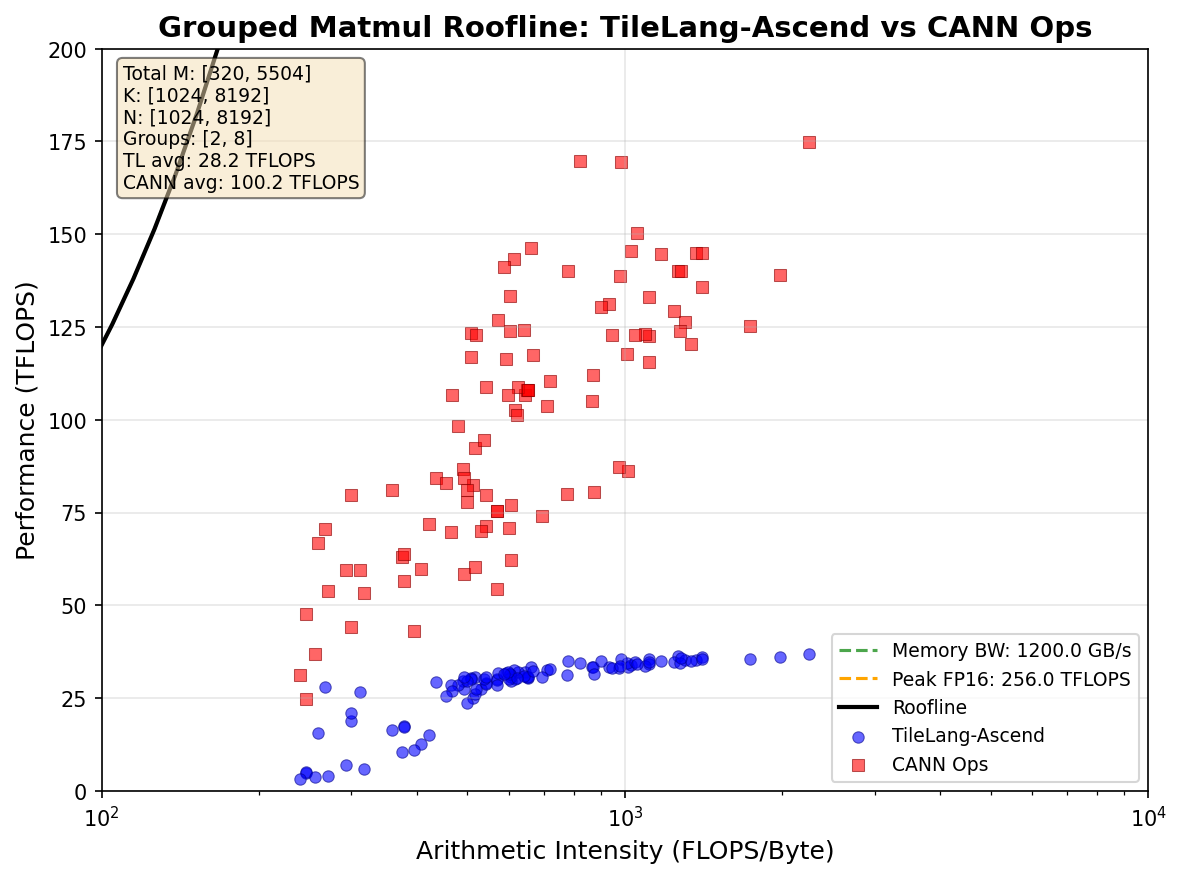
\includegraphics[width=\linewidth]{response_letter/figures/tilelang-vs-cann-gmm.png}
  \end{minipage}\hfill
  \begin{minipage}[t]{0.49\linewidth}
    \centering
    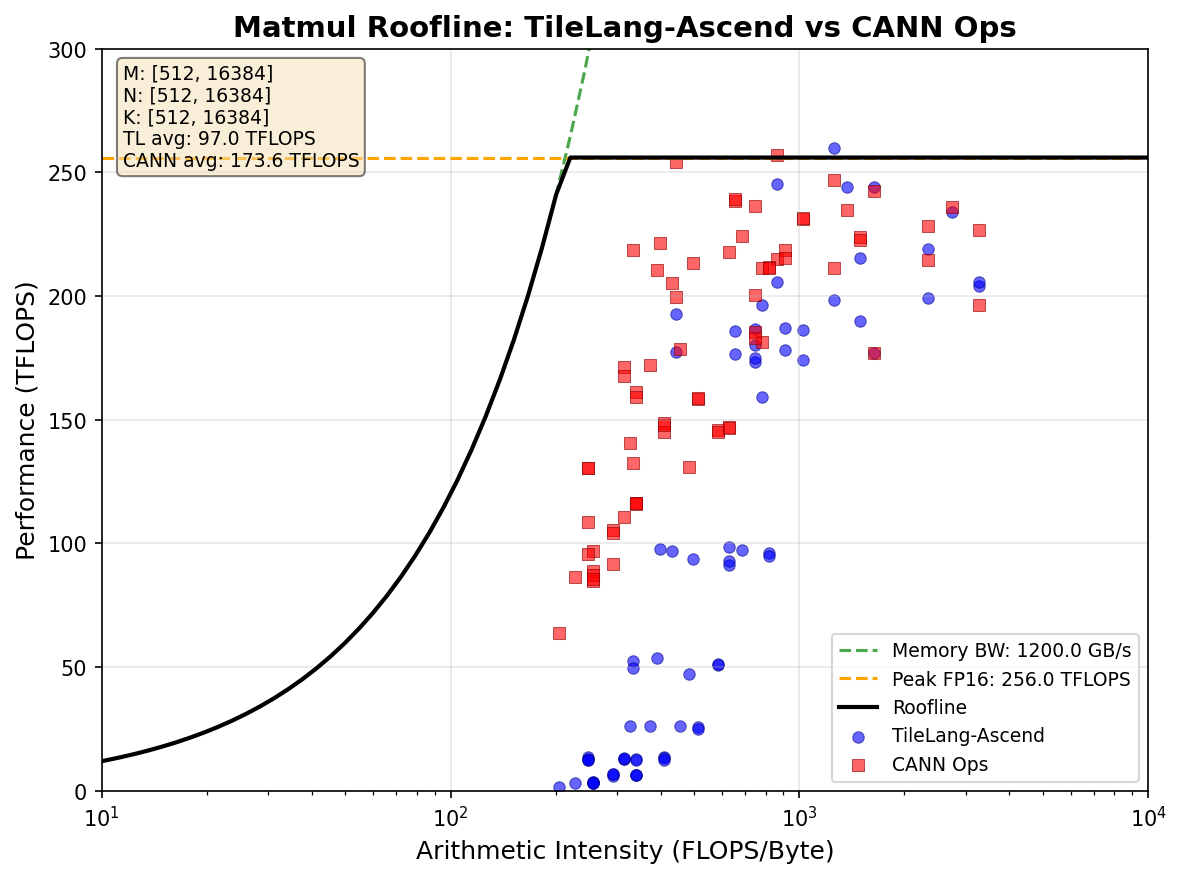
\includegraphics[width=\linewidth]{response_letter/figures/tilelang-vs-cann-mm.png}
  \end{minipage}
  \caption{Ascend roofline characterization of CANN and TileLang-Ascend for
  Grouped Matmul (left) and Matmul (right).}
  \Description{Two Ascend roofline scatter plots comparing TileLang-Ascend and
  CANN for Grouped Matmul and Matmul across sampled arithmetic intensities.}
  \label{fig:tilelang-cann-roofline}
  \vspace{-4pt}
\end{figure}

\loc{\SIntro; \SRelated; \SDiscussion.  The roofline plots above are included only in this
response and were not added to the manuscript.}

\reviewcomment{R3.3: NPU and GPU compilation paths}{resp:r3-3}
{The design should explain compilation and instruction translation for the
two accelerators.}

\authorresponse
TilingInfer operates within the compilation flow of existing expert-written
libraries.  It analyzes and transforms LLVM IR emitted from their C++ host and
device implementations, but it does not modify the subsequent
backend-specific lowering from compiler IR to GPU or NPU machine instructions.
The existing accelerator backend and instruction-selection pipelines remain
unchanged.

Because backend instruction lowering is outside TilingInfer's optimization
scope and is not required to explain its cross-layer constant propagation, we
did not add backend-lowering details to the manuscript.

\loc{No corresponding manuscript location; response clarification only.}

\reviewcomment{R3.4: Is the cross-language gap a real challenge?}{resp:r3-4}
{Determining tensor shapes and attributes may appear to be a collection of
independent size-specific optimizations followed by simple integration.}

\authorresponse
Thank you for identifying the ambiguity.  Inferring tensor shapes and operator
attributes is not itself a contribution of this work; systems such as Dynamo
and TVM Relax already provide symbolic shape inference.  The challenge is to
materialize the constants and symbolic information available in Graph IR into
an entry state that C++/LLVM analysis can use.

Runtime FFI can pass concrete tensor-shape and operator-attribute values, but it
does not preserve the distinction between constant and symbolic dimensions in
Graph IR as compile-time information usable by a separately compiled operator
library.  After entering C++, parameters such as Tensor, List, and Optional are
represented as composite objects with nested memory layouts, and their accesses
are lowered to pointer arithmetic and field loads.  End-to-end cross-language
static analysis would also need to process framework dispatch, type conversion,
object construction, value copying, reference counting, and other FFI code
unrelated to the target mapping, making the analysis expensive and
framework-specific.

TilingInfer defines type-directed context-update rules for the five core
parameter types Scalar, String, Tensor, List, and Optional.  These rules
directly materialize Graph IR metadata as abstract states at the corresponding
C++ object fields and memory locations, while recursive rules support standard
nested compositions.  The rules are selected by parameter type rather than
concrete size: TilingInfer neither enumerates shapes nor implements separate
optimizations for different sizes, but instead propagates the recovered
constants through the same C++/LLVM implementation to kernel launch sites.

Therefore, this process is neither simple parameter passing nor a collection
of independent size-specific optimizations.

\loc{\SIntro; \papersec{sec:motivation:challenges},
``Challenges and Design Insights.''}

\reviewcomment{R3.5: Meaning of the rules
\texorpdfstring{$\mathcal{R}$}{R}}{resp:r3-5}
{What do the rules in Fig.~8 represent, and are they optimizations for
different operator sizes?}

\authorresponse
These rules are neither tiling rules nor size-selection rules.  They are
mappings from Graph IR to C++ memory objects for five basic operator parameter
types: Scalar, String, Tensor, List, and Optional.  For the metadata of a given
Graph IR node, the rules define how to construct the C++ entry state.

To avoid reader confusion, we revised the workflow text and title in Fig.~8,
introduced the meaning of the rule family $\mathcal{R}$ at the beginning of
Section~3.2, and listed the symbol for each rule in Table~2 so that the role of
$\mathcal{R}$ is explicit.

\loc{\papersec{sec:design:context_construction}, especially
\paperfig{fig:context_workflow} and \papertab{tab:semantic-rules}.}

\enlargethispage{3\baselineskip}
\noindent Sincerely,\\
on behalf of all authors


% Start the appended marked manuscript with fresh counters and restore the
% paper's original hyperlink namespaces.
\clearpage
\hypersetup{pageanchor=false}
\pagenumbering{arabic}
\setcounter{section}{0}
\setcounter{subsection}{0}
\setcounter{subsubsection}{0}
\setcounter{paragraph}{0}
\setcounter{figure}{0}
\setcounter{table}{0}
\setcounter{equation}{0}
\setcounter{footnote}{0}
\makeatletter
\@ifundefined{c@algorithm}{}{\setcounter{algorithm}{0}}
\@ifundefined{c@definition}{}{\setcounter{definition}{0}}
\@ifundefined{c@lstlisting}{}{\setcounter{lstlisting}{0}}
\global\ACM@linecount\@ne
\makeatother
\let\theHsection\PaperHSection
\let\theHsubsection\PaperHSubsection
\let\theHsubsubsection\PaperHSubsubsection
\let\theHfigure\PaperHFigure
\let\theHtable\PaperHTable
\let\theHequation\PaperHEquation
\pagestyle{standardpagestyle}
\hypersetup{pageanchor=true}

%%
%% The "title" command has an optional parameter,
%% allowing the author to define a "short title" to be used in page headers.
\title{Optimizing Dynamic-Shape Operator Libraries via Automatic \DIFdelbegin \DIFdel{Kernel }\DIFdelend \DIFaddbegin \DIFadd{Model-Specific }\DIFaddend Specialization on AI Accelerators}

%%
%% The "author" command and its associated commands are used to define
%% the authors and their affiliations.
%% Of note is the shared affiliation of the first two authors, and the
%% "authornote" and "authornotemark" commands
%% used to denote shared contribution to the research.
% \author{Shuo Liu}
% \authornote{Both authors contributed equally to this research.}
% \email{zkdliushuo@mail.ustc.edu.cn}
% \orcid{1234-5678-9012}
% \affiliation{%
%   \institution{University of Science and Technology of China}
%   \city{Hefei}
%   \state{Anhui}
%   \country{CN}
% }

% \author{Lars Th{\o}rv{\"a}ld}
% \affiliation{%
%   \institution{The Th{\o}rv{\"a}ld Group}
%   \city{Hekla}
%   \country{Iceland}}
% \email{larst@affiliation.org}

%%
%% By default, the full list of authors will be used in the page
%% headers. Often, this list is too long, and will overlap
%% other information printed in the page headers. This command allows
%% the author to define a more concise list
%% of authors' names for this purpose.
% \renewcommand{\shortauthors}{Shuo et al.}

\begin{abstract}
{\color{red}%
\DIFdel{%
Deep learning (DL) frameworks rely heavily on operator libraries to support diverse model architectures and dynamic input shapes. To maintain flexibility, these libraries employ generic kernels with numerous runtime parameters for optimal scheduling. However, relying on runtime resolution for these parameters hurts performance, whereas statically enumerating them for efficiency leads to severe code bloat, creating a fundamental dilemma: accepting performance degradation with generic kernels or suffering severe code bloat through exhaustive specialization.
}
\par}
{\color{blue}%
Deep-learning (DL) systems rely on expert-written operator libraries for high performance across dynamic input shapes. These libraries use shape-dependent schedule parameters, such as tile sizes and on-chip buffer layouts. Schedule-generic expert-written operator libraries preserve shape coverage with a single kernel but limit compile-time optimization, whereas schedule-fixed expert-written operator libraries precompile combinations of schedule parameters and incur binary bloat. Kernel-generation compilers do not resolve this trade-off because they generate new kernels rather than specialize existing libraries.
\par}

{\color{red}%
\DIFdel{%
A promising solution is to specialize kernels by propagating model-specific constants from the framework to the compiler. However, this approach faces two challenges: (1) Cross-language semantic gap, where constant information in the high-level Python DSL fails to propagate to device-native C++ compilers, and (2) Control flow obstruction, where extensive validity checks on dynamic dimensions generate massive execution paths handling invalid shapes, thereby impeding the precision and efficiency of constant propagation.
}
\par}
{\color{blue}%
Although many schedule parameters are fixed for a given model, the corresponding model-specific constants recorded in Graph IR are absent from the LLVM IR of separately compiled C++ operator libraries. Runtime argument transmission through Python/C++ FFI does not make these values available as compile-time facts. Propagating model-specific constants from the framework enables specialization, but existing toolchains face two challenges: the Python/C++ semantic gap prevents constant information from reaching the native compiler, and shape checkers for dynamic dimensions introduce many early-exit paths that weaken constant propagation.
\par}

{\color{red}%
\DIFdel{%
We present TilingInfer, the first framework designed to automate kernel specialization in cross-language and dynamic-shape scenarios. To bridge the semantic gap, TilingInfer employs program synthesis to generate partial evaluation programs directly from the Graph IR. To handle control flow, it constructs a Conditional Return-Value Flow Graph to trace the relationship between shape check conditions and early-exit paths, enabling efficient identification and pruning of infeasible execution paths through lightweight constant comparison.
}
\par}
{\color{blue}%
We present TilingInfer, a static-analysis framework that uses LLVM to propagate Graph IR shape information through existing C++ operator libraries and derive constant schedule parameters for kernel specialization and redundant-code elimination. To address the two challenges above, TilingInfer introduces two core designs. First, type-specific context-update rules construct C++ entry states directly from Graph IR shapes and attributes, avoiding analysis of Python/C++ FFI glue code. Second, a Conditional Return-Value Flow Graph identifies early-exit paths and prevents their states from affecting normal paths, preserving precision without analyzing every path.
\par}

{\color{red}%
\DIFdel{%
We implement TilingInfer on Ascend NPUs and NVIDIA GPUs. Evaluations on state-of-the-art libraries (CANN and FlashInfer) demonstrate its effectiveness: TilingInfer achieves an average 1.06$\times$ speedup (up to 1.17$\times$) on Ascend operators and 1.03$\times$ speedup on LLM inference. Furthermore, it reduces the binary size of FlashInfer by over 96\% on GPUs, demonstrating significant potential for library slimming.
}
\par}
{\color{blue}%
On an Ascend NPU, Tiling achieves an average $1.06\times$ operator speedup across diverse operators and an average $1.05\times$ speedup across six representative inference scenarios. It provides larger benefits in the LLM decode phase and recommendation models, averaging a $1.10\times$ speedup. On an NVIDIA GPU, it reduces a 542\,MB binary size by 88.8--95.5\% across 17 model variants.
\par}
\end{abstract}



%%
%% The code below is generated by the tool at http://dl.acm.org/ccs.cfm.
%% Please copy and paste the code instead of the example below.
\begin{CCSXML}
	<ccs2012>
	<concept>
		<concept_id>10011007.10011006.10011041.10011045</concept_id>
		<concept_desc>Software and its engineering~Dynamic compilers</concept_desc>
		<concept_significance>500</concept_significance>
		</concept>
	<concept>
		<concept_id>10010520.10010521.10010528.10010534</concept_id>
		<concept_desc>Computer systems organization~Single instruction, multiple data</concept_desc>
		<concept_significance>300</concept_significance>
		</concept>
	<concept>
		<concept_id>10010147.10010257.10010293.10010294</concept_id>
		<concept_desc>Computing methodologies~Neural networks</concept_desc>
		<concept_significance>300</concept_significance>
		</concept>
	<concept>
		<concept_id>10002944.10011123.10011674</concept_id>
		<concept_desc>General and reference~Performance</concept_desc>
		<concept_significance>300</concept_significance>
		</concept>
	</ccs2012>
\end{CCSXML}

\ccsdesc[500]{Software and its engineering~Dynamic compilers}
\ccsdesc[300]{Computer systems organization~Single instruction, multiple data}
\ccsdesc[300]{Computing methodologies~Neural networks}
\ccsdesc[300]{General and reference~Performance}

\keywords{compilers, static analysis, deep learning, kernel specialization, constant propagation, AI accelerators, operator libraries}

% \received{20 February 2007}
% \received[revised]{12 March 2009}
% \received[accepted]{5 June 2009}

%%
%% This command processes the author and affiliation and title
%% information and builds the first part of the formatted document.
\let\CombinedDocumentRef\ref
\def\PaperTotPagesLabel{TotPages}
\def\ref#1{%
  \def\CurrentReferenceLabel{#1}%
  \ifx\CurrentReferenceLabel\PaperTotPagesLabel
    \PaperTotPagesLink
  \else
    \CombinedDocumentRef{#1}%
  \fi}
\maketitle
\let\ref\CombinedDocumentRef

\section{Introduction}\label{sec:intro}

{\color{red}%
\DIFdel{%
DL frameworks and serving systems~}\mbox{\cite{ansel2024dynamo,abadi2016tensorflow,kwon2023vllm,zheng2024sglang}}\hspace{0pt}\DIFdel{ rely heavily on hand-written operator libraries~}\mbox{\cite{nvidia2021cublas,nvidia2017cutlass,ye2025flashinfer,ascend_cannopsadv,dao2024flashattention2,flashmla2025}}\hspace{0pt}\DIFdel{ to ensure efficient operator implementation. To achieve universal applicability, these libraries must handle input dynamics arising from two main sources: (1) Cross-model heterogeneity, involving diverse algorithmic variants (e.g., attention mechanisms~}\mbox{\cite{vaswani2017attention,ainslie2023gqa,shazeer2019fast,beltagy2020longformerlongdocumenttransformer}}\hspace{0pt}\DIFdel{) and varying attributes (e.g., head numbers~}\mbox{\cite{yang2024qwen2technicalreport,touvron2023llama2openfoundation,deepseekai2025deepseekv3technicalreport}}\hspace{0pt}\DIFdel{); and (2) Input shape variability, where dimensions like batch sizes and sequence lengths vary at runtime.
}
\par}
{\color{blue}%
Deep-learning (DL) frameworks and serving systems~\cite{ansel2024dynamo,abadi2016tensorflow,kwon2023vllm,zheng2024sglang} rely heavily on expert-written operator libraries~\cite{nvidia2021cublas,nvidia2017cutlass,ye2025flashinfer,ascend_cannopsadv,dao2024flashattention2,flashmla2025}. These libraries must cover input dynamics from both cross-model heterogeneity (such as different algorithmic variants~\cite{vaswani2017attention,ainslie2023gqa,shazeer2019fast,beltagy2020longformerlongdocumenttransformer} and architectural attributes~\cite{yang2024qwen2technicalreport,touvron2023llama2openfoundation,deepseekai2025deepseekv3technicalreport}) and runtime variation in dimensions (such as batch size and sequence length). The performance of each resulting operator configuration depends not only on its algorithm but also on its \emph{schedule parameters}, including tile sizes, loop bounds, pipeline stages, and memory layout choices. Different shapes can have different optimal schedules. Consequently, when input shapes are dynamic, the operator implementation must select a high-performance schedule based on the runtime shape.
\par}

{\color{red}%
\DIFdel{%
Existing operator libraries adopt different specialization strategies depending on the underlying hardware characteristics, yet both approaches face critical limitations as illustrated in }\autoref{fig:comparison-libraries}\DIFdel{.
}
\par}
{\color{blue}%
Existing approaches can be classified by how their generated binaries represent schedule parameters. A \emph{schedule-fixed kernel} compiles the key schedule parameters as constants, so each compiled kernel realizes a fixed schedule. A \emph{schedule-generic kernel} retains the schedule parameters as runtime variables, allowing one compiled kernel to realize different schedules for different shapes. The four approaches in \autoref{fig:comparison-libraries} comprise three schedule-fixed approaches (\ding{172}--\ding{174}) and one schedule-generic approach (\ding{175}).
\par}

\begin{figure*}[t]
    \centering
    \vspace{-6pt}

    % OpenTikZ light palette. All figure colors are referenced by these
    % semantic palette names so the artwork remains easy to retheme.
    \definecolor{otblue}{HTML}{1F5AA9}
    \definecolor{otorange}{HTML}{A66A00}
    \definecolor{otteal}{HTML}{3D7B2A}
    \definecolor{otpurple}{HTML}{7357B8}
    \definecolor{otgray}{HTML}{111111}

    % Parametric geometry for the two-by-two comparison and its legend.
    \def\KernelColumnShift{8.15cm}
    \def\KernelRowShift{-5.12cm}
    \def\KernelPhaseWidth{4.86cm}
    \def\KernelBinaryWidth{2.50cm}
    \def\KernelRowGap{0.75cm}
    \def\LegendCellPitch{2.67}

    \resizebox{\textwidth}{!}{%
    \begin{tikzpicture}[
        font=\fontfamily{phv}\fontsize{6.5pt}{7.5pt}\selectfont,
        panel number/.style={
            circle,
            draw=otblue,
            fill=otblue,
            text=otgray!0,
            line width=0.8pt,
            minimum size=0.40cm,
            inner sep=0pt,
            font=\fontfamily{phv}\selectfont\normalsize\bfseries,
            drop shadow={
                shadow xshift=0.45pt,
                shadow yshift=-0.45pt,
                opacity=0.16,
                fill=otblue
            }
        },
        panel title/.style={
            anchor=west,
            text=otgray,
            font=\fontfamily{phv}\selectfont\normalsize\bfseries,
            inner sep=0pt
        },
        phase region/.style={
            draw=otblue!72,
            fill=otblue!3,
            rounded corners=2.5pt,
            line width=0.72pt,
            minimum width=\KernelPhaseWidth,
            minimum height=1.93cm
        },
        phase heading/.style={
            text=otblue,
            font=\fontfamily{phv}\selectfont\scriptsize\bfseries,
            inner sep=0pt
        },
        jit phase region/.style={
            phase region,
            draw=otorange!82,
            fill=otorange!8
        },
        jit phase heading/.style={
            phase heading,
            text=otorange!82
        },
        module/.style={
            draw=otgray!78,
            fill=otgray!0,
            rounded corners=1pt,
            line width=0.56pt,
            minimum height=0.48cm,
            inner xsep=5pt,
            inner ysep=3pt,
            align=center,
            text=otgray,
            drop shadow={
                shadow xshift=0.35pt,
                shadow yshift=-0.35pt,
                opacity=0.10,
                fill=otgray
            }
        },
        input module/.style={
            module,
            draw=otpurple!72,
            fill=otpurple!8,
            minimum width=1.92cm
        },
        compile module/.style={
            module,
            draw=otorange!82,
            fill=otorange!8,
            minimum width=1.62cm
        },
        runtime module/.style={
            module,
            draw=otorange!82,
            fill=otorange!8,
            minimum width=1.70cm,
            font=\fontfamily{phv}\selectfont\scriptsize\bfseries
        },
        binary region/.style={
            draw=otteal!78,
            fill=otteal!2,
            densely dashed,
            rounded corners=2.5pt,
            line width=0.72pt,
            minimum width=\KernelBinaryWidth,
            minimum height=2.12cm
        },
        binary heading/.style={
            text=otteal!72!otgray,
            font=\fontfamily{phv}\fontsize{7.5pt}{8.2pt}\selectfont\bfseries,
            inner sep=0pt
        },
        binary class label/.style={
            text=otgray,
            font=\fontfamily{phv}\fontsize{6.1pt}{6.8pt}\selectfont,
            inner sep=0pt,
            align=center
        },
        generates/.style={
            -{Latex[length=2.0mm,width=1.35mm]},
            draw=otblue,
            line width=1.0pt,
            rounded corners=1pt
        },
        data flow/.style={
            -{Latex[length=1.9mm,width=1.35mm]},
            draw=otgray,
            line width=0.78pt
        },
        correspondence/.style={
            draw=otgray,
            densely dashed,
            line width=0.62pt
        },
        dispatch/.style={
            -{Latex[length=1.9mm,width=1.35mm]},
            draw=otgray,
            line width=0.78pt
        },
        internal flow/.style={
            -{Latex[length=1.75mm,width=1.2mm]},
            draw=otgray,
            line width=0.68pt
        },
        divider/.style={
            draw=otgray!23,
            dash pattern=on 1.4pt off 1.7pt,
            line width=0.58pt
        },
        legend label/.style={
            anchor=west,
            text=otgray,
            font=\fontfamily{phv}\fontsize{6.4pt}{7.1pt}\selectfont,
            inner sep=0pt,
            align=left
        }
    ]

    % Quadrant separators and legend rule.
    \draw[divider] (7.98,0.38) -- (7.98,-9.55);
    \draw[divider] (0,-4.64) -- (16.02,-4.64);
    \draw[otblue!25, line width=0.60pt] (0,-9.27) -- (16.02,-9.27);

    % ==================================================================
    % 1. JIT code generation: one compilation for each runtime shape.
    % ==================================================================
    \begin{scope}[xshift=0cm,yshift=0cm]
        \node[panel number] (a-number) at (0.45,0) {1};
        \node[panel title, right=0.22cm of a-number]
              (a-title) {\scalebox{0.88}[1]{%
                  \textbf{JIT Code Generation (Per-Shape Compilation)}}};

        \node[jit phase region, anchor=north west] (a-phase) at (0.24,-0.46) {};
        \node[jit phase heading] (a-phase-heading) at (2.69,-0.74)
              {\textbf{JIT Compile}};
        \node[module, minimum width=2.50cm] (a-static-description)
              at (1.70,-1.26)
              {\scalebox{0.90}[1]{Static Shape Description}};
        \node[module, minimum width=2.50cm] (a-operator-specification)
              at (1.70,-1.88)
              {\scalebox{0.90}[1]{Operator Specification}};
        \node[module, minimum width=1.42cm] (a-autotune)
              at (4.18,-1.57) {AutoTune};
        \draw[internal flow] (a-static-description.east) --
            ($(a-autotune.west)+(0,0.12cm)$);
        \draw[internal flow] (a-operator-specification.east) --
            ($(a-autotune.west)+(0,-0.12cm)$);

        \node[input module] (a-shape-1) at (1.24,-2.99) {Shape $S_1$};
        \node[input module] (a-shape-2)
              at ($(a-shape-1)+(0,-\KernelRowGap)$) {Shape $S_2$};
        \node[compile module] (a-jit-1) at (3.86,-2.99) {JIT Compile};
        \node[compile module] (a-jit-2)
              at ($(a-jit-1)+(0,-\KernelRowGap)$) {JIT Compile};

        \node[binary region, minimum height=2.50cm] (a-binary) at (6.63,-3.13) {};
        \node[binary heading] (a-binary-heading) at (6.63,-2.10)
              {\textbf{Generated Binary}};
        \node[binary class label] (a-binary-class) at (6.63,-2.45)
              {Schedule-Fixed};
        \node[module, minimum width=1.56cm] (a-kernel-1)
              at (a-binary.center |- a-jit-1.center)
              {Kernel 1};
        \node[module, minimum width=1.56cm] (a-kernel-2)
              at (a-binary.center |- a-jit-2.center)
              {Kernel 2};

        \draw[correspondence] (a-jit-1.north west) -- (a-phase.south west);
        \draw[correspondence] (a-jit-1.north east) -- (a-phase.south east);
        \draw[data flow] (a-shape-1) -- (a-jit-1);
        \draw[data flow] (a-shape-2) -- (a-jit-2);
        \draw[data flow] (a-jit-1.east) -- (a-kernel-1.west);
        \draw[data flow] (a-jit-2.east) -- (a-kernel-2.west);
        \coordinate (a-binary-entry) at ($(a-binary.north)+(-0.09cm,0)$);
        \draw[generates] (a-autotune.east) --
            (a-binary-entry |- a-autotune.east) -- (a-binary-entry);
    \end{scope}

    % ==================================================================
    % 2. AOT code generation: emit kernels and a runtime dispatcher.
    % ==================================================================
    \begin{scope}[xshift=\KernelColumnShift,yshift=0cm]
        \node[panel number] (b-number) at (0.39,0) {2};
        \node[panel title, right=0.12cm of b-number]
              (b-title) {\scalebox{1.05}[1]{%
                  \textbf{AOT Code Generation with Runtime Dispatch}}};

        \node[phase region, anchor=north west, minimum width=5.12cm]
              (b-phase) at (0.18,-0.46) {};
        \node[phase heading] (b-phase-heading) at (2.74,-0.74)
              {\textbf{AOT Compile}};
        \node[module, minimum width=2.72cm] (b-dynamic-description)
              at (1.69,-1.26)
              {\scalebox{0.84}[1]{Dynamic Shape Description}};
        \node[module, minimum width=2.72cm] (b-operator-specification)
              at (1.69,-1.88)
              {\scalebox{0.90}[1]{Operator Specification}};
        \node[module, minimum width=1.44cm] (b-autotune)
              at (4.40,-1.57) {AutoTune};
        \draw[internal flow] (b-dynamic-description.east) --
            ($(b-autotune.west)+(0,0.12cm)$);
        \draw[internal flow] (b-operator-specification.east) --
            ($(b-autotune.west)+(0,-0.12cm)$);

        \node[input module] (b-shape-1) at (1.17,-3.18) {Shape $S_1$};
        \node[input module] (b-shape-2) at (1.17,-3.91) {Shape $S_2$};
        \node[runtime module, minimum width=1.68cm, minimum height=1.10cm]
              (b-dispatcher) at (3.76,-3.55)
              {\textbf{Generated}\\\textbf{Dispatcher}};

        \node[binary region, minimum height=2.50cm] (b-binary) at (6.60,-3.23) {};
        \node[binary heading] (b-binary-heading) at (6.60,-2.19)
              {\textbf{Generated Binary}};
        \node[binary class label] (b-binary-class) at (6.60,-2.54)
              {Schedule-Fixed};
        \node[module, minimum width=1.56cm] (b-kernel-1)
              at (b-binary.center |- b-shape-1.center)
              {Kernel 1};
        \node[module, minimum width=1.56cm] (b-kernel-2)
              at (b-binary.center |- b-shape-2.center)
              {Kernel 2};

        \draw[data flow] (b-shape-1.east) --
            (b-dispatcher.west |- b-shape-1.east);
        \draw[data flow] (b-shape-2.east) --
            (b-dispatcher.west |- b-shape-2.east);
        \draw[dispatch] (b-dispatcher.east |- b-kernel-1.west) --
            (b-kernel-1.west);
        \draw[dispatch] (b-dispatcher.east |- b-kernel-2.west) --
            (b-kernel-2.west);
        \coordinate (b-binary-entry) at ($(b-binary.north)+(-0.05cm,0)$);
        \draw[generates] (b-autotune.east) --
            (b-binary-entry |- b-autotune.east) -- (b-binary-entry);
        \coordinate (b-dispatcher-generation-bend)
              at ($(b-autotune.south)+(0,-0.75cm)$);
        \draw[generates] (b-autotune.south) --
            (b-dispatcher-generation-bend) -| (b-dispatcher.north);
    \end{scope}

    % ==================================================================
    % 3. AOT compilation with enumerated template parameters.
    % ==================================================================
    \begin{scope}[xshift=0cm,yshift=\KernelRowShift]
        \node[panel number] (c-number) at (0.38,0) {3};
        \node[panel title, right=0.22cm of c-number]
              (c-title) {\scalebox{0.82}[1]{%
                  \textbf{AOT Compile with Enumerated Templates}}};

        \node[phase region, anchor=north west, minimum width=5.16cm,
              minimum height=1.52cm] (c-phase) at (0.17,-0.46) {};
        \node[phase heading] (c-phase-heading) at (2.77,-0.79)
              {\textbf{AOT Compile}};
        \node[module, minimum width=1.97cm] (c-template-source)
              at (1.33,-1.33) {Template Kernel\\Source Code};
        \node[module, minimum width=2.16cm] (c-enumerate)
              at (4.07,-1.33)
              {\scalebox{0.88}[1]{Enumerate Template}\\Parameters};
        \draw[internal flow] (c-template-source) -- (c-enumerate);

        \node[input module] (c-shape-1) at (1.19,-2.71) {Shape $S_1$};
        \node[input module] (c-shape-2) at (1.19,-3.38) {Shape $S_2$};
        \node[runtime module, minimum width=1.72cm, minimum height=1.10cm]
              (c-dispatcher) at (3.80,-3.06)
              {\textbf{Expert-Written}\\\textbf{Dispatcher}};

        \node[binary region, minimum height=2.50cm]
              (c-binary) at (6.63,-2.80) {};
        \node[binary heading] (c-binary-heading) at (6.63,-1.78)
              {\textbf{Generated Binary}};
        \node[binary class label] (c-binary-class) at (6.63,-2.13)
              {Schedule-Fixed};
        \node[module, minimum width=1.56cm] (c-kernel-1)
              at (c-binary.center |- c-shape-1.center)
              {Kernel 1};
        \node[module, minimum width=1.56cm] (c-kernel-2)
              at (c-binary.center |- c-shape-2.center)
              {Kernel 2};

        \draw[data flow] (c-shape-1.east) --
            (c-dispatcher.west |- c-shape-1.east);
        \draw[data flow] (c-shape-2.east) --
            (c-dispatcher.west |- c-shape-2.east);
        \draw[dispatch] (c-dispatcher.east |- c-kernel-1.west) --
            (c-kernel-1.west);
        \draw[dispatch] (c-dispatcher.east |- c-kernel-2.west) --
            (c-kernel-2.west);
        \draw[generates] (c-enumerate.east) --
            (c-binary.north |- c-enumerate.east) -- (c-binary.north);
    \end{scope}

    % ==================================================================
    % 4. AOT compilation of one schedule-generic kernel with runtime scheduling.
    % ==================================================================
    \begin{scope}[xshift=\KernelColumnShift,yshift=\KernelRowShift]
        \node[panel number] (d-number) at (0.38,0) {4};
        \node[panel title, right=0.14cm of d-number]
              (d-title) {\scalebox{0.94}[1]{%
                  \textbf{AOT Compile with Schedule-Generic Kernel}}};

        \node[phase region, anchor=north west, minimum width=2.98cm,
              minimum height=1.57cm] (d-phase) at (0.18,-0.46) {};
        \node[phase heading] (d-phase-heading) at (1.69,-0.79)
              {\textbf{AOT Compile}};
        \node[module, minimum width=2.60cm] (d-generic-source)
              at (1.69,-1.40) {Schedule-Generic\\Kernel Source Code};

        \node[input module] (d-shape-1) at (1.10,-2.72) {Shape $S_1$};
        \node[input module] (d-shape-2) at (1.10,-3.32) {Shape $S_2$};
        \node[runtime module, minimum width=1.72cm, minimum height=1.10cm]
              (d-scheduler) at (3.76,-3.01)
              {\textbf{Expert-Written}\\\textbf{Scheduler}};

        \node[binary region, minimum height=2.00cm] (d-binary)
              at (6.60,-2.67) {};
        \node[binary heading] (d-binary-heading) at (6.60,-1.92)
              {\textbf{Generated Binary}};
        \node[binary class label] (d-binary-class) at (6.60,-2.27)
              {Schedule-Generic};
        \node[module, minimum width=1.48cm] (d-generic-kernel)
              at (d-binary.center |- d-scheduler.center) {Schedule-Generic\\Kernel};

        \draw[data flow] (d-shape-1.east) --
            (d-scheduler.west |- d-shape-1.east);
        \draw[data flow] (d-shape-2.east) --
            (d-scheduler.west |- d-shape-2.east);
        \draw[dispatch] (d-scheduler.east) -- (d-generic-kernel.west);
        \coordinate (d-binary-entry) at ($(d-binary.north)+(-0.10cm,0)$);
        \draw[generates] (d-generic-source.east) --
            (d-binary-entry |- d-generic-source.east) -- (d-binary-entry);
    \end{scope}

    % ==================================================================
    % Legend: visual semantics used consistently by all four panels.
    % ==================================================================
    \foreach \legendindex in {0,...,5} {
        \coordinate (legend-slot-\legendindex)
            at ({0.13+\legendindex*\LegendCellPitch},-9.75);
    }

    \node[input module, minimum width=0.54cm, minimum height=0.34cm,
          inner sep=0pt] (legend-input)
          at ($(legend-slot-0)+(0.47,0)$) {};
    \node[legend label, right=0.15cm of legend-input]
          {Input (Runtime)};

    \node[phase region, minimum width=0.54cm, minimum height=0.34cm,
          inner sep=0pt] (legend-aot-compile)
          at ($(legend-slot-1)+(0.67,0)$) {};
    \node[legend label, right=0.15cm of legend-aot-compile]
          {AOT Compile};

    \node[binary region, minimum width=0.54cm, minimum height=0.34cm,
          inner sep=0pt] (legend-binary)
          at ($(legend-slot-2)+(0.27,0)$) {};
    \node[legend label, right=0.15cm of legend-binary]
          {Compilation Output\\(Generated Binary)};

    \node[runtime module, minimum width=0.54cm, minimum height=0.34cm,
          inner sep=0pt] (legend-runtime)
          at ($(legend-slot-3)+(0.27,0)$) {};
    \node[legend label, right=0.15cm of legend-runtime]
          {Runtime Component};

    \draw[dispatch] ($(legend-slot-4)+(0.46,0)$) --
        ($(legend-slot-4)+(1.02,0)$);
    \node[legend label] at ($(legend-slot-4)+(1.18,0)$)
          {Data Flow \&\\Launch Kernel};

    \draw[generates] ($(legend-slot-5)+(0.15,0)$) --
        ($(legend-slot-5)+(0.71,0)$);
    \node[legend label] at ($(legend-slot-5)+(0.87,0)$)
          {Code Generation};

    % Preserve the same lower whitespace visible in the reference artwork.
    \path (0,-10.18) coordinate (figure-bottom-padding);

    \end{tikzpicture}%
    }

    \caption{Four ways to compile and execute dynamic-shape operators.}
    \Description{A color-coded two-by-two TikZ comparison. Each panel shows two purple runtime shape inputs. The green dashed generated-binary containers in panels 1--3 are labeled Schedule-Fixed, while the container in panel 4 is labeled Schedule-Generic. Light-blue regions are AOT compilation stages, and orange boxes are JIT compilation or runtime components. Blue arrows denote code generation, solid black arrows denote data flow and kernel launch, and black dashed lines associate the first per-shape JIT compilation with the shared JIT compilation stage.}
    \label{fig:comparison-libraries}
    \vspace{-8pt}
\end{figure*}


{\color{red}%
\DIFdel{%
Meanwhile, although AI compilers~}\mbox{\cite{tillet2019triton,chen2018tvm,zheng2022dietcode,shen2021nimble,zheng2023bladedisc}}\hspace{0pt}\DIFdel{ offer an alternative by generating specialized kernels at runtime, they are typically confined to specific high-level IRs (e.g., Triton IR~}\mbox{\cite{tillet2019triton}}\hspace{0pt}\DIFdel{ and Relax~}\mbox{\cite{Lai2023RelaxCA}}\hspace{0pt}\DIFdel{) and incur non-negligible runtime compilation overhead.
}
\par}
{\color{blue}%
AI compilers produce schedule-fixed kernels through schedule search and code generation. \ding{172}~A static-shape AI compiler takes a concrete shape as input, searches for or autotunes a schedule for that shape, and generates a shape-specific kernel, often through a just-in-time (JIT) compilation path~\cite{chen2018autotvm,zheng2020ansor,tilelang,tillet2019triton}. An unseen shape triggers another round of schedule search and code generation. \ding{173}~A dynamic-shape AI compiler instead searches for schedules over a declared shape range ahead of time. It generates a set of optimized, schedule-fixed kernels together with a dispatcher that maps each runtime shape in the range to an appropriate kernel~\cite{zheng2022dietcode,shen2021nimble,zheng2023bladedisc,Lai2023RelaxCA}.
\par}

{\color{red}%
\DIFdel{%
On GPU platforms, which are highly sensitive to compiler optimizations like loop unrolling, developers usually resort to manual specialization using C++ templates~}\mbox{\cite{nvidia2017cutlass,ye2025flashinfer,dao2024flashattention2}}\hspace{0pt}\DIFdel{ (depicted as \ding{182}). Conversely, on architectures like Ascend~}\mbox{\cite{liao2019davinci}}\hspace{0pt}\DIFdel{ that provide diverse programmable units, the schedule parameters are substantially more numerous. Since manually specializing for such a vast search space is intractable, the vendor libraries (e.g., CANN~}\mbox{\cite{ascend_cannopsadv}}\hspace{0pt}\DIFdel{) on such platforms primarily invoke generic kernels (depicted as \ding{183}), resulting in performance loss due to weakened compiler optimizations.
}
\par}
{\color{blue}%
Expert-written operator libraries implement the other two approaches. \ding{174}~A schedule-fixed expert-written operator library encodes schedule parameters as C++ template parameters and enumerates their candidate values during ahead-of-time (AOT) compilation~\cite{nvidia2017cutlass,ye2025flashinfer,dao2024flashattention2}. This process produces a set of schedule-fixed kernels, from which an expert-written dispatcher selects a template instance for each runtime shape. \ding{175}~A schedule-generic expert-written operator library instead AOT-compiles a schedule-generic kernel. At runtime, an expert-written host-side scheduler applies heuristic rules to the input shape, computes the schedule parameters, and passes them to the device kernel as runtime arguments.
\par}

{\color{red}%
\DIFdel{%
Given these limitations, we focus on hand-written operator libraries and aim to address the shortcomings of both manual specialization and generic kernel approaches: achieving automatic specialization for generic libraries to recover performance loss, and pruning manually specialized libraries to mitigate combinatorial explosion and code bloat.
}
\par}
{\color{blue}%
AI compilers such as Triton and TileLang complement expert-written operator libraries but operate on a different compilation path~\cite{tillet2019triton,tilelang}. These code-generation workflows integrate specialization into the multi-level lowering of a high-level operator program. During lowering, the shape and schedule values selected for specialization are materialized and propagated as constants in the intermediate representations. This process generates a new specialized kernel implementation but does not directly specialize the existing C++/LLVM implementation of an expert-written operator library.
\par}

{\color{red}%
\DIFdel{%
To accommodate such dynamics, operator libraries typically adopt a generic implementation strategy: they calculate schedule parameters (configuration values such as tiling sizes and loop bounds) at runtime on the host side and pass them to the kernel function as variable arguments. However, this generic design comes at a cost. From the perspective of the underlying device native compiler, these critical configuration values appear as unknown variables rather than compile-time constants. This ambiguity effectively weakens aggressive compiler optimizations that rely on static information, such as constant folding, loop unrolling, and instruction schedule. Consequently, this often leads to suboptimal performance. In this context, specializing kernels by replacing input schedule parameters with constants at compile time is generally beneficial, as it can enhance subsequent compiler optimizations. As the complexity of operators~}\mbox{\cite{dao2024flashattention2,ye2025flashinfer}}\hspace{0pt}\DIFdel{ continues to increase and programmable units~}\mbox{\cite{liao2019davinci,jouppi2023tpu}}\hspace{0pt}\DIFdel{ within hardware become increasingly diverse, the number of schedule parameters of kernels explodes, further necessitating kernel specialization. While manual specialization resolves schedule parameters at compile time, exhaustively enumerating parameter combinations to accommodate input dynamics leads to combinatorial explosion and severe code bloat.
}
\par}
{\color{blue}%
The two expert-written library designs expose a common \emph{specialization trade-off}. Schedule-fixed kernels expose schedule parameters as compile-time constants, enabling optimizations such as constant folding, loop unrolling, and instruction scheduling; however, enumerating combinations of schedule parameters causes combinatorial code-size growth. Schedule-generic kernels use a compact binary to cover a large shape space, but representing schedule parameters as runtime variables limits the same compiler optimizations and can reduce performance. This trade-off becomes more pronounced as operator implementations grow more complex~\cite{dao2024flashattention2,ye2025flashinfer} and accelerator architectures expose increasingly diverse programmable units~\cite{liao2019davinci,jouppi2023tpu}. Both trends increase the number of schedule parameters and the size of their configuration space, further exacerbating the trade-off.
\par}

{\color{red}%
\DIFdel{%
To address these limitations, we observe that deploying a specific model exhibits partial dynamics: while input dimensions (e.g., batch size, sequence length) vary at runtime, model-specific attributes (e.g., hidden size, head number) remain invariant throughout serving. We denote these compile-time constants as model-specific constants, which can be resolved by symbolic shape inference in current DL frameworks~}\mbox{\cite{shen2021nimble,zheng2023bladedisc,Lai2023RelaxCA,ansel2024dynamo}}\hspace{0pt}\DIFdel{. A key insight is that kernel schedule configurations are primarily determined by these model-specific constants. Our analysis (\S}\ref{sec:motivation}\DIFdel{) shows that over 90\% of schedule parameters become deterministic given model-specific constants, enabling static resolution of most dynamic schedule decisions.
}
\par}
{\color{blue}%
Our key observation is that most schedule parameters are runtime invariants once a model is deployed. Most deployment scenarios exhibit \emph{partial dynamics}: only a limited set of dimensions, such as batch size and sequence length, vary at runtime, while model-specific attributes and dimensions, such as hidden size, head count, and head dimension, remain fixed. We refer to these fixed facts as model-specific constants. Current DL frameworks can recover model-specific constants through graph capture and symbolic shape inference~\cite{shen2021nimble,zheng2023bladedisc,Lai2023RelaxCA,ansel2024dynamo}. Mechanistically, model-specific constants determine the core tiling and pipeline structure constrained by on-chip resources and compute units, whereas dynamic dimensions primarily affect the number of executions of these tiles, their parallel partitioning, and tail handling. Consistent with this mechanism, our analysis in \S\ref{sec:motivation} finds that, across the studied operators, about 90\% of schedule parameters are runtime invariants determined by model-specific constants and do not depend on the concrete runtime values of dynamic dimensions.
\par}

{\color{red}%
\DIFdel{%
To address the above challenges, we introduce TilingInfer, the first system designed to enable precise constant propagation across language boundaries for kernel specialization. We construct an automated cross-language and whole-program analysis framework for automatic specialization of generic library kernels and code debloating for manually specialized libraries. By introducing mechanisms specific to DL systems, TilingInfer extends traditional static analysis techniques and consists of four main components: (1) Cross-Language Context Reconstruction (\S}\ref{sec:design:context_construction}\DIFdel{) defines semantic mapping rules from Graph IR parameter types to the typed records in C++ memory, automatically generating partially-evaluated calling contexts without analyzing complex FFI glue code; (2) Early-Exit Edge Identification (\S}\ref{sec:design:early-return}\DIFdel{) tracks the value flow of return values and determines whether a path leads to error status codes based on guard conditions, enabling precise pruning of infeasible edges at control-flow merge points; (3) Inter-Procedural Constant Propagation (\S}\ref{sec:design:propagation}\DIFdel{) performs field-sensitive analysis to propagate constants through complex host-side programs; (4) Kernel Specialization and Library Pruning (\S}\ref{sec:design:specialization}\DIFdel{) performs LLVM IR-level transformations to specialize generic kernels and eliminate redundant template instantiations.
}
\par}
{\color{blue}%
This observation suggests a distinct application strategy for addressing the specialization trade-off: using model-specific constants to specialize existing operator libraries. Inspired by this insight, we present \textbf{\uline{TilingInfer}}, a static-analysis framework for LLVM-based operator libraries. It uses LLVM IR as a common representation of C++ operator libraries. TilingInfer first uses graph-level model constants to \textbf{\uline{infer}} invariant \textbf{\uline{tiling}} data (i.e., schedule parameters) for both schedule-fixed and schedule-generic implementations. For each Graph IR node (i.e., an operator invocation), TilingInfer extracts its arguments, shapes, and attributes to construct the entry state of the corresponding host-side LLVM IR function. This construction covers both concrete and symbolic dimensions. TilingInfer then propagates this constructed state information through the host-side LLVM IR programs to device-kernel launch sites. Finally, for a schedule-generic kernel, TilingInfer employs the inferred launch-site constant schedule parameters to specialize the kernel. For the schedule-fixed implementation, TilingInfer identifies template instances that cannot be reached and removes these instances.
\par}

{\color{red}%
\DIFdel{%
Based on this insight, we propose leveraging the model-specific constants as contextual information to perform whole-program constant propagation. By propagating these model-specific constants through the operator library down to the kernel call sites, we can statically specialize generic kernels or prune redundant instances in manually specialized libraries. However, implementing this strategy faces two critical challenges regarding the precision of static analysis: the cross-language semantic gap and early-exit paths from dynamic shape checks. First, the operator library is typically integrated into the framework via Python/C++ Foreign Function Interface (FFI), which creates a semantic gap between high-level Python objects and low-level C++ memory states. Standard static analysis cannot bridge this gap, as existing tools treat FFI glue code as black boxes, failing to model the deep heap layouts and internal indirections of domain-specific objects (e.g., Tensor's nested size arrays) that are essential for reconstructing precise C++ calling contexts. Second, the host-side programs of operators involve many shape checkers for validiting input shape, introducing numerous early-exit paths that return error status codes when shape constraints are violated. Standard static analysis conservatively merges data flows from these early-exit paths with the normal path, thereby corrupting precise constant information and causing significant precision loss at control-flow merge sites.
}
\par}
{\color{blue}%
Realizing TilingInfer faces two key challenges. \textbf{First}, reconstructing the calling context requires bridging \textbf{a cross-language semantic gap} by mapping graph-level constants and symbolic shape information into the field-sensitive entry state of the corresponding C++ operator. Graph IR records constants and symbolic dimensions as typed shapes and attributes, whereas the separately compiled C++/LLVM code exposes nested object layouts and pointer/field accesses. Bridging this gap through end-to-end cross-language analysis would require traversing framework dispatch, type conversion, object construction, and other Python/FFI machinery, making the analysis costly and framework-specific. TilingInfer instead uses type-specific context-update rules to precisely construct the required C++ entry state directly from Graph IR, avoiding analysis of Python/C++ FFI glue code. \textbf{Second}, operator host code contains many \textbf{shape checkers that create early-exit paths}. These paths handle only invalid inputs: they report errors and bypass the normal computation of schedule parameters. As a result, merging states from early-exit and normal paths can pollute the normal-path state and reduce the precision of constant propagation. Meanwhile, analyzing every possible path separately would be too expensive for a large operator library. TilingInfer therefore uses a Conditional Return-Value Flow Graph (CRVFG) to identify early-exit edges from the conditional flow of status return values before propagation. It excludes states propagated along these edges from normal-path merges. This preserves constants without analyzing every path separately.
\par}

\DIFdel{In summary, the main contributions of this paper are as follows:}\par
{\color{red}
\begin{enumerate}
    \item \DIFdel{We propose TilingInfer, a novel static analysis framework that enables precise constant propagation across the DL framework's language boundary (Python/C++) into the underlying operator libraries.}
    \item \DIFdel{We introduce a cross-language context reconstruction method based on semantic modeling of core DL data types, and a conditional return-value flow analysis for identifying early-exit edges.}
    \item \DIFdel{We implement TilingInfer based on LLVM~\cite{lattner2004llvm} and apply it to PyTorch~\cite{ansel2024dynamo}, with extensibility to other Python-based frameworks and hardware backends.}
    \item \DIFdel{Evaluation demonstrates TilingInfer's effectiveness: for generic operators on Ascend, it achieves an average speedup of \textbf{1.06$\times$} (up to \textbf{1.17$\times$}) and \textbf{3\%} end-to-end inference speedup; for manually specialized libraries on GPU, it removes over \textbf{96\%} of redundant kernels.}
\end{enumerate}
}

\DIFadd{This paper makes four contributions:}\par
{\color{blue}
\begin{enumerate}
    \item We devise a mechanism that propagates graph-level shape information into the C++ compiler pipeline without analyzing FFI glue code. We formalize context-update rules that map Graph IR parameter types to the memory states of their underlying C++ implementations, allowing the mechanism to cover different PyTorch backends.
    \item We propose CRVFG-based early-exit path identification for precise constant-propagation analysis of operator host code while avoiding expensive path-sensitive analysis.
    \item We implement TilingInfer, a prototype system for specializing expert-written operator libraries on GPU and NPU platforms. It applies automatic partial evaluation to schedule-generic kernels to reduce scalar overhead and prunes unreachable template instances from schedule-fixed binaries at compile time to reduce binary size.
    \item On an Ascend NPU, TilingInfer achieves a 1.06$\times$ geometric-mean device-kernel speedup across 14 CANN operators and a 1.05$\times$ geometric-mean end-to-end speedup across six representative inference scenarios; it provides larger benefits in the performance-critical LLM decode phase, averaging a 1.10$\times$ end-to-end speedup across the two decode scenarios. On an NVIDIA GPU, it reduces a 542\,MB FlashInfer archive by 88.8--95.5\% across 17 model variants.
\end{enumerate}
}

\begin{comment}
\section{Introduction}\label{sec:intro}

\DIFaddbegin 

Deep-learning (DL) frameworks and serving systems~\cite{ansel2024dynamo,abadi2016tensorflow,kwon2023vllm,zheng2024sglang} rely heavily on \DIFdelbegin \DIFdel{hand-written }\DIFdelend \DIFaddbegin \DIFadd{expert-written }\DIFaddend operator libraries~\cite{nvidia2021cublas,nvidia2017cutlass,ye2025flashinfer,ascend_cannopsadv,dao2024flashattention2,flashmla2025}\DIFdelbegin \DIFdel{to ensure efficient operator implementation. 
To achieve universal applicability, these libraries must handle }\DIFdelend \DIFaddbegin \DIFadd{. 
These libraries must cover }\DIFaddend input dynamics \DIFdelbegin \DIFdel{arising from two main sources: (1) Cross-model heterogeneity , involving diverse algorithmic variants(e.g., attention mechanisms~\mbox{%DIFAUXCMD
\cite{vaswani2017attention,ainslie2023gqa,shazeer2019fast,beltagy2020longformerlongdocumenttransformer} }\hspace{0pt}%DIFAUXCMD
) and varying attributes(e.g., head numbers}\DIFdelend \DIFaddbegin \DIFadd{from both cross-model heterogeneity (such as different algorithmic variants~\mbox{%DIFAUXCMD
\cite{vaswani2017attention,ainslie2023gqa,shazeer2019fast,beltagy2020longformerlongdocumenttransformer} }\hspace{0pt}%DIFAUXCMD
and architectural attributes}\DIFaddend ~\cite{yang2024qwen2technicalreport,touvron2023llama2openfoundation,deepseekai2025deepseekv3technicalreport}) \DIFdelbegin \DIFdel{; and (2) Input shape variability, where dimensions like batch sizes and sequence lengths vary at runtime. 
To accommodate such dynamics, operator libraries typically adopt a generic implementation strategy: they calculate }\textit{\DIFdel{schedule parameters}} %DIFAUXCMD
\DIFdel{(configuration values such as tiling sizesand loop bounds) at runtime on the host side and pass them to the kernel function as variable arguments. 
However, this generic design comes at a cost.
From the perspective of the underlying device native compiler, these critical configuration values appear as unknown variablesrather than compile-time constants. 
This ambiguity effectively weakens aggressive compiler optimizations that rely on static information, such as constant folding, loop unrolling, and instruction schedule.
Consequently, this often leads to suboptimal performance. In this context, specializing kernels by replacing input schedule parameters with constants at compile time is generally beneficial, as it can enhance subsequent compiler optimizations. As the complexity of operators~\mbox{%DIFAUXCMD
\cite{dao2024flashattention2,ye2025flashinfer} }\hspace{0pt}%DIFAUXCMD
continues to increase and programmable units~\mbox{%DIFAUXCMD
\cite{liao2019davinci,jouppi2023tpu} }\hspace{0pt}%DIFAUXCMD
within hardware become increasingly diverse, the number of schedule parametersof kernels explodes, further necessitating kernel specialization.
}\DIFdelend \DIFaddbegin \DIFadd{and runtime variation in dimensions (such as batch size and sequence length). 
The performance of each resulting operator configuration depends not only on its algorithm but also on its }\emph{\DIFadd{schedule parameters}}\DIFadd{, including tile sizes, loop bounds, pipeline stages, and memory layout choices. 
Different shapes can have different optimal schedules. 
Consequently, when input shapes are dynamic, the operator implementation must select a high-performance schedule from the runtime shape.
}\DIFaddend 

\DIFdelbegin %DIFDELCMD < \begin{wrapfigure}{l}{0.48\textwidth}
%DIFDELCMD <     \centering
%DIFDELCMD <     \resizebox{\linewidth}{!}{
%DIFDELCMD <     \begin{tikzpicture}[node distance=1.2cm and 1.2cm]
%DIFDELCMD <         % Main Nodes
%DIFDELCMD <         \node[layeredbox] (dlsys) {DL Systems\nodepart{second}PyTorch, TF...};
%DIFDELCMD <         \node[layeredbox, right=1.5cm of dlsys] (ffi) {FFI\nodepart{second}pybind11...};
%DIFDELCMD < 

%DIFDELCMD <         % --- Upper Path: Specialized Library ---
%DIFDELCMD <         \node[simplebox, right=1.0cm of ffi, yshift=0.8cm] (cublashost) {Host};
%DIFDELCMD <         \node[simplebox, right=0.8cm of cublashost, yshift=0.3cm, minimum width=1.2cm] (k1) {Kernel 1};
%DIFDELCMD <         \node[simplebox, below=0.05cm of k1, minimum width=1.2cm] (k2) {Kernel 2};
%DIFDELCMD <         \node[simplebox, below=0.05cm of k2, minimum width=1.2cm] (kn) {...};
%DIFDELCMD <         

%DIFDELCMD <         % --- Lower Path: Generic Library ---
%DIFDELCMD <         \node[simplebox, right=1.0cm of ffi, yshift=-0.8cm] (cannhost) {Host};
%DIFDELCMD <         \node[simplebox, right=0.9cm of cannhost] (generic) {Generic\\[-4pt ]Kernels};
%DIFDELCMD < 

%DIFDELCMD <         % Grouping and Boxes
%DIFDELCMD <         \begin{scope}[on background layer]
%DIFDELCMD <             % Manual Specialized Library Enclosing Box (Upper)
%DIFDELCMD <             \node[enclosing_box, fit=(cublashost)(k1)(k2)(kn), minimum width=3.4cm] (cublas_path_box) {};
%DIFDELCMD <             \node[box_header, anchor=center, yshift=0.18cm, minimum width=3.4cm] (h1) at (cublas_path_box.north) {Specialized Library};
%DIFDELCMD <             % 独立数字 Node
%DIFDELCMD <             \node[number_icon, left=-0.6cm of h1.west] {\ding{182}};
%DIFDELCMD < 

%DIFDELCMD <             % Generic Library Enclosing Box (Lower)
%DIFDELCMD <             \node[enclosing_box, fit=(cannhost)(generic), minimum width=3.4cm] (cann_path_box) {};
%DIFDELCMD <             \node[box_header, anchor=center, yshift=0.18cm, minimum width=3.4cm] (h2) at (cann_path_box.north) {Generic Library};
%DIFDELCMD <             % 独立数字 Node
%DIFDELCMD <             \node[number_icon, left=-0.6cm of h2.west] {\ding{183}};
%DIFDELCMD <         \end{scope}
%DIFDELCMD < 

%DIFDELCMD <         % Connections
%DIFDELCMD <         \draw[stdarrow] (dlsys.east) -- 
%DIFDELCMD <             node[above, font=\sffamily\small, align=center, yshift=-0.5cm] {Runtime\\[0.1cm]Input} 
%DIFDELCMD <             (ffi.west);
%DIFDELCMD <         

%DIFDELCMD <         % Arrows for Specialized Library (Upper)
%DIFDELCMD <         \draw[stdarrow] (ffi.east) -- ++(0.3,0) |- (cublashost.west);
%DIFDELCMD <         \draw[stdarrow] (cublashost.east) -- ++(0.2,0) |- (k1.west);
%DIFDELCMD <         \draw[stdarrow] (cublashost.east) -- ++(0.2,0) |- (k2.west);
%DIFDELCMD <         \draw[stdarrow] (cublashost.east) -- ++(0.2,0) |- (kn.west);
%DIFDELCMD < 

%DIFDELCMD <         % Arrows for Generic Library (Lower)
%DIFDELCMD <         \draw[stdarrow] (ffi.east) -- ++(0.3,0) |- (cannhost.west);
%DIFDELCMD <         \draw[stdarrow] (cannhost) -- (generic);
%DIFDELCMD < 

%DIFDELCMD <         % Bubbles
%DIFDELCMD <         \node[bubble={($(cublas_path_box.north west)+(0,-0.15)$)}, left=0.3cm of cublas_path_box.north west, yshift=-0.1cm] (explosion) {
%DIFDELCMD <             Combinatorial Explosion~\raisebox{-0.3\height}{
\includegraphics[height=0.35cm]{figures/icons/boom.png}}
%DIFDELCMD <         };
%DIFDELCMD <         

%DIFDELCMD <         \node[bubble={($(cann_path_box.south west)+(0,0.3)$)}, above left=0.03cm and 0.3cm of cann_path_box.south west] (perf_loss) {
%DIFDELCMD <             Performance Loss~\raisebox{-0.3\height}{
\includegraphics[height=0.35cm]{figures/icons/down-arrow.png}}
%DIFDELCMD <         };
%DIFDELCMD <     \end{tikzpicture}
%DIFDELCMD <     }
%DIFDELCMD <     %%%
%DIFDELCMD < \caption{%
{%DIFAUXCMD
\DIFdel{Comparison of different operator libraries. }%DIFDELCMD < \ding{182} %%%
\DIFdel{represents libraries involving manually specialized kernels and }%DIFDELCMD < \ding{183} %%%
\DIFdel{represents libraries that invoke general kernels without specialization.}}
    %DIFAUXCMD
%DIFDELCMD < \Description{Diagram comparing specialized library with combinatorial explosion and generic library with performance loss.}
%DIFDELCMD <     \label{fig:comparison-libraries}
%DIFDELCMD < \end{wrapfigure}
%DIFDELCMD < %%%
\DIFdelend \DIFaddbegin \DIFadd{Existing approaches can be classified by how their generated binaries represent schedule parameters. 
A }\emph{\DIFadd{schedule-fixed kernel}} \DIFadd{compiles the key schedule parameters as constants, so each compiled kernel realizes a fixed schedule. 
A }\emph{\DIFadd{schedule-generic kernel}} \DIFadd{retains the schedule parameters as runtime variables, allowing one compiled kernel to realize different schedules for different shapes. 
The four approaches in }\autoref{fig:comparison-libraries} \DIFadd{comprise three schedule-fixed approaches (}\ding{172}\DIFadd{--}\ding{174}\DIFadd{) and one schedule-generic approach (}\ding{175}\DIFadd{).
}\DIFaddend 

\DIFdelbegin \DIFdel{Existing operator libraries adopt different specialization strategies depending on the underlying hardware characteristics, yet both approaches face critical limitations as illustrated in }%DIFDELCMD < \autoref{fig:comparison-libraries}%%%
\DIFdel{. On GPU platforms, which are highly sensitive to compiler optimizations like loop unrolling, developers usually resort to manual specialization using }\DIFdelend \DIFaddbegin \begin{figure*}[t]
    \centering
    \vspace{-6pt}

    % OpenTikZ light palette. All figure colors are referenced by these
    % semantic palette names so the artwork remains easy to retheme.
    \definecolor{otblue}{HTML}{1F5AA9}
    \definecolor{otorange}{HTML}{A66A00}
    \definecolor{otteal}{HTML}{3D7B2A}
    \definecolor{otpurple}{HTML}{7357B8}
    \definecolor{otgray}{HTML}{111111}

    % Parametric geometry for the two-by-two comparison and its legend.
    \def\KernelColumnShift{8.15cm}
    \def\KernelRowShift{-5.12cm}
    \def\KernelPhaseWidth{4.86cm}
    \def\KernelBinaryWidth{2.50cm}
    \def\KernelRowGap{0.75cm}
    \def\LegendCellPitch{2.67}

    \resizebox{\textwidth}{!}{%
    \begin{tikzpicture}[
        font=\fontfamily{phv}\fontsize{6.5pt}{7.5pt}\selectfont,
        panel number/.style={
            circle,
            draw=otblue,
            fill=otblue,
            text=otgray!0,
            line width=0.8pt,
            minimum size=0.40cm,
            inner sep=0pt,
            font=\fontfamily{phv}\selectfont\normalsize\bfseries,
            drop shadow={
                shadow xshift=0.45pt,
                shadow yshift=-0.45pt,
                opacity=0.16,
                fill=otblue
            }
        },
        panel title/.style={
            anchor=west,
            text=otgray,
            font=\fontfamily{phv}\selectfont\normalsize\bfseries,
            inner sep=0pt
        },
        phase region/.style={
            draw=otblue!72,
            fill=otblue!3,
            rounded corners=2.5pt,
            line width=0.72pt,
            minimum width=\KernelPhaseWidth,
            minimum height=1.93cm
        },
        phase heading/.style={
            text=otblue,
            font=\fontfamily{phv}\selectfont\scriptsize\bfseries,
            inner sep=0pt
        },
        jit phase region/.style={
            phase region,
            draw=otorange!82,
            fill=otorange!8
        },
        jit phase heading/.style={
            phase heading,
            text=otorange!82
        },
        module/.style={
            draw=otgray!78,
            fill=otgray!0,
            rounded corners=1pt,
            line width=0.56pt,
            minimum height=0.48cm,
            inner xsep=5pt,
            inner ysep=3pt,
            align=center,
            text=otgray,
            drop shadow={
                shadow xshift=0.35pt,
                shadow yshift=-0.35pt,
                opacity=0.10,
                fill=otgray
            }
        },
        input module/.style={
            module,
            draw=otpurple!72,
            fill=otpurple!8,
            minimum width=1.92cm
        },
        compile module/.style={
            module,
            draw=otorange!82,
            fill=otorange!8,
            minimum width=1.62cm
        },
        runtime module/.style={
            module,
            draw=otorange!82,
            fill=otorange!8,
            minimum width=1.70cm,
            font=\fontfamily{phv}\selectfont\scriptsize\bfseries
        },
        binary region/.style={
            draw=otteal!78,
            fill=otteal!2,
            densely dashed,
            rounded corners=2.5pt,
            line width=0.72pt,
            minimum width=\KernelBinaryWidth,
            minimum height=2.12cm
        },
        binary heading/.style={
            text=otteal!72!otgray,
            font=\fontfamily{phv}\fontsize{7.5pt}{8.2pt}\selectfont\bfseries,
            inner sep=0pt
        },
        binary class label/.style={
            text=otgray,
            font=\fontfamily{phv}\fontsize{6.1pt}{6.8pt}\selectfont,
            inner sep=0pt,
            align=center
        },
        generates/.style={
            -{Latex[length=2.0mm,width=1.35mm]},
            draw=otblue,
            line width=1.0pt,
            rounded corners=1pt
        },
        data flow/.style={
            -{Latex[length=1.9mm,width=1.35mm]},
            draw=otgray,
            line width=0.78pt
        },
        correspondence/.style={
            draw=otgray,
            densely dashed,
            line width=0.62pt
        },
        dispatch/.style={
            -{Latex[length=1.9mm,width=1.35mm]},
            draw=otgray,
            line width=0.78pt
        },
        internal flow/.style={
            -{Latex[length=1.75mm,width=1.2mm]},
            draw=otgray,
            line width=0.68pt
        },
        divider/.style={
            draw=otgray!23,
            dash pattern=on 1.4pt off 1.7pt,
            line width=0.58pt
        },
        legend label/.style={
            anchor=west,
            text=otgray,
            font=\fontfamily{phv}\fontsize{6.4pt}{7.1pt}\selectfont,
            inner sep=0pt,
            align=left
        }
    ]

    % Quadrant separators and legend rule.
    \draw[divider] (7.98,0.38) -- (7.98,-9.55);
    \draw[divider] (0,-4.64) -- (16.02,-4.64);
    \draw[otblue!25, line width=0.60pt] (0,-9.27) -- (16.02,-9.27);

    % ==================================================================
    % 1. JIT code generation: one compilation for each runtime shape.
    % ==================================================================
    \begin{scope}[xshift=0cm,yshift=0cm]
        \node[panel number] (a-number) at (0.45,0) {1};
        \node[panel title, right=0.22cm of a-number]
              (a-title) {\scalebox{0.88}[1]{%
                  \textbf{JIT Code Generation (Per-Shape Compilation)}}};

        \node[jit phase region, anchor=north west] (a-phase) at (0.24,-0.46) {};
        \node[jit phase heading] (a-phase-heading) at (2.69,-0.74)
              {\textbf{JIT Compile}};
        \node[module, minimum width=2.50cm] (a-static-description)
              at (1.70,-1.26)
              {\scalebox{0.90}[1]{Static Shape Description}};
        \node[module, minimum width=2.50cm] (a-operator-specification)
              at (1.70,-1.88)
              {\scalebox{0.90}[1]{Operator Specification}};
        \node[module, minimum width=1.42cm] (a-autotune)
              at (4.18,-1.57) {AutoTune};
        \draw[internal flow] (a-static-description.east) --
            ($(a-autotune.west)+(0,0.12cm)$);
        \draw[internal flow] (a-operator-specification.east) --
            ($(a-autotune.west)+(0,-0.12cm)$);

        \node[input module] (a-shape-1) at (1.24,-2.99) {Shape $S_1$};
        \node[input module] (a-shape-2)
              at ($(a-shape-1)+(0,-\KernelRowGap)$) {Shape $S_2$};
        \node[compile module] (a-jit-1) at (3.86,-2.99) {JIT Compile};
        \node[compile module] (a-jit-2)
              at ($(a-jit-1)+(0,-\KernelRowGap)$) {JIT Compile};

        \node[binary region, minimum height=2.50cm] (a-binary) at (6.63,-3.13) {};
        \node[binary heading] (a-binary-heading) at (6.63,-2.10)
              {\textbf{Generated Binary}};
        \node[binary class label] (a-binary-class) at (6.63,-2.45)
              {Schedule-Fixed};
        \node[module, minimum width=1.56cm] (a-kernel-1)
              at (a-binary.center |- a-jit-1.center)
              {Kernel 1};
        \node[module, minimum width=1.56cm] (a-kernel-2)
              at (a-binary.center |- a-jit-2.center)
              {Kernel 2};

        \draw[correspondence] (a-jit-1.north west) -- (a-phase.south west);
        \draw[correspondence] (a-jit-1.north east) -- (a-phase.south east);
        \draw[data flow] (a-shape-1) -- (a-jit-1);
        \draw[data flow] (a-shape-2) -- (a-jit-2);
        \draw[data flow] (a-jit-1.east) -- (a-kernel-1.west);
        \draw[data flow] (a-jit-2.east) -- (a-kernel-2.west);
        \coordinate (a-binary-entry) at ($(a-binary.north)+(-0.09cm,0)$);
        \draw[generates] (a-autotune.east) --
            (a-binary-entry |- a-autotune.east) -- (a-binary-entry);
    \end{scope}

    % ==================================================================
    % 2. AOT code generation: emit kernels and a runtime dispatcher.
    % ==================================================================
    \begin{scope}[xshift=\KernelColumnShift,yshift=0cm]
        \node[panel number] (b-number) at (0.39,0) {2};
        \node[panel title, right=0.12cm of b-number]
              (b-title) {\scalebox{1.05}[1]{%
                  \textbf{AOT Code Generation with Runtime Dispatch}}};

        \node[phase region, anchor=north west, minimum width=5.12cm]
              (b-phase) at (0.18,-0.46) {};
        \node[phase heading] (b-phase-heading) at (2.74,-0.74)
              {\textbf{AOT Compile}};
        \node[module, minimum width=2.72cm] (b-dynamic-description)
              at (1.69,-1.26)
              {\scalebox{0.84}[1]{Dynamic Shape Description}};
        \node[module, minimum width=2.72cm] (b-operator-specification)
              at (1.69,-1.88)
              {\scalebox{0.90}[1]{Operator Specification}};
        \node[module, minimum width=1.44cm] (b-autotune)
              at (4.40,-1.57) {AutoTune};
        \draw[internal flow] (b-dynamic-description.east) --
            ($(b-autotune.west)+(0,0.12cm)$);
        \draw[internal flow] (b-operator-specification.east) --
            ($(b-autotune.west)+(0,-0.12cm)$);

        \node[input module] (b-shape-1) at (1.17,-3.18) {Shape $S_1$};
        \node[input module] (b-shape-2) at (1.17,-3.91) {Shape $S_2$};
        \node[runtime module, minimum width=1.68cm, minimum height=1.10cm]
              (b-dispatcher) at (3.76,-3.55)
              {\textbf{Generated}\\\textbf{Dispatcher}};

        \node[binary region, minimum height=2.50cm] (b-binary) at (6.60,-3.23) {};
        \node[binary heading] (b-binary-heading) at (6.60,-2.19)
              {\textbf{Generated Binary}};
        \node[binary class label] (b-binary-class) at (6.60,-2.54)
              {Schedule-Fixed};
        \node[module, minimum width=1.56cm] (b-kernel-1)
              at (b-binary.center |- b-shape-1.center)
              {Kernel 1};
        \node[module, minimum width=1.56cm] (b-kernel-2)
              at (b-binary.center |- b-shape-2.center)
              {Kernel 2};

        \draw[data flow] (b-shape-1.east) --
            (b-dispatcher.west |- b-shape-1.east);
        \draw[data flow] (b-shape-2.east) --
            (b-dispatcher.west |- b-shape-2.east);
        \draw[dispatch] (b-dispatcher.east |- b-kernel-1.west) --
            (b-kernel-1.west);
        \draw[dispatch] (b-dispatcher.east |- b-kernel-2.west) --
            (b-kernel-2.west);
        \coordinate (b-binary-entry) at ($(b-binary.north)+(-0.05cm,0)$);
        \draw[generates] (b-autotune.east) --
            (b-binary-entry |- b-autotune.east) -- (b-binary-entry);
        \coordinate (b-dispatcher-generation-bend)
              at ($(b-autotune.south)+(0,-0.75cm)$);
        \draw[generates] (b-autotune.south) --
            (b-dispatcher-generation-bend) -| (b-dispatcher.north);
    \end{scope}

    % ==================================================================
    % 3. AOT compilation with enumerated template parameters.
    % ==================================================================
    \begin{scope}[xshift=0cm,yshift=\KernelRowShift]
        \node[panel number] (c-number) at (0.38,0) {3};
        \node[panel title, right=0.22cm of c-number]
              (c-title) {\scalebox{0.82}[1]{%
                  \textbf{AOT Compile with Enumerated Templates}}};

        \node[phase region, anchor=north west, minimum width=5.16cm,
              minimum height=1.52cm] (c-phase) at (0.17,-0.46) {};
        \node[phase heading] (c-phase-heading) at (2.77,-0.79)
              {\textbf{AOT Compile}};
        \node[module, minimum width=1.97cm] (c-template-source)
              at (1.33,-1.33) {Template Kernel\\Source Code};
        \node[module, minimum width=2.16cm] (c-enumerate)
              at (4.07,-1.33)
              {\scalebox{0.88}[1]{Enumerate Template}\\Parameters};
        \draw[internal flow] (c-template-source) -- (c-enumerate);

        \node[input module] (c-shape-1) at (1.19,-2.71) {Shape $S_1$};
        \node[input module] (c-shape-2) at (1.19,-3.38) {Shape $S_2$};
        \node[runtime module, minimum width=1.72cm, minimum height=1.10cm]
              (c-dispatcher) at (3.80,-3.06)
              {\textbf{Expert-Written}\\\textbf{Dispatcher}};

        \node[binary region, minimum height=2.50cm]
              (c-binary) at (6.63,-2.80) {};
        \node[binary heading] (c-binary-heading) at (6.63,-1.78)
              {\textbf{Generated Binary}};
        \node[binary class label] (c-binary-class) at (6.63,-2.13)
              {Schedule-Fixed};
        \node[module, minimum width=1.56cm] (c-kernel-1)
              at (c-binary.center |- c-shape-1.center)
              {Kernel 1};
        \node[module, minimum width=1.56cm] (c-kernel-2)
              at (c-binary.center |- c-shape-2.center)
              {Kernel 2};

        \draw[data flow] (c-shape-1.east) --
            (c-dispatcher.west |- c-shape-1.east);
        \draw[data flow] (c-shape-2.east) --
            (c-dispatcher.west |- c-shape-2.east);
        \draw[dispatch] (c-dispatcher.east |- c-kernel-1.west) --
            (c-kernel-1.west);
        \draw[dispatch] (c-dispatcher.east |- c-kernel-2.west) --
            (c-kernel-2.west);
        \draw[generates] (c-enumerate.east) --
            (c-binary.north |- c-enumerate.east) -- (c-binary.north);
    \end{scope}

    % ==================================================================
    % 4. AOT compilation of one schedule-generic kernel with runtime scheduling.
    % ==================================================================
    \begin{scope}[xshift=\KernelColumnShift,yshift=\KernelRowShift]
        \node[panel number] (d-number) at (0.38,0) {4};
        \node[panel title, right=0.14cm of d-number]
              (d-title) {\scalebox{0.94}[1]{%
                  \textbf{AOT Compile with Schedule-Generic Kernel}}};

        \node[phase region, anchor=north west, minimum width=2.98cm,
              minimum height=1.57cm] (d-phase) at (0.18,-0.46) {};
        \node[phase heading] (d-phase-heading) at (1.69,-0.79)
              {\textbf{AOT Compile}};
        \node[module, minimum width=2.60cm] (d-generic-source)
              at (1.69,-1.40) {Schedule-Generic\\Kernel Source Code};

        \node[input module] (d-shape-1) at (1.10,-2.72) {Shape $S_1$};
        \node[input module] (d-shape-2) at (1.10,-3.32) {Shape $S_2$};
        \node[runtime module, minimum width=1.72cm, minimum height=1.10cm]
              (d-scheduler) at (3.76,-3.01)
              {\textbf{Expert-Written}\\\textbf{Scheduler}};

        \node[binary region, minimum height=2.00cm] (d-binary)
              at (6.60,-2.67) {};
        \node[binary heading] (d-binary-heading) at (6.60,-1.92)
              {\textbf{Generated Binary}};
        \node[binary class label] (d-binary-class) at (6.60,-2.27)
              {Schedule-Generic};
        \node[module, minimum width=1.48cm] (d-generic-kernel)
              at (d-binary.center |- d-scheduler.center) {Schedule-Generic\\Kernel};

        \draw[data flow] (d-shape-1.east) --
            (d-scheduler.west |- d-shape-1.east);
        \draw[data flow] (d-shape-2.east) --
            (d-scheduler.west |- d-shape-2.east);
        \draw[dispatch] (d-scheduler.east) -- (d-generic-kernel.west);
        \coordinate (d-binary-entry) at ($(d-binary.north)+(-0.10cm,0)$);
        \draw[generates] (d-generic-source.east) --
            (d-binary-entry |- d-generic-source.east) -- (d-binary-entry);
    \end{scope}

    % ==================================================================
    % Legend: visual semantics used consistently by all four panels.
    % ==================================================================
    \foreach \legendindex in {0,...,5} {
        \coordinate (legend-slot-\legendindex)
            at ({0.13+\legendindex*\LegendCellPitch},-9.75);
    }

    \node[input module, minimum width=0.54cm, minimum height=0.34cm,
          inner sep=0pt] (legend-input)
          at ($(legend-slot-0)+(0.47,0)$) {};
    \node[legend label, right=0.15cm of legend-input]
          {Input (Runtime)};

    \node[phase region, minimum width=0.54cm, minimum height=0.34cm,
          inner sep=0pt] (legend-aot-compile)
          at ($(legend-slot-1)+(0.67,0)$) {};
    \node[legend label, right=0.15cm of legend-aot-compile]
          {AOT Compile};

    \node[binary region, minimum width=0.54cm, minimum height=0.34cm,
          inner sep=0pt] (legend-binary)
          at ($(legend-slot-2)+(0.27,0)$) {};
    \node[legend label, right=0.15cm of legend-binary]
          {Compilation Output\\(Generated Binary)};

    \node[runtime module, minimum width=0.54cm, minimum height=0.34cm,
          inner sep=0pt] (legend-runtime)
          at ($(legend-slot-3)+(0.27,0)$) {};
    \node[legend label, right=0.15cm of legend-runtime]
          {Runtime Component};

    \draw[dispatch] ($(legend-slot-4)+(0.46,0)$) --
        ($(legend-slot-4)+(1.02,0)$);
    \node[legend label] at ($(legend-slot-4)+(1.18,0)$)
          {Data Flow \&\\Launch Kernel};

    \draw[generates] ($(legend-slot-5)+(0.15,0)$) --
        ($(legend-slot-5)+(0.71,0)$);
    \node[legend label] at ($(legend-slot-5)+(0.87,0)$)
          {Code Generation};

    % Preserve the same lower whitespace visible in the reference artwork.
    \path (0,-10.18) coordinate (figure-bottom-padding);

    \end{tikzpicture}%
    }

    \caption{Four ways to compile and execute dynamic-shape operators.}
    \Description{A color-coded two-by-two TikZ comparison. Each panel shows two purple runtime shape inputs. The green dashed generated-binary containers in panels 1--3 are labeled Schedule-Fixed, while the container in panel 4 is labeled Schedule-Generic. Light-blue regions are AOT compilation stages, and orange boxes are JIT compilation or runtime components. Blue arrows denote code generation, solid black arrows denote data flow and kernel launch, and black dashed lines associate the first per-shape JIT compilation with the shared JIT compilation stage.}
    \label{fig:comparison-libraries}
    \vspace{-8pt}
\end{figure*}


\DIFadd{AI compilers produce schedule-fixed kernels through schedule search and code generation.
}\ding{172}\DIFadd{~A static-shape AI compiler takes a concrete shape as input, searches for or autotunes a schedule for that shape, and generates a shape-specific kernel, often through a just-in-time (JIT) compilation path~\mbox{%DIFAUXCMD
\cite{chen2018autotvm,zheng2020ansor,tilelang,tillet2019triton}}\hspace{0pt}%DIFAUXCMD
. An unseen shape triggers another round of schedule search and code generation.
}\ding{173}\DIFadd{~A dynamic-shape AI compiler instead searches for schedules over a declared shape range ahead of time. It generates a set of optimized, schedule-fixed kernels together with a dispatcher that maps each runtime shape in the range to an appropriate kernel~\mbox{%DIFAUXCMD
\cite{zheng2022dietcode,shen2021nimble,zheng2023bladedisc,Lai2023RelaxCA}}\hspace{0pt}%DIFAUXCMD
.
}

\DIFadd{Expert-written operator libraries implement the other two approaches.
}\ding{174}\DIFadd{~A schedule-fixed expert-written operator library encodes schedule parameters as }\DIFaddend C++ \DIFdelbegin \DIFdel{templates~\mbox{%DIFAUXCMD
\cite{nvidia2017cutlass,ye2025flashinfer,dao2024flashattention2} }\hspace{0pt}%DIFAUXCMD
(depicted as }%DIFDELCMD < \ding{182}%%%
\DIFdel{).
While this resolves schedule parameters at compile-time}\DIFdelend \DIFaddbegin \DIFadd{template parameters and enumerates their candidate values during ahead-of-time (AOT) compilation~\mbox{%DIFAUXCMD
\cite{nvidia2017cutlass,ye2025flashinfer,dao2024flashattention2}}\hspace{0pt}%DIFAUXCMD
. This process produces a set of schedule-fixed kernels, from which an expert-written dispatcher selects a template instance for each runtime shape.
}\ding{175}\DIFadd{~A schedule-generic expert-written operator library instead AOT-compiles a schedule-generic kernel. At runtime, an expert-written host-side scheduler applies heuristic rules to the input shape, computes the schedule parameters}\DIFaddend , \DIFdelbegin \DIFdel{exhaustively enumerating parameter combinations to accommodate input dynamics leads to combinatorial explosion and severe code bloat.
Conversely, on architectures like Ascend~\mbox{%DIFAUXCMD
\cite{liao2019davinci} }\hspace{0pt}%DIFAUXCMD
that provide diverse programmable units, the schedule parameters are substantially more numerous.
Since manually specializing for such a vast search spaceis intractable, the vendor libraries (e.g., CANN~\mbox{%DIFAUXCMD
\cite{ascend_cannopsadv}}\hspace{0pt}%DIFAUXCMD
) on such platforms primarily invoke generic kernels (depicted as }%DIFDELCMD < \ding{183}%%%
\DIFdel{), resulting in performance loss due to weakened compiler optimizations }\DIFdelend \DIFaddbegin \DIFadd{and passes them to the device kernel as runtime arguments}\DIFaddend .
\DIFdelbegin \DIFdel{Meanwhile, although AI compilers~\mbox{%DIFAUXCMD
\cite{tillet2019triton,chen2018tvm,zheng2022dietcode,shen2021nimble,zheng2023bladedisc} }\hspace{0pt}%DIFAUXCMD
offer an alternative by generating specialized kernels at runtime, they are typically confined to specific }\DIFdelend \DIFaddbegin 

\DIFadd{AI compilers such as Triton and TileLang complement expert-written operator libraries but operate on a different compilation path~\mbox{%DIFAUXCMD
\cite{tillet2019triton,tilelang}}\hspace{0pt}%DIFAUXCMD
.
These code-generation workflows integrate specialization into the multi-level lowering of a }\DIFaddend high-level \DIFdelbegin \DIFdel{IRs (e.g., Triton IR~\mbox{%DIFAUXCMD
\cite{tillet2019triton} }\hspace{0pt}%DIFAUXCMD
and Relax~\mbox{%DIFAUXCMD
\cite{Lai2023RelaxCA}}\hspace{0pt}%DIFAUXCMD
) and incur non-negligible runtime compilation overhead. Given these limitations, we focus on hand-written operator libraries and aim to address the shortcomings of both manual specialization and generic kernel approaches: }\textit{\DIFdel{achieving automatic specialization for generic libraries to recover performance loss, and pruning manually specialized libraries to mitigate combinatorial explosion and code bloat}}%DIFAUXCMD
\DIFdelend \DIFaddbegin \DIFadd{operator program. During lowering, the shape and schedule values selected for specialization are materialized and propagated as constants in the intermediate representations. This process generates a new specialized kernel implementation but does not directly specialize the existing C++/LLVM implementation of an expert-written operator library.
}

\DIFadd{The two expert-written library designs expose a common }\emph{\DIFadd{specialization trade-off}}\DIFadd{. Schedule-fixed kernels expose schedule parameters as compile-time constants, enabling optimizations such as constant folding, loop unrolling, and instruction scheduling; however, enumerating combinations of schedule parameters causes combinatorial code-size growth.
Schedule-generic kernels use a compact binary to cover a large shape space, but representing schedule parameters as runtime variables limits the same compiler optimizations and can reduce performance.
This trade-off becomes more pronounced as operator implementations grow more complex~\mbox{%DIFAUXCMD
\cite{dao2024flashattention2,ye2025flashinfer} }\hspace{0pt}%DIFAUXCMD
and accelerator architectures expose increasingly diverse programmable units~\mbox{%DIFAUXCMD
\cite{liao2019davinci,jouppi2023tpu}}\hspace{0pt}%DIFAUXCMD
. Both trends increase the number of schedule parameters and the size of their configuration space, further exacerbating the trade-off}\DIFaddend .

\DIFdelbegin \DIFdel{To address these limitations, we observe that deploying a specific model exhibits }%DIFDELCMD < partial dynamics%%%
\DIFdel{: while input dimensions(e.g., batch size, sequence length) }\DIFdelend \DIFaddbegin \DIFadd{Our key observation is that most schedule parameters are runtime invariants once a model is deployed. Most deployment scenarios exhibit }\emph{\DIFadd{partial dynamics}}\DIFadd{: only a limited set of dimensions, such as batch size and sequence length, }\DIFaddend vary at runtime, \DIFaddbegin \DIFadd{while }\DIFaddend model-specific attributes \DIFdelbegin \DIFdel{(e.g., }\DIFdelend \DIFaddbegin \DIFadd{and dimensions, such as }\DIFaddend hidden size, head \DIFdelbegin \DIFdel{number) remain invariant throughout serving. We denote these compile-time constants }\DIFdelend \DIFaddbegin \DIFadd{count, and head dimension, remain fixed. We refer to these fixed facts }\DIFaddend as model-specific constants\DIFdelbegin \DIFdel{, which can be resolved by }\DIFdelend \DIFaddbegin \DIFadd{. Current DL frameworks can recover }model-specific constants \DIFadd{through graph capture and }\DIFaddend symbolic shape inference\DIFdelbegin \DIFdel{in current DL frameworks~\mbox{%DIFAUXCMD
\cite{shen2021nimble, zheng2023bladedisc, Lai2023RelaxCA, ansel2024dynamo}}\hspace{0pt}%DIFAUXCMD
. }\textbf{\DIFdel{A key insight is that kernel schedule configurations are primarily determined by these }%DIFDELCMD < model-specific constants%%%
\DIFdel{.}}
%DIFAUXCMD
\DIFdel{Our analysis (\S\ref{sec:motivation} ) shows thatover }\DIFdelend \DIFaddbegin \DIFadd{~\mbox{%DIFAUXCMD
\cite{shen2021nimble,zheng2023bladedisc,Lai2023RelaxCA,ansel2024dynamo}}\hspace{0pt}%DIFAUXCMD
. Mechanistically, }model-specific constants \DIFadd{determine the core tiling and pipeline structure constrained by on-chip resources and compute units, whereas dynamic dimensions primarily affect the number of executions of these tiles, their parallel partitioning, and tail handling. 
Consistent with this mechanism, our analysis in \S\ref{sec:motivation} finds that, across the studied operators, about }\DIFaddend 90\% of schedule parameters \DIFdelbegin \DIFdel{become deterministic given }\DIFdelend \DIFaddbegin \DIFadd{are runtime invariants determined by }\DIFaddend model-specific constants \DIFdelbegin \DIFdel{, enabling static resolution of most dynamic schedule decisions}\DIFdelend \DIFaddbegin \DIFadd{and do not depend on the concrete runtime values of dynamic dimensions}\DIFaddend .

\DIFdelbegin \DIFdel{Based on }\DIFdelend \DIFaddbegin \DIFadd{This observation suggests a novel way to address the specialization trade-off: using }model-specific constants \DIFadd{to specialize existing operator libraries.
Inspired by }\DIFaddend this insight, we \DIFdelbegin \DIFdel{propose leveraging the }%DIFDELCMD < model-specific constants %%%
\DIFdel{as contextual information to perform whole-program constant propagation.By propagating these }%DIFDELCMD < model-specific constants %%%
\DIFdel{through the operator library down to the kernel call sites, we can statically specialize generic kernels or prune redundant instances in manually specialized libraries.
However, implementing this strategy faces two critical challengesregarding the precision of static analysis: the }\textbf{\DIFdel{cross-language semantic gap}} %DIFAUXCMD
\DIFdelend \DIFaddbegin \DIFadd{present }\textbf{\uline{TilingInfer}}\DIFadd{, a static-analysis framework for LLVM-based operator libraries.
It uses LLVM IR as a common representation for C++ libraries.
}TilingInfer \DIFadd{first uses graph-level model constants to }\textbf{\uline{infer}} \DIFadd{invariant }\textbf{\uline{tiling}} \DIFadd{data (i.e., schedule parameters) for both schedule-fixed }\DIFaddend and \DIFdelbegin \textbf{\DIFdel{early-exit paths from dynamic shape checks}}%DIFAUXCMD
\DIFdel{.
First, the operator library is typically integrated into the framework via Python/}\DIFdelend \DIFaddbegin \DIFadd{schedule-generic implementations.
For each Graph IR node(i.e., an operator invocation), }TilingInfer \DIFadd{extracts its arguments, shapes, and attributes to construct the entry state of the corresponding host-side LLVM IR function.
This construction covers both concrete and symbolic dimensions.
}TilingInfer \DIFadd{then propagates this constructed state information through the host-side LLVM IR programs to device-kernel launch sites.
Finally, for a schedule-generic kernel, }TilingInfer \DIFadd{employ the inferred launch-site constant schedule parameters to specialize the kernel.
For the schedule-fixed implementation, }TilingInfer \DIFadd{identifies template instances that cannot be reached and removes these instances.
}

\DIFadd{Realizing }TilingInfer \DIFadd{faces two key challenges.
}\textbf{\DIFadd{First}}\DIFadd{, reconstructing the calling context requires bridging }\textbf{\DIFadd{a cross-language semantic gap}} \DIFadd{between graph-level constants and symbolic shape information to the field-sensitive entry state of the corresponding }\DIFaddend C++ \DIFdelbegin \DIFdel{Foreign Function Interface (FFI), which creates a semantic gap between high-level Python objects and low-level }\DIFdelend \DIFaddbegin \DIFadd{operator.
Graph IR records constants and symbolic dimensions as typed shapes and attributes, whereas the separately compiled }\DIFaddend C++\DIFdelbegin \DIFdel{memory states. 
Standard static analysis cannot bridge this gap , as existing tools treat FFI glue code as black boxes, failing to model the deep heap layouts and internal indirections of domain-specific objects (e.g. 
, Tensor's nested size arrays) that are essential for reconstructing precise }\DIFdelend \DIFaddbegin \DIFadd{/LLVM code exposes nested object layouts and pointer/field accesses. 
Bridging this gap through end-to-end cross-language analysis would require traversing framework dispatch, type conversion, object construction, and other Python/FFI machinery, making the analysis costly and framework-specific. 
}TilingInfer \DIFadd{instead uses type-specific context-update rules to precisely construct the required C++ entry state directly from Graph IR, avoiding analysis of Python/}\DIFaddend C++ \DIFdelbegin \DIFdel{calling contexts.
Second, the host-side programs of operators involve many shape checkers for validiting input shape, introducing numerous early-exit paths that return error status codes when shape constraints are violated.
Standard static analysis conservatively merges data flows from these }\DIFdelend \DIFaddbegin \DIFadd{FFI glue code.
}\textbf{\DIFadd{Second}}\DIFadd{, operator host code contains many }\textbf{\DIFadd{shape checkers, leading to numerous early-exit paths}}\DIFadd{.
Their }\DIFaddend early-exit paths \DIFdelbegin \DIFdel{with the normal path, thereby corrupting precise constant information and causing significant precision loss at control-flow merge sites.
}%DIFDELCMD < 

%DIFDELCMD < %%%
\DIFdel{To address the above challenges, we introduce }%DIFDELCMD < TilingInfer%%%
\DIFdel{, the first system designed to enable precise constant propagationacross language boundaries for kernel specialization.
We construct an automated cross-language and whole-program analysis framework for automatic specialization of generic librarykernels and code debloating for manually specialized libraries.
By introducing mechanisms specific to DL systems, }\DIFdelend \DIFaddbegin \DIFadd{just handle invalid inputs, report errors and skip the normal computation of schedule parameters.
As a result, merging both states on early-exit paths and normal paths can pollute the normal state and reduce the precision of constant propagation.
Meanwhile, analyzing every possible path separately would be too expensive for a large operator library.
}\DIFaddend TilingInfer \DIFdelbegin \DIFdel{extends traditional static analysis techniques and consists of four main components:
(1) }\textbf{\DIFdel{Cross-Language Context Reconstruction}} %DIFAUXCMD
\DIFdel{(\S\ref{sec:design:context_construction}) defines semantic mapping rules from Graph IR parameter types to the typed records in C++ memory, automatically generating partially-evaluated calling contexts without analyzing complex FFI glue code;
(2) }\textbf{\DIFdel{Early-Exit Edge Identification}} %DIFAUXCMD
\DIFdel{(\S\ref{sec:design:early-return}) tracks the value flow of return values and determines whether a path leads to error status codes based on guard conditions, enabling precise pruning of infeasible edges at control-flow merge points;
(3) }\textbf{\DIFdel{Inter-Procedural Constant Propagation}} %DIFAUXCMD
\DIFdel{(\S\ref{sec:design:propagation}) performs field-sensitive analysis to propagate constants through complex host-side programs;
(4) }\textbf{\DIFdel{Kernel Specialization and Library Pruning}} %DIFAUXCMD
\DIFdel{(\S\ref{sec:design:specialization}) performs LLVM IR-level transformations to specialize generic kernels and eliminate redundant template instantiations}\DIFdelend \DIFaddbegin \DIFadd{therefore uses a Conditional Return-Value Flow Graph (CRVFG) to identify early-exit paths before propagation based on .
It excludes states from these paths when states from normal paths are merged.
This preserves constants without analyzing every path separately}\DIFaddend .

\DIFdelbegin \DIFdel{In summary, the main contributions of this paper are as follows}\DIFdelend \DIFaddbegin \DIFadd{This paper makes four contributions}\DIFaddend :
\begin{enumerate}
    \item We \DIFdelbegin \DIFdel{propose }%DIFDELCMD < TilingInfer%%%
\DIFdel{, a novel static analysis framework that enables precise constant propagation across the DL framework's language boundary (Python/}\DIFdelend \DIFaddbegin \DIFadd{devise a mechanism that propagates graph-level shape information into the }\DIFaddend C++ \DIFdelbegin \DIFdel{) into the underlying operator libraries}\DIFdelend \DIFaddbegin \DIFadd{compiler pipeline without analyzing FFI glue code. We formalize context-update rules that map Graph IR parameter types to the memory states of their underlying C++ implementations, allowing the mechanism to cover different PyTorch backends}\DIFaddend .
    \item We \DIFdelbegin \DIFdel{introduce a cross-language context reconstruction method based on semantic modeling of core DL data types, and a conditional return-value flow analysisfor identifying }\DIFdelend \DIFaddbegin \DIFadd{propose CRVFG-based }\DIFaddend early-exit \DIFdelbegin \DIFdel{edges}\DIFdelend \DIFaddbegin \DIFadd{path identification for precise constant-propagation analysis of operator host code while avoiding expensive path-sensitive analysis}\DIFaddend .
    \item We implement TilingInfer\DIFdelbegin \DIFdel{based on LLVM~\mbox{%DIFAUXCMD
\cite{lattner2004llvm} }\hspace{0pt}%DIFAUXCMD
and apply it to PyTorch~\mbox{%DIFAUXCMD
\cite{ansel2024dynamo}}\hspace{0pt}%DIFAUXCMD
, with extensibility to other Python-based frameworks and hardware backends}\DIFdelend \DIFaddbegin \DIFadd{, a prototype system for specializing expert-written operator libraries on GPU and NPU platforms. It applies automatic partial evaluation to schedule-generic kernels to reduce scalar overhead and prunes unreachable template instances from schedule-fixed binaries at compile time to reduce binary size}\DIFaddend .
    \item \DIFdelbegin \DIFdel{Evaluation demonstrates }%DIFDELCMD < TilingInfer%%%
\DIFdel{'s effectiveness: for generic operators on Ascend , it achieves an average speedup of }\textbf{\DIFdel{1.06$\times$}} %DIFAUXCMD
\DIFdel{(up to }\textbf{\DIFdel{1.17$\times$}}%DIFAUXCMD
\DIFdel{) and }\textbf{\DIFdel{3\%}} %DIFAUXCMD
\DIFdelend \DIFaddbegin \DIFadd{On an Ascend NPU, }TilingInfer \DIFadd{achieves a 1.06$\times$ geometric-mean device-kernel speedup across 14 CANN operators and a 1.05$\times$ geometric-mean }\DIFaddend end-to-end \DIFdelbegin \DIFdel{inference speedup ; for manually specialized libraries on }\DIFdelend \DIFaddbegin \DIFadd{speedup across six representative inference scenarios; it provides larger benefits in the performance-critical LLM decode phase, averaging a 1.10$\times$ end-to-end speedup across the two decode scenarios. On an NVIDIA }\DIFaddend GPU, it \DIFdelbegin \DIFdel{removes over }\textbf{\DIFdel{96\%}} %DIFAUXCMD
\DIFdel{of redundant kernels}\DIFdelend \DIFaddbegin \DIFadd{reduces a 542\,MB FlashInfer archive by 88.8--95.5\% across 17 model variants}\DIFaddend .
\end{enumerate}

\end{comment}
\section{Background and Motivation}
\label{sec:motivation}

\subsection{\DIFadd{Graph IR and External Operator Libraries}}
\label{sec:background:graph-ir}

{\color{red}%
\DIFdel{%
In this section, we use a simplified Flash Attention (FA) operator as an example. Given query, key, and value tensors $Q \in \mathbb{R}^{B \times h_q \times S_q \times d_k}$, $K, V \in \mathbb{R}^{B \times h_{kv} \times S_{kv} \times d_k}$, and an optional mask $M$, the attention operation is defined as:
}
\par}
{\color{blue}%
A Graph Intermediate Representation (Graph IR) is a typed, directed dataflow graph: nodes encode inputs, attributes, operator calls, and outputs; edges carry tensors or scalars; and metadata records types and shapes. Framework IRs, such as PyTorch FX and TensorFlow graphs, preserve calls and arguments, while AI compiler IRs, such as TVM Relay/Relax, XLA HLO/StableHLO, and Inductor IR, normalize operations for optimization and lowering~\cite{roesch2018relay,Lai2023RelaxCA,tensorflow2021xla,stablehlo2024,ansel2024dynamo}. We focus on framework IR operator nodes because they define calls to external expert-written operator libraries.
\par}

\begin{center}
\DIFdel{\(\displaystyle
\text{Attention}(Q, K, V, M) =
\text{softmax}\left(\frac{QK^\top}{\sqrt{d_k}} + M\right) V
\)}
\end{center}
{\color{red}%
\DIFdel{%
where $B$ is the batch size, $h_q$ is the number of query heads, $h_{kv}$ is the number of key-value heads, $S_q$ and $S_{kv}$ are sequence lengths, and $d_k$ is the head dimension. The operator imposes strict shape constraints: for example, batch sizes must match across $Q$, $K$, and $V$, the number of query heads must be divisible by the number of key-value heads ($h_q \mod h_{kv} = 0$), and sequence lengths of $K$ and $V$ must be equal. Typical configurations include $h_q \in \{8, 16, 32, 40, \ldots\}$, $d_k \in \{64, 128, 256\}$, various mask types (none, causal, sliding window), attention variants (MHA, GQA, MLA), and position encodings (RoPE, ALiBi).
}
\par}
{\color{blue}%
With \texttt{torch.compile}, Dynamo extracts PyTorch operations from Python bytecode into an FX Graph~\cite{paszke2019pytorch,ansel2024dynamo}. An FX operator node has $N=(\texttt{op},\texttt{target},\texttt{args},\texttt{kwargs},\texttt{meta})$: \texttt{op}/\texttt{target} identify the call, \texttt{args}/\texttt{kwargs} hold actual arguments, and \texttt{meta} stores type and shape information. We use the following simplified Flash-Attention computation:
\par}
{\color{blue}
\begin{equation}
	\operatorname{FA}(Q,K,V,M)
	=
	\operatorname{softmax}\left(\frac{QK^\top}{\sqrt{d_k}}+M\right)V,
	\label{eq:flash_attention}
\end{equation}
}
{\color{blue}%
where $Q\in\mathbb{R}^{B\times h_q\times S_q\times d_k}$, $K,V\in\mathbb{R}^{B\times h_{kv}\times S_{kv}\times d_k}$, and $M$ is an optional mask~\cite{dao2024flashattention2}. In \autoref{eq:flash_attention}, $B$, $S_q$, and $S_{kv}$ may vary at runtime, whereas $h_q$, $h_{kv}$, $d_k$, and attention attributes are model-fixed. A corresponding FX node has \texttt{op} = \texttt{call\_function}, \texttt{target} = \texttt{aten.scaled\_dot\_product\_attention}, \texttt{args} = \texttt{(q,k,v)}, and \texttt{kwargs} = \{\texttt{attn\_mask=None}, \texttt{dropout\_p=0.0}, \texttt{is\_causal=True}\}. For the concrete model instance used in our running example, the input FakeTensors \texttt{q}, \texttt{k}, and \texttt{v} have shapes $(s_B,40,s_q,128)$, $(s_B,8,s_{kv},128)$, and $(s_B,8,s_{kv},128)$, respectively, while the output FakeTensor in \texttt{meta["val"]} has shape $(s_B,40,s_q,128)$. Here, $s_B$, $s_q$, and $s_{kv}$ are \texttt{SymInt} symbols tracked by \texttt{ShapeEnv}, whereas 40, 8, and 128 are concrete integers.
\par}

{\color{red}%
\DIFdel{%
These parameters are fixed per model but vary across models, making them ideal for compile-time specialization.
}
\par}
{\color{blue}
\begin{example}[Scaled Dot-Product Attention Operator Signature]
\label{ex:sdpa-signature}
The simplified C++ operator signature is:
\par
\noindent\fbox{%
\parbox{\dimexpr\linewidth-2\fboxsep-2\fboxrule\relax}{%
\raggedright\ttfamily
scaled\_dot\_product\_attention(query: Tensor, key: Tensor, value: Tensor, attn\_mask:\\
\hspace*{2em}Optional[Tensor], dropout\_p: float, is\_causal: bool) -> Tensor\par}}
\par
\end{example}
}
{\color{blue}%
It binds \texttt{q}, \texttt{k}, and \texttt{v} to \texttt{query}, \texttt{key}, and \texttt{value}, and the keyword values to \texttt{attn\_mask}, \texttt{dropout\_p}, and \texttt{is\_causal}; other optional parameters are omitted. Inside the C++ host implementation, every dimension is read uniformly through calls such as \texttt{q->size(i)}. Such loads do not preserve whether the FX dimension was a concrete integer or a \texttt{SymInt}; the operator-library compiler therefore treats every loaded size as a runtime variable. This loss of graph-level shape information motivates its propagation into the C++ compilation flow.
\par}

\subsection{Motivation of Automatic \DIFdel{Kernel}\DIFadd{Model-Specific} Specialization}
\label{sec:motivation:auto-spec}

{\color{red}%
\DIFdel{%
This section elucidates the opportunity for kernel specialization by tracing the flow of constant values across the software stack. It further demonstrates the necessity of this approach by analyzing the bottlenecks inherent in generic kernels on Ascend~}\mbox{\cite{liao2019davinci}}\hspace{0pt}\DIFdel{, a widely employed AI accelerator.
}
\par}
{\color{blue}%
In existing expert-written operator-library compilation pipelines, treating constant dimensions and operator attributes as variables creates two forms of waste: scalar and control overhead in schedule-generic kernels and unreachable template instances in schedule-fixed binaries. This subsection examines the opportunity for Graph-to-C++ constant propagation, the limitations of current compilation pipelines, and the key observation that most scheduling parameters are runtime invariants.
\par}

\subsubsection{\DIFdel{Cross-Layer Constant Value Flow}\DIFadd{Graph-to-C++ Constant Propagation}}
\label{sec:motivation:flow}

{\color{red}%
\DIFdel{%
The partial dynamics characteristic of DL models implies that while input tensors vary, there are many model-specific constants. }\autoref{fig:motivating-example}\DIFdel{ illustrates how these constants propagate through the software stack. When a Python-level operator (e.g., torch.fa) is invoked, arguments flow through the FFI layer to the host C++ library. While some parameters are runtime-dependent (e.g., batch size \%B and sequence length of query \%S), others are derived from the fixed model configuration (e.g., number of query heads $h=40$). As shown in the figure, within the host C++ runtime, the software pipeline depth stages is computed as stages = (h > 32) ? 2 : 1. Crucially, since stages depends solely on $h$, a constant derived from the model configuration, its value can be statically determined at compile time through constant propagation. By propagating $h=40$ from the Python front-end to the host C++ compiler, the expression (h > 32) ? 2 : 1 can be evaluated to yield stages = 2, enabling the compiler to specialize the generic kernel kernel\_fa into a concrete variant kernel\_fa2, where the suffix denotes the specialized stages value.
}
\par}
{\color{red}%
\DIFdel{%
This observation suggests an opportunity: by statically tracking model-specific constants from the Python front-end down to the kernel launch, we can identify runtime invariants that are currently treated as variables. For generic kernels, this enables aggressive specialization of the device code. Furthermore, for manually specialized libraries, this allows us to identify the specific kernel instantiations not matching the derived compile-time constants. This facilitates the pruning of unreachable code paths for a specific model, mitigating binary bloat.
}
\par}
{\color{blue}%
DL models are partially dynamic: batch size and sequence lengths may vary at runtime, while dimensions and attributes such as head count are fixed by the model configuration. When a Python operator is invoked, its tensors and attributes cross the FFI boundary into the C++ host library, but their model-fixed status is not available to the separately compiled library. \autoref{fig:motivating-example} illustrates a fixed head count \texttt{h=40} flowing into the host expression \texttt{stages = (h > 32) ? 2 : 1}. Propagating \texttt{h=40} across the language boundary allows host-side constant propagation to infer the invariant schedule parameter \texttt{stages=2}. Making such schedule invariants available at compile time creates an opportunity to specialize schedule-generic kernels and discard incompatible pre-instantiated variants.
\par}

\begin{figure}[ht]
	\centering
	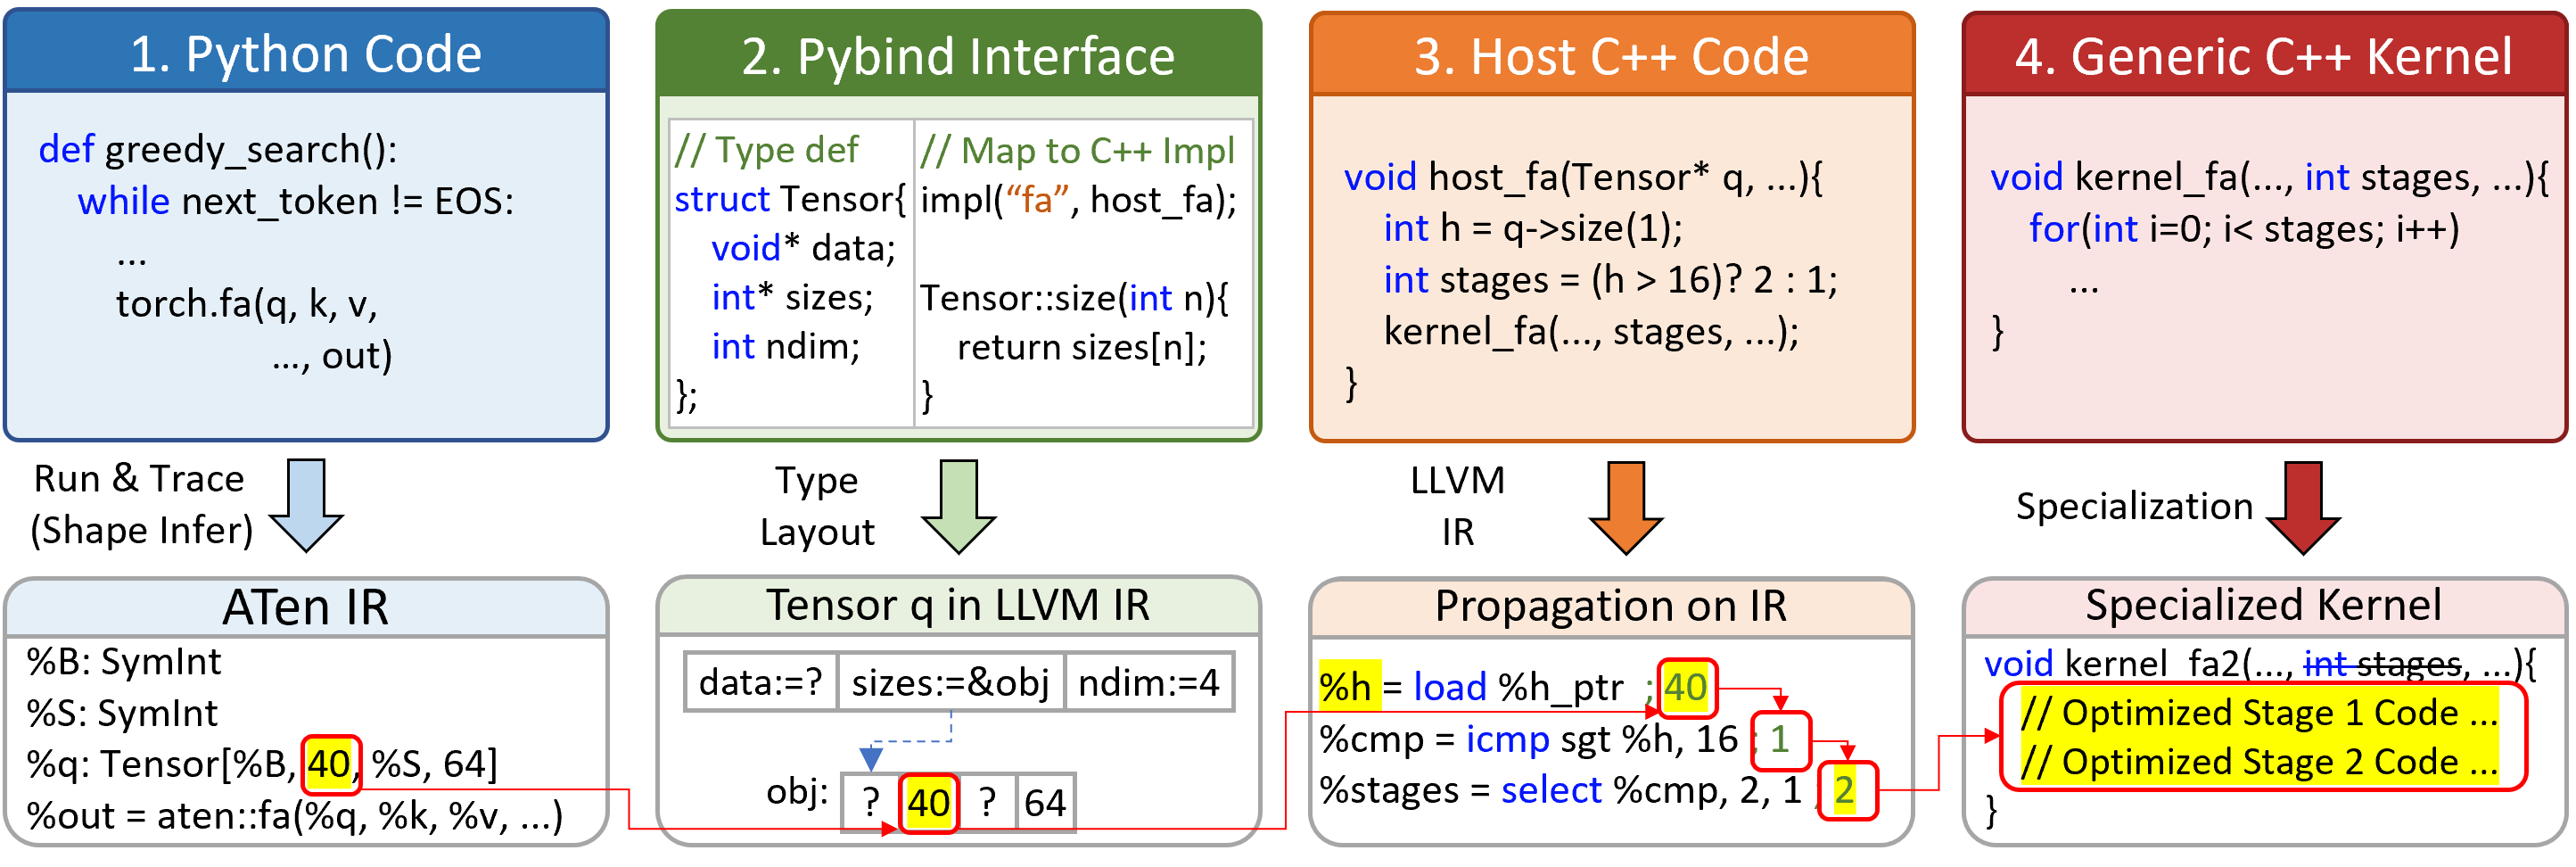
\includegraphics[width=\linewidth]{figures/motivation/motivating-example.png}
	\caption{A simplified Graph-to-C++ constant-propagation opportunity for Flash Attention. A model-fixed graph dimension (e.g., \texttt{q->size(1) = 40}) flows into C++ host code and determines the launch-site schedule parameter \texttt{stages = 2}, enabling specialization of \texttt{kernel\_fa} into \texttt{kernel\_fa2}.}
	\Description{Diagram showing a graph-level model constant materialized in the abstract C++ entry state and propagated through host code to a device-kernel launch site.}
	\label{fig:motivating-example}
\end{figure}

\subsubsection{\DIFdel{Disadvantages of Generic Kernels and Manually Specialized Libraries}\DIFadd{Limitations of the Two Expert-Written Operator-Library Designs}}
\label{sec:motivation:disadvantages}

\paragraph*{Bottleneck Analysis \DIFdel{for Generic Kernels}\DIFadd{of Schedule-Generic Implementations}.}

{\color{red}%
\DIFdel{%
Some operator libraries implement their kernels in the form of generic kernels, such as the built-in operator library of Ascend CANN. These kernels are not specialized mainly due to their complex schedule strategies and the great number of schedule parameters. In this design, almost all schedule parameters are passed as runtime arguments from the host. Since the compiler treats these parameters as variables, it cannot perform aggressive optimizations like constant folding. To understand the impact of this design, we examine the execution flow on Ascend, a DL accelerator based on SIMD execution model, as shown in }\autoref{fig:fa_on_ascend}\DIFdel{.
}
\par}
{\color{blue}%
Schedule-generic kernels support complex scheduling strategies by receiving numerous schedule parameters from the host at runtime. Because the compiler cannot treat these parameters as constants, optimizations such as constant folding and loop simplification remain limited. \autoref{fig:fa_on_ascend} illustrates the resulting overhead on Ascend.
\par}

{\color{red}%
\DIFdel{%
Ascend is a DL accelerator based on SIMD execution model, featuring diverse compute and storage units for handling different types of tensor computations and data movement operations. Specifically, the Cube and Vector units execute the primary tensor operations (e.g., MatMul on Cube and Softmax on Vector), while the architecture provides sophisticated programmable memory hierarchies. The kernel must explicitly manage the chunk size and data layout at every level, as well as the data movement and layout transformations between these levels. Besides, the Scalar unit acts as the central control unit, responsible for scalar data processing, instruction dispatch, and handling control flows (such data paths are indicated by red dashed lines; for simplicity, only some are shown). For example, the kernel moves a tile of the tensor $Q_{GM}$ from the global memory (GM) to the L1 memory unit at a time, denoted as $Q_{L1}$. During this data movement, the Scalar unit is responsible for calculating the starting memory address of tile $Q_{GM}$, implementing loop iterations, and loading or storing necessary scalar data (including schedule parameters and partial scalar intermediate results) from the global memory or the Unified Buffer (UB).
}
\par}
{\color{red}%
\DIFdel{%
In generic kernels, the Scalar unit may be over-occupied. Since the Scalar unit typically possesses much lower computing power than a general-purpose host CPU, excessive scalar calculations related to schedule parameters can overload the unit. Worse yet, excessive scalar intermediates may cause register spill, as there are only 32 general-purpose registers. As a result, the powerful Cube and Vector units will stall to await instruction dispatch or scalar operands. Furthermore, generic kernels often involve complex control flows (e.g., branching to handle different operator variants), which exerts heavy pressure on the instruction cache (I-Cache). Frequent instruction jumps in such complex logic inevitably lead to I-Cache misses and pipeline flushes. Finally, when loop bounds remain unknown at compile time, the compiler struggles to perform loop unrolling. Consequently, instruction scheduling is confined to the scope of a single iteration, preventing the effective overlapping of memory access and computation.
}
\par}
{\color{red}%
\DIFdel{%
We further study this impact by profiling key operators from the Qwen2.5-1.5B model on the Ascend NPU. }\autoref{fig:perf_stats}\DIFdel{ presents the Scalar unit occupancy (the proportion of active cycles during kernel execution) and I-Cache miss rates. The data reveals that the Scalar unit is active for 78\% to 91\% of total cycles, while I-Cache miss rates range from 3.1\% to 16.4\%.
}
\par}
{\color{blue}%
Ascend combines Cube and Vector compute units with a programmable memory hierarchy. Kernels explicitly manage tile sizes, data layouts, and data movement across memory levels, while the Scalar unit computes addresses and loop bounds, handles control flow, and dispatches instructions. For example, when moving a tile from $Q_{GM}$ in global memory (GM) to $Q_{L1}$ in L1 memory, the Scalar unit determines its starting address, advances the loop, and accesses schedule parameters and scalar intermediates in GM or the Unified Buffer (UB). The representative profiles in \autoref{fig:perf_stats} show high Scalar ratios and nonzero I-Cache miss rates for several of these kernels. These measurements motivate device-side specialization to reduce the scalar workload and improve instruction locality.
\par}

\begin{figure}[htbp]
	\centering
	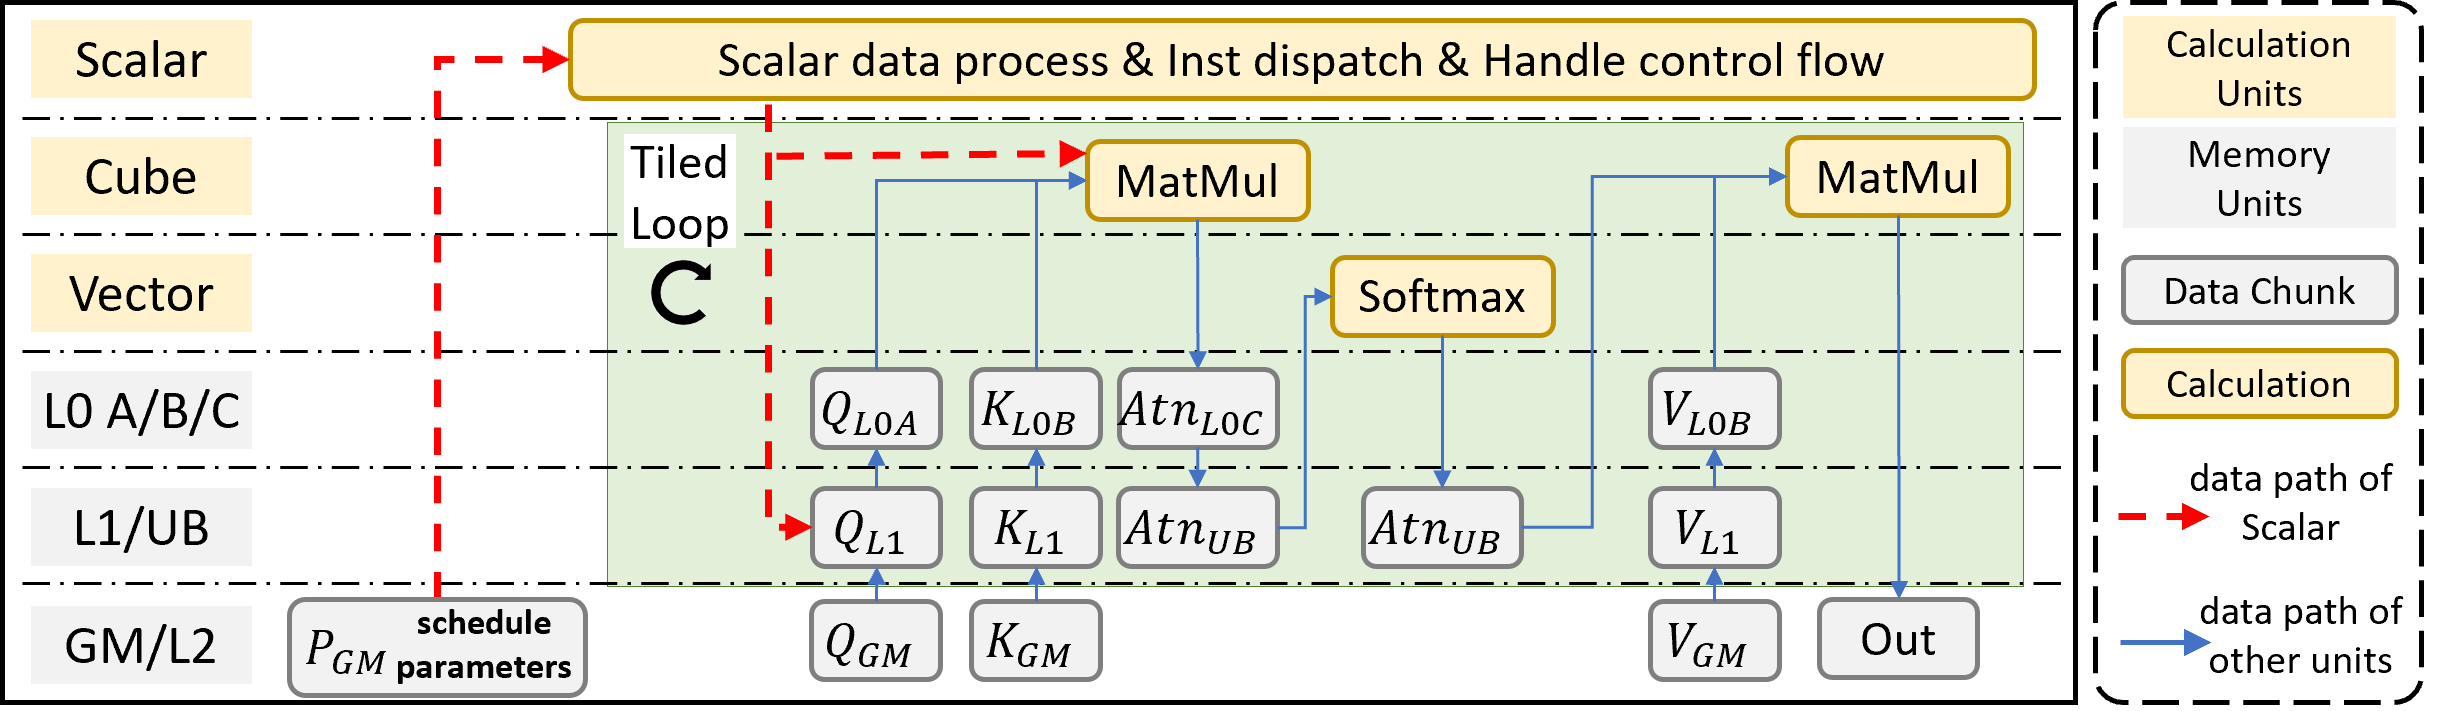
\includegraphics[width=0.8\textwidth]{figures/motivation/ascend-data-path.png}
	\caption{Execution flow of Flash Attention kernel \texttt{kernel\_fa} on the Ascend architecture.
		The \textbf{Scalar} unit acts as the central scheduler.
		It continuously performs scalar calculations and dispatches instructions based on runtime parameters.
		The heavy scalar workload required by generic kernels may lead to a scalar bottleneck.}
	\Description{Diagram showing the interaction between Scalar, Cube, Vector, L1, and GM units on Ascend.}
	\label{fig:fa_on_ascend}
\end{figure}

% Keep this paragraph in its original word-level LaTeXDiff form.
\paragraph*{Code Bloat in \DIFdel{Manually Specialized Libraries}\DIFadd{Schedule-Fixed Implementations}.}
High-performance GPU libraries \DIFdel{like }\DIFadd{such as }FlashInfer~\cite{ye2025flashinfer} rely on C++ template metaprogramming to enable aggressive compiler optimizations.
To avoid runtime JIT overhead, \DIFdel{these }\DIFadd{such }libraries pre-instantiate kernels for the Cartesian product of all template parameters.
As described in \autoref{eq:flash_attention}, FA's configuration space includes head dimensions ($d_k \in \{64, 128, 256\}$), mask types, GQA sizes, and position encodings.
Combined with \DIFdel{tile size}\DIFadd{tile-size} configurations, this results in over \DIFdel{1000}\DIFadd{1,000} binary instantiations, yet a specific model \DIFdel{like \textbf{Qwen2-1.5B} }\DIFdel{utilizes}\DIFadd{uses} only $\sim$10 kernels.
This pre-instantiation strategy, while manageable on GPUs, is ill-suited for Ascend due to its more complex schedule parameters, forcing \DIFdel{Ascend libraries }\DIFadd{their Ascend counterparts }to rely on \DIFdel{suboptimal generic kernels}\DIFadd{schedule-generic kernels with limited compile-time optimization}.

\begin{figure}[htbp]
	\centering
	\begin{minipage}{0.47\textwidth}
		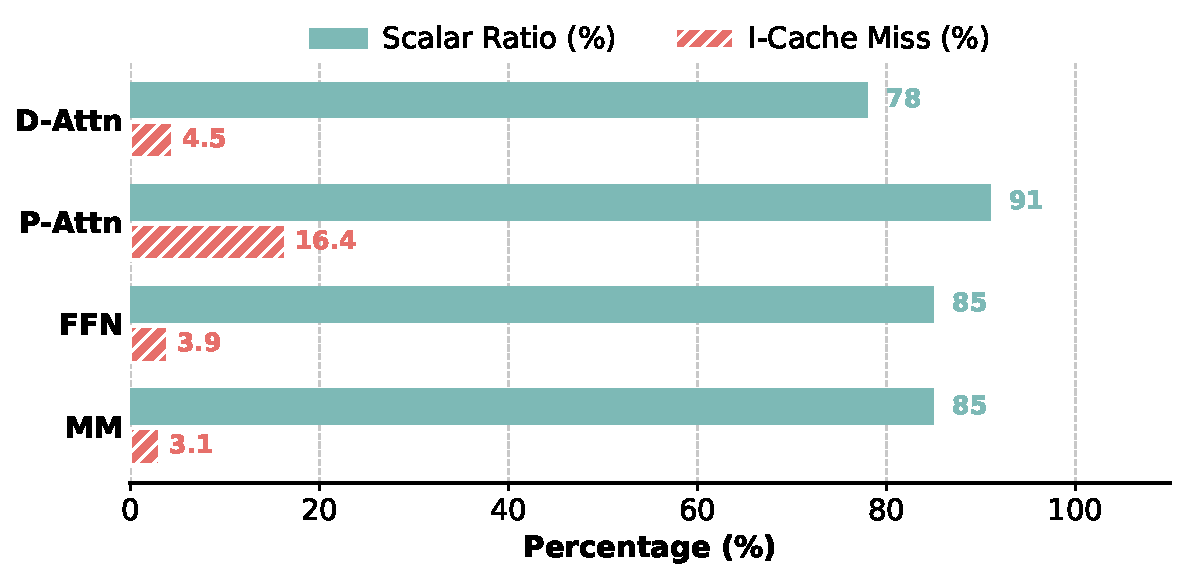
\includegraphics[width=\linewidth]{figures/motivation/metrics_analysis.pdf}
		\caption{Performance profiles of schedule-generic kernels, where lower values are better for both metrics: Decoding Attention (\textbf{D-Attn}), Prefill Attention (\textbf{P-Attn}), Feed Forward Networks (\textbf{FFN}), and MatMul (\textbf{MM}).}
		\Description{Bar chart showing scalar instruction ratio and I-Cache miss rate for different operators.}
		\label{fig:perf_stats}
	\end{minipage}
	\hfill
	\begin{minipage}{0.47\textwidth}
		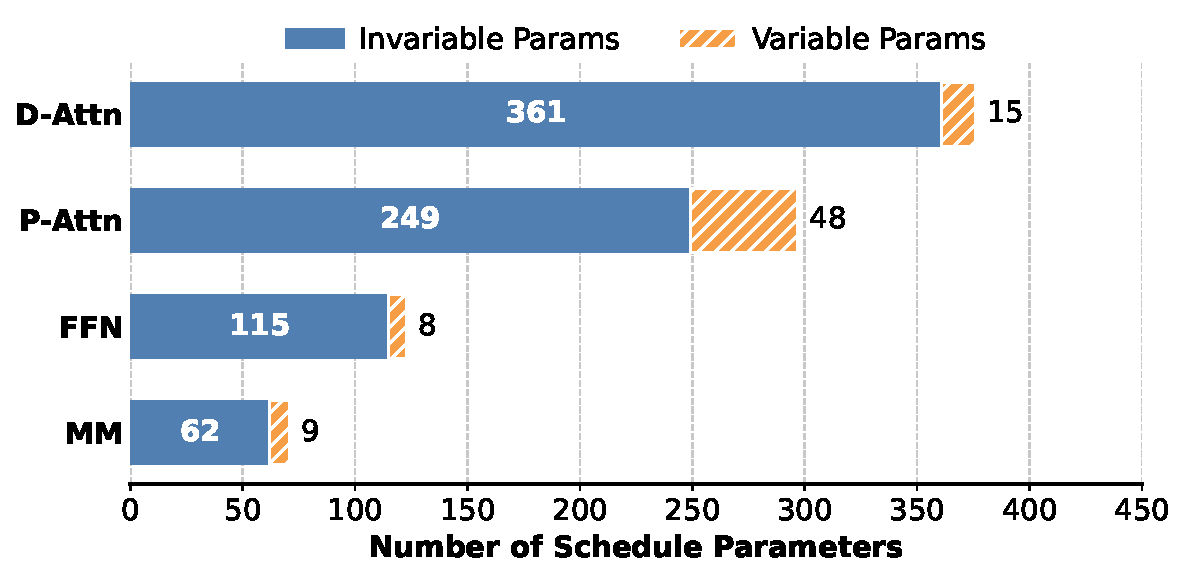
\includegraphics[width=\linewidth]{figures/motivation/parameter_breakdown.pdf}
		\caption{Number of schedule parameters of representative kernels. The vast majority are runtime invariants (Invariable Params), validating the potential for specialization.}
		\Description{Bar chart showing the breakdown of schedule parameters into variable and invariable categories.}
		\label{fig:param_stats}
	\end{minipage}
\end{figure}

% Keep this subsection in its original word-level LaTeXDiff form.
\subsubsection{Why Is Automatic \DIFdel{Kernel }\DIFadd{Model-Specific }Specialization Beneficial?}

We further analyze the schedule parameters of key operators from the \textbf{Qwen2.5-1.5B} model, classifying them into \textit{invariable parameters} (constants derived from model configuration) and \textit{variable parameters} (runtime-dependent values such as batch size and sequence length).
\autoref{fig:param_stats} reveals that the overwhelming majority of kernel parameters are invariable.
Propagating model-specific constants to resolve schedule parameters at compile time yields two benefits: (1) for \DIFdel{generic kernels}\DIFadd{schedule-generic implementations}, it enables model-specific \DIFadd{kernel }specialization with aggressive constant folding, reducing scalar overhead and I-Cache misses; (2) for \DIFdel{manually specialized libraries}\DIFadd{schedule-fixed implementations}, it makes kernel dispatch paths deterministic, enabling precise pruning of unused binaries.

\DIFadd{In addition, the sensitivity study in \S\ref{sec:eval:sensitivity} analyzes which schedule parameters have the greatest effect on performance. It shows that a small subset of parameters on the kernel's hot path accounts for most of the performance gain.}\par

\subsection{Challenges and Design Insights}
\label{sec:motivation:challenges}

{\color{red}%
\DIFdel{%
Achieving automatic kernel specialization requires analyzing the value flow from Python down to C++, which presents two major challenges that cannot be properly addressed by existing static analysis.
}
\par}
{\color{blue}%
Achieving automatic model-specific specialization requires transferring graph-level facts into C++ compilation and preserving them through host-side control flow. These steps present two challenges not directly addressed by existing static analyses.
\par}

\subsubsection{Challenge 1: \DIFdel{The cross-language semantic gap}\DIFadd{Reconstructing Cross-Language Calling Contexts}.}

{\color{red}%
\DIFdel{%
Achieving automatic kernel specialization requires reconstructing the calling context for C++ operator functions, i.e., determining the tensor shapes and operator attribute values. As shown in }\autoref{fig:motivating-example}\DIFdel{, these values are instantiated on the Python side and passed through the FFI layer to C++. However, reconstructing this cross-language value flow faces significant challenges.
}
\par}
{\color{blue}%
The first challenge is the Python/C++ semantic gap: Graph IR constants and symbolic dimensions must be mapped to the memory states of their underlying C++ objects before LLVM can use them as compile-time facts. This mapping is not a direct binding between the arguments of a Graph IR node and C++ parameters. Graph IR records typed values and shapes, whereas composite C++ parameters such as \texttt{Tensor}, \texttt{List}, and \texttt{Optional} use nested object layouts; after lowering, an access such as \texttt{query->size(1)} becomes pointer arithmetic and \texttt{load} instructions. The analyzer must therefore reconstruct the corresponding base objects, pointers, field offsets, and field values, preserving concrete dimensions as constants and symbolic dimensions as unknown.
\par}

{\color{red}%
\DIFdel{%
Existing cross-language analysis methods~}\mbox{\cite{kan2024taint4javac,Monat2021PythonC}}\hspace{0pt}\DIFdel{ typically employ abstract interpretation at the FFI API level, modeling each cross-language call as state transitions in an abstract domain. While general-purpose, this approach is ill-suited for DL systems for two reasons. First, the FFI layer contains substantial glue code for type conversions, dynamic dispatch, and reference counting, operations that are essential for language interoperability but irrelevant to the constant values we aim to extract. Analyzing this glue code is both computationally expensive and unnecessary for our goal. Second, the Python-side Graph Executor, which orchestrates operator invocations based on Graph IR, comprises complex logic spanning thousands of lines of code. Performing full abstract interpretation over this codebase is prohibitively expensive. These factors render traditional approaches impractical for reconstructing operator calling contexts in DL systems.
}
\par}
{\color{blue}%
Existing cross-language analyses broadly follow two approaches: multilanguage abstract interpretation jointly analyzes programs on both sides of an FFI boundary~\cite{Monat2021PythonC}, while specification-based methods summarize native behavior under a cross-language caller context~\cite{kan2024taint4javac}. The former would have to traverse the Python Graph Executor and FFI glue for dispatch, type conversion, object construction, and reference counting, which is expensive and largely irrelevant to graph-level constants. The latter assumes or derives a cross-language caller context but does not define how Graph IR metadata should materialize the field-sensitive C++ entry state required by LLVM.
\par}

{\color{red}%
\DIFdel{%
Insight: Semantic modeling of core data types in DL systems. Instead of analyzing FFI glue code and Python source code, we propose a cross-language semantic modeling approach grounded in two observations: (1) Finite and Stable Core Types: Data types used for cross-language interaction in DL systems are highly convergent and stable (Tensor, Array, etc.), enabling comprehensive and precise semantic modeling. (2) Extract Constant Information from Graph IR: DL systems compile models and represent them using Graph IR (e.g., ATen IR), which contains precise information regarding operator input parameters, enabling direct extraction of semantic values without analyzing Python source code. Specifically, model-specific constants are captured as exact values from tracing, while dynamic dimensions are represented as symbolic variables. Building on these insights, we directly map computation graph node information to the abstract states of C++ entry functions, achieving high-precision reconstruction of C++ contexts while avoiding the overhead of analyzing complex FFI glue code.
}
\par}
{\color{blue}%
\textit{Insight: Type-directed calling-context construction.} DL operator interfaces use a limited set of parameter types, and their C++ interface layouts are stable within a backend. We can therefore define a context-update rule for each type and use Graph IR shapes and attributes to construct an accurate C++ operator calling context directly. This approach avoids analyzing FFI glue code; \autoref{tab:semantic-rules} formalizes the context-update rules used by TilingInfer.
\par}

\begin{figure}[htbp]
	\centering
	\begin{minipage}{0.39\textwidth}
		\begin{lstlisting}[
    language=C++,
    frame=single,
    caption={Early-exit path example.},
    basicstyle=\ttfamily\footnotesize,
    columns=fullflexible,
    framesep=1.5pt,
    aboveskip=0pt,
    belowskip=0pt,
    label={lst:early_return_code}
  ]
const status SUCCESS=0, ERROR=-1;
status check(int s1, int s2) {
  if(s1 != s2) return ERROR;
  return SUCCESS;
}
status set_t(int sk, int sv, int* t) {
  int e = check(sk, sv);
  if(e != SUCCESS) {
    print("error"); return e;
  }
  *t=32; // Tiling
  return SUCCESS;
}
  \end{lstlisting}
	\end{minipage}
	\hspace{0.04\textwidth}
	\begin{minipage}{0.47\textwidth}
		\centering
		\begin{tikzpicture}[
					bb/.style={
							rectangle,
							rounded corners=2.5pt,
							draw=black,
							thick,
							minimum width=2.5cm,
							inner sep=3pt,
							font=\ttfamily\footnotesize,
							align=left
						},
					edge_label/.style={
							font=\ttfamily\footnotesize,
							midway
						},
					>=stealth
				]
				\node[bb] (BB0) at (0, 0) {
				\textbf{BB0:}\\
				{\color{green!50!black}\%0} = call @check({\color{green!50!black}\%sk}, {\color{green!50!black}\%sv})\\
				{\color{green!50!black}\%1} = icmp ne {\color{green!50!black}\%0}, 0
				};

				\node[bb] (BB1) at (-1.55, -1.2) {
					\textbf{BB1:}\\
					call @print(...)
				};

				\node[bb] (BB2) at (1.55, -1.2) {
					\textbf{BB2:}\\
					store 32, {\color{green!50!black}\%t}
				};

				\node[bb] (BB3) at (0, -2.65) {
					\textbf{BB3:}\\
					{\color{green!50!black}\%2} = phi [{\color{green!50!black}\%0}, {\color{green!50!black}\%BB1}], [0, {\color{green!50!black}\%BB2}]\\
					ret {\color{green!50!black}\%2}
				};

				\draw[->, thick] (BB0.south) -- (BB1.north)
				node[edge_label, left, pos=0.6] {{\color{green!50!black}$\%1$} (true)};
				\draw[->, thick] (BB0.south) -- (BB2.north)
				node[edge_label, right, pos=0.6] {$\neg${\color{green!50!black}$\%1$} (false)};
				\draw[->, thick] (BB1.south) -- (BB3.north);
				\draw[->, thick] (BB2.south) -- (BB3.north);

				\node[font=\ttfamily\footnotesize, align=center] at (-1.6, -1.9) {
				$*({\color{green!50!black}\%t}) = 0$\\
				{Early-Exit Path}
				};
				\node[font=\ttfamily\footnotesize, align=center] at (1.6, -1.9) {
				$*({\color{green!50!black}\%t}) = 32$\\
				{Normal Path}
				};
		\end{tikzpicture}
		\caption{Control Flow Graph (CFG) of \texttt{set\_t}'s LLVM IR. Each node is a basic block containing LLVM IR instructions. Edges are labeled with branch conditions.}
		\label{fig:set_t_cfg}
	\end{minipage}
	\Description{Control flow graph showing an early-exit path in LLVM IR.}
\end{figure}

\color{black}
\subsubsection{Challenge 2: Shape Checkers Leading to Early-Exit Paths}
\leavevmode

{\color{red}%
\DIFdel{%
Operator libraries enforce shape constraints through runtime shape checkers to ensure memory safety and computational correctness. As defined in }\autoref{eq:flash_attention}\DIFdel{, the Flash Attention operator imposes one constraint that the sequence lengths of $K$ and $V$ must be equal ($S_k = S_v$). Violations of these constraints trigger early exits with error codes.
}
\par}
{\color{blue}%
The second challenge is preserving constant-propagation precision across shape-checker-induced early-exit paths without expensive path-sensitive analysis. Operator libraries enforce constraints for memory safety and correctness; for example, Flash Attention requires equal key and value sequence lengths ($S_k=S_v$). Because these dimensions may remain symbolic, the compiler cannot decide whether a check succeeds. An early-exit path then bypasses assignments performed on the normal path, and merging the two states can obscure constants.
\par}

{\color{red}%
\DIFdel{%
}\autoref{lst:early_return_code}\DIFdel{ illustrates this pattern with a simplified example. The function check verifies whether two sequence lengths (denoted as s1 and s2) match, returning SUCCESS (0) if they are equal or ERROR (-1) otherwise. The function set\_t uses this checker to validate the sequence lengths before computing the tiling parameter t=32. Since these dimensions are dynamic at compile time, the compiler cannot determine whether the check will succeed or fail.
}
\par}
{\color{red}%
\DIFdel{%
}\autoref{fig:set_t_cfg}\DIFdel{ shows the corresponding CFG. The entry block BB0 calls @check and branches based on the result: the true branch leads to BB1 (error path), while the false branch leads to BB2 (normal path) where t=32 is defined. Both paths converge at BB3. At this merging site, standard path-insensitive analysis cannot determine whether the definition of t originates from BB2 or is undefined from BB1, resulting in a polluted abstract state $\{t \in \{0, 32\}\}$ that prevents constant propagation.
}
\par}
{\color{blue}%
In \autoref{lst:early_return_code}, \texttt{check} returns \texttt{SUCCESS} or \texttt{ERROR}, and \texttt{set\_t} computes \texttt{t=32} only after the check succeeds. The CFG in \autoref{fig:set_t_cfg} branches at \textbf{BB0}: \textbf{BB1} returns through the early-exit path without defining \texttt{t}, whereas \textbf{BB2} defines it before both paths reach \textbf{BB3}. If \texttt{t} initially holds 0, path-insensitive merging yields $\{0,32\}$ rather than the normal-path constant 32. Enumerating all paths would avoid this pollution, but nested shape checkers make full path-sensitive analysis impractical.
\par}

{\color{red}%
\DIFdel{%
Insight: Conditional Return-Value Flow. The key to identifying early-exit paths lies in analyzing the relationship between path guards and the semantic meaning of return values. Since shape checkers assign different constant values to the return variable on different execution paths (e.g., SUCCESS on the normal path and ERROR on the error path), we can determine whether a path is an early-exit by examining whether the path guard implies an error return value. Specifically, we maintain path-sensitive guards and propagate them through the control flow. If a path guard implies that the return value equals an error code, the path is identified as an early-exit path; otherwise, it is conservatively treated as a normal path. During constant propagation, value states from confirmed early-exit paths are prevented from propagating to merge points, thereby avoiding state pollution. In }\autoref{fig:set_t_cfg}\DIFdel{, the branch condition at BB0 is $\%1 = (\%0 \neq 0)$, where $\%0$ is the return value of @check. When the guard $\%1 = true$ holds, we have $\%0 \neq 0$, which implies $\%0 \neq SUCCESS$; hence the return value represents an error, and the path $BB0 \rightarrow BB1 \rightarrow BB3$ guarded by $\%1$ is an early-exit path. Conversely, when the guard $\neg\%1$ holds, we have $\%0 = 0 = SUCCESS$; hence the return value represents success, and the path $BB0 \rightarrow BB2 \rightarrow BB3$ guarded by $\neg\%1$ is a normal path.
}
\par}
{\color{blue}%
\textit{Insight: Conditional Return-Value Flow.} CRVFG-based normal-path reasoning traces only the conditional flow of status return values and compares them with configured success and error sets. In the example, the guard $\%1=(\%0\neq0)$ being true implies that \texttt{check}'s return value is not \texttt{SUCCESS}, so \textbf{BB0}$\rightarrow$\textbf{BB1} is an early-exit edge; its false branch is the normal edge. Confirmed early-exit-edge states are excluded from normal-path merges, while unclassified edges are retained conservatively.
\par}

\begin{comment}
\section{Background and Motivation}
\label{sec:motivation}

\DIFdelbegin \DIFdel{In this section, we use a simplified Flash Attention (FA) operator as an example. Given query, key, and value tensors $Q \in \mathbb{R}^{B \times h_q \times S_q \times d_k}$, $K, V \in \mathbb{R}^{B \times h_{kv} \times S_{kv} \times d_k}$, }\DIFdelend \DIFaddbegin \subsection{\DIFadd{Graph IR and External Operator Libraries}}
\label{sec:background:graph-ir}

\DIFadd{A Graph Intermediate Representation (Graph IR) is a typed, directed dataflow graph: nodes encode inputs, attributes, operator calls, and outputs; edges carry tensors or scalars; and metadata records types and shapes. Framework IRs, such as PyTorch FX and TensorFlow graphs, preserve calls and arguments, while AI compiler IRs, such as TVM Relay/Relax, XLA HLO/StableHLO, and Inductor IR, normalize operations for optimization and lowering~\mbox{%DIFAUXCMD
\cite{roesch2018relay,Lai2023RelaxCA,tensorflow2021xla,stablehlo2024,ansel2024dynamo}}\hspace{0pt}%DIFAUXCMD
. We focus on framework IR operator nodes because they define calls to external expert-written operator libraries.
}

\DIFadd{With }\texttt{\DIFadd{torch.compile}}\DIFadd{, Dynamo extracts PyTorch operations from Python bytecode into an FX Graph~\mbox{%DIFAUXCMD
\cite{paszke2019pytorch,ansel2024dynamo}}\hspace{0pt}%DIFAUXCMD
. An FX operator node has $N=(\texttt{op},\texttt{target},\texttt{args},\texttt{kwargs},\texttt{meta})$: }\texttt{\DIFadd{op}}\DIFadd{/}\texttt{\DIFadd{target}} \DIFadd{identify the call, }\texttt{\DIFadd{args}}\DIFadd{/}\texttt{\DIFadd{kwargs}} \DIFadd{hold actual arguments, }\DIFaddend and \DIFdelbegin \DIFdel{an optional mask $M$, the attention operation is defined as:
}\DIFdelend \DIFaddbegin \texttt{\DIFadd{meta}} \DIFadd{stores type and shape information. We use the following simplified Flash-Attention computation:
}\DIFaddend \begin{equation}
	\DIFdelbegin \DIFdel{\text{Attention}}\DIFdelend \DIFaddbegin \operatorname{FA}\DIFaddend (Q,K,V,M)
	=
	\DIFdelbegin \DIFdel{\text{softmax}}\DIFdelend \DIFaddbegin \operatorname{softmax}\DIFaddend \left(\frac{QK^\top}{\sqrt{d_k}}+M\right)V\DIFaddbegin \DIFadd{,
	}\DIFaddend \label{eq:flash_attention}
\end{equation}
where \DIFaddbegin \DIFadd{$Q\in\mathbb{R}^{B\times h_q\times S_q\times d_k}$, $K,V\in\mathbb{R}^{B\times h_{kv}\times S_{kv}\times d_k}$, and $M$ is an optional mask~\mbox{%DIFAUXCMD
\cite{dao2024flashattention2}}\hspace{0pt}%DIFAUXCMD
. In }\autoref{eq:flash_attention}\DIFadd{, }\DIFaddend $B$\DIFdelbegin \DIFdel{is the batch size, $h_q$ is the number of query heads, $h_{kv}$ is the number of key-value heads}\DIFdelend , $S_q$\DIFaddbegin \DIFadd{, }\DIFaddend and $S_{kv}$ \DIFdelbegin \DIFdel{are sequence lengths, and }\DIFdelend \DIFaddbegin \DIFadd{may vary at runtime, whereas $h_q$, $h_{kv}$, }\DIFaddend $d_k$\DIFdelbegin \DIFdel{is the head dimension. The operator imposes strict shape constraints: for example, batch sizes must match across $Q$, $K$, and $V$, the number of query heads must be divisible by the number of key-value heads ($h_q \mod h_{kv} = 0$), and sequence lengths of $K$ and $V$ must be equal. Typical configurations include $h_q \in \{8, 16, 32, 40, \ldots\}$, $d_k \in \{64, 128, 256\}$, various mask types (none, causal, sliding window), attention variants (MHA, GQA, MLA), and position encodings (RoPE, ALiBi).
These parameters are fixed per model but vary across models, making them ideal for compile-time specialization.
}\DIFdelend \DIFaddbegin \DIFadd{, and attention attributes are model-fixed. A corresponding FX node has }\texttt{\DIFadd{op}} \DIFadd{= }\texttt{\DIFadd{call\_function}}\DIFadd{, }\texttt{\DIFadd{target}} \DIFadd{= }\texttt{\DIFadd{aten.scaled\_dot\_product\_attention}}\DIFadd{, }\texttt{\DIFadd{args}} \DIFadd{= }\texttt{\DIFadd{(q,k,v)}}\DIFadd{, and }\texttt{\DIFadd{kwargs}} \DIFadd{= \{}\texttt{\DIFadd{attn\_mask=None}}\DIFadd{, }\texttt{\DIFadd{dropout\_p=0.0}}\DIFadd{, }\texttt{\DIFadd{is\_causal=True}}\DIFadd{\}. For the concrete model instance used in our running example, the input FakeTensors }\texttt{\DIFadd{q}}\DIFadd{, }\texttt{\DIFadd{k}}\DIFadd{, and }\texttt{\DIFadd{v}} \DIFadd{have shapes $(s_B,40,s_q,128)$, $(s_B,8,s_{kv},128)$, and $(s_B,8,s_{kv},128)$, respectively, while the output FakeTensor in }\texttt{\DIFadd{meta}[\DIFadd{"val"}]} \DIFadd{has shape $(s_B,40,s_q,128)$. Here, $s_B$, $s_q$, and $s_{kv}$ are }\texttt{\DIFadd{SymInt}} \DIFadd{symbols tracked by }\texttt{\DIFadd{ShapeEnv}}\DIFadd{, whereas 40, 8, and 128 are concrete integers.
}\DIFaddend 

\DIFdelbegin %DIFDELCMD < \begin{figure}[ht]
%DIFDELCMD <     \centering
%DIFDELCMD <     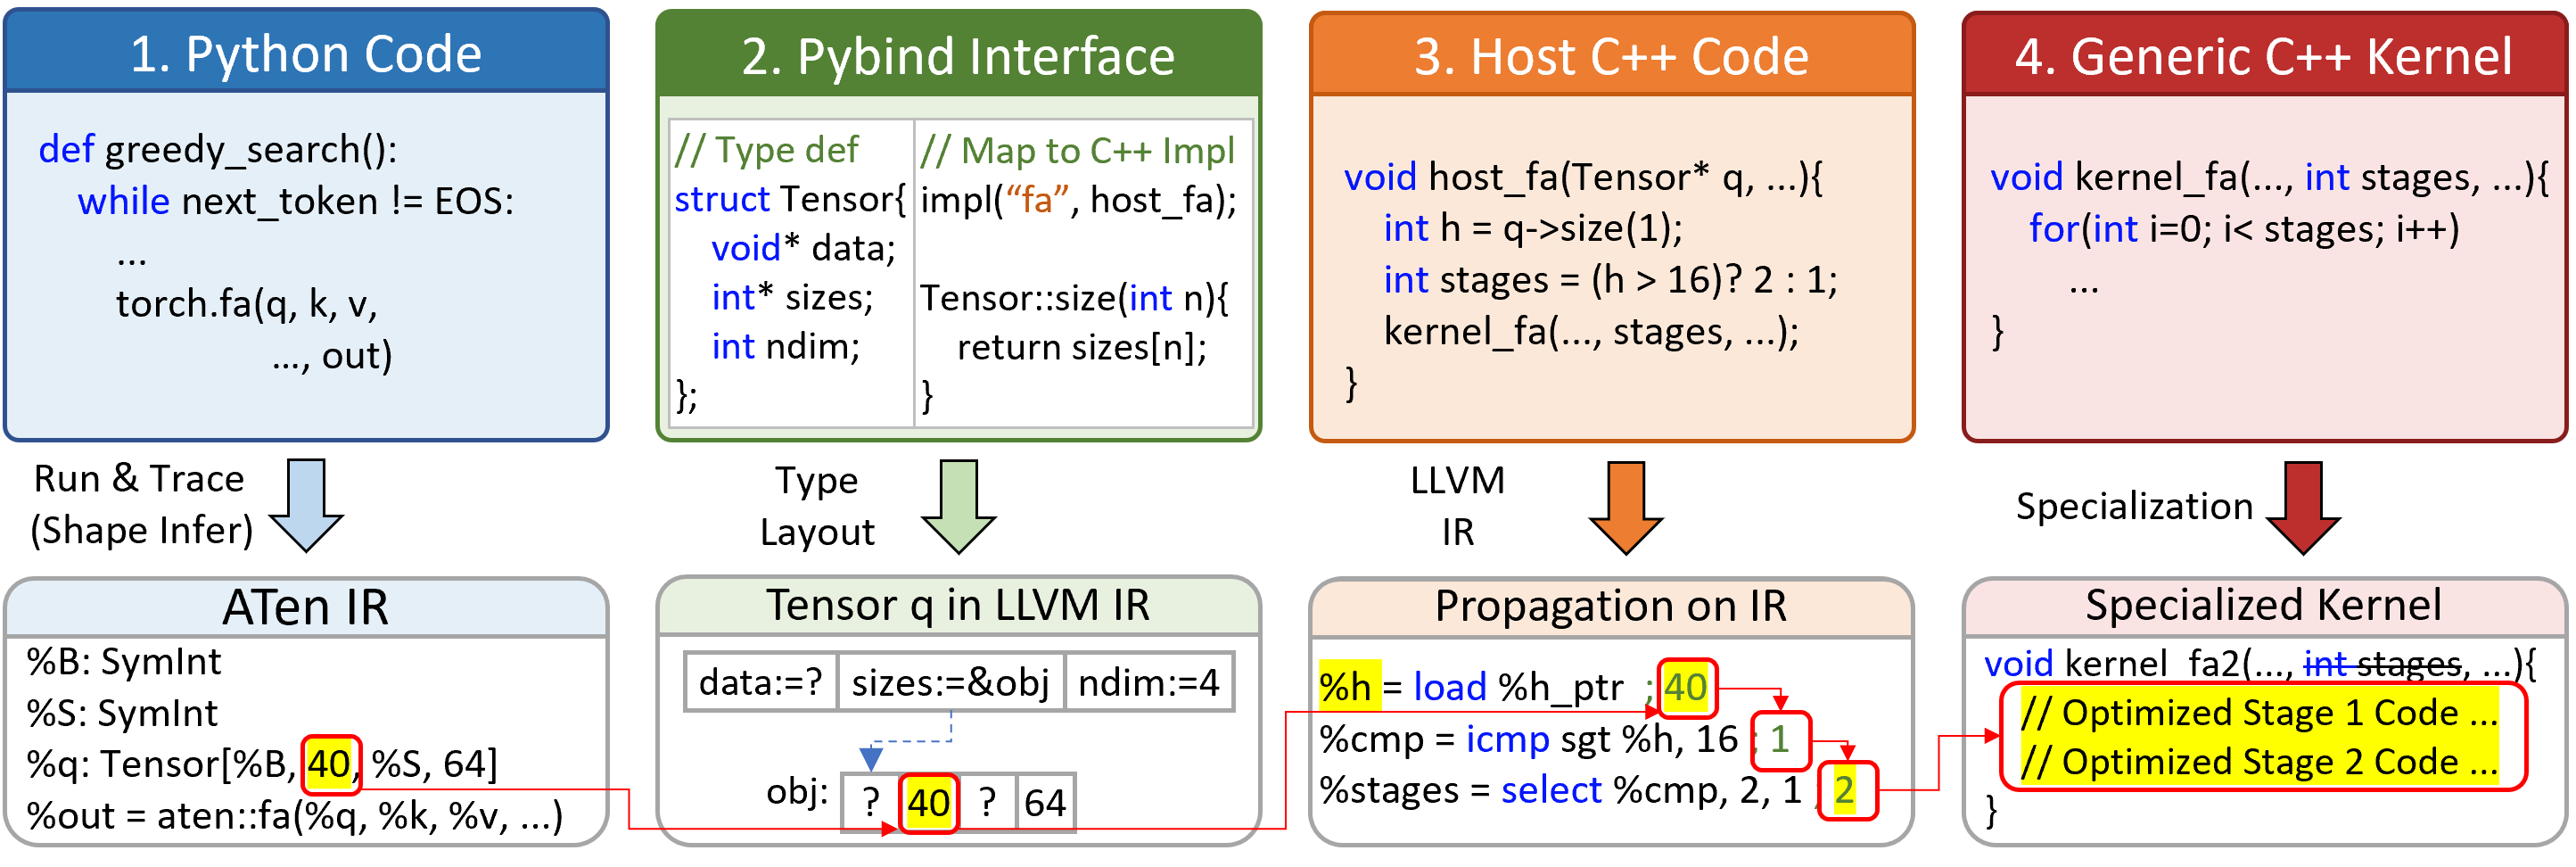
\includegraphics[width=\linewidth]{figures/motivation/motivating-example.png}
%DIFDELCMD <     \caption{A simplified example illustrating how constant information propagation of the Flash-Attention operator across Python and C++. The final constants (e.g., \texttt{stages}) derived from model-specific constants (e.g., \texttt{q->size(1) = 40}) can be used to specialize the device kernel \texttt{kernel\_fa}.}
%DIFDELCMD <     \Description{Diagram showing constant propagation from Python through FFI to C++ and device kernel.}
%DIFDELCMD <     \label{fig:motivating-example}
%DIFDELCMD <     \vspace{-10pt}
%DIFDELCMD < \end{figure}
%DIFDELCMD < %%%
\DIFdelend \DIFaddbegin \begin{example}[Scaled Dot-Product Attention Operator Signature]
\label{ex:sdpa-signature}
\DIFadd{The simplified C++ operator signature is:
}\par
\noindent\DIFadd{\fbox{%
\parbox{\dimexpr\linewidth-2\fboxsep-2\fboxrule\relax}{%
\raggedright\ttfamily
scaled\_dot\_product\_attention(query: Tensor, key: Tensor, value: Tensor, attn\_mask:\\
\hspace*{2em}Optional[Tensor], dropout\_p: float, is\_causal: bool) -> Tensor\par}}
}\par
\end{example}
\DIFadd{It binds }\texttt{\DIFadd{q}}\DIFadd{, }\texttt{\DIFadd{k}}\DIFadd{, and }\texttt{\DIFadd{v}} \DIFadd{to }\texttt{\DIFadd{query}}\DIFadd{, }\texttt{\DIFadd{key}}\DIFadd{, and }\texttt{\DIFadd{value}}\DIFadd{, and the keyword values to }\texttt{\DIFadd{attn\_mask}}\DIFadd{, }\texttt{\DIFadd{dropout\_p}}\DIFadd{, and }\texttt{\DIFadd{is\_causal}}\DIFadd{; other optional parameters are omitted. Inside the C++ host implementation, every dimension is read uniformly through calls such as }\texttt{\DIFadd{q->size(i)}}\DIFadd{. Such loads do not preserve whether the FX dimension was a concrete integer or a }\texttt{\DIFadd{SymInt}}\DIFadd{; the operator-library compiler therefore treats every loaded size as a runtime variable. This loss of graph-level shape information motivates its propagation into the C++ compilation flow.
}\DIFaddend 

\subsection{Motivation of Automatic \DIFdelbegin \DIFdel{Kernel }\DIFdelend \DIFaddbegin \DIFadd{Model-Specific }\DIFaddend Specialization}
\label{sec:motivation:auto-spec}

\DIFdelbegin \DIFdel{This section elucidates }\DIFdelend \DIFaddbegin \DIFadd{In existing expert-written operator-library compilation pipelines, treating constant dimensions and operator attributes as variables creates two forms of waste: scalar and control overhead in schedule-generic kernels and unreachable template instances in schedule-fixed binaries. This subsection examines }\DIFaddend the opportunity for \DIFdelbegin \DIFdel{kernel specialization by tracing the flow of constant values across the software stack. It further demonstrates the necessity of this approach by analyzing the bottlenecks inherent in generic kernels on Ascend~\mbox{%DIFAUXCMD
\cite{liao2019davinci}}\hspace{0pt}%DIFAUXCMD
, a widely employed AI accelerator}\DIFdelend \DIFaddbegin \DIFadd{Graph-to-C++ constant propagation, the limitations of current compilation pipelines, and the key observation that most scheduling parameters are runtime invariants}\DIFaddend .

\subsubsection{\DIFdelbegin \DIFdel{Cross-Layer }\DIFdelend \DIFaddbegin \DIFadd{Graph-to-C++ }\DIFaddend Constant \DIFdelbegin \DIFdel{Value Flow}\DIFdelend \DIFaddbegin \DIFadd{Propagation}\DIFaddend }
\label{sec:motivation:flow}

\DIFdelbegin \DIFdel{The }\textbf{\textit{\DIFdel{partial dynamics}}%DIFAUXCMD
} %DIFAUXCMD
\DIFdel{characteristic of DL models implies that while input tensors vary , there are many }%DIFDELCMD < model-specific constants%%%
\DIFdel{.
}%DIFDELCMD < \autoref{fig:motivating-example} %%%
\DIFdel{illustrates how these constants propagate through the software stack}\DIFdelend \DIFaddbegin \DIFadd{DL models are partially dynamic: batch size and sequence lengths may vary at runtime, while dimensions and attributes such as head count are fixed by the model configuration}\DIFaddend . When a \DIFdelbegin \DIFdel{Python-level operator (e.g., }\texttt{\DIFdel{torch.fa}}%DIFAUXCMD
\DIFdel{) }\DIFdelend \DIFaddbegin \DIFadd{Python operator }\DIFaddend is invoked, \DIFdelbegin \DIFdel{arguments flow through the FFI layer to the host C++ library.
While some parameters are runtime-dependent (e.g., batch size }\texttt{\DIFdel{\%B}} %DIFAUXCMD
\DIFdel{and sequence length of query }\texttt{\DIFdel{\%S}}%DIFAUXCMD
\DIFdel{), others are derived from the fixed model configuration (e.g., number of query heads $h=40$). As shown in the figure, within the host }\DIFdelend \DIFaddbegin \DIFadd{its tensors and attributes cross the FFI boundary into the }\DIFaddend C++ \DIFdelbegin \DIFdel{runtime, the software pipeline depth }\texttt{\DIFdel{stages}} %DIFAUXCMD
\DIFdel{is computed as }\DIFdelend \DIFaddbegin \DIFadd{host library, but their model-fixed status is not available to the separately compiled library. }\autoref{fig:motivating-example} \DIFadd{illustrates a fixed head count }\texttt{\DIFadd{h=40}} \DIFadd{flowing into the host expression }\DIFaddend \texttt{stages = (h > 32) ? 2 : 1}. \DIFdelbegin \DIFdel{Crucially, since }\DIFdelend \DIFaddbegin \DIFadd{Propagating }\DIFaddend \texttt{\DIFdelbegin \DIFdel{stages}\DIFdelend \DIFaddbegin \DIFadd{h=40}\DIFaddend } \DIFdelbegin \DIFdel{depends }\textit{\DIFdel{solely}} %DIFAUXCMD
\DIFdel{on $h$, a constant derived from the model configuration, its value can be statically determined at compile time through constant propagation .
By propagating $h=40$ from the Python front-end to the host C++ compiler, the expression }\texttt{\DIFdel{(h > 32) ? 2 : 1}} %DIFAUXCMD
\DIFdel{can be evaluated to yield }\texttt{\DIFdel{stages = 2}}%DIFAUXCMD
\DIFdel{, enabling the compiler to specialize the generic kernel }\texttt{\DIFdel{kernel\_fa}} %DIFAUXCMD
\DIFdel{into a concrete variant }\texttt{\DIFdel{kernel\_fa2}}%DIFAUXCMD
\DIFdel{, where the suffix denotes the specialized }\DIFdelend \DIFaddbegin \DIFadd{across the language boundary allows host-side constant propagation to infer the invariant schedule parameter }\DIFaddend \texttt{stages}\DIFdelbegin %DIFDELCMD < \MBLOCKRIGHTBRACE %%%
\DIFdel{value. }%DIFDELCMD < 

%DIFDELCMD < %%%
\DIFdel{This observation suggests an opportunity : by statically tracking }%DIFDELCMD < model-specific constants %%%
\DIFdel{from the Python front-end down to the kernel launch, we can identify runtime invariants that are currently treated as variables.
For generic kernels , this enables aggressive specialization of the device code.
Furthermore, for manually specialized libraries, this allows us to identify the specific kernel instantiations not matching the derived compile-time constants.
This facilitates the pruning of unreachable code paths for a specific model, mitigating binary bloat}\DIFdelend \DIFaddbegin \texttt{\DIFadd{=2}}\DIFadd{. Making such schedule invariants available at compile time creates an opportunity to specialize schedule-generic kernels and discard incompatible pre-instantiated variants}\DIFaddend .

\DIFaddbegin \begin{figure}[ht]
	\centering
	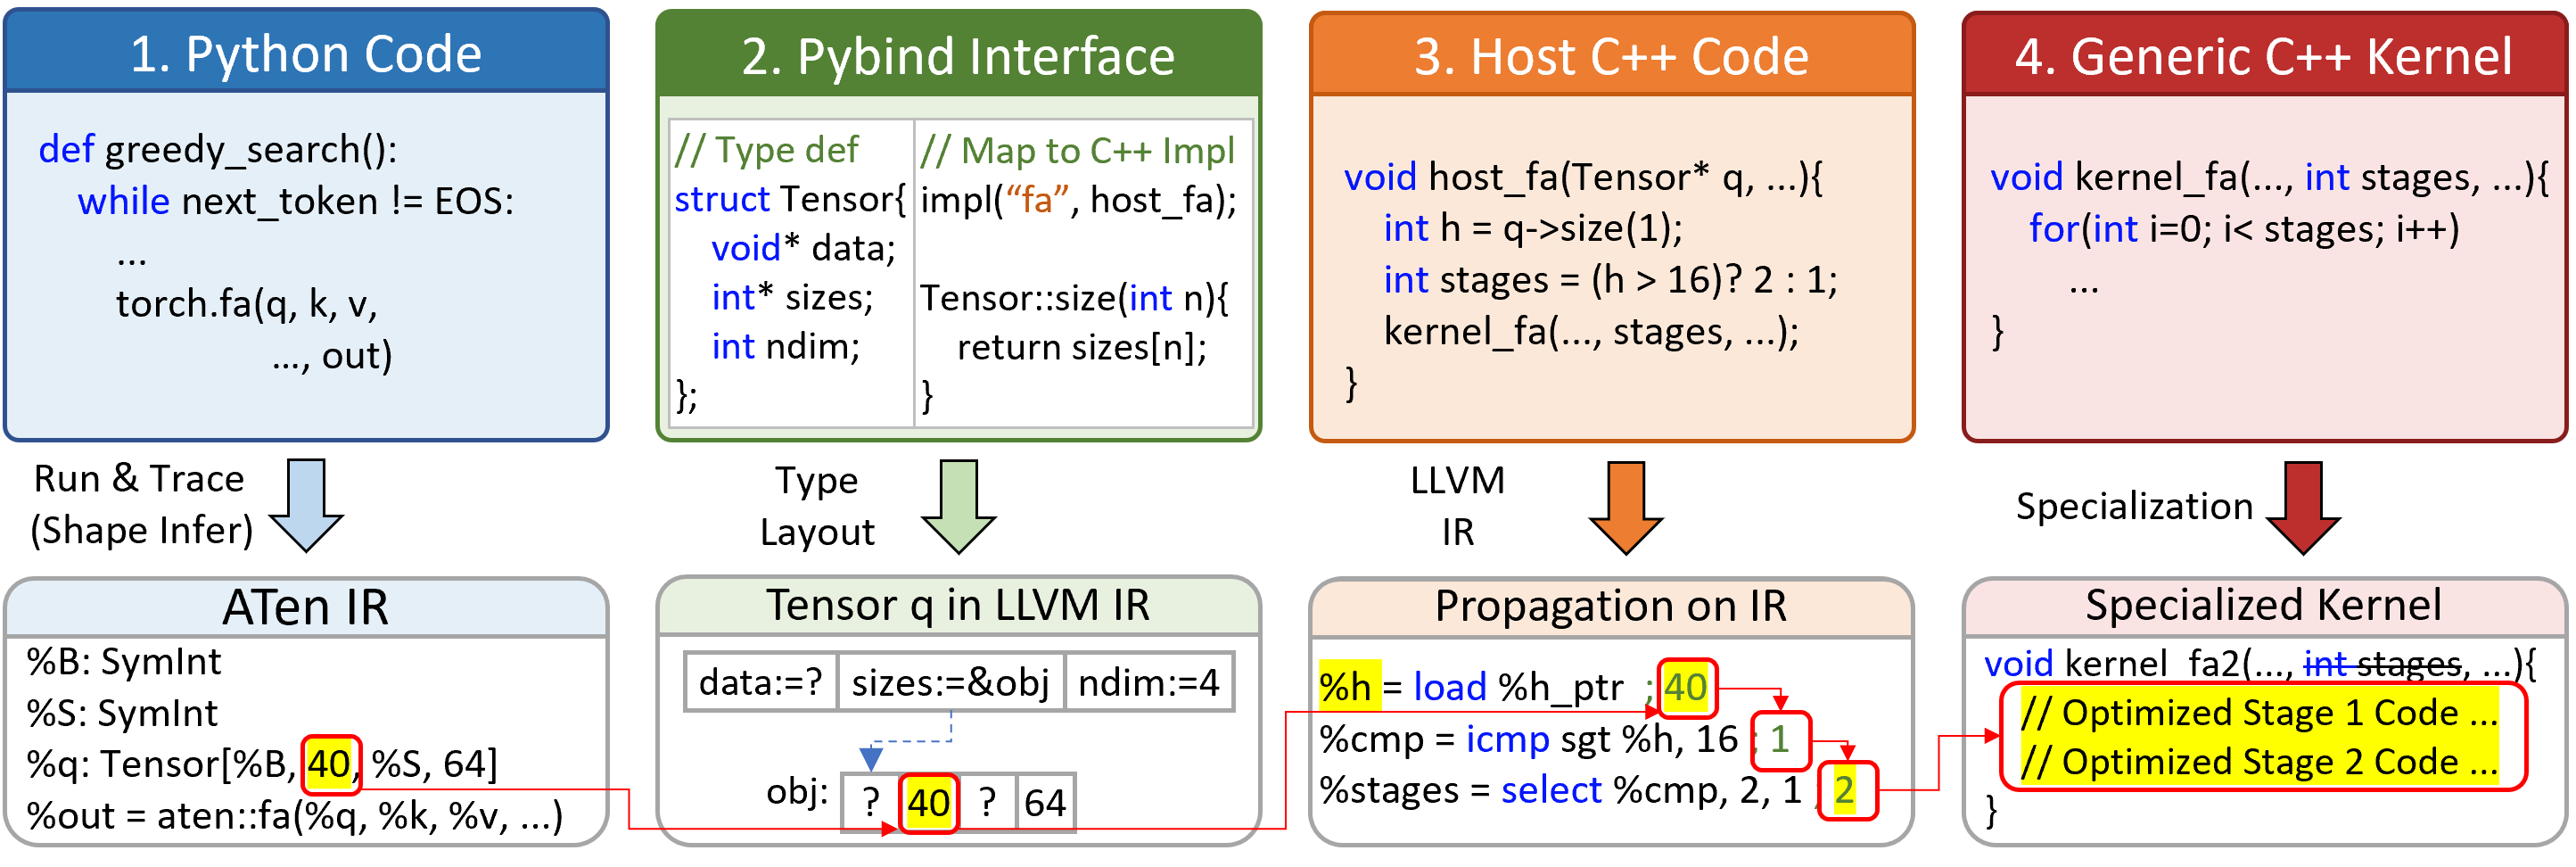
\includegraphics[width=\linewidth]{figures/motivation/motivating-example.png}
		\caption{A simplified Graph-to-C++ constant-propagation opportunity for Flash Attention. A model-fixed graph dimension (e.g., \texttt{q->size(1) = 40}) flows into C++ host code, determines the launch-site schedule parameter \texttt{stages = 2}, which can be used to specialize \texttt{kernel\_fa} and generate an optimized kernel \texttt{kernel\_fa2}.}
		\Description{Diagram showing a graph-level model constant materialized in the abstract C++ entry state and propagated through host code to a device-kernel launch site.}
		\label{fig:motivating-example}
\end{figure}

\DIFaddend \subsubsection{\DIFdelbegin \DIFdel{Disadvantages }\DIFdelend \DIFaddbegin \DIFadd{Limitations }\DIFaddend of \DIFdelbegin \DIFdel{Generic Kernels and Manually Specialized Libraries}\DIFdelend \DIFaddbegin \DIFadd{the Two Expert-Written Operator-Library Designs}\DIFaddend }
\label{sec:motivation:disadvantages}

\paragraph*{Bottleneck Analysis \DIFdelbegin \DIFdel{for Generic Kernels}\DIFdelend \DIFaddbegin \DIFadd{of Schedule-Generic Implementations}\DIFaddend .}
\DIFdelbegin \DIFdel{Some operator libraries implement their kernels in the form of generic kernels, such as the built-in operator library of Ascend CANN.
These kernels are not specialized mainly due to their complex schedule strategies and the great number of schedule parameters.
In this design, almost all schedule parameters are passed as runtime arguments }\DIFdelend \DIFaddbegin 

\DIFadd{Their kernels support complex scheduling strategies by receiving numerous schedule parameters }\DIFaddend from the host \DIFdelbegin \DIFdel{.
Since the compiler treats }\DIFdelend \DIFaddbegin \DIFadd{at runtime.
Because the compiler cannot treat }\DIFaddend these parameters as \DIFdelbegin \DIFdel{variables, it cannot perform aggressive optimizations like constant folding .
To understand the impact of this design, we examine the execution flow on Ascend, a DL accelerator based on SIMD execution model, as shown in }\DIFdelend \DIFaddbegin \DIFadd{constants, optimizations such as constant folding and loop simplification remain limited.
}\DIFaddend \autoref{fig:fa_on_ascend} \DIFaddbegin \DIFadd{illustrates the resulting overhead on Ascend}\DIFaddend .

Ascend \DIFdelbegin \DIFdel{is a DL accelerator based on SIMD execution model, featuring diverse compute and storage units for handling different types of tensor computations and data movement operations.
Specifically, the }\DIFdelend \DIFaddbegin \DIFadd{combines }\DIFaddend Cube and Vector \DIFdelbegin \DIFdel{units execute the primary tensor operations (e.g., MatMul on Cube and Softmax on Vector), while the architecture provides sophisticated programmable memory hierarchies.
The kernel must explicitly manage the chunk size and data layout at every level, as well as the data movement and layout transformations between these levels.
Besides, }\DIFdelend \DIFaddbegin \DIFadd{compute units with a programmable memory hierarchy.
Kernels explicitly manage tile sizes, data layouts, and data movement across memory levels, while }\DIFaddend the Scalar unit \DIFdelbegin \DIFdel{acts as the central control unit, responsible for scalar data processing, instruction dispatch, and handling control flows (such data paths are indicated by red dashed lines; for simplicity, only some are shown)}\DIFdelend \DIFaddbegin \DIFadd{computes addresses and loop bounds, handles control flow, and dispatches instructions}\DIFaddend .
For example, \DIFdelbegin \DIFdel{the kernel moves a tile of the tensor $Q_{GM}$ from the }\DIFdelend \DIFaddbegin \DIFadd{when moving a tile from $Q_{GM}$ in }\DIFaddend global memory (GM) to \DIFdelbegin \DIFdel{the }\DIFdelend \DIFaddbegin \DIFadd{$Q_{L1}$ in }\DIFaddend L1 memory\DIFdelbegin \DIFdel{unit at a time, denoted as $Q_{L1}$.
During this data movement}\DIFdelend , the Scalar unit \DIFdelbegin \DIFdel{is responsible for calculating the starting memory addressof tile $Q_{GM}$, implementing loopiterations, and loading or storing necessary scalar data (including }\DIFdelend \DIFaddbegin \DIFadd{determines its starting address, advances the loop, and accesses }\DIFaddend schedule parameters and \DIFdelbegin \DIFdel{partial scalar intermediate results) from the global memory }\DIFdelend \DIFaddbegin \DIFadd{scalar intermediates in GM }\DIFaddend or the Unified Buffer (UB).
\DIFdelbegin %DIFDELCMD < 

%DIFDELCMD < \begin{figure}[htbp]
%DIFDELCMD <   \centering
%DIFDELCMD <   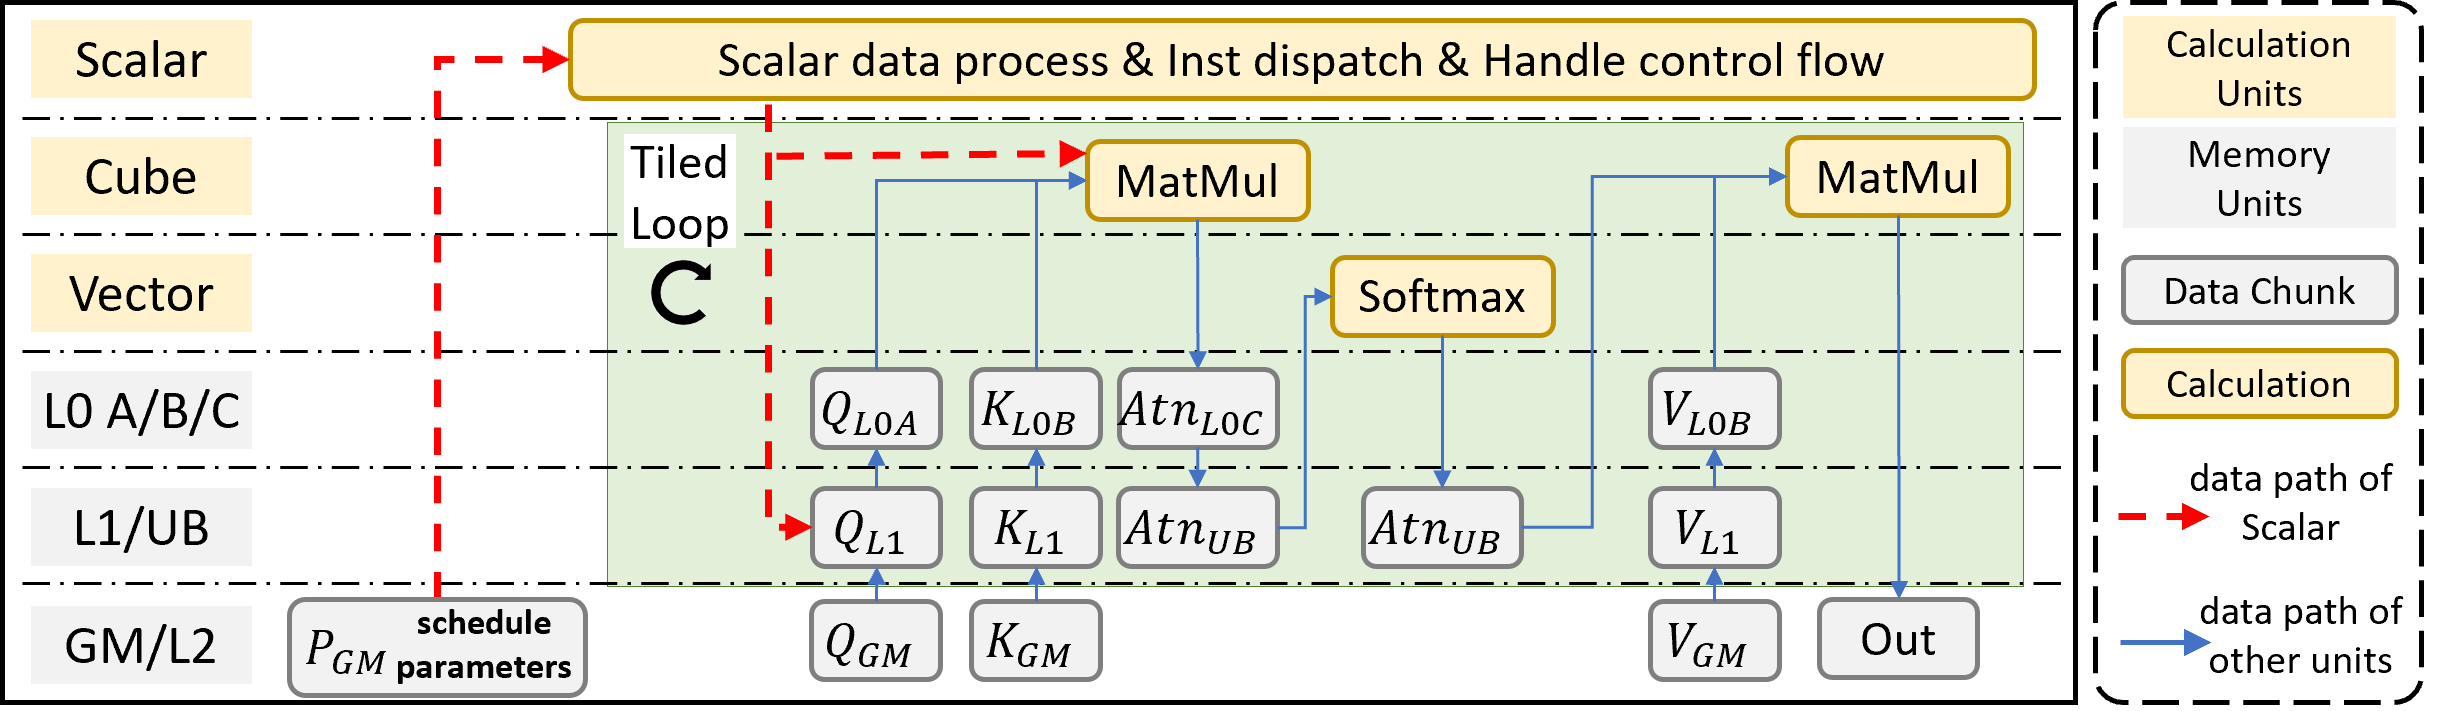
\includegraphics[width=0.8\textwidth]{figures/motivation/ascend-data-path.png}
%DIFDELCMD <   \caption{Execution flow of Flash Attention kernel \texttt{kernel\_fa} on the Ascend architecture.
%DIFDELCMD <   The \textbf{Scalar} unit acts as the central scheduler. 
%DIFDELCMD <   It continuously performs scalar calculations and dispatches instructions based on runtime parameters.
%DIFDELCMD <   The heavy scalar workload required by generic kernels may lead to a scalar bottleneck.}
%DIFDELCMD <   \Description{Diagram showing the interaction between Scalar, Cube, Vector, L1, and GM units on Ascend.}
%DIFDELCMD <   \label{fig:fa_on_ascend}
%DIFDELCMD <   \vspace{-10pt} 
%DIFDELCMD < \end{figure}
%DIFDELCMD < 

%DIFDELCMD < %%%
\DIFdel{In generic kernels, the Scalar unit may be over-occupied.
Since the Scalar unit typically possesses much lower computing power than a general-purpose host CPU, excessive scalar calculations related to schedule parameters can overload the unit.
Worse yet, excessive scalar intermediates may cause register spill, as there are only 32 general-purpose registers.
As a result, the powerful Cube and Vector units will stall to await instruction dispatch or scalar operands.
Furthermore, generic kernels often involve complex control flows (e.g., branching to handle different operator variants), which exerts heavy pressure on the instruction cache (I-Cache).
Frequent instruction jumps in such complex logic inevitably lead to I-Cache misses and pipeline flushes.
Finally, when loop bounds remain unknown at compile time, the compiler struggles to perform loop unrolling. 
Consequently, instruction scheduling is confined to the scope of a single iteration, preventing the effective overlapping of memory access and computation.
}%DIFDELCMD < 

%DIFDELCMD < %%%
\DIFdel{We further study this impact by profiling key operators from the }\textbf{\DIFdel{Qwen2.5-1.5B}} %DIFAUXCMD
\DIFdel{model on the Ascend NPU.
}\DIFdelend \DIFaddbegin \DIFadd{The representative profiles in }\DIFaddend \autoref{fig:perf_stats} \DIFdelbegin \DIFdel{presents the Scalar unit occupancy (the proportion of active cycles during kernel execution) and }\DIFdelend \DIFaddbegin \DIFadd{show high Scalar ratios and nonzero }\DIFaddend I-Cache miss rates \DIFdelbegin \DIFdel{.
The data reveals that the Scalar unit is active for 78\% to 91\% of total cycles, while I-Cache miss rates range from 3.1\% to 16.4\%}\DIFdelend \DIFaddbegin \DIFadd{for several of these kernels. These measurements motivate device-side specialization to reduce the scalar workload and improve instruction locality}\DIFaddend .

\DIFaddbegin \begin{figure}[htbp]
	\centering
	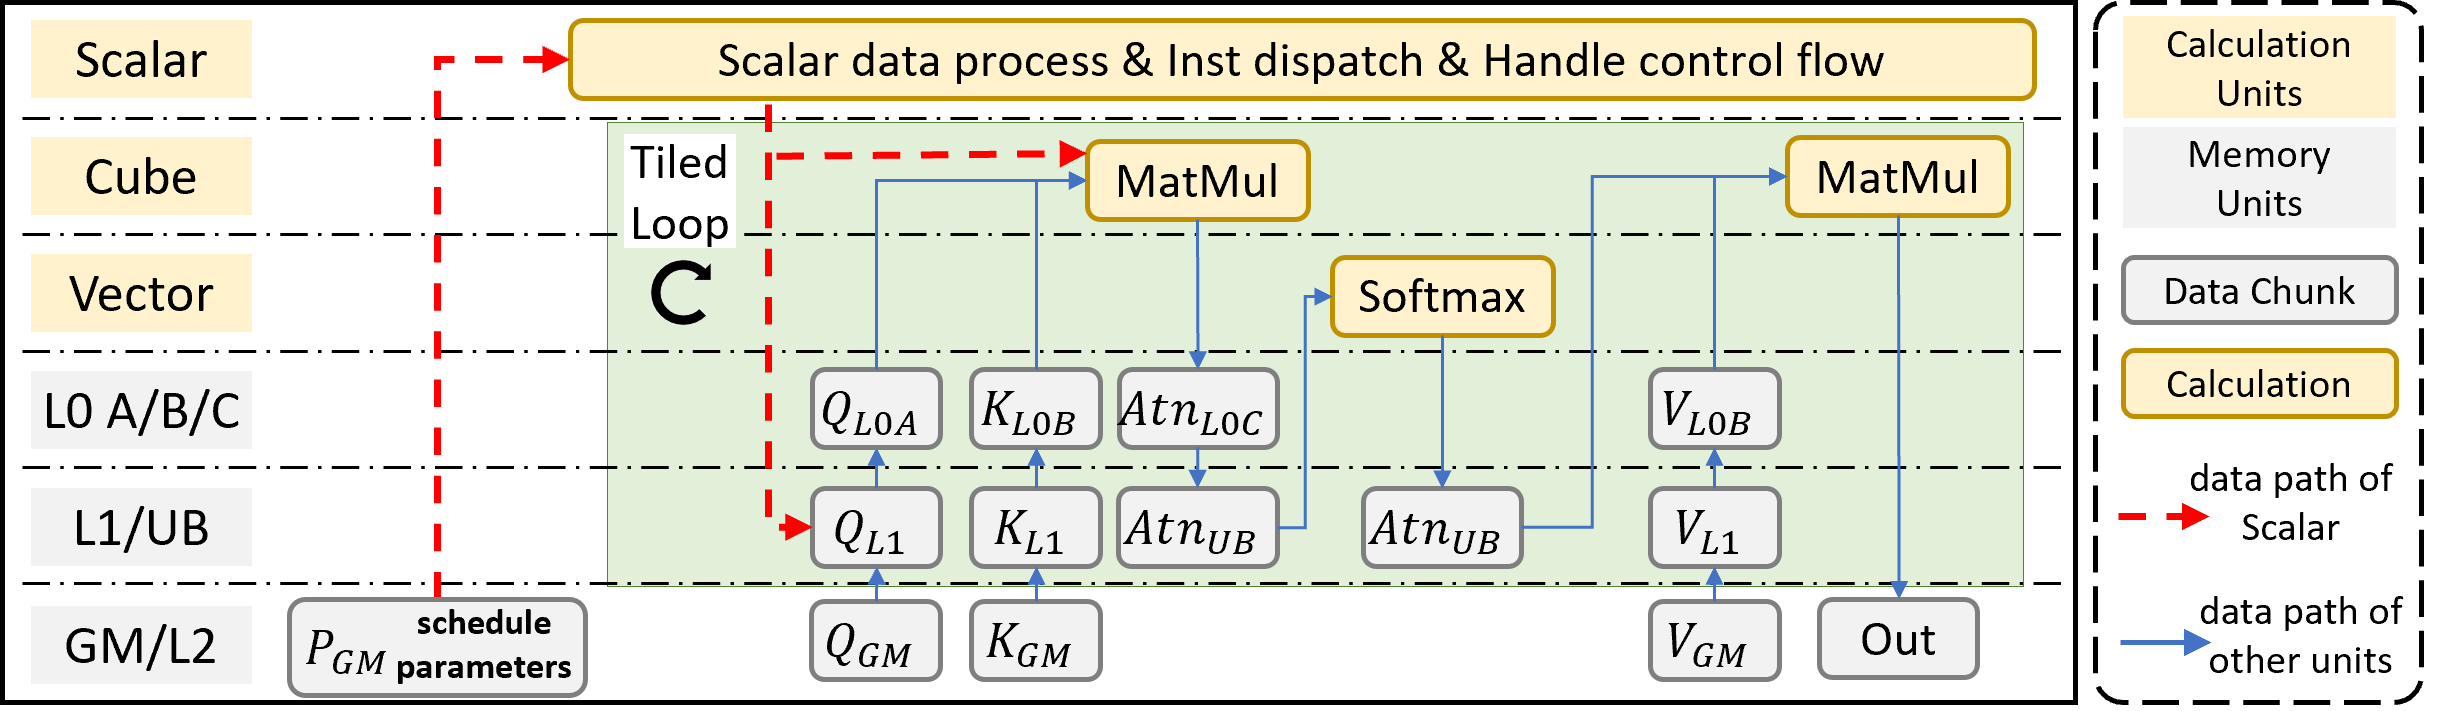
\includegraphics[width=0.8\textwidth]{figures/motivation/ascend-data-path.png}
	\caption{Execution flow of Flash Attention kernel \texttt{kernel\_fa} on the Ascend architecture.
		The \textbf{Scalar} unit acts as the central scheduler.
		It continuously performs scalar calculations and dispatches instructions based on runtime parameters.
		The heavy scalar workload required by generic kernels may lead to a scalar bottleneck.}
	\Description{Diagram showing the interaction between Scalar, Cube, Vector, L1, and GM units on Ascend.}
	\label{fig:fa_on_ascend}
	\vspace{-10pt}
\end{figure}

\DIFaddend \paragraph*{Code Bloat in \DIFdelbegin \DIFdel{Manually Specialized Libraries}\DIFdelend \DIFaddbegin \DIFadd{Schedule-Fixed Implementations}\DIFaddend .}
High-performance GPU libraries \DIFdelbegin \DIFdel{like }\DIFdelend \DIFaddbegin \DIFadd{such as }\DIFaddend FlashInfer~\cite{ye2025flashinfer} rely on C++ template metaprogramming to enable aggressive compiler optimizations.
To avoid runtime JIT overhead, \DIFdelbegin \DIFdel{these }\DIFdelend \DIFaddbegin \DIFadd{such }\DIFaddend libraries pre-instantiate kernels for the Cartesian product of all template parameters.
As described in \autoref{eq:flash_attention}, FA's configuration space includes head dimensions ($d_k \in \{64, 128, 256\}$), mask types, GQA sizes, and position encodings.
Combined with tile size configurations, this results in over 1000 binary instantiations, yet a specific model \DIFdelbegin \DIFdel{like }\textbf{\DIFdel{Qwen2-1.5B}} %DIFAUXCMD
\DIFdelend utilizes only $\sim$10 kernels.
This pre-instantiation strategy, while manageable on GPUs, is ill-suited for Ascend due to its more complex schedule parameters, forcing \DIFdelbegin \DIFdel{Ascend libraries }\DIFdelend \DIFaddbegin \DIFadd{their Ascend counterparts }\DIFaddend to rely on \DIFdelbegin \DIFdel{suboptimal generic kernels }\DIFdelend \DIFaddbegin \DIFadd{schedule-generic kernels with limited compile-time optimization}\DIFaddend .

\DIFdelbegin %DIFDELCMD < \begin{figure}[htbp]
%DIFDELCMD <   \centering
%DIFDELCMD <   \begin{minipage}{0.47\textwidth}
%DIFDELCMD <       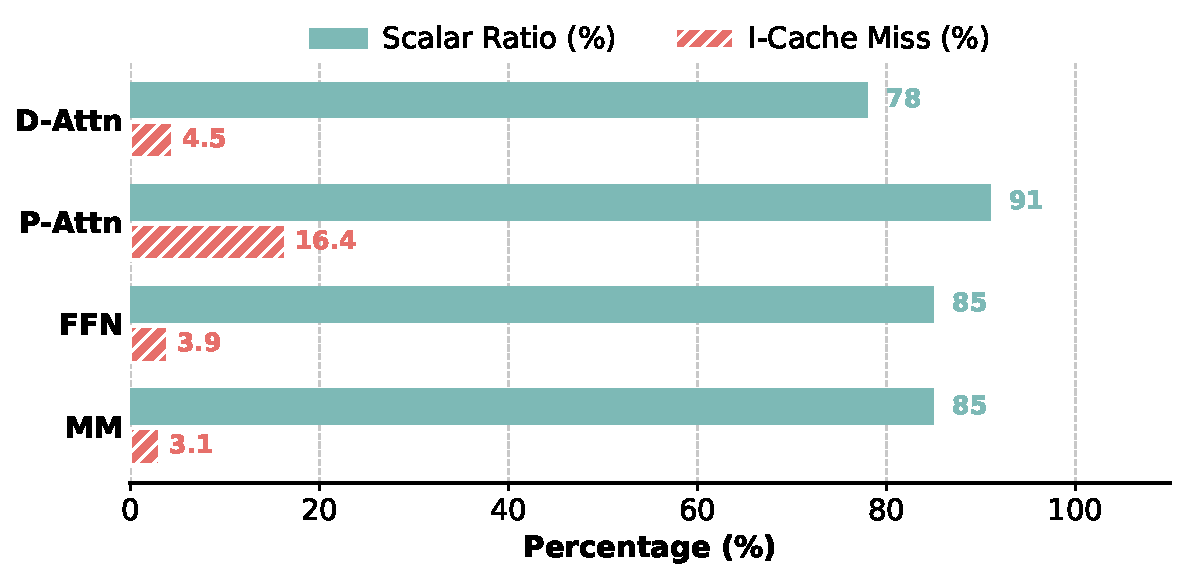
\includegraphics[width=\linewidth]{figures/motivation/metrics_analysis.pdf}
%DIFDELCMD <       \caption{Performance profiling of generic kernels. Lower is better for both metrics. Decoding Attention (\textbf{D-Attn}), Prefill Attention (\textbf{P-Attn}), Feed Forward Networks (\textbf{FFN}), and MatMul (\textbf{MM}).}
%DIFDELCMD <       \Description{Bar chart showing scalar instruction ratio and I-Cache miss rate for different operators.}
%DIFDELCMD <       \label{fig:perf_stats}
%DIFDELCMD <       \vspace{-10pt}
%DIFDELCMD <   \end{minipage}
%DIFDELCMD <   \hfill
%DIFDELCMD <   \begin{minipage}{0.47\textwidth}
%DIFDELCMD <       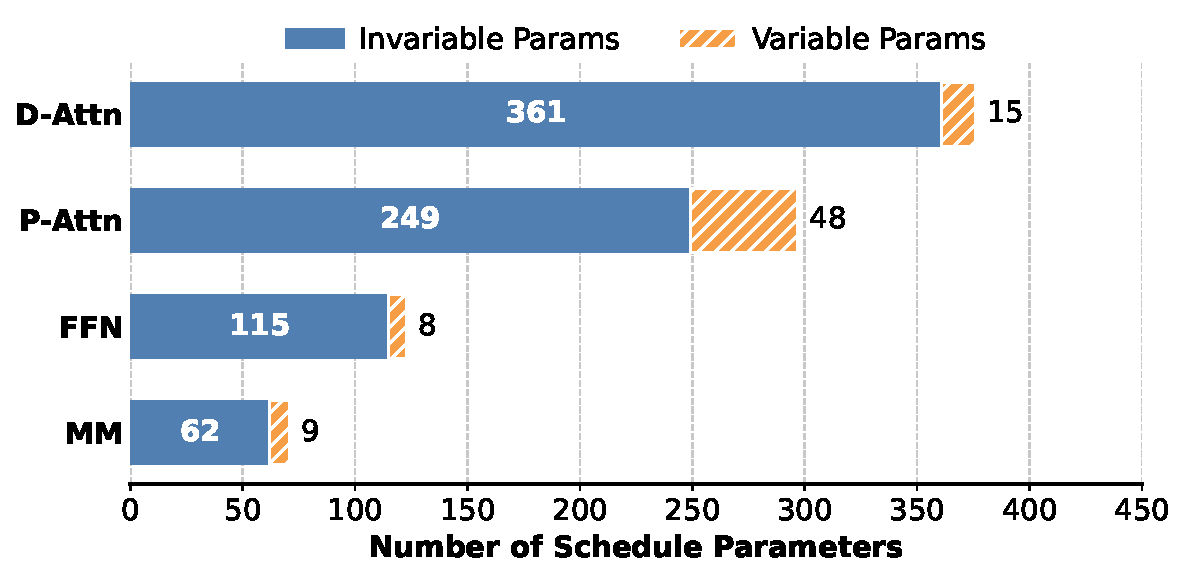
\includegraphics[width=\linewidth]{figures/motivation/parameter_breakdown.pdf}
%DIFDELCMD <       \caption{Number of schedule parameters of representative kernels. The vast majority are runtime invariants (Invariable Params), validating the potential for specialization.}
%DIFDELCMD <       \Description{Bar chart showing breakdown of kernel parameters into variable and invariable categories.}
%DIFDELCMD <       \label{fig:param_stats}
%DIFDELCMD <       \vspace{-10pt}
%DIFDELCMD <   \end{minipage}
%DIFDELCMD < \end{figure}
%DIFDELCMD < %%%
\DIFdelend \DIFaddbegin \begin{figure}[htbp]
	\centering
	\begin{minipage}{0.47\textwidth}
		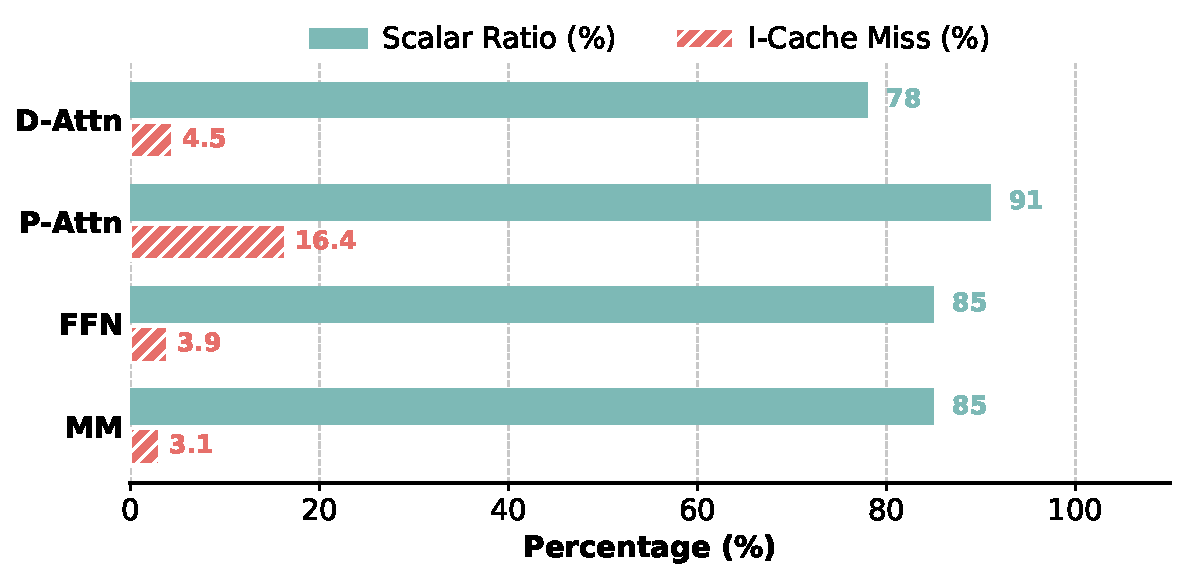
\includegraphics[width=\linewidth]{figures/motivation/metrics_analysis.pdf}
		\caption{Performance profiles of schedule-generic kernels, where lower values are better for both metrics: Decoding Attention (\textbf{D-Attn}), Prefill Attention (\textbf{P-Attn}), Feed Forward Networks (\textbf{FFN}), and MatMul (\textbf{MM}).}
		\Description{Bar chart showing scalar instruction ratio and I-Cache miss rate for different operators.}
		\label{fig:perf_stats}
	\end{minipage}
	\hfill
	\begin{minipage}{0.47\textwidth}
		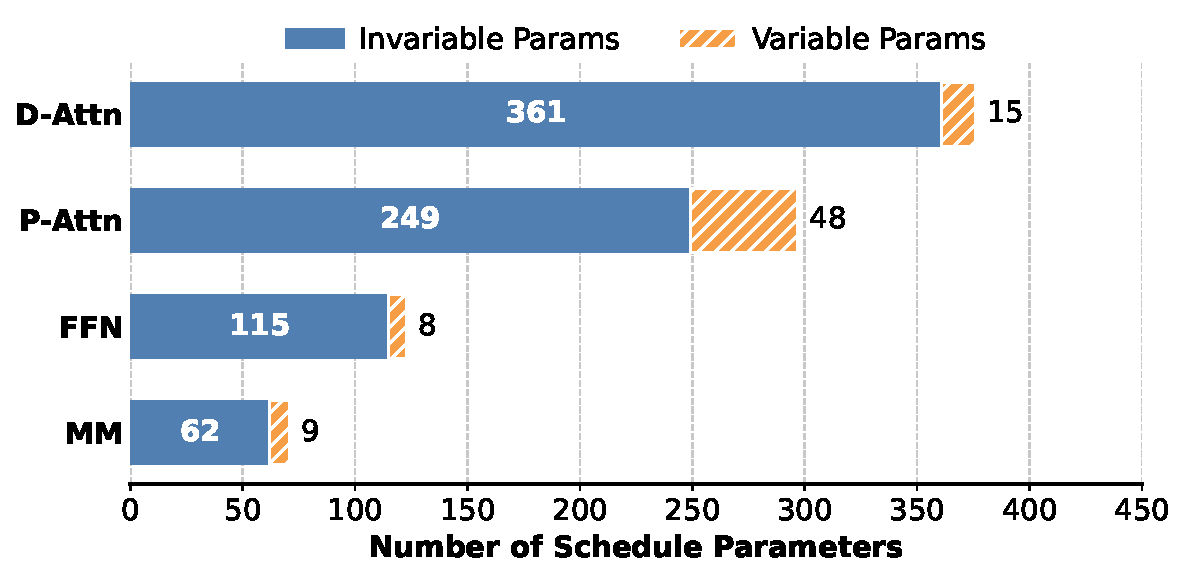
\includegraphics[width=\linewidth]{figures/motivation/parameter_breakdown.pdf}
		\caption{Number of schedule parameters of representative kernels. The vast majority are runtime invariants (Invariable Params), validating the potential for specialization.}
		\Description{Bar chart showing the breakdown of schedule parameters into variable and invariable categories.}
		\label{fig:param_stats}
	\end{minipage}
\end{figure}
\DIFaddend 

\subsubsection{Why Is Automatic \DIFdelbegin \DIFdel{Kernel }\DIFdelend \DIFaddbegin \DIFadd{Model-Specific }\DIFaddend Specialization Beneficial?}

We further analyze the schedule parameters of key operators from the \textbf{Qwen2.5-1.5B} model, classifying them into \textit{invariable parameters} (constants derived from model configuration) and \textit{variable parameters} (runtime-dependent values such as batch size and sequence length).
\autoref{fig:param_stats} reveals that the overwhelming majority of kernel parameters are invariable.
Propagating model-specific constants to resolve schedule parameters at compile time yields two benefits: (1) for \DIFdelbegin \DIFdel{generic kernels}\DIFdelend \DIFaddbegin \DIFadd{schedule-generic implementations}\DIFaddend , it enables model-specific \DIFaddbegin \DIFadd{kernel }\DIFaddend specialization with aggressive constant folding, reducing scalar overhead and I-Cache misses; (2) for \DIFdelbegin \DIFdel{manually specialized libraries}\DIFdelend \DIFaddbegin \DIFadd{schedule-fixed implementations}\DIFaddend , it makes kernel dispatch paths deterministic, enabling precise pruning of unused binaries.

\DIFaddbegin \DIFadd{Besides, the further sensitivity study in \S\ref{sec:eval:sensitivity} analyzes which schedule parameters tend to have the most significant impact on performance.
It reveals that a small subset of parameters, which lie in the hot path of the kernel, are responsible for the majority of performance impact.
}

\DIFaddend \subsection{Challenges and Design Insights}
\label{sec:motivation:challenges}

Achieving automatic \DIFdelbegin \DIFdel{kernel specialization requires analyzing the value flow from Python down to }\DIFdelend \DIFaddbegin \DIFadd{model-specific specialization requires transferring graph-level facts into }\DIFaddend C++ \DIFdelbegin \DIFdel{, which presents two major challenges that cannot be properly }\DIFdelend \DIFaddbegin \DIFadd{compilation and preserving them through host-side control flow.
These steps present two challenges not directly }\DIFaddend addressed by existing static \DIFdelbegin \DIFdel{analysis}\DIFdelend \DIFaddbegin \DIFadd{analyses}\DIFaddend .

\subsubsection{Challenge 1: \DIFdelbegin \DIFdel{The cross-language semantic gap}\DIFdelend \DIFaddbegin \DIFadd{Reconstructing Cross-Language Calling Contexts}\DIFaddend .}

\DIFdelbegin \DIFdel{Achieving automatic kernel specialization requires reconstructing the calling context for }\DIFdelend \DIFaddbegin \DIFadd{The first challenge is the Python/}\DIFaddend C++ \DIFdelbegin \DIFdel{operator functions, i.e., determining the tensor shapes and operator attribute values.
As shown in }%DIFDELCMD < \autoref{fig:motivating-example}%%%
\DIFdel{, these values are instantiated on the Python side and passed through the FFI layer to }\DIFdelend \DIFaddbegin \DIFadd{semantic gap: Graph IR constants and symbolic dimensions must be mapped to the memory states of their underlying C++ objects before LLVM can use them as compile-time facts.
This mapping is not a direct binding between arguments of graph IR node and }\DIFaddend C++ \DIFdelbegin \DIFdel{.
However, reconstructing this cross-language value flow faces significant challenges}\DIFdelend \DIFaddbegin \DIFadd{parameters.
Graph IR records typed values and shapes, whereas composite C++ parameters such as }\texttt{\DIFadd{Tensor}}\DIFadd{, }\texttt{\DIFadd{List}}\DIFadd{, and }\texttt{\DIFadd{Optional}} \DIFadd{use nested object layouts; after lowering, an access such as }\texttt{\DIFadd{query->size(1)}} \DIFadd{becomes pointer arithmetic and }\texttt{\DIFadd{load}} \DIFadd{instructions.
The analyzer must therefore reconstruct the corresponding base objects, pointers, field offsets, and field values, preserving concrete dimensions as constants and symbolic dimensions as unknown}\DIFaddend .

Existing cross-language \DIFdelbegin \DIFdel{analysis methods~\mbox{%DIFAUXCMD
\cite{kan2024taint4javac,Monat2021PythonC} }\hspace{0pt}%DIFAUXCMD
typically employ abstract interpretation at the FFI API level, modeling each }\DIFdelend \DIFaddbegin \DIFadd{analyses broadly follow two approaches: multilanguage abstract interpretation jointly analyzes programs on both sides of an FFI boundary~\mbox{%DIFAUXCMD
\cite{Monat2021PythonC}}\hspace{0pt}%DIFAUXCMD
, while specification-based methods summarize native behavior under a }\DIFaddend cross-language \DIFdelbegin \DIFdel{call as state transitions in an abstract domain.
While general-purpose, this approach is ill-suited for DL systems for two reasons.
First, the FFI layer contains substantial }\textit{\DIFdel{glue code}} %DIFAUXCMD
\DIFdel{for type conversions, dynamic dispatch}\DIFdelend \DIFaddbegin \DIFadd{caller context~\mbox{%DIFAUXCMD
\cite{kan2024taint4javac}}\hspace{0pt}%DIFAUXCMD
.
The former would have to traverse the Python Graph Executor and FFI glue for dispatch, type conversion, object construction}\DIFaddend , and reference counting, \DIFdelbegin \DIFdel{operations that are essential for language interoperability but irrelevant to the constant values we aim to extract.
Analyzing this glue code is both computationally expensive and unnecessary for our goal.
Second, the Python-side Graph Executor, which orchestrates operator invocations based on Graph IR , comprises complex logic spanning thousands of lines of code.
Performing full abstract interpretation over this codebase is prohibitively expensive.
These factors render traditional approaches impractical for reconstructing operator calling contexts in DL systems}\DIFdelend \DIFaddbegin \DIFadd{which is expensive and largely irrelevant to graph-level constants.
The latter assumes or derives a cross-language caller context but does not define how Graph IR metadata should materialize the field-sensitive C++ entry state required by LLVM}\DIFaddend .

\textit{Insight: \DIFdelbegin \DIFdel{Semantic modeling of core data types in DL systems}\DIFdelend \DIFaddbegin \DIFadd{Type-directed calling-context construction}\DIFaddend .}
\DIFdelbegin \DIFdel{Instead of analyzing FFI glue code and Python source code, we propose a cross-language semantic modeling approach grounded in two observations:
(1) }\textbf{\DIFdel{Finite and Stable Core Types:}} %DIFAUXCMD
\DIFdel{Data typesused for cross-language interaction in DL systems are highly convergent and stable (}\texttt{\DIFdel{Tensor}}%DIFAUXCMD
\DIFdelend \DIFaddbegin \DIFadd{DL operator interfaces use a limited set of parameter types}\DIFaddend , \DIFdelbegin \texttt{\DIFdel{Array}}%DIFAUXCMD
\DIFdel{, etc.), enabling comprehensive and precise semantic modeling.
(2) }\textbf{\DIFdel{Extract Constant Information from Graph IR:}} %DIFAUXCMD
\DIFdel{DL systems compile models and represent them using Graph IR (e.g., ATen IR), which contains precise information regarding operator input parameters, enabling direct extraction of semantic values without analyzing Python source code. Specifically, model-specific constants are captured as exact values from tracing, while dynamic dimensions are represented as symbolic variables.
Building on these insights, we directly map computation graph node information to the abstract states of C}\DIFdelend \DIFaddbegin \DIFadd{and their C}\DIFaddend ++ \DIFdelbegin \DIFdel{entry functions, achieving high-precision reconstruction of }\DIFdelend \DIFaddbegin \DIFadd{interface layouts are stable within a backend.
We can therefore define a context-update rule for each type and use Graph IR shapes and attributes to construct an accurate }\DIFaddend C++ \DIFdelbegin \DIFdel{contexts while avoiding the overhead of analyzing complex }\DIFdelend \DIFaddbegin \DIFadd{operator calling context directly.
This approach avoids analyzing }\DIFaddend FFI glue code\DIFaddbegin \DIFadd{; }\autoref{tab:semantic-rules} \DIFadd{formalizes the context-update rules used by }TilingInfer\DIFaddend .


\DIFdelbegin %DIFDELCMD < \begin{figure}[htbp]
%DIFDELCMD <   \noindent
%DIFDELCMD <   % --- 左侧 C++ 代码 ---
%DIFDELCMD <   

%DIFDELCMD <   \begin{minipage}{0.45\textwidth}
%DIFDELCMD <   \begin{lstlisting}[























%DIFDELCMD <   \end{lstlisting}
%DIFDELCMD <   \vspace{-15pt}
%DIFDELCMD <   \end{minipage}
%DIFDELCMD <   \hfill
%DIFDELCMD <   % --- 右侧 CFG 图 ---
%DIFDELCMD <   \begin{minipage}{0.5\textwidth}
%DIFDELCMD <     \centering
%DIFDELCMD <     \resizebox{\textwidth}{!}{%
%DIFDELCMD <     \begin{tikzpicture}[
%DIFDELCMD <         bb/.style={
%DIFDELCMD <             rectangle,
%DIFDELCMD <             rounded corners=5pt,
%DIFDELCMD <             draw=black,
%DIFDELCMD <             thick,
%DIFDELCMD <             minimum width=3.2cm,
%DIFDELCMD <             inner sep=6pt,
%DIFDELCMD <             font=\ttfamily\small,
%DIFDELCMD <             align=left
%DIFDELCMD <         },
%DIFDELCMD <         edge_label/.style={
%DIFDELCMD <             font=\ttfamily\small,
%DIFDELCMD <             midway
%DIFDELCMD <         },
%DIFDELCMD <         >=stealth
%DIFDELCMD <     ]
%DIFDELCMD <         % BB0: Entry
%DIFDELCMD <         \node[bb] (BB0) at (0, 0) {
%DIFDELCMD <           \textbf{BB0:}\\
%DIFDELCMD <           {\color{green!50!black}\%0} = call @check({\color{green!50!black}\%sq}, {\color{green!50!black}\%sk})\\
%DIFDELCMD <           {\color{green!50!black}\%1} = icmp ne {\color{green!50!black}\%0}, 0
%DIFDELCMD <         };
%DIFDELCMD <         

%DIFDELCMD <         % BB1: Error path
%DIFDELCMD <         \node[bb] (BB1) at (-2.2, -1.8) {
%DIFDELCMD <           \textbf{BB1:}\\
%DIFDELCMD <           call @print(...)
%DIFDELCMD <         };
%DIFDELCMD <         

%DIFDELCMD <         % BB2: Normal path
%DIFDELCMD <         \node[bb] (BB2) at (2.2, -1.8) {
%DIFDELCMD <           \textbf{BB2:}\\
%DIFDELCMD <           store 32, {\color{green!50!black}\%t}
%DIFDELCMD <         };
%DIFDELCMD <         

%DIFDELCMD <         % BB3: Exit
%DIFDELCMD <         \node[bb] (BB3) at (0, -4) {
%DIFDELCMD <           \textbf{BB3:}\\
%DIFDELCMD <           {\color{green!50!black}\%2} = phi [{\color{green!50!black}\%0}, {\color{green!50!black}\%BB1}], [0, {\color{green!50!black}\%BB2}]\\
%DIFDELCMD <           ret {\color{green!50!black}\%2}
%DIFDELCMD <         };
%DIFDELCMD <         

%DIFDELCMD <         % Edges
%DIFDELCMD <         \draw[->, thick] (BB0.south) -- (BB1.north)
%DIFDELCMD <           node[edge_label, left, pos=0.6] {{\color{green!50!black}$\%1$} (true)};
%DIFDELCMD <         \draw[->, thick] (BB0.south) -- (BB2.north)
%DIFDELCMD <           node[edge_label, right, pos=0.6] {$\neg${\color{green!50!black}$\%1$} (false)};
%DIFDELCMD <         \draw[->, thick] (BB1.south) -- (BB3.north);
%DIFDELCMD <         \draw[->, thick] (BB2.south) -- (BB3.north);
%DIFDELCMD <         

%DIFDELCMD <         % State annotations at convergence point
%DIFDELCMD <         \node[font=\ttfamily\fontsize{8pt}{9pt}\selectfont, align=center] at (-2.3, -2.8) {
%DIFDELCMD <           $*({\color{green!50!black}\%t}) = 0$\\
%DIFDELCMD <           {Error Path}
%DIFDELCMD <         };
%DIFDELCMD <         \node[font=\ttfamily\fontsize{8pt}{9pt}\selectfont, align=center] at (2.3, -2.8) {
%DIFDELCMD <           $*({\color{green!50!black}\%t}) = 32$\\
%DIFDELCMD <           {Normal Path}
%DIFDELCMD <         };
%DIFDELCMD <     \end{tikzpicture}
%DIFDELCMD <     }
%DIFDELCMD <     \caption{Control Flow Graph (CFG) of \texttt{set\_t}'s LLVM IR. Each node is a basic block containing LLVM IR instructions. Edges are labeled with branch conditions.}
%DIFDELCMD <     \label{fig:set_t_cfg}
%DIFDELCMD <     \vspace{-15pt}
%DIFDELCMD <   \end{minipage}
%DIFDELCMD <   \Description{Control flow graph showing early return path in LLVM IR.}
%DIFDELCMD < \end{figure}
%DIFDELCMD < %%%
\DIFdelend \DIFaddbegin \begin{figure}[htbp]
	\centering
	% --- left C++ code ---
	\begin{minipage}{0.39\textwidth}
		\begin{lstlisting}[
    language=C++,
    frame=single,
    caption={Early-exit path example.},
    basicstyle=\ttfamily\footnotesize,
    columns=fullflexible,
    framesep=1.5pt,
    aboveskip=0pt,
    belowskip=0pt,
    label={lst:early_return_code}
  ]
const status SUCCESS=0, ERROR=-1;
status check(int s1, int s2) {
  if(s1 != s2) return ERROR;
  return SUCCESS;
}
status set_t(int sk, int sv, int* t) {
  int e = check(sk, sv);
  if(e != SUCCESS) {
    print("error"); return e;
  }
  *t=32; // Tiling
  return SUCCESS;
}
  
\end{lstlisting}
	\end{minipage}
	\hspace{0.04\textwidth}
	% --- right CFG graph ---
	\begin{minipage}{0.47\textwidth}
		\centering
		\begin{tikzpicture}[
					bb/.style={
							rectangle,
							rounded corners=2.5pt,
							draw=black,
							thick,
							minimum width=2.5cm,
							inner sep=3pt,
							font=\ttfamily\footnotesize,
							align=left
						},
					edge_label/.style={
							font=\ttfamily\footnotesize,
							midway
						},
					>=stealth
				]
				% BB0: Entry
				\node[bb] (BB0) at (0, 0) {
				\textbf{BB0:}\\
				{\color{green!50!black}\%0} = call @check({\color{green!50!black}\%sk}, {\color{green!50!black}\%sv})\\
				{\color{green!50!black}\%1} = icmp ne {\color{green!50!black}\%0}, 0
				};

				% BB1: Early-exit path
				\node[bb] (BB1) at (-1.55, -1.2) {
					\textbf{BB1:}\\
					call @print(...)
				};

				% BB2: Normal path
				\node[bb] (BB2) at (1.55, -1.2) {
					\textbf{BB2:}\\
					store 32, {\color{green!50!black}\%t}
				};

				% BB3: Exit
				\node[bb] (BB3) at (0, -2.65) {
					\textbf{BB3:}\\
					{\color{green!50!black}\%2} = phi [{\color{green!50!black}\%0}, {\color{green!50!black}\%BB1}], [0, {\color{green!50!black}\%BB2}]\\
					ret {\color{green!50!black}\%2}
				};

				% Edges
				\draw[->, thick] (BB0.south) -- (BB1.north)
				node[edge_label, left, pos=0.6] {{\color{green!50!black}$\%1$} (true)};
				\draw[->, thick] (BB0.south) -- (BB2.north)
				node[edge_label, right, pos=0.6] {$\neg${\color{green!50!black}$\%1$} (false)};
				\draw[->, thick] (BB1.south) -- (BB3.north);
				\draw[->, thick] (BB2.south) -- (BB3.north);

				% State annotations at convergence point
				\node[font=\ttfamily\footnotesize, align=center] at (-1.6, -1.9) {
				$*({\color{green!50!black}\%t}) = 0$\\
				{Early-Exit Path}
				};
				\node[font=\ttfamily\footnotesize, align=center] at (1.6, -1.9) {
				$*({\color{green!50!black}\%t}) = 32$\\
				{Normal Path}
				};
		\end{tikzpicture}
		\caption{Control Flow Graph (CFG) of \texttt{set\_t}'s LLVM IR. Each node is a basic block containing LLVM IR instructions. Edges are labeled with branch conditions.}
		\label{fig:set_t_cfg}
	\end{minipage}
	\Description{Control flow graph showing an early-exit path in LLVM IR.}
\end{figure}
\DIFaddend 

\subsubsection{Challenge 2: Shape Checkers Leading to Early-Exit Paths}

\DIFaddbegin \DIFadd{The second challenge is preserving constant-propagation precision across shape-checker-induced early-exit paths without expensive path-sensitive analysis.
}\DIFaddend Operator libraries enforce \DIFdelbegin \DIFdel{shape constraints through runtime shape checkers to ensure }\DIFdelend \DIFaddbegin \DIFadd{constraints for }\DIFaddend memory safety and \DIFdelbegin \DIFdel{computational correctness.
As defined in }%DIFDELCMD < \autoref{eq:flash_attention}%%%
\DIFdel{, the Flash Attention operator imposes one constraint that the sequence lengths of $K$ and $V$ must be equal ($S_k = S_v$).
Violations of these constraints trigger early exits with error codes.
}%DIFDELCMD < 

%DIFDELCMD < \autoref{lst:early_return_code} %%%
\DIFdel{illustrates this pattern with a simplified example.
The function }\texttt{\DIFdel{check}} %DIFAUXCMD
\DIFdel{verifies whether two }\DIFdelend \DIFaddbegin \DIFadd{correctness; for example, Flash Attention requires equal key and value }\DIFaddend sequence lengths (\DIFdelbegin \DIFdel{denoted as }\texttt{\DIFdel{s1}} %DIFAUXCMD
\DIFdel{and }\texttt{\DIFdel{s2}}%DIFAUXCMD
\DIFdel{) match, returning }\texttt{\DIFdel{SUCCESS}} %DIFAUXCMD
\DIFdel{(0) if they are equal or }\texttt{\DIFdel{ERROR}} %DIFAUXCMD
\DIFdel{(-1)otherwise.
The function }\texttt{\DIFdel{set\_t}} %DIFAUXCMD
\DIFdel{uses this checker to validate the sequence lengths before computing the tiling parameter }\texttt{\DIFdel{t=32}}%DIFAUXCMD
\DIFdel{.
Since these dimensions are dynamic at compile time}\DIFdelend \DIFaddbegin \DIFadd{$S_k=S_v$).
Because these dimensions may remain symbolic}\DIFaddend , the compiler cannot \DIFdelbegin \DIFdel{determine whether the check will succeed or fail}\DIFdelend \DIFaddbegin \DIFadd{decide whether a check succeeds.
An early-exit path then bypasses assignments performed on the normal path, and merging the two states can obscure constants}\DIFaddend .

\DIFdelbegin %DIFDELCMD < \autoref{fig:set_t_cfg} %%%
\DIFdel{shows the corresponding CFG.
The entry block }\textbf{\DIFdel{BB0}} %DIFAUXCMD
\DIFdel{calls }\texttt{\DIFdel{@check}} %DIFAUXCMD
\DIFdel{and branches based on the result: the true branch leads to }\DIFdelend \DIFaddbegin \DIFadd{In }\autoref{lst:early_return_code}\DIFadd{, }\texttt{\DIFadd{check}} \DIFadd{returns }\texttt{\DIFadd{SUCCESS}} \DIFadd{or }\texttt{\DIFadd{ERROR}}\DIFadd{, and }\texttt{\DIFadd{set\_t}} \DIFadd{computes }\texttt{\DIFadd{t=32}} \DIFadd{only after the check succeeds.
The CFG in }\autoref{fig:set_t_cfg} \DIFadd{branches at }\textbf{\DIFadd{BB0}}\DIFadd{: }\DIFaddend \textbf{BB1} \DIFdelbegin \DIFdel{(error path ), while the false branch leads to }\DIFdelend \DIFaddbegin \DIFadd{returns through the early-exit path without defining }\texttt{\DIFadd{t}}\DIFadd{, whereas }\DIFaddend \textbf{BB2} \DIFdelbegin \DIFdel{(normal path) where }\texttt{\DIFdel{t=32}} %DIFAUXCMD
\DIFdel{is defined.
Both paths converge at }\DIFdelend \DIFaddbegin \DIFadd{defines it before both paths reach }\DIFaddend \textbf{BB3}.
\DIFdelbegin \DIFdel{At this merging site, standard path-insensitive analysis cannot determine whether the definition of }\DIFdelend \DIFaddbegin \DIFadd{If }\DIFaddend \texttt{t} \DIFdelbegin \DIFdel{originates from }\textbf{\DIFdel{BB2}} %DIFAUXCMD
\DIFdel{or is undefined from }\textbf{\DIFdel{BB1}}%DIFAUXCMD
\DIFdel{, resulting in a polluted abstract state $\{t \in \{0, 32\}\}$ that prevents constant propagation}\DIFdelend \DIFaddbegin \DIFadd{initially holds 0, path-insensitive merging yields $\{0,32\}$ rather than the normal-path constant 32.
Enumerating all paths would avoid this pollution, but nested shape checkers make full path-sensitive analysis impractical}\DIFaddend .

\textit{Insight: Conditional Return-Value Flow.}
\DIFdelbegin \DIFdel{The key to identifying early-exit paths lies in analyzing the relationship between path guards and the semantic meaning of return values.
Since shape checkers assign different constant values to the return variable on different execution paths (e.g., }\texttt{\DIFdel{SUCCESS}} %DIFAUXCMD
\DIFdel{on the normal path and }\texttt{\DIFdel{ERROR}} %DIFAUXCMD
\DIFdel{on the error path), we can determine whether a path is an early-exit by examining whether the path guard implies an error return value.
Specifically, we maintain path-sensitive guards and propagate them through the control flow.
If a path guard implies that the return value equals an error code, the path is identified as an early-exit path; otherwise, it is conservatively treated as a normal path.
During constant propagation, value states from confirmed early-exit paths are prevented from propagating to merge points, thereby avoiding state pollution.
In }%DIFDELCMD < \autoref{fig:set_t_cfg}%%%
\DIFdel{, the branch condition at }\DIFdelend \DIFaddbegin \DIFadd{CRVFG-based normal-path reasoning traces only the conditional flow of status return values and compares them with configured success and error sets.
In the example, the guard $\%1=(\%0\neq0)$ being true implies that }\texttt{\DIFadd{check}}\DIFadd{'s return value is not }\texttt{\DIFadd{SUCCESS}}\DIFadd{, so }\DIFaddend \textbf{BB0}\DIFdelbegin \DIFdel{is $\%1 = (\%0 \neq 0)$, where $\%0$ is the return value of }\texttt{\DIFdel{@check}}%DIFAUXCMD
\DIFdel{.
When the guard $\%1 = \texttt{true}$ holds, we have $\%0 \neq 0$, which implies $\%0 \neq \texttt{SUCCESS}$; hence the return value represents an error, and the path $\textbf{BB0} \rightarrow \textbf{BB1} \rightarrow \textbf{BB3}$ guarded by $\%1$ is an }\DIFdelend \DIFaddbegin \DIFadd{$\rightarrow$}\textbf{\DIFadd{BB1}} \DIFadd{is an }\DIFaddend early-exit \DIFdelbegin \DIFdel{path.
Conversely, when the guard $\neg\%1$ holds, we have $\%0 = 0 = \texttt{SUCCESS}$; hence the return value represents success, and the path $\textbf{BB0} \rightarrow \textbf{BB2} \rightarrow \textbf{BB3}$ guarded by $\neg\%1$ is a normal path.
%DIF <  \input{sections/motivation.tex}
 }\DIFdelend \DIFaddbegin \DIFadd{edge; its false branch is the normal edge.
Confirmed early-exit-edge states are excluded from normal-path merges, while unclassified edges are retained conservatively.
}

\end{comment}
\DIFaddend \section{System Design of TilingInfer}
\label{sec:design}

\DIFdelbegin %DIFDELCMD < \begin{figure}[htbp]
%DIFDELCMD <     \centering
%DIFDELCMD <     \resizebox{\linewidth}{!}{
%DIFDELCMD <     \colorlet{myblue}{blue!80!black}
%DIFDELCMD <     \begin{tikzpicture}[
%DIFDELCMD <         >=latex,
%DIFDELCMD <         thick,
%DIFDELCMD <         font=\sffamily\large,
%DIFDELCMD <         % 定义带折角的文档样式 (Document node style)
%DIFDELCMD <         doc/.style={
%DIFDELCMD <             rectangle, 
%DIFDELCMD <             minimum width=3.4cm, 
%DIFDELCMD <             minimum height=1.6cm,
%DIFDELCMD <             align=center, 
%DIFDELCMD <             inner sep=6pt,
%DIFDELCMD <             path picture={
%DIFDELCMD <                 \draw[thick]
%DIFDELCMD <                     (path picture bounding box.north west) --
%DIFDELCMD <                     (path picture bounding box.north east) --
%DIFDELCMD <                     ([yshift=0.35cm]path picture bounding box.south east) coordinate (SE1) --
%DIFDELCMD <                     ([xshift=-0.35cm]path picture bounding box.south east) coordinate (SE2) --
%DIFDELCMD <                     (path picture bounding box.south west) -- cycle;
%DIFDELCMD <                 \draw[thick]
%DIFDELCMD <                     (SE1) --
%DIFDELCMD <                     ([xshift=-0.35cm, yshift=0.35cm]path picture bounding box.south east) --
%DIFDELCMD <                     (SE2);
%DIFDELCMD <             }
%DIFDELCMD <         },
%DIFDELCMD <         % 定义标准矩形样式 (Standard box style)
%DIFDELCMD <         box/.style={
%DIFDELCMD <             rectangle, draw, thick, 
%DIFDELCMD <             minimum width=3.4cm, 
%DIFDELCMD <             minimum height=1.6cm,
%DIFDELCMD <             align=center, 
%DIFDELCMD <             inner sep=6pt
%DIFDELCMD <         },
%DIFDELCMD <         % 自定义蓝色
%DIFDELCMD <         myblue/.style={blue!80!black}
%DIFDELCMD <     ]
%DIFDELCMD < 

%DIFDELCMD <         % ====================
%DIFDELCMD <         % 第一排节点 (Row 1)
%DIFDELCMD <         % ====================
%DIFDELCMD <         

%DIFDELCMD <         % Node 1: Traced Graph IR
%DIFDELCMD <         % 增加 every node/.style={...} 阻断父节点的尺寸继承，防止图形变异
%DIFDELCMD <         \node[doc] (N1) at (0, 0) {
%DIFDELCMD <             Traced Graph IR\\[6pt]
%DIFDELCMD <             DAG: \tikz[baseline=-0.5ex, >=latex, every node/.style={minimum width=0pt, minimum height=0pt, inner sep=1pt}]{
%DIFDELCMD <                 \node[circle, draw, thick, myblue, minimum size=14pt] at (0,0) (c1) {};
%DIFDELCMD <                 \node[rectangle, draw, thick, myblue, rounded corners=1pt, minimum size=14pt, font=\small] at (1.1,0) (fa) {FA};
%DIFDELCMD <                 \node[circle, draw, thick, myblue, minimum size=14pt] at (2.2,0) (c2) {};
%DIFDELCMD <                 \draw[->, thick, myblue] (c1)--(fa);
%DIFDELCMD <                 \draw[->, thick, myblue] (fa)--(c2);
%DIFDELCMD <             }
%DIFDELCMD <         };
%DIFDELCMD < 

%DIFDELCMD <         % Node 2: Context Generation
%DIFDELCMD <         \node[box] (N2) at (5.6, 0) {Calling Context\\Generation\\[2pt](\S 3.2)};
%DIFDELCMD < 

%DIFDELCMD <         % Node 3: Calling Context
%DIFDELCMD <         \node[doc] (N3) at (10.2, 0) {Calling Context\\of LLVM IR\\Programs};
%DIFDELCMD < 

%DIFDELCMD <         % ====================
%DIFDELCMD <         % 第二排节点 (Row 2)
%DIFDELCMD <         % ====================
%DIFDELCMD <         

%DIFDELCMD <         % Node 4: C++ Implementation of Op
%DIFDELCMD <         \node[doc] (N4) at (0, -3.2) {
%DIFDELCMD <             C++ Implementation of Op\\[6pt]
%DIFDELCMD <             \tikz[baseline=-0.5ex, every node/.style={minimum width=0pt, minimum height=0pt}]{\node[draw, thick, gray!80!black, fill=gray!5, font=\normalsize, inner sep=6pt] {Built-in Shape Checkers};}
%DIFDELCMD <         };
%DIFDELCMD < 

%DIFDELCMD <         % Node 5: Early-Exit Identification
%DIFDELCMD <         \node[box] (N5) at (5.6, -3.2) {Early-Exit\\Identification\\[2pt](\S 3.3)};
%DIFDELCMD < 

%DIFDELCMD <         % Node 6: Early-Exit Edges
%DIFDELCMD <         \node[doc] (N6) at (10.2, -3.2) {Early-Exit\\Edges};
%DIFDELCMD < 

%DIFDELCMD <         % ====================
%DIFDELCMD <         % 右侧节点 (Right Side Nodes)
%DIFDELCMD <         % ====================
%DIFDELCMD <         

%DIFDELCMD <         % Node 7: Constant Propagation
%DIFDELCMD <         \node[box, minimum width=2.8cm] (N7) at (14.8, -1.6) {Constant\\Propagation\\[2pt](\S 3.4)};
%DIFDELCMD < 

%DIFDELCMD <         % Node 8: Kernel Specialization
%DIFDELCMD <         \node[box, minimum width=2.8cm] (N8) at (19.2, -1.6) {Kernel\\Specialization\\[2pt](\S 3.5)};
%DIFDELCMD < 

%DIFDELCMD <         % Node 9a & 9b: Code Bloat vs Performance (Two Dashed Circles)
%DIFDELCMD <         \node[circle, draw, thick, dashed, minimum size=1.4cm, align=center, inner sep=2pt] (N9a) at (17.8, -3.3) {
%DIFDELCMD <             \small Code Bloat
%DIFDELCMD <         };
%DIFDELCMD <         \node at (19.2, -3.3) {\textit{vs}};
%DIFDELCMD <         \node[circle, draw, thick, dashed, minimum size=1.4cm, align=center, inner sep=2pt] (N9b) at (20.6, -3.3) {
%DIFDELCMD <             \small Performance
%DIFDELCMD <         };
%DIFDELCMD < 

%DIFDELCMD <         % ====================
%DIFDELCMD <         % 连线 (Connections)
%DIFDELCMD <         % ====================
%DIFDELCMD <         

%DIFDELCMD <         % 上层直线 N1 -> N2 -> N3
%DIFDELCMD <         \draw[->] (N1) -- node[above, font=\itshape] {Op Info} (N2);
%DIFDELCMD <         \draw[->] (N2) -- (N3);
%DIFDELCMD < 

%DIFDELCMD <         % 下层直线 N1 -> N4 -> N5 -> N6
%DIFDELCMD <         \draw[->] (N1) -- node[right, font=\itshape] {bind} (N4);
%DIFDELCMD <         \draw[->] (N4) -- node[below, font=\itshape] {LLVM IR} (N5);
%DIFDELCMD <         \draw[->] (N5) -- (N6);
%DIFDELCMD < 

%DIFDELCMD <         % 右侧最后阶段连线 N7 -> N8
%DIFDELCMD <         \draw[->] (N7) -- (N8);
%DIFDELCMD < 

%DIFDELCMD <         % 复杂的总线汇集 (Bus merge to N7)
%DIFDELCMD <         \coordinate (merge_point) at (12.6, -1.6);           % 汇集点X坐标
%DIFDELCMD <         

%DIFDELCMD <         % 从 N3 延伸出来向下汇集的线
%DIFDELCMD <         \draw (N3.east) -| (merge_point);
%DIFDELCMD <         % 从 N6 延伸出来向上汇集的线
%DIFDELCMD <         \draw (N6.east) -| (merge_point);
%DIFDELCMD <         % 从汇集点直通 N7 的主轴线 (带箭头)
%DIFDELCMD <         \draw[->] (merge_point) -- (N7.west);
%DIFDELCMD <         

%DIFDELCMD <         % 从 N4 (C++ impls of Op) 到 N7 (Constant Propagation) 的连线
%DIFDELCMD <         \draw[->] (N4.east) -- ++(0.55,0) |- (N7);
%DIFDELCMD < 

%DIFDELCMD <     \end{tikzpicture}
%DIFDELCMD <     }
%DIFDELCMD <     \caption{The overall workflow of TilingInfer.}
%DIFDELCMD <     \Description{Flow diagram showing the workflow from Graph IR through Context Generation, Early-Exit Identification, Constant Propagation, to Kernel Specialization.}
%DIFDELCMD <     \label{fig:overall_workflow}
%DIFDELCMD <     \vspace{-10pt}
%DIFDELCMD < \end{figure}
%DIFDELCMD < %%%
\DIFdelend \DIFaddbegin \begin{figure}[htbp]
    \centering
    \resizebox{\linewidth}{!}{
    \colorlet{myblue}{blue!80!black}
    \begin{tikzpicture}[
        >=latex,
        thick,
        font=\sffamily\large,
        % 定义带折角的文档样式 (Document node style)
        doc/.style={
            rectangle, 
            minimum width=3.4cm, 
            minimum height=1.6cm,
            align=center, 
            inner sep=6pt,
            path picture={
                \draw[thick]
                    (path picture bounding box.north west) --
                    (path picture bounding box.north east) --
                    ([yshift=0.35cm]path picture bounding box.south east) coordinate (SE1) --
                    ([xshift=-0.35cm]path picture bounding box.south east) coordinate (SE2) --
                    (path picture bounding box.south west) -- cycle;
                \draw[thick]
                    (SE1) --
                    ([xshift=-0.35cm, yshift=0.35cm]path picture bounding box.south east) --
                    (SE2);
            }
        },
        % 定义标准矩形样式 (Standard box style)
        box/.style={
            rectangle, draw, thick, 
            minimum width=3.4cm, 
            minimum height=1.6cm,
            align=center, 
            inner sep=6pt
        },
        % 自定义蓝色
        myblue/.style={blue!80!black}
    ]

        % ====================
        % 第一排节点 (Row 1)
        % ====================

        % Node 1: Traced Graph IR
        % 增加 every node/.style={...} 阻断父节点的尺寸继承，防止图形变异
        \node[doc] (N1) at (0, 0) {
            Traced Graph IR\\[6pt]
            DAG: \tikz[baseline=-0.5ex, >=latex, every node/.style={minimum width=0pt, minimum height=0pt, inner sep=1pt}]{
                \node[circle, draw, thick, myblue, minimum size=14pt] at (0,0) (c1) {};
                \node[rectangle, draw, thick, myblue, rounded corners=1pt, minimum size=14pt, font=\small] at (1.1,0) (fa) {FA};
                \node[circle, draw, thick, myblue, minimum size=14pt] at (2.2,0) (c2) {};
                \draw[->, thick, myblue] (c1)--(fa);
                \draw[->, thick, myblue] (fa)--(c2);
            }
        };

        % Node 2: Context Generation
        \node[box] (N2) at (5.6, 0) {Calling Context\\Generation\\[2pt](\S 3.2)};

        % Node 3: Calling Context
        \node[doc] (N3) at (10.2, 0) {Calling Context\\of LLVM IR\\Programs};

        % ====================
        % 第二排节点 (Row 2)
        % ====================

        % Node 4: C++ Implementation of Op
        \node[doc] (N4) at (0, -3.2) {
            C++ Implementation of Op\\[6pt]
            \tikz[baseline=-0.5ex, every node/.style={minimum width=0pt, minimum height=0pt}]{\node[draw, thick, gray!80!black, fill=gray!5, font=\normalsize, inner sep=6pt] {Built-in Shape Checkers};}
        };

        % Node 5: Early-Exit Identification
        \node[box] (N5) at (5.6, -3.2) {Early-Exit\\Identification\\[2pt](\S 3.3)};

        % Node 6: Early-Exit Edges
        \node[doc] (N6) at (10.2, -3.2) {Early-Exit\\Edges};

        % ====================
        % 右侧节点 (Right Side Nodes)
        % ====================

        % Node 7: Constant Propagation
        \node[box, minimum width=2.8cm] (N7) at (14.8, -1.6) {Constant\\Propagation\\[2pt](\S 3.4)};

        % Node 8: Backend-specific use
        \node[box, minimum width=3.4cm] (N8) at (19.2, -1.6) {Backend-Specific\\Application\\[2pt](\S 3.5)};

        % Node 9a & 9b: distinct backend outcomes
        \node[box, dashed, minimum width=3.2cm, minimum height=1.1cm] (N9a) at (17.2, -3.7) {
            \small NPU Kernel\\[-1pt]\small Specialization
        };
        \node[box, dashed, minimum width=3.2cm, minimum height=1.1cm] (N9b) at (21.2, -3.7) {
            \small GPU Library\\[-1pt]\small Pruning
        };

        % ====================
        % 连线 (Connections)
        % ====================

        % 上层直线 N1 -> N2 -> N3
        \draw[->] (N1) -- node[above, font=\itshape] {Op Info} (N2);
        \draw[->] (N2) -- (N3);

        % 下层直线 N1 -> N4 -> N5 -> N6
        \draw[->] (N1) -- node[right, font=\itshape] {bind} (N4);
        \draw[->] (N4) -- node[below, font=\itshape] {LLVM IR} (N5);
        \draw[->] (N5) -- (N6);

        % 右侧最后阶段连线 N7 -> N8
        \draw[->] (N7) -- (N8);
        \draw[->] (N8.south) -- ++(0,-0.35) -| (N9a.north);
        \draw[->] (N8.south) -- ++(0,-0.35) -| (N9b.north);

        % 复杂的总线汇集 (Bus merge to N7)
        \coordinate (merge_point) at (12.6, -1.6);           % 汇集点X坐标

        % 从 N3 延伸出来向下汇集的线
        \draw (N3.east) -| (merge_point);
        % 从 N6 延伸出来向上汇集的线
        \draw (N6.east) -| (merge_point);
        % 从汇集点直通 N7 的主轴线 (带箭头)
        \draw[->] (merge_point) -- (N7.west);

        % 从 N4 (C++ impls of Op) 到 N7 (Constant Propagation) 的连线
        \draw[->] (N4.east) -- ++(0.55,0) |- (N7);

    \end{tikzpicture}
    }
    \caption{The overall workflow of TilingInfer.}
    \Description{Flow diagram showing Graph IR context generation, early-exit identification, constant propagation, NPU kernel specialization, and GPU library pruning.}
    \label{fig:overall_workflow}
\end{figure}
\DIFaddend 


\autoref{fig:overall_workflow} illustrates the workflow of TilingInfer.
\DIFaddbegin \DIFadd{Here, an }\emph{\DIFadd{early-exit edge}} \DIFadd{is the CFG edge that enters an early-exit path after a shape check fails.
}\DIFaddend The framework takes the traced Graph IR containing operator invocation information with model-specific constants as input, and proceeds through four stages: \textbf{Context Generation} (\S\ref{sec:design:context_construction}), \textbf{Early-Exit Identification} (\S\ref{sec:design:early-return}), \textbf{Constant Propagation} (\S\ref{sec:design:propagation}), and \textbf{Kernel Specialization} (\S\ref{sec:design:specialization}).
We detail each stage in the following subsections.

\DIFdelbegin %DIFDELCMD < \begin{table}[htbp]
%DIFDELCMD <   \centering
%DIFDELCMD <   \small
%DIFDELCMD <   \renewcommand{\arraystretch}{1.2}
%DIFDELCMD <   \setlength{\tabcolsep}{5pt} 
%DIFDELCMD <   \caption{Abstract domains and definitions in TilingInfer.}
%DIFDELCMD <   \label{fig:abstract-domain}
%DIFDELCMD <   \begin{tabular}{rl @{\hskip 0.8cm} rl}
%DIFDELCMD <     \toprule
%DIFDELCMD <     \textbf{Domain} & \textbf{Notation} & \textbf{Domain} & \textbf{Notation} \\
%DIFDELCMD <     \midrule
%DIFDELCMD <     % Row 1
%DIFDELCMD <     Top-level Variable & $v \in \mathcal{V}$ & 
%DIFDELCMD <     Constant Value & $c \in \mathbb{Z} \cup \mathbb{R} \cup \mathcal{F}$ \\
%DIFDELCMD <     

%DIFDELCMD <     % Row 2
%DIFDELCMD <     Base Object & $b \in \mathcal{B}$ & 
%DIFDELCMD <     Abstract Pointer & $p := \langle b, \hat{\delta} \rangle$ \\
%DIFDELCMD <     

%DIFDELCMD <     % Row 3 (左侧新增 Function Object)
%DIFDELCMD <     Function Object & $f \in \mathcal{F}$ & 
%DIFDELCMD <     Specialized Value & $sv := c~|~p~|~\top~|~\bot \in \mathcal{SV}$ \\
%DIFDELCMD <     

%DIFDELCMD <     % Row 4
%DIFDELCMD <     Concrete Offset & $\delta \in \mathbb{Z}$ & 
%DIFDELCMD <     Environment & $\mathbb{E} := \mathcal{V} \mapsto \mathcal{SV}$ \\
%DIFDELCMD <     

%DIFDELCMD <     % Row 5
%DIFDELCMD <     Abstract Offset & $\hat{\delta} \in \mathbb{Z} \cup \{ \bot \}$ & 
%DIFDELCMD <     Store & $\mathbb{S} := \mathcal{O} \mapsto \mathcal{SV}$ \\
%DIFDELCMD <     

%DIFDELCMD <     % Row 6 (现在两边都满了)
%DIFDELCMD <     Memory Location & $o := \langle b, \delta \rangle \in \mathcal{O}$ & 
%DIFDELCMD <     Calling Context & $\mathbb{C} := (\mathbb{E}, \mathbb{S})$ \\
%DIFDELCMD <     \bottomrule
%DIFDELCMD <   \end{tabular}
%DIFDELCMD <   \vspace{-15pt}
%DIFDELCMD < \end{table}
%DIFDELCMD < %%%
\DIFdelend \DIFaddbegin \begin{table}[htbp]
	\centering
	\small
	\renewcommand{\arraystretch}{1.05}
	\setlength{\tabcolsep}{5pt}
	\caption{Abstract domains and definitions in TilingInfer.}
	\label{fig:abstract-domain}
	\begin{tabular}{rl @{\hskip 0.8cm} rl}
		\toprule
		\textbf{Domain}    & \textbf{Notation}                                   & \textbf{Domain} & \textbf{Notation} \\
		\midrule
		% Row 1
		Top-level Variable & $v \in \mathcal{V}$                                 &
		Constant Value     & $c \in \mathbb{Z} \cup \mathbb{R} \cup \mathcal{F}$                                       \\

		% Row 2
		Base Object        & $b \in \mathcal{B}$                                 &
		Abstract Pointer   & $p := \langle b, \hat{\delta} \rangle$                                                    \\

		% Row 3 (左侧新增 Function Object)
		Function Object    & $f \in \mathcal{F}$                                 &
		Specialized Value  & $sv := c~|~p~|~\top~|~\bot \in \mathcal{SV}$                                              \\

		% Row 4
		Concrete Offset    & $\delta \in \mathbb{Z}$                             &
		Environment        & $\mathbb{E} := \mathcal{V} \mapsto \mathcal{SV}$                                          \\

		% Row 5
		Abstract Offset    & $\hat{\delta} \in \mathbb{Z} \cup \{ \bot \}$       &
		Store              & $\mathbb{S} := \mathcal{O} \mapsto \mathcal{SV}$                                          \\

		% Row 6 (现在两边都满了)
		Memory Location    & $o := \langle b, \delta \rangle \in \mathcal{O}$    &
		Calling Context    & $\mathbb{C} := (\mathbb{E}, \mathbb{S})$                                                  \\
			\bottomrule
		\end{tabular}
\end{table}
\DIFaddend 

\subsection{Definitions}\label{sec:design:definitions}

To formally describe the analysis of TilingInfer, we first define the abstract domains and notations used in our framework, as summarized in \autoref{fig:abstract-domain}.

\textit{Memory Model and Variables.}
We distinguish between SSA values and memory locations:
\begin{itemize}
	\item \kw{Top-level variables} ($v \in \mathcal{V}$) correspond to virtual registers in the LLVM IR.
	\item \kw{Base objects} ($b \in \mathcal{B}$) represent the abstract base addresses of memory blocks created at allocation sites (e.g., \texttt{alloca} instructions, global variables, or heap allocations).
	\item \kw{Memory locations} ($o \in \mathcal{O}$) represent specific fields within allocated objects. A location is defined as a pair $\langle b, \delta \rangle$, where $\delta \in \mathbb{Z}$ denotes a concrete byte offset relative to the base address $b$.
\end{itemize}

\textit{Abstract Values and Lattice.}
The analysis tracks the state of variables using \kw{Specialized Values} ($sv \in \mathcal{SV}$). The domain $\mathcal{SV}$ forms a lattice comprising the following elements:
\begin{itemize}
	\item \kw{Top ($\top$) and Bottom ($\bot$):} $\top$ represents an \textit{undefined} or \textit{uninitialized} state (the lattice top, indicating no information), while $\bot$ represents a generic \textit{variable} state where the value cannot be statically determined (the lattice bottom, indicating over-approximation).
	\item \kw{Concrete Constants ($c$):} These represent precise, known values. This category includes integers ($\in \mathbb{Z}$), floating-point numbers ($\in \mathbb{R}$), and \kw{Function Objects} ($f \in \mathcal{F}$), which represent references to functions targeted by direct or indirect calls.
	\item \kw{Abstract Pointers ($p$):} Defined structurally as $\langle b, \hat{\delta} \rangle$. A pointer $p$ represents an address computed by adding an \kw{Abstract Offset} $\hat{\delta}$ to a base object $b$. Here, $\hat{\delta} \in \mathbb{Z} \cup \{\bot\}$ allows the analysis to track precise offsets when possible, or degrade to $\bot$ if the offset is variable (e.g., a runtime index).
\end{itemize}

\textit{Context and State.}
The program state and \DIFdelbegin \DIFdel{inter-procedural }\DIFdelend \DIFaddbegin \DIFadd{interprocedural }\DIFaddend context are captured by the following mappings:
\begin{itemize}
	\item The \kw{Environment} $\mathbb{E}: \mathcal{V} \mapsto \mathcal{SV}$ maps top-level virtual registers to their abstract values.
	\item The \kw{Store} $\mathbb{S}: \mathcal{O} \mapsto \mathcal{SV}$ maps memory locations to the values stored therein. By mapping from pairs of $\langle b, \delta \rangle$, the store naturally supports field-sensitive tracking of structure fields and array elements.
	\item The \kw{Calling Context}~$\mathbb{C} := (\mathbb{E}, \mathbb{S})$ encapsulates the analysis state (environment and store) at the entry basic block of the current function. This context is determined by the caller and propagates constraints across \DIFdelbegin \DIFdel{functions during inter-procedural }\DIFdelend \DIFaddbegin \DIFadd{function boundaries during interprocedural }\DIFaddend analysis.
\end{itemize}

\DIFdelbegin %DIFDELCMD < \begin{figure}[htbp]
%DIFDELCMD < \centering
%DIFDELCMD < \begin{tikzpicture}[
%DIFDELCMD <     >=latex,
%DIFDELCMD <     thick,
%DIFDELCMD <     font=\sffamily\small,
%DIFDELCMD <     % 定义带折角的文档样式 (Document node style for data)
%DIFDELCMD <     doc/.style={
%DIFDELCMD <         rectangle, 
%DIFDELCMD <         minimum width=2.2cm, 
%DIFDELCMD <         minimum height=1.2cm,
%DIFDELCMD <         align=center, 
%DIFDELCMD <         inner sep=4pt,
%DIFDELCMD <         path picture={
%DIFDELCMD <             \draw[thick]
%DIFDELCMD <                 (path picture bounding box.north west) --
%DIFDELCMD <                 (path picture bounding box.north east) --
%DIFDELCMD <                 ([yshift=0.25cm]path picture bounding box.south east) coordinate (SE1) --
%DIFDELCMD <                 ([xshift=-0.25cm]path picture bounding box.south east) coordinate (SE2) --
%DIFDELCMD <                 (path picture bounding box.south west) -- cycle;
%DIFDELCMD <             \draw[thick]
%DIFDELCMD <                 (SE1) --
%DIFDELCMD <                 ([xshift=-0.25cm, yshift=0.25cm]path picture bounding box.south east) --
%DIFDELCMD <                 (SE2);
%DIFDELCMD <         }
%DIFDELCMD <     },
%DIFDELCMD <     % 定义标准矩形样式 (Standard box style for process)
%DIFDELCMD <     box/.style={
%DIFDELCMD <         rectangle, draw, thick, 
%DIFDELCMD <         minimum width=2.2cm, 
%DIFDELCMD <         minimum height=1.2cm,
%DIFDELCMD <         align=center, 
%DIFDELCMD <         inner sep=4pt
%DIFDELCMD <     },
%DIFDELCMD <     % 规则框样式
%DIFDELCMD <     rulebox/.style={
%DIFDELCMD <         rectangle, draw, thick, 
%DIFDELCMD <         dashed,
%DIFDELCMD <         minimum width=1.8cm, 
%DIFDELCMD <         minimum height=0.9cm,
%DIFDELCMD <         align=center, 
%DIFDELCMD <         inner sep=3pt
%DIFDELCMD <     }
%DIFDELCMD < ]
%DIFDELCMD < 

%DIFDELCMD <     % 1. Input Data (doc style)
%DIFDELCMD <     \node[doc] (input) at (0, 0) {{\small\ding{172}} Graph IR\\Node $N$};
%DIFDELCMD < 

%DIFDELCMD <     % 2. Process: Extract Parameter Types (box style)
%DIFDELCMD <     \node[box] (extract) at (3.2, 0) {{\small\ding{173}} Extract\\Param Types};
%DIFDELCMD < 

%DIFDELCMD <     % 3. Intermediate Data: Parameter Type Sequence Phi (doc style)
%DIFDELCMD <     \node[doc, minimum width=2.6cm] (param_types) at (6.6, 0) {{\small\ding{174}} Param Types $\Phi$\\$=[\phi_0, \dots, \phi_n]$};
%DIFDELCMD < 

%DIFDELCMD <     % 4. Process: Update Context (box style)
%DIFDELCMD <     \node[box, minimum width=2.8cm] (update) at (10.2, 0) {{\small\ding{175}} Update Context\\$\mathbb{C}_{i+1}{=}\mathcal{R}_{\phi_i}(\mathbb{C}_{i})$};
%DIFDELCMD < 

%DIFDELCMD <     % Side Inputs for Update Process (both above)
%DIFDELCMD <     \node[doc, minimum width=2.2cm, minimum height=0.9cm] (empty_ctx) at (8.6, 1.5) {{\small\ding{176}} Empty $\mathbb{C}_0$};
%DIFDELCMD <     

%DIFDELCMD <     \node[rulebox, minimum width=2.2cm] (rules) at (11.8, 1.5) {{\small\ding{177}} Rules $\mathcal{R}$};
%DIFDELCMD < 

%DIFDELCMD <     % 5. Final Output (doc style)
%DIFDELCMD <     \node[doc, minimum width=2.2cm] (output) at (13.8, 0) {{\small\ding{178}} Initial $\mathbb{C}_{init}$};
%DIFDELCMD < 

%DIFDELCMD <     % Edges
%DIFDELCMD <     \draw[->] (input) -- (extract);
%DIFDELCMD <     \draw[->] (extract) -- (param_types);
%DIFDELCMD <     \draw[->] (param_types) -- (update);
%DIFDELCMD <     \draw[->] (update) -- (output);
%DIFDELCMD <     

%DIFDELCMD <     % Side connections
%DIFDELCMD <     \draw[->] (empty_ctx) -- (update);
%DIFDELCMD <     \draw[->] (rules) -- (update);
%DIFDELCMD < 

%DIFDELCMD < \end{tikzpicture}
%DIFDELCMD < \caption{Workflow of Context Generation. \ding{172}-\ding{174}: Extraction phase; \ding{175}-\ding{178}: Context construction phase.}
%DIFDELCMD < \Description{Flow diagram showing the context generation process from Graph IR Node through Parameter Type Extraction to Call Context.}
%DIFDELCMD < \label{fig:context_workflow}
%DIFDELCMD < \vspace{-15pt}
%DIFDELCMD < \end{figure}
%DIFDELCMD < %%%
\DIFdelend \DIFaddbegin \begin{figure}[htbp]
\centering
\resizebox{\linewidth}{!}{%
\begin{tikzpicture}[
    >=latex,
    thick,
    font=\sffamily\small,
    % 定义带折角的文档样式 (Document node style for data)
    doc/.style={
        rectangle, 
        minimum width=2.2cm, 
        minimum height=1.2cm,
        align=center, 
        inner sep=4pt,
        path picture={
            \draw[thick]
                (path picture bounding box.north west) --
                (path picture bounding box.north east) --
                ([yshift=0.25cm]path picture bounding box.south east) coordinate (SE1) --
                ([xshift=-0.25cm]path picture bounding box.south east) coordinate (SE2) --
                (path picture bounding box.south west) -- cycle;
            \draw[thick]
                (SE1) --
                ([xshift=-0.25cm, yshift=0.25cm]path picture bounding box.south east) --
                (SE2);
        }
    },
    % 定义标准矩形样式 (Standard box style for process)
    box/.style={
        rectangle, draw, thick, 
        minimum width=2.2cm, 
        minimum height=1.2cm,
        align=center, 
        inner sep=4pt
    },
    % 规则框样式
    rulebox/.style={
        rectangle, draw, thick, 
        dashed,
        minimum width=1.8cm, 
        minimum height=0.9cm,
        align=center, 
        inner sep=3pt
    }
]

    % 1. Input Data (doc style)
    \node[doc] (input) at (0, 0) {{\small\ding{172}} Graph IR\\Node $N$};

    % 2. Process: Extract Metadata (box style)
    \node[box] (extract) at (3.2, 0) {{\small\ding{173}} Extract\\Metadata};

    % 3. Intermediate Data: Metadata Phi (doc style)
    \node[doc, minimum width=2.6cm] (metadata) at (6.6, 0) {{\small\ding{174}} Metadata $\Phi$\\$=[\phi_0, \dots, \phi_n]$};

    % 4. Process: Update Context (box style)
    \node[box, minimum width=2.8cm] (update) at (10.2, 0) {{\small\ding{175}} Update Context\\$\mathbb{C}_{i+1}{=}\mathcal{R}_{\phi_i}(\mathbb{C}_{i})$};

    % Side Inputs for Update Process (both above)
    \node[doc, minimum width=2.2cm, minimum height=0.9cm] (empty_ctx) at (8.6, 1.5) {{\small\ding{176}} Empty $\mathbb{C}_0$};

    \node[rulebox, minimum width=3.4cm] (rules) at (11.8, 1.5) {{\small\ding{177}} Type-directed\\context-update rules $\mathcal{R}$\\(\autoref{tab:semantic-rules})};

    % 5. Final Output (doc style)
    \node[doc, minimum width=2.2cm] (output) at (13.8, 0) {{\small\ding{178}} Initial $\mathbb{C}_{init}$};

    % Edges
    \draw[->] (input) -- (extract);
    \draw[->] (extract) -- (metadata);
    \draw[->] (metadata) -- (update);
    \draw[->] (update) -- (output);

    % Side connections
    \draw[->] (empty_ctx) -- (update);
    \draw[->] (rules) -- (update);

\end{tikzpicture}
}
\caption{Workflow of calling-context generation. \ding{172}--\ding{174}: extraction parses the Graph IR node into typed metadata $\Phi$. \ding{175}--\ding{178}: the five type-directed context-update rules $\mathcal{R}$ in \autoref{tab:semantic-rules} map $\Phi$ to the abstract C++ calling context $\mathbb{C}_{init}$.}
\Description{Flow diagram showing the context generation process from Graph IR Node through Metadata Extraction to Call Context.}
\label{fig:context_workflow}
\end{figure}
\DIFaddend 


\subsection{Calling Context Generation for C++}\label{sec:design:context_construction}

\autoref{fig:context_workflow} illustrates the overall workflow of context generation in TilingInfer.
The process takes a Graph IR node $N$ representing an operator invocation as input, and produces the initial calling context $\mathbb{C}_{init}$ for the corresponding C++ entry function.
This process bridges the \DIFdelbegin \DIFdel{semantic gap between the high-level Graph IR and the low-level }\DIFdelend \DIFaddbegin \DIFadd{representation and compilation boundary between Graph IR metadata and the abstract }\DIFaddend C++ \DIFdelbegin \DIFdel{execution state }\DIFdelend \DIFaddbegin \DIFadd{entry state required by LLVM analysis }\DIFaddend through two phases:
(1) \textbf{Extraction} (\ding{172}--\ding{174}), which parses the IR node $N$ to \DIFdelbegin \DIFdel{extract the parameter type information }\DIFdelend \DIFaddbegin \DIFadd{generate structured metadata }\DIFaddend $\Phi$; and
(2) \textbf{Construction} (\ding{175}--\ding{178}), which applies \DIFdelbegin \DIFdel{semantic rules }\DIFdelend \DIFaddbegin \DIFadd{the context-update rules $\mathcal{R}$ }\DIFaddend to transform the empty context $\mathbb{C}_0$ into the initial calling context $\mathbb{C}_{init}$.
\DIFaddbegin \DIFadd{Here, $\mathcal{R} = \{\mathcal{R}_{\textsc{Scalar}}, \mathcal{R}_{\textsc{String}}, \mathcal{R}_{\textsc{Tensor}}, \mathcal{R}_{\textsc{List}}, \mathcal{R}_{\textsc{Optional}}\}$ is the family of five type-directed context-update rules defined in }\autoref{tab:semantic-rules}\DIFadd{.
Each rule maps one typed metadata item to updates of the abstract environment and store, thereby materializing the C++ entry-state fields accessed by the target operator.
}\DIFaddend 

\subsubsection{Graph IR Node and \DIFdelbegin \DIFdel{Parameter Type }\DIFdelend \DIFaddbegin \DIFadd{Metadata }\DIFaddend Extraction}\label{sec:design:extract}

The Graph IR is a functional intermediate representation based on the ATen operator set, organized as a directed acyclic graph \DIFdelbegin \DIFdel{(DAG) }\DIFdelend where each node represents a logical ATen operator invocation.
We formally define a Graph IR node as:
\begin{equation}
	N = (\texttt{op}, \mathit{In}, \mathit{Out}, \sigma)
\end{equation}
where \texttt{op} is the ATen operator identifier (e.g., \texttt{aten.\DIFdelbegin \DIFdel{fa}\DIFdelend \DIFaddbegin \DIFadd{scaled\_dot\_product\_attention}\DIFaddend }\DIFaddbegin \DIFadd{, }\texttt{\DIFadd{aten.linear}}\DIFaddend ), $\mathit{In} = [x_1, \dots, x_m]$ is the ordered input list, $\mathit{Out} = [y_1, \dots, y_k]$ is the ordered output list, and $\sigma$ is the shape environment.
Each input $x_i$ is either a tensor \DIFdelbegin \DIFdel{(}\DIFdelend produced by another node \DIFdelbegin \DIFdel{) }\DIFdelend or an attribute\DIFdelbegin \DIFdel{(e.g., integer}\DIFdelend , \DIFdelbegin \DIFdel{float, arrays)}\DIFdelend \DIFaddbegin \DIFadd{such as an integer, a floating-point value, or an array.
The type of each input and output is directly represented by the corresponding metadata item $\phi_i$ in the context metadata $\Phi$, which is derived from the operator signature}\DIFaddend .
The shape environment $\sigma$ maps each tensor \DIFaddbegin \DIFadd{value }\DIFaddend $v$ to its type and shape information:
\begin{equation}
	\sigma(v) = (\texttt{dtype}(v), \texttt{shape}(v))
\end{equation}
where $\texttt{shape}(v) = [d_1, \dots, d_r]$ is a dimension list with each $d_i$ being either a concrete integer or a symbolic integer (\texttt{SymInt}) representing a runtime-determined dimension.
This design enables the Graph IR to capture dynamic shape information symbolically.

ATen operators have strictly defined signatures that specify the types of inputs and outputs.
\DIFdelbegin \DIFdel{To capture the type and value information of each parameter, we define the }\textit{\DIFdel{parameter type descriptor}} %DIFAUXCMD
\DIFdelend \DIFaddbegin \DIFadd{Each parameter type is directly mapped to a metadata variant }\DIFaddend $\phi$ \DIFdelbegin \DIFdel{as }\DIFdelend \DIFaddbegin \DIFadd{(e.g., }\textsc{\DIFadd{Tensor}}\DIFadd{, }\textsc{\DIFadd{Scalar}}\DIFadd{, }\textsc{\DIFadd{List}}\DIFadd{, }\textsc{\DIFadd{Optional}}\DIFadd{) without introducing a separate type variable.
}

TilingInfer \DIFadd{extracts }\ding{173} \DIFadd{the }\textit{\DIFadd{context metadata}} \DIFadd{$\Phi$ }\ding{174} \DIFadd{by aligning the Graph IR node's arguments with the operator's formal parameters.
For each parameter in the signature, if an explicit argument is provided, }TilingInfer \DIFadd{captures its value or shape information as a metadata item $\phi_i$ according to the parameter's type; if the argument is omitted and a default value exists, the default is used.
}

\DIFadd{The context metadata $\Phi = [\phi_0, \phi_1, \dots, \phi_n]$ is a sequence where each $\phi_i$ is }\DIFaddend a tagged union \DIFdelbegin \DIFdel{:
}\DIFdelend \DIFaddbegin \DIFadd{capturing the type and value information:
}\DIFaddend \begin{equation}
  \phi ::= \textsc{Scalar}(c) \mid \textsc{String}(s) \mid \textsc{Tensor}(\vec{d}) \mid \textsc{List}\langle\phi\DIFdelbegin \DIFdel{_1}\DIFdelend \DIFaddbegin \DIFadd{^{\prime}}\DIFaddend \rangle(\vec{e}) \mid \textsc{Optional}\langle\phi\DIFdelbegin \DIFdel{_1}\DIFdelend \DIFaddbegin \DIFadd{^{\prime}}\DIFaddend \rangle(v)
\end{equation}
Each parameter type constructor corresponds to the semantic meaning in the C++ operator interface:
\begin{itemize}
    \item $\textsc{Scalar}(c)$: Represents a scalar parameter of type \textsc{Int} or \textsc{Float}, where $c$ is the concrete value.
    \item $\textsc{String}(s)$: Represents a string parameter, where $s$ is the string content.
    \item $\textsc{Tensor}(\vec{d})$: Represents a tensor parameter, where $\vec{d} = [d_1, \dots, d_k]$ is the dimension list with each $d_i$ being either a concrete constant or a symbolic expression.
    \item \DIFdelbegin \DIFdel{$\textsc{List}\langle\phi_1\rangle(\vec{e})$}\DIFdelend \DIFaddbegin \DIFadd{$\textsc{List}\langle\phi^{\prime}\rangle(\vec{e})$}\DIFaddend : Represents a list parameter of element type \DIFdelbegin \DIFdel{$\phi_1$}\DIFdelend \DIFaddbegin \DIFadd{$\phi^{\prime}$}\DIFaddend , where $\vec{e}$ is the sequence of elements.
    \item \DIFdelbegin \DIFdel{$\textsc{Optional}\langle\phi_1\rangle(v)$}\DIFdelend \DIFaddbegin \DIFadd{$\textsc{Optional}\langle\phi^{\prime}\rangle(v)$}\DIFaddend : Represents an optional parameter, where $v$ is either a concrete value of type \DIFdelbegin \DIFdel{$\phi_1$ }\DIFdelend \DIFaddbegin \DIFadd{$\phi^{\prime}$ }\DIFaddend (present) or the special value $\text{None}$ (absent).
\end{itemize}


\DIFdelbegin %DIFDELCMD < TilingInfer %%%
\DIFdel{organizes the parameter type descriptors of a Graph IR node into a }\textit{\DIFdel{parameter type sequence}} %DIFAUXCMD
\DIFdel{$\Phi = [\phi_0, \phi_1, \dots, \phi_n]$.
	The extraction process }%DIFDELCMD < \ding{173}%%%
\DIFdel{--}%DIFDELCMD < \ding{174} %%%
\DIFdel{aligns the }\DIFdelend \DIFaddbegin \begin{example}
	\DIFadd{Consider the }\texttt{\DIFadd{aten.scaled\_dot\_product\_attention}} \DIFadd{invocation and the simplified C++ operator signature introduced in \mbox{%DIFAUXCMD
\cref{ex:sdpa-signature}}\hspace{0pt}%DIFAUXCMD
.
	The }\DIFaddend Graph IR node \DIFdelbegin \DIFdel{'s arguments with the operator's formal parameters: for each parameter in the signature }\DIFdelend \DIFaddbegin \DIFadd{is $N = (\texttt{aten.scaled\_dot\_product\_attention}, \mathit{In}, \mathit{Out}, \sigma)$, where $\mathit{In}=[\texttt{q},\texttt{k},\texttt{v},\texttt{None},0.0,1]$ follows the signature order, $\mathit{Out}=[\texttt{o}]$, and $1$ encodes }\texttt{\DIFadd{is\_causal=True}}\DIFadd{.
	The shape environment records:
	}\begin{align*}
		\DIFadd{\sigma(\texttt{q}) }& \DIFadd{= (\texttt{dtype}(\texttt{q}),}[\DIFadd{s_B,40,s_q,128}]\DIFadd{), }&
		\DIFadd{\sigma(\texttt{k}) }& \DIFadd{= (\texttt{dtype}(\texttt{k}),}[\DIFadd{s_B,8,s_{kv},128}]\DIFadd{), }\\
		\DIFadd{\sigma(\texttt{v}) }& \DIFadd{= (\texttt{dtype}(\texttt{v}),}[\DIFadd{s_B,8,s_{kv},128}]\DIFadd{), }&
		\DIFadd{\sigma(\texttt{o}) }& \DIFadd{= (\texttt{dtype}(\texttt{o}),}[\DIFadd{s_B,40,s_q,128}]\DIFadd{).
	}\end{align*}
	\DIFadd{Thus, $s_B$, $s_q$, and $s_{kv}$ remain symbolic, while 40}\DIFaddend , \DIFdelbegin \DIFdel{if an explicit argument is provided, }%DIFDELCMD < TilingInfer %%%
\DIFdel{captures its value or shape information as a parameter type descriptor $\phi_i$; if the argument is omitted and a default value exists, the default is used.
This parameter type sequence serves as the input for the subsequent Context Construction phase.
	}%DIFDELCMD < 

%DIFDELCMD < \begin{table}[htbp]
%DIFDELCMD <   \centering
%DIFDELCMD <   \caption{Context update rules for parameter types. C++ implementations are simplified to show only shape-related members.
%DIFDELCMD <   \textbf{Definitions:} $\ell$ denotes a base object. $\delta_{\texttt{field}}$ is the byte offset of a structure field. $\text{sz}_{\texttt{T}}$ is the size of type \texttt{T} in bytes.
%DIFDELCMD <   $\text{alloc}(\texttt{T})$ allocates a memory block sized for C++ type \texttt{T} and returns its base object.
%DIFDELCMD <   $\text{Process}(\phi_1, v, \ell)$ recursively populates the store at location $\ell$ with value $v$ of type $\phi_1$.
%DIFDELCMD <   $\alpha(x)$ returns $x$ if $x$ is concrete, or $\bot$ if symbolic.}
%DIFDELCMD <   \label{tab:semantic-rules}
%DIFDELCMD <   

%DIFDELCMD <   % 定义粗横线，使用 noalign 避免 booktabs 的间距问题
%DIFDELCMD <   \newcommand{\thickhline}{\noalign{\hrule}}
%DIFDELCMD <   

%DIFDELCMD <   \renewcommand{\arraystretch}{1.6}
%DIFDELCMD <   \small
%DIFDELCMD <   

%DIFDELCMD <   \begin{tabular}{m{0.20\textwidth}|m{0.26\textwidth}|>{\raggedright\arraybackslash}m{0.20\textwidth}|>{\raggedright\arraybackslash}m{0.26\textwidth}}
%DIFDELCMD <     \thickhline
%DIFDELCMD <     \textbf{Parameter Type} ($\phi$) & \textbf{C++ Implementations} & \textbf{Environment Update} & \textbf{Store Update} \\
%DIFDELCMD <     \hline
%DIFDELCMD <     

%DIFDELCMD <     % Row 1: Scalar
%DIFDELCMD <     $\textsc{Scalar}(c)$ &
%DIFDELCMD <     {\ttfamily int64\_t $c$; \newline double $c$;} &
%DIFDELCMD <     $v \mapsto \alpha(c)$ &
%DIFDELCMD <     None \\ \hline
%DIFDELCMD <     

%DIFDELCMD <     % Row 2: String
%DIFDELCMD <     $\textsc{String}(s)$ &
%DIFDELCMD <     {\ttfamily struct \{ \newline \hspace*{0.8em} size\_t len; \newline \hspace*{0.8em} char* data; \newline \}} &
%DIFDELCMD <     $\begin{aligned}
%DIFDELCMD <       & \ell = \text{alloc}(\texttt{str\_view}) \\
%DIFDELCMD <       & \ell_{buf} = \text{alloc}(\texttt{char}[|s|]) \\
%DIFDELCMD <       & v \mapsto \langle\ell, 0\rangle
%DIFDELCMD <     \end{aligned}$ &
%DIFDELCMD <     $\begin{aligned}
%DIFDELCMD <       & \langle \ell, \delta_{\texttt{len}} \rangle \mapsto |s| \\
%DIFDELCMD <       & \langle \ell, \delta_{\texttt{data}} \rangle \mapsto \langle\ell_{buf}, 0\rangle \\
%DIFDELCMD <       & \forall i.\; \langle \ell_{buf}, i \rangle \mapsto s[i]
%DIFDELCMD <     \end{aligned}$
%DIFDELCMD <     \\ \hline
%DIFDELCMD <     

%DIFDELCMD <     % Row 3: Tensor
%DIFDELCMD <     $\textsc{Tensor}(\vec{d})$ \newline $\vec{d}=[d_1 \dots d_k]$ &
%DIFDELCMD <     {\ttfamily struct \{ \newline \hspace*{0.8em} int* sizes; \newline \hspace*{0.8em} int ndim; \newline \}} &
%DIFDELCMD <     $\begin{aligned}
%DIFDELCMD <       & \ell = \text{alloc}(\texttt{Tensor}) \\
%DIFDELCMD <       & \ell_{sz} = \text{alloc}(\texttt{int}[k]) \\
%DIFDELCMD <       & v \mapsto \langle\ell, 0\rangle
%DIFDELCMD <     \end{aligned}$ &
%DIFDELCMD <     $\begin{aligned}
%DIFDELCMD <       & \langle \ell, \delta_{\texttt{ndim}} \rangle \mapsto k \\
%DIFDELCMD <       & \langle \ell, \delta_{\texttt{sizes}} \rangle \mapsto \langle\ell_{sz}, 0\rangle \\
%DIFDELCMD <       & \forall i.\; \langle \ell_{sz}, i \cdot \text{sz}_{\texttt{int}} \rangle \mapsto \alpha(d_i)
%DIFDELCMD <     \end{aligned}$
%DIFDELCMD <     \\ \hline
%DIFDELCMD <     

%DIFDELCMD <     % Row 4: List
%DIFDELCMD <     $\textsc{List}\langle\phi_1\rangle(\vec{e})$ \newline $\vec{e}=[e_1 \dots e_n]$ &
%DIFDELCMD <     {\ttfamily struct \{ \newline \hspace*{0.8em} size\_t size; \newline \hspace*{0.8em} T* data; \newline \}} &
%DIFDELCMD <     $\begin{aligned}
%DIFDELCMD <       & \ell = \text{alloc}(\texttt{List}\langle\phi_1\rangle) \\
%DIFDELCMD <       & \ell_{buf} = \text{alloc}(\phi_1[n]) \\
%DIFDELCMD <       & v \mapsto \langle\ell, 0\rangle
%DIFDELCMD <     \end{aligned}$ &
%DIFDELCMD <     $\begin{aligned}
%DIFDELCMD <       & \langle \ell, \delta_{\texttt{size}} \rangle \mapsto n \\
%DIFDELCMD <       & \langle \ell, \delta_{\texttt{data}}\rangle \mapsto \langle\ell_{buf}, 0\rangle \\
%DIFDELCMD <       & \forall i. \; \text{Process}(\phi_1, e_i, \langle \ell_{buf}, i \cdot \text{sz}_{\phi_1} \rangle)
%DIFDELCMD <     \end{aligned}$
%DIFDELCMD <     \\ \hline
%DIFDELCMD <     

%DIFDELCMD <     % Row 5: Optional
%DIFDELCMD <     $\textsc{Optional}\langle\phi_1\rangle(u)$ &
%DIFDELCMD <     {\ttfamily struct \{ \newline \hspace*{0.8em} bool has\_val; \newline \hspace*{0.8em} T* val; \newline \}} &
%DIFDELCMD <     $\begin{aligned}
%DIFDELCMD <       & \ell = \text{alloc}(\texttt{Optional}\langle\phi_1\rangle) \\
%DIFDELCMD <       & \text{if } u \neq \text{None}: \\
%DIFDELCMD <       & \quad \ell_{obj} = \text{alloc}(\phi_1) \\
%DIFDELCMD <       & v \mapsto \langle\ell, 0\rangle
%DIFDELCMD <     \end{aligned}$ &
%DIFDELCMD <     $\begin{aligned}
%DIFDELCMD <       & \langle \ell, \delta_{\texttt{has\_val}} \rangle \mapsto (u \neq \text{None}) \\
%DIFDELCMD <       & \text{if } u \neq \text{None}: \\
%DIFDELCMD <       & \quad \langle \ell, \delta_{\texttt{val}} \rangle \mapsto \langle\ell_{obj}, 0\rangle \\
%DIFDELCMD <       & \quad \text{Process}(\phi_1, u, \langle \ell_{obj}, 0 \rangle)
%DIFDELCMD <     \end{aligned}$
%DIFDELCMD <     \\
%DIFDELCMD <     \thickhline
%DIFDELCMD <   \end{tabular}
%DIFDELCMD <   \vspace{-10pt}
%DIFDELCMD < \end{table}
%DIFDELCMD < 

%DIFDELCMD < \begin{example}
%DIFDELCMD < %%%
\DIFdel{Consider the }\texttt{\DIFdel{aten.fa}} %DIFAUXCMD
\DIFdel{operator implementing the Flash Attention computation defined in }%DIFDELCMD < \autoref{eq:flash_attention}%%%
\DIFdel{:
}%DIFDELCMD < \begin{center}
%DIFDELCMD < %%%
\texttt{\DIFdel{aten.fa(Tensor q, Tensor k, Tensor v, int}%DIFDELCMD < []%%%
\DIFdel{? lens, int? mask\_type) -> Tensor}}
%DIFAUXCMD
%DIFDELCMD < \end{center}
%DIFDELCMD < %%%
\DIFdel{The Graph IR node $N = (\texttt{aten.fa}, \mathit{In}, \mathit{Out}, \sigma)$ where $\mathit{In}$ contains: query tensor $q$ of shape $[B, 40, S, 64]$ (with symbolic $B$, $S$ and concrete $h_q=40$, $d_k=64$), key tensor $k$ and value tensor $v$ both of shape $[B, 40, S, 64]$ (concrete $h_{kv}=40$), an optional sequence lengths array, and an omitted optional mask type (default }\texttt{\DIFdel{None}}%DIFAUXCMD
\DIFdel{)}\DIFdelend \DIFaddbegin \DIFadd{8, and 128 are concrete}\DIFaddend .
	The extracted \DIFdelbegin \DIFdel{parameter type sequence }\DIFdelend \DIFaddbegin \DIFadd{metadata }\DIFaddend $\Phi$ is:
	\begin{align*}
		\Phi = [ & \textsc{Tensor}([\DIFdelbegin \DIFdel{B}\DIFdelend \DIFaddbegin \DIFadd{s_B}\DIFaddend ,40,\DIFdelbegin \DIFdel{S}\DIFdelend \DIFaddbegin \DIFadd{s_q}\DIFaddend ,\DIFdelbegin \DIFdel{64}\DIFdelend \DIFaddbegin \DIFadd{128}\DIFaddend ]), \textsc{Tensor}([\DIFdelbegin \DIFdel{B}\DIFdelend \DIFaddbegin \DIFadd{s_B}\DIFaddend ,\DIFdelbegin \DIFdel{40}\DIFdelend \DIFaddbegin \DIFadd{8}\DIFaddend ,\DIFdelbegin \DIFdel{S}\DIFdelend \DIFaddbegin \DIFadd{s_{kv}}\DIFaddend ,\DIFdelbegin \DIFdel{64}\DIFdelend \DIFaddbegin \DIFadd{128}\DIFaddend ]), \\
		         & \textsc{Tensor}([\DIFdelbegin \DIFdel{B}\DIFdelend \DIFaddbegin \DIFadd{s_B}\DIFaddend ,\DIFdelbegin \DIFdel{40}\DIFdelend \DIFaddbegin \DIFadd{8}\DIFaddend ,\DIFdelbegin \DIFdel{S}\DIFdelend \DIFaddbegin \DIFadd{s_{kv}}\DIFaddend ,\DIFdelbegin \DIFdel{64}\DIFdelend \DIFaddbegin \DIFadd{128}\DIFaddend ]), \textsc{Optional}\langle\DIFdelbegin \textsc{\DIFdel{List}}%DIFAUXCMD
%DIFDELCMD < \langle%%%
\textsc{\DIFdel{Scalar}}%DIFAUXCMD
%DIFDELCMD < \rangle%%%
\DIFdelend \DIFaddbegin \textsc{\DIFadd{Tensor}}\DIFaddend \rangle(\text{None}), \\
		         & \DIFdelbegin \textsc{\DIFdel{Optional}}%DIFAUXCMD
%DIFDELCMD < \langle%%%
\textsc{\DIFdel{Scalar}}%DIFAUXCMD
%DIFDELCMD < \rangle%%%
\DIFdel{(\text{None})}\DIFdelend \DIFaddbegin \textsc{Scalar}(0.0)\DIFadd{, }\textsc{Scalar}(1) \DIFaddend ]\DIFaddbegin \DIFadd{.
	}\DIFaddend \end{align*}
\DIFdelbegin \DIFdel{Each parameter type descriptor $\phi_i$ directly captures the type and value of the corresponding $i$-th input.
For tensor parameters, the dimension list captures both concrete constants (e.g., $40$, $64$) derived from the model configuration and symbolic expressions (e.g., $B$, $S$) representing runtime-determined dimensions.
}\DIFdelend \end{example}

\subsubsection{Context Construction from \DIFdelbegin \DIFdel{Parameter Types}\DIFdelend \DIFaddbegin \DIFadd{Metadata}\DIFaddend }\label{sec:design:update}

The goal of the construction phase is to synthesize the initial C++ calling context $\mathbb{C}_{init} = (\mathbb{E}, \mathbb{S})$ from the \DIFdelbegin \DIFdel{parameter type sequence }\DIFdelend \DIFaddbegin \DIFadd{metadata }\DIFaddend $\Phi$.
Starting with an empty context $\mathbb{C}_{0}$ \ding{176}, TilingInfer iterates \DIFdelbegin \DIFdel{through each parameter type descriptor }\DIFdelend \DIFaddbegin \DIFadd{over the metadata items }\DIFaddend $\phi_i$ and sequentially updates \ding{175} the abstract state:
\DIFaddbegin \DIFadd{for $\tau_i = \operatorname{type}(\phi_i)$, we write $\mathcal{R}_{\phi_i}(\mathbb{C}) := \mathcal{R}_{\tau_i}(\mathbb{C}, \phi_i)$ for the instance of the matching type-directed context-update rule.
}\DIFaddend \begin{equation}
	\mathbb{C}_{init} = \mathcal{R}_{\phi_n} \circ \dots \circ \mathcal{R}_{\phi_1} \circ \mathcal{R}_{\phi_0} (\mathbb{C}_0)
\end{equation}
\DIFdelbegin \DIFdel{For each parameter type descriptor $\phi_i$, we apply a semantic modeling rule}\DIFdelend \DIFaddbegin \DIFadd{Thus, each }\DIFaddend $\mathcal{R}_{\phi_i}$ \DIFdelbegin %DIFDELCMD < \ding{177} %%%
\DIFdel{to transform }\DIFdelend \DIFaddbegin \DIFadd{in the equation is an application of exactly one of the five context-update rules in $\mathcal{R}$ shown in }\autoref{tab:semantic-rules}\DIFadd{, transforming }\DIFaddend the high-level \DIFdelbegin \DIFdel{parameter type }\DIFdelend \DIFaddbegin \DIFadd{metadata }\DIFaddend into the low-level memory representation.

\subsubsection{\DIFdelbegin \DIFdel{Update }\DIFdelend \DIFaddbegin \DIFadd{Context-Update }\DIFaddend Rules for \DIFdelbegin \DIFdel{Parameter }\DIFdelend \DIFaddbegin \DIFadd{Metadata }\DIFaddend Types}\label{sec:design:rules}

\autoref{tab:semantic-rules} presents the \DIFdelbegin \DIFdel{update rulesfor each parameter type.
}\DIFdelend \DIFaddbegin \DIFadd{five context-update rules, one for each supported metadata type.
}

\begin{table}[htbp]
  \centering
  \caption{The five type-directed context-update rules $\mathcal{R}$ for constructing the abstract C++ entry state.
  \textbf{Definitions:} $\text{alloc}(\texttt{T})$ creates an abstract base object with the validated fields accessed through type \texttt{T}.
  $\text{Process}(\mathit{type}, v, \ell)$ recursively populates the store at location $\ell$ with value $v$ of type $\mathit{type}$.
  $\alpha(x)$ returns $x$ if concrete, or $\bot$ if symbolic.}
  \label{tab:semantic-rules}

  % 定义粗横线，使用 noalign 避免 booktabs 的间距问题
  \newcommand{\thickhline}{\noalign{\hrule}}

  \renewcommand{\arraystretch}{1.5}
  \scriptsize

  \begin{tabular}{m{0.19\textwidth}|m{0.18\textwidth}|>{\raggedright\arraybackslash}m{0.24\textwidth}|>{\raggedright\arraybackslash}m{0.29\textwidth}}
    \thickhline
    \textbf{Context-Update Rule} & \textbf{Abstract Fields} & \textbf{Environment Update} & \textbf{Store Update} \\
    \hline

    % Row 1: Scalar
    $\mathcal{R}_{\textsc{Scalar}}$ \newline $\phi=\textsc{Scalar}(c)$ &
    {\ttfamily int64\_t $c$; \newline double $c$;} &
    $v \mapsto \alpha(c)$ &
    None \\ \hline

    % Row 2: String
    $\mathcal{R}_{\textsc{String}}$ \newline $\phi=\textsc{String}(s)$ &
    {\ttfamily struct \{ \newline \hspace*{0.8em} size\_t len; \newline \hspace*{0.8em} char* data; \newline \}} &
    %
\mbox{%DIFAUXCMD
$\begin{aligned}
      & \ell = \text{alloc}(\texttt{str\_view}) \\
      & \ell_{buf} = \text{alloc}(\texttt{char}[|s|]) \\
      & v \mapsto \langle\ell, 0\rangle
    \end{aligned}$
}%DIFAUXCMD
&
    %
\mbox{%DIFAUXCMD
$\begin{aligned}
      & \langle \ell, \delta_{\texttt{len}} \rangle \mapsto |s| \\
      & \langle \ell, \delta_{\texttt{data}} \rangle \mapsto \langle\ell_{buf}, 0\rangle \\
      & \forall i.\; \langle \ell_{buf}, i \rangle \mapsto s[i]
    \end{aligned}$
}%DIFAUXCMD
\\ \hline

    % Row 3: Tensor
    $\mathcal{R}_{\textsc{Tensor}}$ \newline $\phi=\textsc{Tensor}(\vec{d})$ \newline $\vec{d}=[d_1 \dots d_k]$ &
    {\ttfamily struct \{ \newline \hspace*{0.8em} int64\_t* sizes; \newline \hspace*{0.8em} int64\_t ndim; \newline \}} &
    %
\mbox{%DIFAUXCMD
$\begin{aligned}
      & \ell = \text{alloc}(\texttt{Tensor}) \\
      & \ell_{sz} = \text{alloc}(\texttt{int64\_t}[k]) \\
      & v \mapsto \langle\ell, 0\rangle
    \end{aligned}$
}%DIFAUXCMD
&
    %
\mbox{%DIFAUXCMD
$\begin{aligned}
      & \langle \ell, \delta_{\texttt{ndim}} \rangle \mapsto k \\
      & \langle \ell, \delta_{\texttt{sizes}} \rangle \mapsto \langle\ell_{sz}, 0\rangle \\
      & \forall i.\; \langle \ell_{sz}, i \cdot \text{sz}_{\texttt{int64\_t}} \rangle \mapsto \alpha(d_i)
    \end{aligned}$
}%DIFAUXCMD
\\ \hline

    % Row 4: List
    $\mathcal{R}_{\textsc{List}}$ \newline $\phi=\textsc{List}\langle\mathit{type}\rangle(\vec{e})$ \newline $\vec{e}=[e_1 \dots e_n]$ &
    {\ttfamily struct \{ \newline \hspace*{0.8em} size\_t size; \newline \hspace*{0.8em} T* data; \newline \}} &
    %
\mbox{%DIFAUXCMD
$\begin{aligned}
      & \ell = \text{alloc}(\texttt{List}\langle\mathit{type}\rangle) \\
      & \ell_{buf} = \text{alloc}(\mathit{type}[n]) \\
      & v \mapsto \langle\ell, 0\rangle
    \end{aligned}$
}%DIFAUXCMD
&
    %
\mbox{%DIFAUXCMD
$\begin{aligned}
      & \langle \ell, \delta_{\texttt{size}} \rangle \mapsto n \\
      & \langle \ell, \delta_{\texttt{data}}\rangle \mapsto \langle\ell_{buf}, 0\rangle \\
      & \forall i. \; \text{Process}(\mathit{type}, e_i, \langle \ell_{buf}, i \cdot \text{sz}_{\mathit{type}} \rangle)
    \end{aligned}$
}%DIFAUXCMD
\\ \hline

    % Row 5: Optional
    $\mathcal{R}_{\textsc{Optional}}$ \newline $\phi=\textsc{Optional}\langle\mathit{type}\rangle(u)$ &
    {\ttfamily struct \{ \newline \hspace*{0.8em} bool has\_val; \newline \hspace*{0.8em} T* val; \newline \}} &
    %
\mbox{%DIFAUXCMD
$\begin{aligned}
      & \ell = \text{alloc}(\texttt{Optional}\langle\mathit{type}\rangle) \\
      & \text{if } u \neq \text{None}: \\
      & \quad \ell_{obj} = \text{alloc}(\mathit{type}) \\
      & v \mapsto \langle\ell, 0\rangle
    \end{aligned}$
}%DIFAUXCMD
&
    %
\mbox{%DIFAUXCMD
$\begin{aligned}
      & \langle \ell, \delta_{\texttt{has\_val}} \rangle \mapsto (u \neq \text{None}) \\
      & \text{if } u \neq \text{None}: \\
      & \quad \langle \ell, \delta_{\texttt{val}} \rangle \mapsto \langle\ell_{obj}, 0\rangle \\
      & \quad \text{Process}(\mathit{type}, u, \langle \ell_{obj}, 0 \rangle)
    \end{aligned}$
}%DIFAUXCMD
\\
    \thickhline
  \end{tabular}
\end{table}


\DIFaddend For \textsc{Scalar} \DIFaddbegin \DIFadd{and }\textsc{\DIFadd{String}} \DIFaddend types, the \DIFaddbegin \DIFadd{corresponding context-update }\DIFaddend rule directly stores the value in the environment.
For composite types like \textsc{Tensor} and \textsc{List}, the \DIFaddbegin \DIFadd{context-update }\DIFaddend rules perform \textit{deep reconstruction}: allocating base objects for internal structures and linking them via pointers in the store.
We use a helper function $\alpha(x)$ that returns $x$ if $x$ is a concrete constant, or $\bot$ if $x$ is a symbolic expression\DIFdelbegin \DIFdel{.
We use $\ell \in \mathcal{B}$ to denote a base object returned by allocation operations}\DIFdelend \DIFaddbegin \DIFadd{, where $\bot$ denotes }\textit{\DIFadd{unknown-but-consistent}} \DIFadd{values fixed at runtime but not statically determinable}\DIFaddend .

The recursive helper function \DIFdelbegin \DIFdel{$\text{Process}(\phi_1, v, \ell)$ }\DIFdelend \DIFaddbegin \DIFadd{$\text{Process}(\mathit{type}, v, \ell)$ }\DIFaddend populates the store at location $\ell$ with value $v$ of type \DIFdelbegin \DIFdel{$\phi_1$.
Here, $\delta_{\texttt{field}}$ denotes the byte offset of a structure field, and $\text{sz}_{\texttt{T}}$ denotes the size of type }\texttt{\DIFdel{T}} %DIFAUXCMD
\DIFdel{in bytes}\DIFdelend \DIFaddbegin \DIFadd{$\mathit{type}$}\DIFaddend .
For example, the \DIFdelbegin \DIFdel{$\textbf{Process}(\texttt{Tensor}, [d_1, \dots, d_k], \ell)$ }\DIFdelend \DIFaddbegin \DIFadd{$\mathcal{R}_{\textsc{Tensor}}$ context-update rule }\DIFaddend is defined as:
\begin{align*}
	 & \DIFaddbegin \textbf{\DIFadd{Process}}\DIFadd{(}\texttt{\DIFadd{Tensor}}\DIFadd{, }[\DIFadd{d_1, }\dots\DIFadd{, d_k}]\DIFadd{, \ell):                                                                                              }\\
	 & \DIFaddend \quad \ell_{sz} = \text{alloc}(\texttt{int}[k])                                                                                                          \\
	 & \quad \mathbb{S}[\langle\ell, \delta_{\texttt{sizes}}\rangle] = \langle\ell_{sz}, 0\rangle\DIFdelbegin %DIFDELCMD < \\ 
%DIFDELCMD <   &\quad %%%
\DIFdelend \DIFaddbegin \DIFadd{;\; }\DIFaddend \mathbb{S}[\langle\ell, \delta_{\texttt{ndim}}\rangle] = k \\
	 & \quad \textbf{for } i = 1 \textbf{ to } k \textbf{ do } \mathbb{S}[\langle\ell_{sz}, (i{-}1) \cdot \text{sz}_{\texttt{int}}\rangle] = \alpha(d_i)
\end{align*}

\begin{example}
	Consider a \texttt{Tensor} parameter \texttt{query} with shape $[s_1, 40]$ (symbolic $s_1$, concrete $40$).
	After applying the \DIFdelbegin \DIFdel{update rule:
	}\DIFdelend \DIFaddbegin \DIFadd{$\mathcal{R}_{\textsc{Tensor}}$ context-update rule:
	}\DIFaddend \begin{align*}
		\mathbb{E} & = \{ \texttt{query} \mapsto \langle\ell, 0\rangle \}                                                                                                                                              \\
		\mathbb{S} & = \{ \langle\ell, \delta_{\texttt{sizes}}\rangle \mapsto \langle\ell_{sz}, 0\rangle,\; \langle\ell_{sz}, 0\rangle \mapsto \bot,\; \langle\ell_{sz}, \text{sz}_{\texttt{int}}\rangle \mapsto 40 \}
	\end{align*}
	The environment maps \texttt{query} to a pointer, and the store captures the internal structure with $\bot$ for symbolic dimension $s_1$ and $40$ for the concrete dimension.
\end{example}

\noindent\textbf{Completeness.}
The \DIFaddbegin \DIFadd{context-update }\DIFaddend rules cover all five core parameter types (Scalar, String, Tensor, List, Optional) in the PyTorch operator interface.
Recursive \DIFaddbegin \DIFadd{applications of the context-update }\DIFaddend rules enable complex compositions like \DIFdelbegin \DIFdel{$\textsc{Optional}\langle\textsc{List}\langle\phi_1\rangle\rangle$}\DIFdelend \DIFaddbegin \DIFadd{$\textsc{Optional}\langle\textsc{List}\rangle$}\DIFaddend , ensuring the approach is generic across standard operator schemas.
% Note: The recursive nature of the Process function allows handling of nested types,
% e.g., $\textsc{List}\langle\textsc{Tensor}\rangle$ or $\textsc{Optional}\langle\textsc{List}\langle\textsc{Scalar}\rangle\rangle$,
% by recursively applying the appropriate rules for each element.


%DIFDELCMD < %%%
\DIFdelend \subsection{\DIFdelbegin \DIFdel{Identify Early Exit }\DIFdelend \DIFaddbegin \DIFadd{Early-Exit }\DIFaddend Edge \DIFaddbegin \DIFadd{Identification}\DIFaddend }\label{sec:design:early-return}

Production operator libraries manage execution status through compile-time constant integer status codes.
\DIFdelbegin \DIFdel{Based on the status code definitions in the operator library, we manually extract two setsas inputs to our identification algorithm}\DIFdelend \DIFaddbegin \DIFadd{We define two sets}\DIFaddend : $\mathcal{S}$ (success codes, e.g., $\{0\}$) and $\mathcal{E}$ (error codes, e.g., $\{-1\}$).
The early-exit edge identification process consists of three steps: (1) constructing a Conditional Return-Value Flow Graph (CRVFG) to capture the relationship between \DIFdelbegin \DIFdel{shape checker }\DIFdelend \DIFaddbegin \DIFadd{shape-checker }\DIFaddend conditions and return values; (2) determining \DIFdelbegin \DIFdel{whether each return value under its governing condition belongs to error states }\DIFdelend \DIFaddbegin \DIFadd{error states through constant comparison}\DIFaddend ; and (3) mapping identified error conditions to control-flow edges.

\DIFaddbegin \begin{figure}[t]
	\centering
	\begin{minipage}[b]{0.48\linewidth}
		\centering
		\resizebox{\linewidth}{!}{%
		\begin{tikzpicture}[
    bb/.style={
        rectangle,
        rounded corners=2pt,
        draw=black,
        thick,
        minimum height=0.5cm,
        minimum width=2cm,
        inner sep=2pt,
        font=\ttfamily\small,
        align=center
    },
    edge_label/.style={
        font=\ttfamily\scriptsize,
        midway
    },
    data_edge/.style={
        ->,
        thick,
        draw=black
    },
    func_frame/.style={
        draw=gray!60,
        rounded corners=4pt,
        thick,
        inner sep=8pt
    },
    func_title/.style={
        font=\bfseries\small,
        fill=blue!15,
        rounded corners=2pt,
        inner sep=3pt,
        text=blue!70!black
    },
    >=stealth
]

    % ====== 上半部分: check 函数的 CRVFG ======
    % 顶层节点：常量值 - 两个节点宽度相同以确保居中
    \node[bb, minimum width=3.2cm] (neg_one) at (-1.6, 2) {\textbf{-1}};
    \node[bb, minimum width=2.2cm] (zero_check) at (1.6, 2) {\textbf{0}};

    % 中层节点：返回值赋值 - 两个节点宽度相同以确保居中
    \node[bb, minimum width=2.2cm] (verr) at (-1.6, 1) {{\color{green!50!black}\%ret} = \textbf{-1}};
    \node[bb, minimum width=2.2cm] (vok_check) at (1.6, 1) {{\color{green!50!black}\%ret} = \textbf{0}};

    % 底层返回节点
    \node[bb, minimum width=2.6cm] (ret_check) at (0, 0) {\textbf{return} {\color{green!50!black}\%ret}};

    % 数据流边 (实线)
    \draw[data_edge] (neg_one.south) -- node[left, font=\ttfamily\scriptsize, pos=0.4, align=right] {{\color{green!50!black}$\varphi_0$}{=\scriptsize $(\texttt{s1} \neq \texttt{s2})$}} (verr.north);
    \draw[data_edge] (zero_check.south) -- node[right, font=\ttfamily\scriptsize, pos=0.4, align=left] {$\neg\varphi_0$} (vok_check.north);
    \draw[data_edge] (verr.south) -- (ret_check.north west);
    \draw[data_edge] (vok_check.south) -- (ret_check.north east);

    % check 函数的边框和标题（左下角）
    \node[func_frame, fit=(neg_one) (zero_check) (verr) (vok_check) (ret_check)] (check_frame) {};
    \node[func_title, anchor=south west] at ([yshift=-0.5pt]check_frame.south west) {\texttt{check}};

    % ====== 下半部分: set_t 函数的 CRVFG ======
    % 顶层节点：值定义 - 与 check 函数的顶层节点宽度相同
    \node[bb, minimum width=3.2cm] (check) at (-1.6, -1.3) {{\color{green!50!black}\%0} = call @check(...) };
    \node[bb, minimum width=2.2cm] (zero) at (1.6, -1.3) {\textbf{0}};

    % 中层节点：条件赋值 - 与 check 函数的中层节点宽度相同
    \node[bb, minimum width=2.2cm] (ve) at (-1.6, -2.3) {{\color{green!50!black}\%ret} = {\color{green!50!black}\%0}};
    \node[bb, minimum width=2.2cm] (vok) at (1.6, -2.3) {{\color{green!50!black}\%ret} = \textbf{0}};

    % 底层返回节点
    \node[bb, minimum width=2.6cm] (ret) at (0, -3.3) {\textbf{return} {\color{green!50!black}\%ret}};

    % 数据流边 (实线)
    \draw[data_edge] (check.south) -- node[left, font=\ttfamily\scriptsize, pos=0.4, align=right] {{\color{green!50!black}$\varphi_1$}{=\scriptsize $(\%0 \neq 0)$}} (ve.north);
    \draw[data_edge] (zero.south) -- node[right, font=\ttfamily\scriptsize, pos=0.4, align=left] {$\neg\varphi_1$} (vok.north);
    \draw[data_edge] (ve.south) -- (ret.north west);
    \draw[data_edge] (vok.south) -- (ret.north east);

    % set_t 函数的边框和标题（左下角）
    \node[func_frame, fit=(check) (zero) (ve) (vok) (ret)] (set_t_frame) {};
    \node[func_title, anchor=south west] at (set_t_frame.south west) {\texttt{set\_t}};

\end{tikzpicture}

		}
		\captionof{figure}{Return-Value Flow Graphs for \texttt{check} and \texttt{set\_t} functions. For \texttt{check}: direct error return when $\varphi_0 = (\texttt{s1} \neq \texttt{s2})$ holds, the return value is $-1 \in \mathcal{E}$. For \texttt{set\_t}: propagated error when $\varphi_1 = (\%0 \neq 0)$ holds, the error code from \texttt{check} flows to the return.}
		\label{fig:conditional-value-flow}
	\end{minipage}%
	\hfill
	\begin{minipage}[b]{0.48\linewidth}
		\centering
		\vspace{2pt}
		\hrule
		\vspace{2pt}
		\refstepcounter{algorithm}
		\label{algo:early-exit-identification}
		{\small Algorithm~\thealgorithm.\ \textbf{Early-Exit Edge Identification}\par}
		\vspace{2pt}
		\hrule
		\vspace{2pt}
		\begin{algorithmic}[1]
			\Require Function $F$, Success set $\mathcal{S}$, Error set $\mathcal{E}$
			\Ensure Set of early-exit edges $E_{exit}$
			\State $E_{exit} \gets \emptyset$
			\State $inst \gets \texttt{GetReturnInst}(F)$
			\State $v_{ret} \gets \texttt{GetReturnValue}(inst)$
			\State $P_{flow} \gets \texttt{BuildCRVFG}(F, v_{ret})$
			\ForAll{$path \in P_{flow}$}
				\State $\varphi \gets \texttt{GetCondition}(path)$
				\State $v \gets \texttt{GetSourceValue}(path)$
				\If{$\text{isError}(v, \varphi)$}
					\State $\varphi_{key} \gets \texttt{GetKeyClause}(\varphi)$
					\State $B_{src} \gets \texttt{GetBasicBlock}(\varphi_{key})$
					\State $B_{dst} \gets \texttt{GetSuccessor}(B_{src}, \varphi_{key})$
					\State $\texttt{MarkEarlyExitEdge}(B_{src} \rightarrow B_{dst})$
					\State $E_{exit} \gets E_{exit} \cup \{B_{src} \rightarrow B_{dst}\}$
				\EndIf
			\EndFor
			\State \Return $E_{exit}$
		\end{algorithmic}
		\vspace{2pt}
		\hrule
	\end{minipage}
\end{figure}

\DIFaddend \subsubsection{Conditional Return-Value Flow Graph Construction}\label{sec:design:crvfg}

The first step constructs a \textit{Conditional Return-Value Flow Graph} (CRVFG) to capture the relationship between \DIFdelbegin \DIFdel{shape checker }\DIFdelend \DIFaddbegin \DIFadd{shape-checker }\DIFaddend conditions and return values.
The CRVFG is a directed graph $G = (V, E)$ where:
\begin{itemize}
	\item Each node $v \in V$ represents a definition \DIFdelbegin \DIFdel{or a }\texttt{\DIFdel{return}} %DIFAUXCMD
\DIFdel{instruction.In LLVM IR, definitions include }\texttt{\DIFdel{phi}}%DIFAUXCMD
\DIFdel{, }\texttt{\DIFdel{store}}%DIFAUXCMD
\DIFdel{, }\texttt{\DIFdel{load}}%DIFAUXCMD
\DIFdelend \DIFaddbegin \DIFadd{of the return value (e.g.}\DIFaddend , \DIFdelbegin \texttt{\DIFdel{call}}%DIFAUXCMD
\DIFdel{, and other value-producing instructions}\DIFdelend \DIFaddbegin \DIFadd{a }\texttt{\DIFadd{phi}} \DIFadd{node or a constant assignment)}\DIFaddend .
	\item Each edge \DIFdelbegin \DIFdel{$e = (v_s, v_d) \in E$ }\DIFdelend \DIFaddbegin \DIFadd{$e = (v_s, v_d, \varphi) \in E$ }\DIFaddend represents a data-flow dependency from $v_s$ to $v_d$ \DIFaddbegin \DIFadd{under branch predicate $\varphi$}\DIFaddend .
\end{itemize}

The CRVFG is constructed \textit{on-demand} \DIFdel{starting from the return instruction, tracing backward through data-flow dependencies exclusively for the return value .
During construction, }\texttt{\DIFdel{phi}} %DIFAUXCMD
\DIFdel{instructions are split into multiple nodes according to the guard conditions on incoming CFG edges.
For a }\texttt{\DIFdel{phi}} %DIFAUXCMD
\DIFdel{node with $n$ incoming operands, we create $n$ separate nodes, each associated with the condition guarding the corresponding control-flow path.
}\DIFdelend \DIFaddbegin \DIFadd{and }\textit{\DIFadd{intraprocedurally}}\DIFadd{:
}\begin{enumerate}
	\item \textbf{\DIFadd{On-Demand:}} \DIFadd{We construct the graph only for functions containing shape checkers, avoiding overhead for irrelevant functions.
	}\item \textbf{\DIFadd{Return-Value Focus:}} \DIFadd{We exclusively track the value flow of return values, which in SSA-form IR are top-level variables, yielding compact graphs.
}\end{enumerate}
\DIFaddend 

\autoref{fig:conditional-value-flow} illustrates the CRVFGs for both the \texttt{check} and \texttt{set\_t} functions in \autoref{lst:early_return_code}.
In \texttt{check}, the condition $\varphi_0 = (\texttt{s1} \neq \texttt{s2})$ guards the path where the return value is $-1 \in \mathcal{E}$, directly identifying an \DIFdelbegin \DIFdel{error return }\DIFdelend \DIFaddbegin \DIFadd{early-exit }\DIFaddend path.
In \texttt{set\_t}, the condition $\varphi_1 = (\%0 \neq 0)$ guards the path where the error code from \texttt{check} flows to the return.
The CRVFG thus characterizes the conditions guarding each value-flow path, enabling us to determine which paths lead to error states.

\subsubsection{Error Status Determination}\label{sec:design:error-determination}

The second step determines whether a return value indicates an error state under a given condition.

Operator shape checkers fall into two categories based on the source of their return values:
(1) \textit{Direct-constant-return checkers} (e.g., the \texttt{check} function) that directly return a constant value\DIFdelbegin \DIFdel{(}\DIFdelend \DIFaddbegin \DIFadd{, }\DIFaddend typically an error code\DIFdelbegin \DIFdel{) }\DIFdelend \DIFaddbegin \DIFadd{, }\DIFaddend when validation fails; and
(2) \textit{Variable-return checkers} (e.g., the \texttt{set\_t} function) that return a variable, typically the return value of another function call.

For a value-flow path with return value $v$ and governing condition $\varphi$, we \DIFdelbegin \DIFdel{determine it is an error }\DIFdelend \DIFaddbegin \DIFadd{classify it as an early-exit }\DIFaddend path if and only if:
\begin{equation}
	\text{isError}(v, \varphi) =
	\begin{cases}
		\text{true} & \text{if } \varphi \Rightarrow (v \notin \mathcal{S}) \lor \varphi \Rightarrow (v \in \mathcal{E}) \\
		\text{false} & \text{otherwise}
	\end{cases}
\end{equation}
Intuitively, \DIFdelbegin \DIFdel{this means an error }\DIFdelend \DIFaddbegin \DIFadd{an early-exit }\DIFaddend path is identified when \DIFdelbegin \DIFdel{the condition }\DIFdelend $\varphi$ implies that \DIFdelbegin \DIFdel{the return value }\DIFdelend $v$ is either not a success code or is an error code.

For \textit{Direct-constant-return checkers}, \DIFdelbegin \DIFdel{determining whether $\varphi \Rightarrow (v \notin \mathcal{S})$ or $\varphi \Rightarrow (v \in \mathcal{E})$ is straightforward: }\DIFdelend since $v$ is a constant, we directly test whether $v \notin \mathcal{S}$ or $v \in \mathcal{E}$ holds.
For \textit{Variable-return checkers}, \DIFdelbegin \DIFdel{the condition }\DIFdelend $\varphi$ \DIFdelbegin \DIFdel{only involves }\DIFdelend \DIFaddbegin \DIFadd{contains }\DIFaddend comparisons against constants (e.g., $v = -1$ or $v \neq 0$), where the constants are typically error \DIFdelbegin \DIFdel{codes }\DIFdelend or success codes.
\DIFdelbegin \DIFdel{To determine whether $\varphi \Rightarrow (v \notin \mathcal{S})$ or $\varphi \Rightarrow (v \in \mathcal{E})$, we directly }\DIFdelend \DIFaddbegin \DIFadd{We }\DIFaddend compute the possible value set of \DIFdelbegin \DIFdel{the return value variable from the condition }\DIFdelend \DIFaddbegin \DIFadd{$v$ from }\DIFaddend $\varphi$, \DIFdelbegin \DIFdel{and }\DIFdelend then test whether all possible values are \DIFdelbegin \DIFdel{not in }\DIFdelend \DIFaddbegin \DIFadd{outside }\DIFaddend $\mathcal{S}$ or belong to $\mathcal{E}$.
Both cases \DIFdelbegin \DIFdel{involve only set membership }\DIFdelend \DIFaddbegin \DIFadd{require only constant comparison and set-membership }\DIFaddend operations computable in $O(1)$ time\DIFaddbegin \DIFadd{, without invoking an SMT solver}\DIFaddend .

\autoref{fig:conditional-value-flow} illustrates this \DIFdelbegin \DIFdel{determination }\DIFdelend process.
For the \texttt{check}function, under condition $\varphi_0 = (\texttt{s1} \neq \texttt{s2})$, the return value is the constant $-1$.
Since \DIFdelbegin \DIFdel{$-1 \in \mathcal{E}$, we directly have $v \in \mathcal{E}$, and thus $\text{isError}(-1, \varphi_0) = \text{true}$.
For the }\DIFdelend \DIFaddbegin \DIFadd{$-1\in\mathcal{E}$, $\text{isError}(-1,\varphi_0)=\text{true}$.
For }\DIFaddend \texttt{set\_t}function, under condition $\varphi_1 = (\%0 \neq 0)$, the return value is $\%0$\DIFdelbegin \DIFdel{(the return value of }\DIFdelend \DIFaddbegin \DIFadd{, which is returned by }\DIFaddend \texttt{check}\DIFdelbegin \DIFdel{)}\DIFdelend .
From $\varphi_1$, we infer that the possible values of $\%0$ are $\mathbb{Z} \setminus \{0\}$.
Since $\mathcal{S} = \{0\}$, all possible values are \DIFdelbegin \DIFdel{not in }\DIFdelend \DIFaddbegin \DIFadd{outside }\DIFaddend $\mathcal{S}$, so $\text{isError}(\%0,\varphi_1)=\text{true}$ .

\subsubsection{Early-Exit Edge Identification on CFG}\label{sec:design:edge-identification}

The third step maps identified \DIFdelbegin \DIFdel{error conditions to control-flow edges in the CFG }\DIFdelend \DIFaddbegin \DIFadd{early-exit conditions to CFG edges}\DIFaddend , as presented in \DIFdelbegin %DIFDELCMD < \autoref{algo:early-exit-identification}%%%
\DIFdelend \DIFaddbegin \DIFadd{Algorithm~\ref{algo:early-exit-identification}}\DIFaddend .
For each value-flow path in the CRVFG, where a path represents a complete flow from a source (\DIFdelbegin \DIFdel{either }\DIFdelend a call instruction or \DIFdelbegin \DIFdel{a }\DIFdelend constant) to the return instruction, the algorithm extracts the guard condition $\varphi$ \DIFdelbegin \DIFdel{(conjunction of conditions along the path) and the }\DIFdelend \DIFaddbegin \DIFadd{and }\DIFaddend source value $v$, then invokes $\text{isError}(v, \varphi)$ to determine whether \DIFdelbegin \DIFdel{this path leads to an error return}\DIFdelend \DIFaddbegin \DIFadd{the path is an early-exit path}\DIFaddend .
If an \DIFdelbegin \DIFdel{error }\DIFdelend \DIFaddbegin \DIFadd{early-exit }\DIFaddend path is identified, the algorithm extracts the key clause $\varphi_{key}$ from $\varphi$ via $\texttt{GetKeyClause}$\DIFdelbegin \DIFdel{, which }\DIFdelend \DIFaddbegin \DIFadd{.
This operation }\DIFaddend returns the rightmost sub-clause (e.g., $\varphi=(b_1=b_2)\land(\texttt{s1}\neq\texttt{s2})$ yields $\varphi_{key}=(\texttt{s1}\neq\texttt{s2})$), because the rightmost clause determines the error status under short-circuit evaluation\DIFdelbegin \DIFdel{semantics}\DIFdelend .
The algorithm \DIFdelbegin \DIFdel{then }\DIFdelend obtains the basic block $B_{src}$ containing $\varphi_{key}$ via $\texttt{GetBasicBlock}(\varphi_{key})$ and the successor block $B_{dst}$ via $\texttt{GetSuccessor}(B_{src},\varphi_{key})$, then marks the CFG edge $B_{src}\rightarrow B_{dst}$ as an early-exit \DIFaddbegin \DIFadd{edge}\DIFaddend .

\subsubsection{Inter-Procedural Recursion}\label{sec:design:inter-procedural-recursion}

When a function containing shape checkers has \DIFdelbegin \DIFdel{its }\DIFdelend \DIFaddbegin \DIFadd{a }\DIFaddend return value derived from a callee\DIFdelbegin \DIFdel{function}\DIFdelend , inter-procedural recursion is required to \DIFdelbegin \DIFdel{propagate error status information }\DIFdelend \DIFaddbegin \DIFadd{identify early-exit paths }\DIFaddend across functions.
\DIFdelbegin \DIFdel{Our algorithm identifies two scenarios that }\DIFdelend \DIFaddbegin \DIFadd{Two scenarios }\DIFaddend trigger recursive analysis of \DIFdelbegin \DIFdel{callee functions}\DIFdelend \DIFaddbegin \DIFadd{a callee}\DIFaddend :
\begin{enumerate}
	\item If the source value $v$ of a value-flow path is the return value of a call instruction, the callee \DIFdelbegin \DIFdel{function }\DIFdelend is recursively analyzed.
	\item If a clause in the guard condition $\varphi$ checks whether the return value of a call instruction belongs to $\mathcal{E}$ or $\mathcal{S}$ (e.g., $\varphi = (\%0 \neq 0)$  where $\%0$ is a call return), the callee \DIFdelbegin \DIFdel{function }\DIFdelend is recursively analyzed.
	This \DIFdelbegin \DIFdel{scenario }\DIFdelend \DIFaddbegin \DIFadd{case }\DIFaddend corresponds to common \DIFdelbegin \DIFdel{status propagation }\DIFdelend \DIFaddbegin \DIFadd{status-propagation }\DIFaddend patterns in production code (e.g., \texttt{if (x == ERROR) return ERROR})\DIFaddbegin \DIFadd{, }\DIFaddend where \texttt{x} is \DIFaddbegin \DIFadd{the }\DIFaddend return value of \DIFdelbegin \DIFdel{one calleefunction}\DIFdelend \DIFaddbegin \DIFadd{a callee}\DIFaddend .
\end{enumerate}

\subsection{Inter-Procedural Constant Propagation for Host-Side Programs}\label{sec:design:propagation}

The propagation stage takes the initial calling context $\mathbb{C}_{init}$ from \S\ref{sec:design:context_construction} and the early-exit edges $E_{exit}$ from \S\ref{sec:design:early-return} as inputs, and propagates \DIFdelbegin \DIFdel{constant information }\DIFdelend \DIFaddbegin \DIFadd{constants }\DIFaddend through the host-side program to kernel launch sites.
The analysis maintains a symbolic environment $\mathbb{E}$ and a flow-sensitive memory store $\mathbb{S}$, performing value propagation \DIFdelbegin \DIFdel{on value domain as }\DIFdelend \DIFaddbegin \DIFadd{over the domain }\DIFaddend defined in \autoref{fig:abstract-domain}.

\textit{Initialization.}
The analysis begins with $\mathbb{C}_{init} = (\mathbb{E}, \mathbb{S})$ constructed from the Graph IR \DIFdelbegin \DIFdel{node}\DIFdelend \DIFaddbegin \DIFadd{metadata}\DIFaddend , which provides concrete values for tensor dimensions and operator parameters.
These \DIFdelbegin \DIFdel{initial constants serve as seeds for }\DIFdelend \DIFaddbegin \DIFadd{constants seed }\DIFaddend propagation: when the analysis \DIFdelbegin \DIFdel{encounters a load }\DIFdelend \DIFaddbegin \DIFadd{loads }\DIFaddend from a memory location initialized with a concrete value, that value flows into the corresponding virtual register.

\textit{Propagation and Edge Liveness.}
During forward propagation, conditional branches \DIFdelbegin \DIFdel{are analyzed to }\DIFdelend determine edge liveness.
If a branch condition evaluates to a constant, the non-taken edge is marked \texttt{Inactive}; otherwise, both \DIFdelbegin \DIFdel{branches }\DIFdelend \DIFaddbegin \DIFadd{edges }\DIFaddend remain \texttt{Active}.
At control-flow merge points, \DIFdelbegin \DIFdel{the }\DIFdelend incoming stores from all \texttt{Active} predecessors are combined using standard lattice \DIFdelbegin \DIFdel{join operations}\DIFdelend \DIFaddbegin \DIFadd{joins}\DIFaddend .

\textit{Early-Exit Integration.}
A key precision enhancement comes from integrating early-exit edge information.
Any CFG edge in $E_{exit}$ is treated as \texttt{Inactive} during context merging.
This excludes \DIFdelbegin \DIFdel{error-handling }\DIFdelend \DIFaddbegin \DIFadd{early-exit }\DIFaddend paths from the analysis state, preventing the pollution of propagated constants by imprecise values from unreachable branches.
For example, if a shape checker returns an error code when dimensions mismatch, but the initial context guarantees matching dimensions, the error path is pruned and its state does not affect downstream analysis.


\subsection{Kernel Specialization and Library Pruning} \label{sec:design:specialization}


Based on the context derived from \DIFdelbegin \DIFdel{the }\DIFdelend inter-procedural \DIFdelbegin \DIFdel{analysis}\DIFdelend \DIFaddbegin \DIFadd{constant propagation}\DIFaddend , TilingInfer performs two key optimizations: \DIFdelbegin \DIFdel{generic }\DIFdelend \DIFaddbegin \DIFadd{schedule-generic }\DIFaddend kernel specialization and pruning redundant template instantiations \DIFdelbegin \DIFdel{for manually specialized }\DIFdelend \DIFaddbegin \DIFadd{from schedule-fixed operator }\DIFaddend libraries.

For \DIFdelbegin \DIFdel{generic }\DIFdelend \DIFaddbegin \DIFadd{schedule-generic }\DIFaddend kernels, TilingInfer substitutes \DIFdelbegin \DIFdel{the variable inside the kernel }\DIFdelend \DIFaddbegin \DIFadd{kernel variables }\DIFaddend with the concrete schedule parameters identified \DIFdelbegin \DIFdel{from the analysis on }\DIFdelend \DIFaddbegin \DIFadd{by }\DIFaddend the host-side \DIFdelbegin \DIFdel{program}\DIFdelend \DIFaddbegin \DIFadd{analysis}\DIFaddend .
Then TilingInfer employs a sequence of optimization passes, specifically \texttt{IPSCCP}, \texttt{Loop Unrolling}, and \texttt{CFG Simplification}.
These passes exploit the newly introduced constants to fold \DIFdelbegin \DIFdel{sclar }\DIFdelend computations and simplify control structures, generating a highly optimized kernel binary.

For \DIFdelbegin \DIFdel{manually specialized }\DIFdelend \DIFaddbegin \DIFadd{schedule-fixed }\DIFaddend libraries, TilingInfer reduces code size by leveraging path liveness information from the host analysis.
During constant propagation, we identify \texttt{Dead Paths}, i.e., execution branches where guard conditions evaluate to false based on deterministic constants.
If a specific template function instance is invoked only on these dead paths, TilingInfer determines it is unreachable at runtime and removes the instance entirely.
This selective pruning ensures that only potentially active operator instances are retained in the final binary.

\section{Evaluation}
\label{sec:eval}

Our evaluation addresses the following research questions: 
\textbf{RQ1:} Can TilingInfer enhance performance across diverse operators and \DIFdelbegin \DIFdel{models based on generic kernels}\DIFdelend \DIFaddbegin \DIFadd{neural networks that are based on schedule-generic expert-written libraries}\DIFaddend ?
\textbf{RQ2:} Can TilingInfer effectively infer more invariant \DIFaddbegin \DIFadd{schedule }\DIFaddend parameters with reasonable compilation overhead?
\textbf{RQ3:} Can TilingInfer effectively eliminate redundant code \DIFdelbegin \DIFdel{for manually specialized GPU }\DIFdelend \DIFaddbegin \DIFadd{from schedule-fixed expert-written operator }\DIFaddend libraries?
Beyond these questions, we evaluate detailed performance metrics and improvements under different shape configurations.

\subsection{Experimental Setup}
\label{sec:eval:setup}

\textit{Hardware and Software Platforms}
We use two platforms: (1) \textbf{NPU Platform}—Ascend 910B1 NPU (64GB HBM) with Intel Core i7-8700 CPU and 64GB DRAM, running CANN 8.0.RC1, LLVM 15.0.5, and PyTorch 2.6.0\DIFaddbegin \DIFadd{. The end-to-end model experiments additionally use Transformers 4.57.6 and TorchRec 1.2.0 }\DIFaddend (reported metrics are averaged over 90 runs after 10 warm-up iterations); (2) \textbf{GPU Platform}—NVIDIA RTX 3090 (24GB VRAM) with Intel Xeon Gold 6348 CPU, running CUDA 12.2, PyTorch 2.6.0, vLLM 0.9.1, and FlashInfer v0.2.

\DIFaddbegin \begin{table}[t]
    \centering
    \caption{Overview of dynamic shape operator benchmarks.
    \textbf{Symbols:} $T$: total tokens, $B$: batch size, $P$: page size, $N_P$: number of KV-cache pages, $M_P$: maximum pages per request, $N_Q/N_{KV}$: query/key--value head counts, $D$: model dimension, $D_{head}$: head dimension ($D/N_Q$), $K$: matrix reduction dimension, $C$: channels, $E$: experts, and $H/W$: image height/width. \textbf{Aux. Input}: indexing or geometric metadata.
    \textbf{Configurations:} Unless otherwise stated, we fix static dimensions based on representative models: $D=4096, D_{head}=128, N_Q=32, N_{KV}=32$ for Llama2-7B; $E=8$ for Mixture-of-Experts (MoE) layer; $C=512$ for CV (e.g., ResNet-50); and $D=128$ for RecSys. 
    \textbf{Note:} Operators labeled \textbf{MM}, \textbf{FFN}, and \textbf{RMS} share identical kernel implementations across Prefill and Decoding phases, differing only in the leading dynamic dimension ($T$ vs. $B$).
    \textbf{Conv2d} is lowered to \texttt{im2col} followed by MatMul and is therefore reported as \textbf{MM}. Unless otherwise stated, each operator-level result is the geometric mean over five shapes sampled from the listed dynamic range; all methods use the same samples.}
    \label{tab:dynamic_operators}
    \resizebox{0.99\textwidth}{!}{%
    \begin{tabular}{lllllll}
    \toprule
    \textbf{Domain} & \textbf{Phase / Scenario} & \textbf{Operator} & \textbf{Abbr.} & \textbf{Main Layout} & \textbf{Aux. Input} & \textbf{Dynamic Range} \\
    \midrule
    % LLM Domain
    \multirow{14}{*}{\shortstack{\textbf{LLM}\\\textit{Llama 2}\\\textit{Qwen 2}\\\textit{DeepSeek V3}}} & \multirow{5}{*}{\shortstack[l]{Prefill Phase\\(Ragged Input)}} &
    \multirow{2}{*}{FlashAttention} & \multirow{2}{*}{\textbf{P-Attn}} & $Q: [T, N_Q, D_{head}]$ & \multirow{2}{*}{\texttt{Offsets[B+1]}} & $T \in [256, 8k]$ \\
    & & & & $K,V: [T, N_{KV}, D_{head}]$ & & $B \in [1, 8]$ \\
    \cmidrule{3-7}
    & & FusedFFN & \textbf{FFN} & $[T, D]$ & - & $T \in [256, 8k]$ \\
    \cmidrule{3-7}
    & & RmsNorm & \textbf{RMS} & $[T, D]$ & - & $T \in [256, 8k]$ \\
    \cmidrule{3-7}
    & & MatMul & \textbf{MM} & $[T, K]$ & - & $T \in [256, 8k]$ \\
    \cmidrule{2-7}
    % Decoding Phase
    & \multirow{6}{*}{\shortstack[l]{Decoding Phase\\(Paged KV)}} & 
    \multirow{2}{*}{PagedAttention} & \multirow{2}{*}{\textbf{D-Attn}} & $Q: [B, 1, N_Q, D_{head}]$ & \texttt{BlockTbl[B, $M_P$]} & $T \in [256, 8k]$ \\
    & & & & $K,V: [N_P, P, N_{KV}, D_{head}]$ & \texttt{Offsets[B+1]} & $B \in [1, 8]$ \\
    \cmidrule{3-7}
    & & FusedFFN & \textbf{FFN} & $[B, D]$ & - & $B \in [1, 8]$ \\
    \cmidrule{3-7}
    & & RmsNorm & \textbf{RMS} & $[B, D]$ & - & $B \in [1, 8]$ \\
    \cmidrule{3-7}
    & & MatMul & \textbf{MM} & $[B, K]$ & - & $B \in [1, 8]$ \\
    \cmidrule{2-7}
    % MoE Layer
    & \multirow{4}{*}{\shortstack[l]{MoE Layer\\(Sparse Activation)}} & MoeGating & \textbf{Gate} & $[T, E]$ & - & $T \in [256, 8k]$ \\
    \cmidrule{3-7}
    & & GroupedMatMul & \textbf{GMM} & $[T, D]$ & \texttt{GroupOffsets[E+1]} & $T \in [256, 8k]$ \\
    \cmidrule{3-7}
    & & Sinkhorn & \textbf{Sink} & $[T, E]$ & - & $E \in [8, 64]$ \\ 
    \cmidrule{3-7}
    & & MoeTokenPermute & \textbf{Perm} & $[T, D]$ & \texttt{Indices[T]} & $T \in [256, 8k]$ \\
    \midrule
    % CV Domain
    \multirow{7}{*}{\shortstack{\textbf{CV}\\\textit{ResNet,}\\\textit{YOLOv5}}} & \multirow{4}{*}{\shortstack[l]{General Inference\\(Standard Batch)}} 
    & Conv2d(img2col) & \textbf{MM} & $[B, C, H, W]$ & - & $B \in [1, 8]$ \\
    \cmidrule{3-7}
    & & GroupNorm & \textbf{GN} & $[B, C, H, W]$ & - & $B \in [1, 8]$ \\
    \cmidrule{3-7}
    & & AvgPool & \textbf{Pool} & $[B, C, D, H, W]$ & - & $B \in [1, 8]$ \\
    \cmidrule{3-7}
    & & ElementWise Pow & \textbf{Pow} & $[B, C, H, W]$ & - & $B \in [1, 8]$ \\
    \cmidrule{2-7}
    & \multirow{2}{*}{\shortstack[l]{Object Detection\\(Dyn. Resolution)}} & Upsample & \textbf{Upsample} & $[B, C, H, W]$ & - & \shortstack[l]{$H, W \in [224, 1024]$} \\
    \cmidrule{3-7}
    & & BatchNorm & \textbf{BN} & $[B, C, H, W]$ & - & $B \in [1, 8]$ \\
    \midrule
    % RecSys Domain
    \textbf{RecSys} & \shortstack[l]{Feature Interaction\\(Sparse Update)} & ScatterElements & \textbf{Scat} & $[T, D]$ & \texttt{Indices[T]} & $T \in [128, 1024]$ \\
    \bottomrule
    \end{tabular}
    }
\end{table}


\begin{table}[t]
    \centering
    \caption{End-to-end model benchmark configurations. $B$ is the number of concurrent requests, $S$ is the HSTU interaction-sequence or LLM prompt length, and $L_{\mathrm{KV}}$ is the number of cached tokens visible to each decode request.}
    \Description{Frameworks, fixed model dimensions, dynamic-shape sweeps, and representative Figure 12 shapes for the six end-to-end inference scenarios.}
    \label{tab:eval:model-configs}
    \scriptsize
    \setlength{\tabcolsep}{3pt}
    \renewcommand{\arraystretch}{0.92}
    \begin{tabularx}{\textwidth}{@{}
        >{\raggedright\arraybackslash}p{0.12\textwidth}
        >{\raggedright\arraybackslash}p{0.15\textwidth}
        >{\raggedright\arraybackslash}X
        >{\raggedright\arraybackslash}p{0.22\textwidth}
        >{\raggedright\arraybackslash}p{0.13\textwidth}
        @{}}
        \toprule
        \textbf{Scenario} & \textbf{Deployment stack} & \textbf{Fixed configuration} & \textbf{Dynamic Range in \autoref{fig:eval:model-overall}} & \textbf{Shape in \autoref{fig:eval:operator-breakdown}} \\
        \midrule
        DeepFM &
        \texttt{torch\_npu} + TorchRec &
        20 sparse fields, 13 dense features, $D_{\mathrm{emb}}=64$, 10 dense blocks &
        $B\in\{4,16,32,64,128\}$ &
        $B=64$ \\
        HSTU &
        \texttt{torch\_npu} + TorchRec &
        $B=2$, $D=512$, $N_H=8$, $D_H=64$, 8 HSTU blocks; no interaction-sequence cache &
        $S\in\{32,64,128,256,512,1024\}$ &
        $B=2,\ S=256$ \\
        LLaMA-3 1B Prefill &
        \texttt{torch\_npu} + Transformers &
        $B=2$, $D=512$, $N_H=8$, $D_H=64$, 16 decoder blocks &
        $S\in\{32,64,128,256,512,1024\}$ &
        $B=2,\ S=256$ \\
        LLaMA-3 1B Decode &
        \texttt{torch\_npu} + Transformers &
        one-token query, $D=512$, $N_H=8$, $D_H=64$, paged KV cache &
        $B=2,\ L_{\mathrm{KV}}\in\{32,64,128,256,512,1024\}$ &
        $B=16,\ L_{\mathrm{KV}}=256$ \\
        Qwen-3.5 1B Prefill &
        \texttt{torch\_npu} + Transformers &
        $B=2$, $D=640$, $N_H=8$, $D_H=80$, 16 decoder blocks &
        $S\in\{32,64,128,256,512,1024\}$ &
        $B=2,\ S=256$ \\
        Qwen-3.5 1B Decode &
        \texttt{torch\_npu} + Transformers &
        one-token query, $D=640$, $N_H=8$, $D_H=80$, paged KV cache &
        $B=2,\ L_{\mathrm{KV}}\in\{32,64,128,256,512,1024\}$ &
        $B=16,\ L_{\mathrm{KV}}=256$ \\
        \bottomrule
    \end{tabularx}
\end{table}


\DIFaddend \textit{Benchmarks}
\label{sec:eval:bench}
For the \textbf{NPU platform}, we evaluate individual operator latency and end-to-end model inference.
The operator benchmark covers operators from LLMs, Computer Vision, and recommendation models, with emphasis on complex fused operators such as \texttt{FlashAttention}, \texttt{FeedForward}, and \texttt{MatMul} that feature intensive workloads and numerous schedule parameters.
\autoref{tab:dynamic_operators} summarizes the categorization and configurations of the evaluated operators.
For end-to-end evaluation, we \DIFdelbegin \DIFdel{use Qwen2}\DIFdelend \DIFaddbegin \DIFadd{evaluate six end-to-end scenarios comprise DeepFM recommendation inference~\mbox{%DIFAUXCMD
\cite{ijcai2017p239}}\hspace{0pt}%DIFAUXCMD
, HSTU generative recommendation~\mbox{%DIFAUXCMD
\cite{pmlr-v235-zhai24a}}\hspace{0pt}%DIFAUXCMD
, LLaMA-3 1B prefill and decode, and Qwen-3}\DIFaddend .5 \DIFdelbegin \DIFdel{-1.5B and Llama-3.2-3B with fixed batch size and variable sequence length}\DIFdelend \DIFaddbegin \DIFadd{1B prefill and decode.
}\autoref{tab:eval:model-configs} \DIFadd{provides the fixed model configurations, dynamic-shape range, and representative shapes}\DIFaddend .

For the \textbf{GPU platform}, we target FlashInfer~\cite{ye2025flashinfer}, a state-of-the-art attention kernel library used in vLLM, and evaluate binary size reduction for Llama and Qwen model families.

\DIFdelbegin %DIFDELCMD < \begin{table}[t]
%DIFDELCMD <     \centering
%DIFDELCMD <     \caption{Overview of dynamic shape operator benchmarks.
%DIFDELCMD <     \textbf{Symbols:} $T$: Total tokens, $B$: Batch size, $P$: Page size, $M$: Max tokens per request, $N$: KV cache blocks (LLM) / Embedding table size (RecSys), $K$: Number of scatter indices, $h_q$: Number of query heads, $h_{kv}$: Number of key-value heads, $d_k$: Head dimension, $D$: Hidden dimension, $C$: Channels, $E$: Experts, $H, W$: Image Height/Width.
%DIFDELCMD <     \textbf{Static Configurations:} $D=4096, d_k=128, h_q=32, h_{kv}=32$; $E=8$ for MoE; $C=512$ for CV; $D=128$ for RecSys.
%DIFDELCMD <     For symbols not listed in the Dynamic Range column (e.g., $M$, $P$), we use representative values derived from typical configurations.
%DIFDELCMD <     \textbf{Note:} Operators labeled \textbf{MM}, \textbf{FFN}, and \textbf{RMS} share identical kernel implementations across Prefill and Decoding phases, differing only in the leading dynamic dimension ($T$ vs. $B$).
%DIFDELCMD <     \textbf{Conv2d} is executed via \texttt{img2col} + MatMul, also denoted as \textbf{MM}.
%DIFDELCMD <     For simplicity, the \textbf{Input Shape} column only lists the shape of the input tensor with dynamic dimensions.}
%DIFDELCMD <     \label{tab:dynamic_operators}
%DIFDELCMD <     \resizebox{\textwidth}{!}{%
%DIFDELCMD <     \begin{tabular}{lllllll}
%DIFDELCMD <     \toprule
%DIFDELCMD <     \textbf{Domain} & \textbf{Phase / Scenario} & \textbf{Operator} & \textbf{Abbr.} & \textbf{Input Shape} & \textbf{Aux. Input} & \textbf{Dynamic Range} \\
%DIFDELCMD <     \midrule
%DIFDELCMD <     % LLM Domain
%DIFDELCMD <     \multirow{13}{*}{\shortstack{\textbf{LLM}\\\textit{Llama 3.2}\\\textit{Qwen 2.5}}} & \multirow{5}{*}{\shortstack[l]{Prefill Phase\\(Ragged Input)}} &
%DIFDELCMD <     \multirow{2}{*}{FlashAttention} & \multirow{2}{*}{\textbf{P-Attn}} & $Q: [T, h_q, d_k]$ & \multirow{2}{*}{\texttt{Offsets[B+1]}} & $T \in [256, 8k]$ \\
%DIFDELCMD <     & & & & $K,V: [T, h_{kv}, d_k]$ & & $B \in [1, 8]$ \\
%DIFDELCMD <     \cmidrule{3-7}
%DIFDELCMD <     & & FusedFFN & \textbf{FFN} & $[T, D]$ & - & $T \in [256, 8k]$ \\
%DIFDELCMD <     \cmidrule{3-7}
%DIFDELCMD <     & & RmsNorm & \textbf{RMS} & $[T, D]$ & - & $T \in [256, 8k]$ \\
%DIFDELCMD <     \cmidrule{3-7}
%DIFDELCMD <     & & MatMul & \textbf{MM} & $[T, K]$ & - & $T \in [256, 8k]$ \\
%DIFDELCMD <     \cmidrule{2-7}
%DIFDELCMD <     % Decoding Phase
%DIFDELCMD <     & \multirow{6}{*}{\shortstack[l]{Decoding Phase\\(Paged KV)}} &
%DIFDELCMD <     \multirow{2}{*}{PagedAttention} & \multirow{2}{*}{\textbf{D-Attn}} & $Q: [B, 1, h_q, d_k]$ & \texttt{BlockTbl[B, M]} & $B \in [1, 8]$ \\
%DIFDELCMD <     & & & & $K,V: [N, P, h_{kv}, d_k]$ & \texttt{Offsets[B+1]} & $M \in [256, 8k]$ \\
%DIFDELCMD <     \cmidrule{3-7}
%DIFDELCMD <     & & FusedFFN & \textbf{FFN} & $[B, D]$ & - & $B \in [1, 8]$ \\
%DIFDELCMD <     \cmidrule{3-7}
%DIFDELCMD <     & & RmsNorm & \textbf{RMS} & $[B, D]$ & - & $B \in [1, 8]$ \\
%DIFDELCMD <     \cmidrule{3-7}
%DIFDELCMD <     & & MatMul & \textbf{MM} & $[B, K]$ & - & $B \in [1, 8]$ \\
%DIFDELCMD <     \cmidrule{2-7}
%DIFDELCMD <     % MoE Layer
%DIFDELCMD <     & \multirow{4}{*}{\shortstack[l]{MoE Layer\\(Sparse Activation)}} & MoeGating & \textbf{Gate} & $[T, E]$ & - & $T \in [256, 8k]$ \\
%DIFDELCMD <     \cmidrule{3-7}
%DIFDELCMD <     & & Sinkhorn & \textbf{Sink} & $[T, E]$ & - & $T \in [256, 8k]$ \\
%DIFDELCMD <     \cmidrule{3-7}
%DIFDELCMD <     & & MoeTokenPermute & \textbf{Perm} & $[T, D]$ & \texttt{Indices[T]} & $T \in [256, 8k]$ \\
%DIFDELCMD <     \midrule
%DIFDELCMD <     % CV Domain
%DIFDELCMD <     \multirow{7}{*}{\shortstack{\textbf{CV}\\\textit{ResNet,}\\\textit{YOLOv5}}} & \multirow{4}{*}{\shortstack[l]{General Inference\\(Standard Batch)}} 
%DIFDELCMD <     & Conv2d(img2col) & \textbf{MM} & $[B, C, H, W]$ & - & $B \in [1, 8]$ \\
%DIFDELCMD <     \cmidrule{3-7}
%DIFDELCMD <     & & GroupNorm & \textbf{GN} & $[B, C, H, W]$ & - & $B \in [1, 8]$ \\
%DIFDELCMD <     \cmidrule{3-7}
%DIFDELCMD <     & & AvgPool & \textbf{Pool} & $[B, C, D, H, W]$ & - & $B \in [1, 8]$ \\
%DIFDELCMD <     \cmidrule{3-7}
%DIFDELCMD <     & & ElementWise Pow & \textbf{Pow} & $[B, C, H, W]$ & - & $B \in [1, 8]$ \\
%DIFDELCMD <     \cmidrule{2-7}
%DIFDELCMD <     & \multirow{2}{*}{\shortstack[l]{Object Detection\\(Dyn. Resolution)}} & Upsample & \textbf{Upsample} & $[B, C, H, W]$ & - & \shortstack[l]{$H, W \in [224, 1024]$} \\
%DIFDELCMD <     \cmidrule{3-7}
%DIFDELCMD <     & & BatchNorm & \textbf{BN} & $[B, C, H, W]$ & - & $B \in [1, 8]$ \\
%DIFDELCMD <     \midrule
%DIFDELCMD <     % RecSys Domain
%DIFDELCMD <     \textbf{RecSys} & \multirow{2}{*}{\shortstack[l]{Feature Interaction\\(Sparse Update)}} & \multirow{2}{*}{ScatterElements} & \multirow{2}{*}{\textbf{Scat}} & \multirow{2}{*}{$[N, D]$} & \multirow{2}{*}{\texttt{Indices[K]}} & \multirow{2}{*}{$K \in [128, 1024]$} \\
%DIFDELCMD <     \textit{DLRM} & & & & & & \\
%DIFDELCMD <     \bottomrule
%DIFDELCMD <     \end{tabular}
%DIFDELCMD <     }
%DIFDELCMD <     \vspace{-10pt}
%DIFDELCMD < \end{table}
%DIFDELCMD < 

%DIFDELCMD <     
%DIFDELCMD < %%%
\DIFdelend \textit{Implementation Details.}
All evaluations for both operators and models are conducted using PyTorch 2.6.0.
Dynamic dimensions are explicitly marked using the \texttt{Dynamic} API, and we utilize PyTorch Dynamo with dynamic compilation enabled.
For the operator benchmark, we compare \textbf{TilingInfer} against the following baselines:
\textbf{Baseline}, standard offline compilation with LLVM passes without kernel specialzation;
\textbf{LLVM-spec}, which performs constant propagation within standard LLVM, but without early-exit identification and TilingInfer's inter-procedural constant propagation. The derived schedule parameters are then used to specialize kernels same as TilingInfer;
\textbf{Optimal}, serves as an oracle reference. \textbf{Optimal} is computed by specializing the kernel with \DIFaddbegin \DIFadd{all constant }\DIFaddend schedule parameters derived for each individual shape configuration.
\DIFdelbegin \DIFdel{Since this approach requires enumerating all possible shapes at compile time, it is infeasible for practical deployment}\DIFdelend \DIFaddbegin \DIFadd{It is unsuitable for production inference because dynamic inputs require per-shape recompilation, incurring prohibitive compilation overhead}\DIFaddend .

\subsection{Performance Results on Ascend}
\label{sec:eval:result}

\subsubsection{Operator Performance Analysis}
\DIFaddbegin 

\DIFaddend \autoref{fig:eval:op-overall} presents the normalized speedup of the evaluated operators across three methods: \textbf{LLVM-spec}, \textbf{TilingInfer}, and \DIFdelbegin \DIFdel{the }\DIFdelend \textbf{Optimal}. All results are normalized to the \textbf{Baseline} (standard offline compilation).

\DIFdelbegin %DIFDELCMD < \begin{figure}[htbp]
%DIFDELCMD <     \centering
%DIFDELCMD <     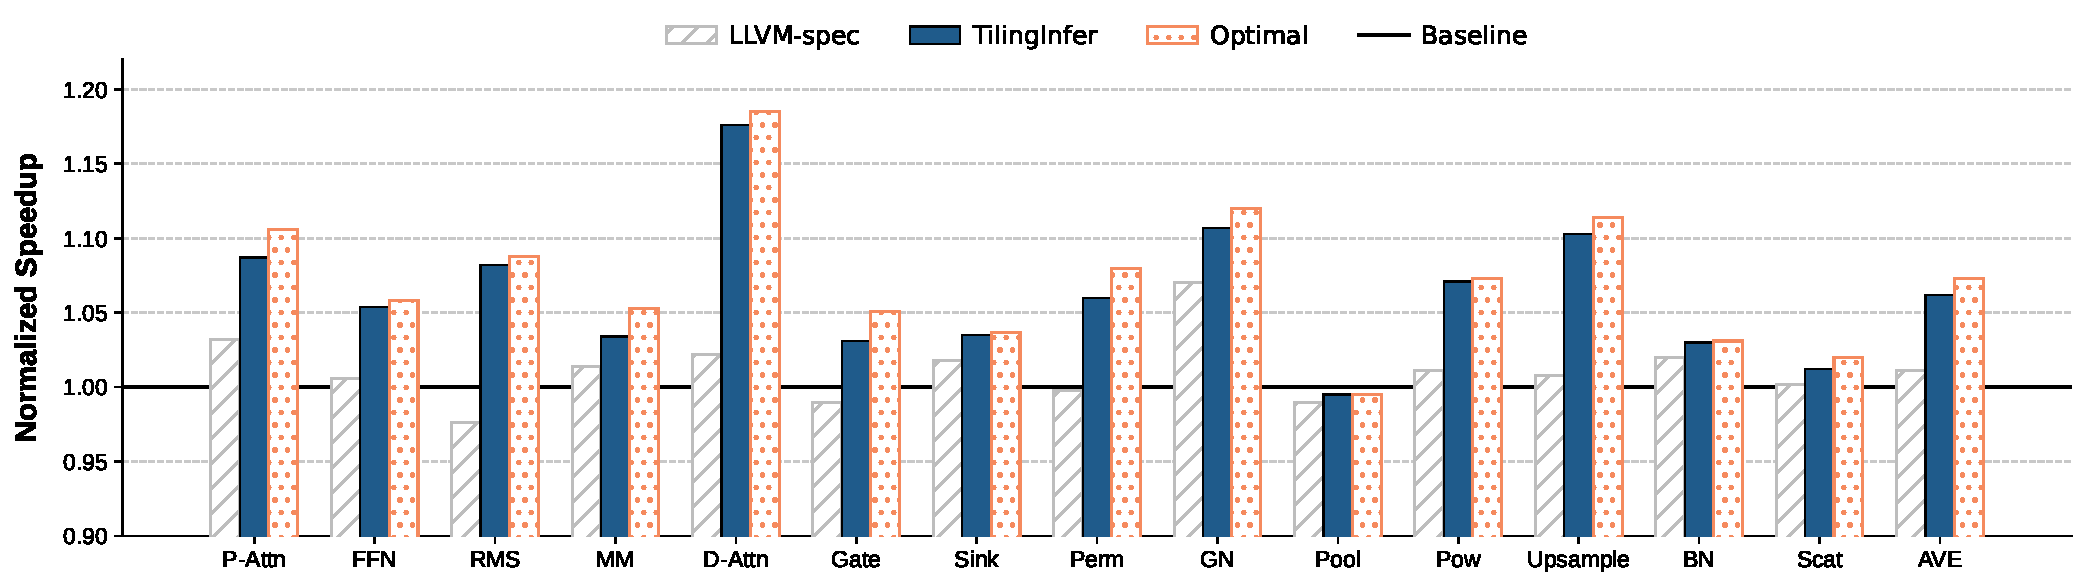
\includegraphics[width=0.95\textwidth]{figures/evaluation/op-speedup/speedup_histogram.pdf}
%DIFDELCMD <     \caption{Overall normalized performance of \textbf{TilingInfer} compared to compiler baselines }
%DIFDELCMD <     \Description{Bar chart showing speedup ratios for different operators comparing TilingInfer, LLVM-spec, and Optimal methods.}
%DIFDELCMD <     \label{fig:eval:op-overall}
%DIFDELCMD <     \vspace{-10pt}
%DIFDELCMD < \end{figure}
%DIFDELCMD < %%%
\DIFdelend \DIFaddbegin \begin{figure}[htbp]
	\centering
	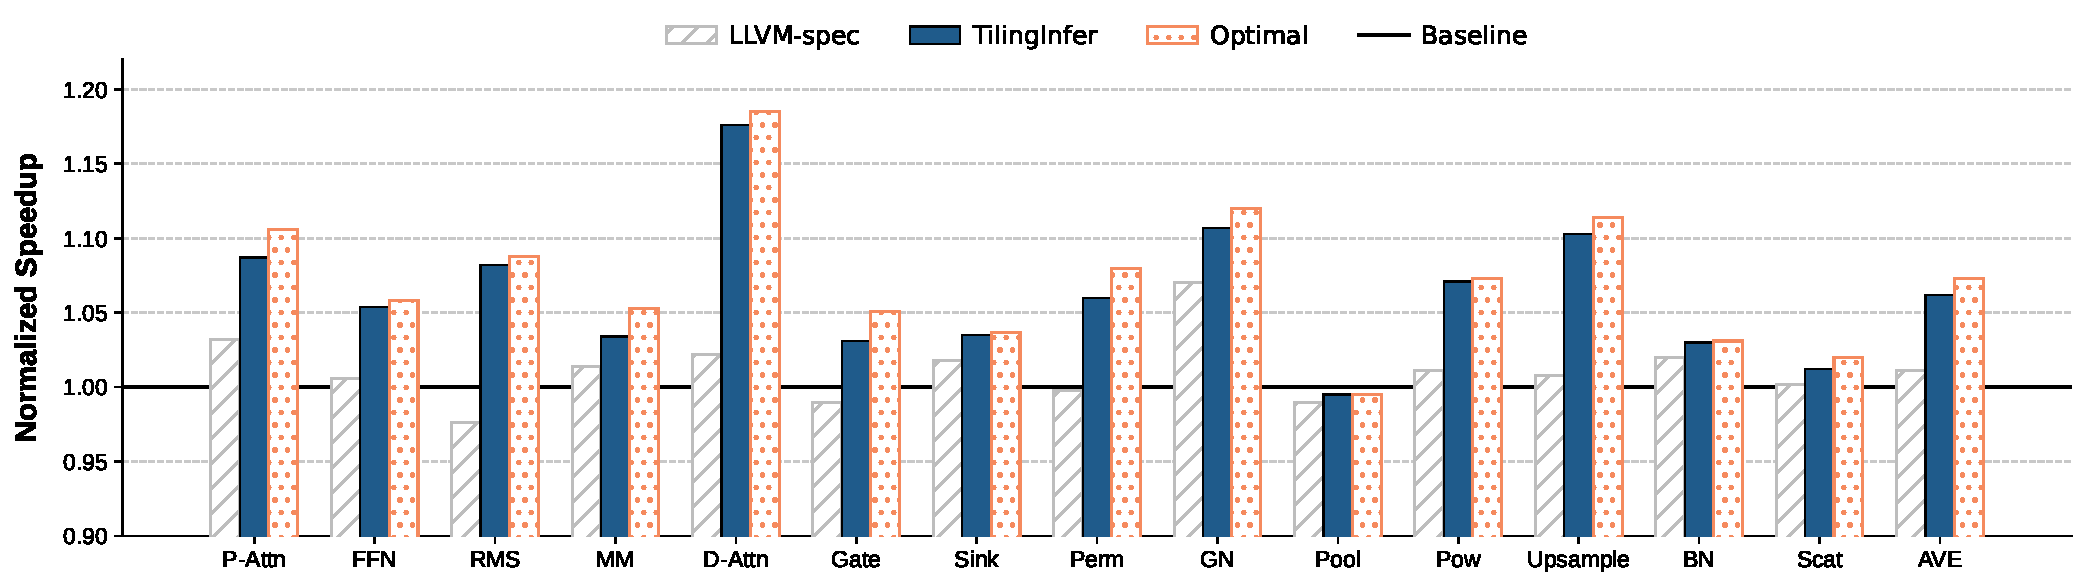
\includegraphics[width=0.75\textwidth]{figures/evaluation/op-speedup/speedup_histogram.pdf}
		\caption{Overall normalized performance of \textbf{TilingInfer} compared to compiler baselines}
		\Description{Bar chart showing speedup ratios for 14 operators comparing LLVM-spec, TilingInfer, and the empirical full-specialization oracle.}
		\label{fig:eval:op-overall}
\end{figure}
\DIFaddend 


Overall, \textbf{TilingInfer} achieves a geometric mean speedup of \textbf{1.06$\times$} across all operators, substantially outperforming the \textbf{LLVM-spec} baseline (1.01$\times$). Crucially, the speedup ratio of \textbf{TilingInfer} is close to that of \textbf{Optimal} (only 1\% smaller on average).
This demonstrates that \textbf{TilingInfer} successfully specializes the majority of \DIFdelbegin \DIFdel{kernel }\DIFdelend \DIFaddbegin \DIFadd{schedule }\DIFaddend parameters, leaving only a few residual parameters that have negligible impact on performance. These results validate that \textbf{TilingInfer} achieves effective automatic kernel specialization for NPU operators.

We observe distinct performance behaviors across operator categories: \textbf{Attention mechanisms} (P-Attn, D-Attn) show the most significant gains, \textbf{1.09$\times$} for P-Attn and \textbf{1.18$\times$} for D-Attn because these \DIFaddbegin \DIFadd{schedule-generic }\DIFaddend kernels have a large number of schedule parameters.
RMS and GN also benefit notably (\textbf{1.08$\times$} and \textbf{1.11$\times$}), as constant specialization eliminates redundant boundary checks and simplifies division operations.

\subsubsection{\DIFaddbegin \DIFadd{Representative }\DIFaddend End-to-End \DIFdelbegin \DIFdel{Model Performance Analysis}\DIFdelend \DIFaddbegin \DIFadd{Inference Scenarios}\DIFaddend}
\DIFdelbegin
%DIFDELCMD < %%%
\DIFdel{The end-to-end model inference performance is depicted in }%DIFDELCMD < \autoref{fig:eval:model-overall}%%%
\DIFdel{, showing normalized speedup for Llama-3.2-3B and Qwen2.5-1.5B across varying sequence lengths and batch sizes (BS=1, 2, 4) during both Prefill and Decode phases. Additionally, }%DIFDELCMD < \autoref{fig:eval:operator-breakdown} %%%

\DIFdel{presents the operator latency breakdown to illustrate the contribution of different operators to the total inference time. }%DIFDELCMD < 

%DIFDELCMD < \begin{figure}
%DIFDELCMD <     \centering
%DIFDELCMD <     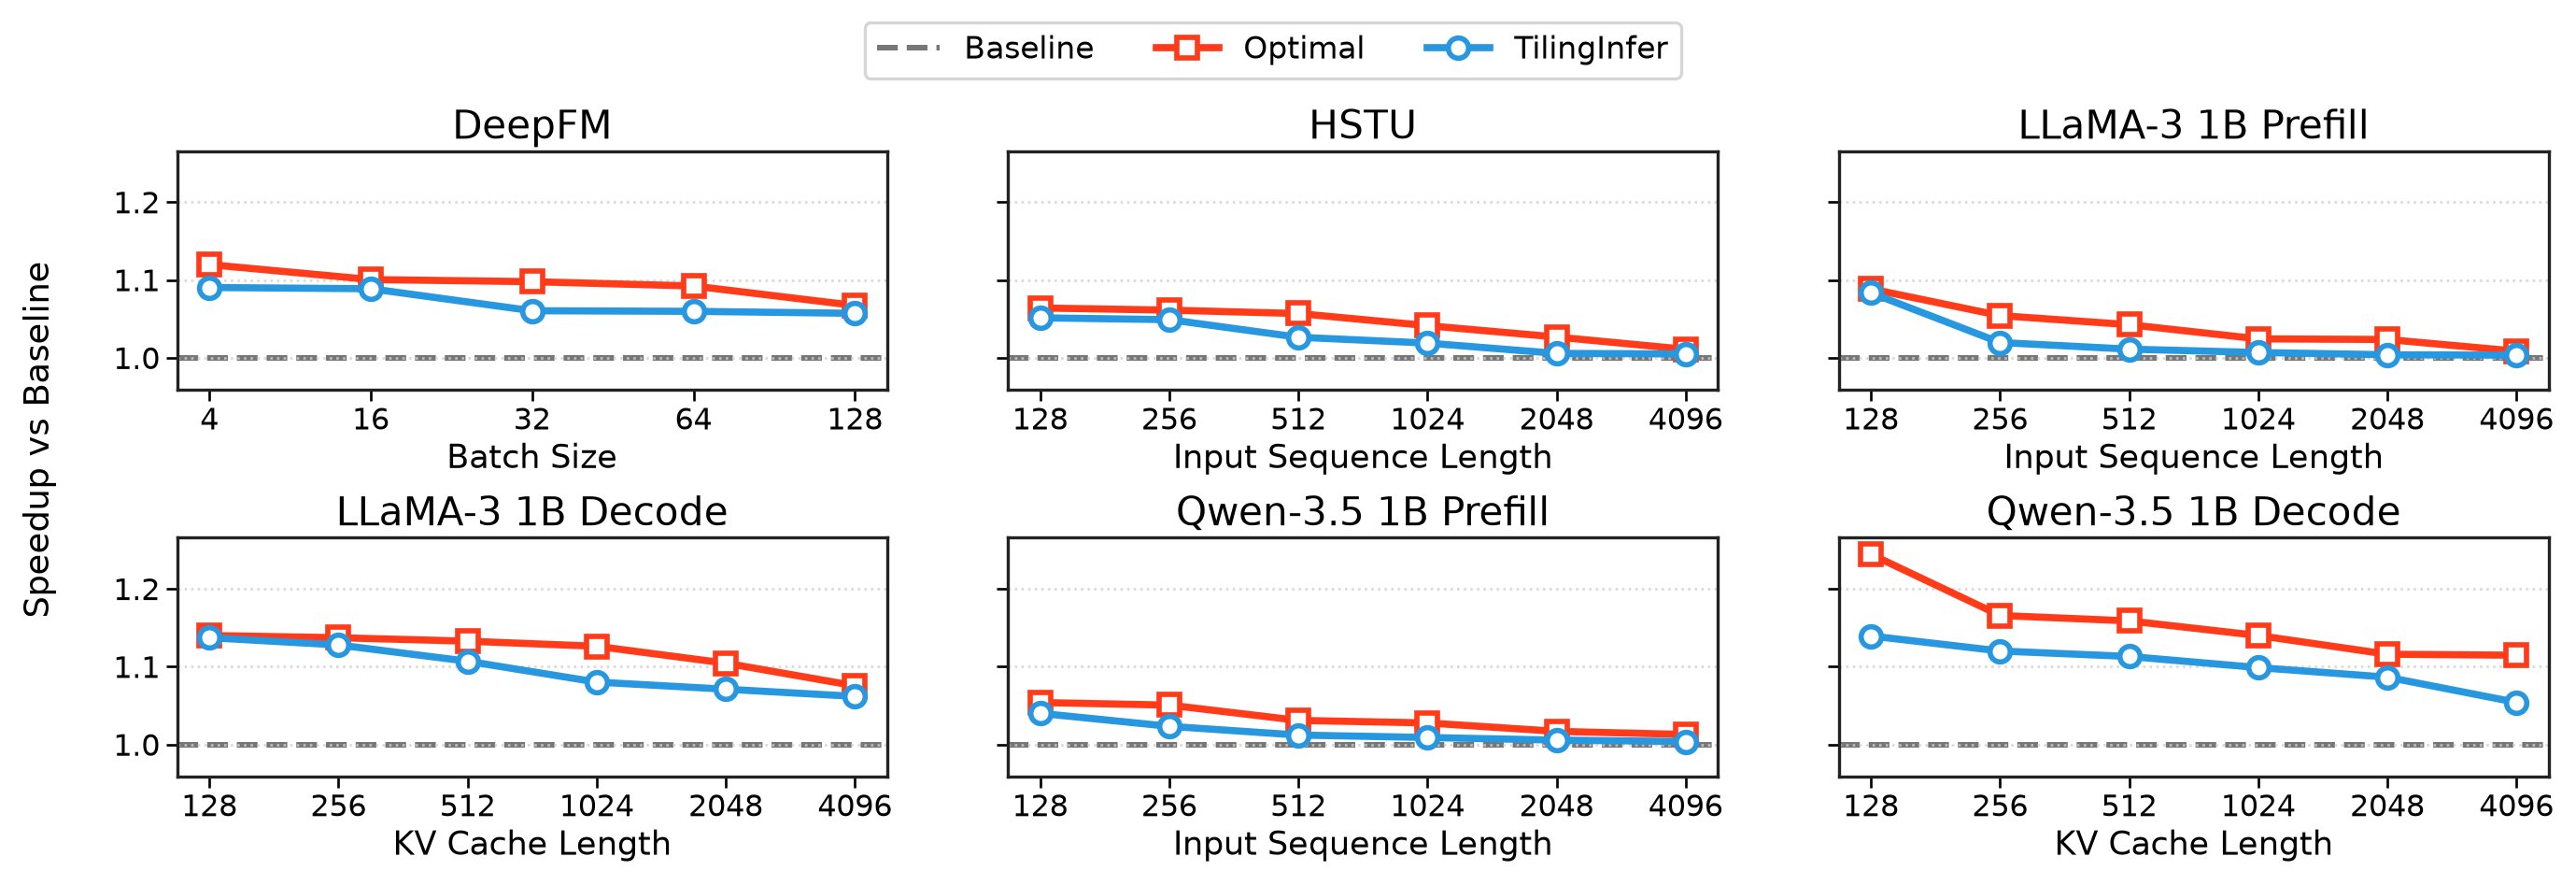
\includegraphics[width=\textwidth]{figures/evaluation/model-speedup/multi_model_speedup.png}
%DIFDELCMD <     \caption{End-to-end speedup of \textbf{TilingInfer} compared to PyTorch baseline based on CANN compiler for Llama-3.2-3B and Qwen2.5-1.5B. For the prefill phase, we measure the time to first token (TTFT); for the decode phase, we measure the inter-token latency (ITL).}
%DIFDELCMD <     \Description{End-to-end speedup of \textbf{TilingInfer} compared to PyTorch baseline based on CANN compiler for Llama-3.2-3B and Qwen2.5-1.5B.}
%DIFDELCMD <     \label{fig:eval:model-overall}
%DIFDELCMD <     \vspace{-10pt}
%DIFDELCMD < \end{figure}
%DIFDELCMD < %%%
\DIFdelend

\DIFadd{The shape configurations of the six representative inference scenarios are summarized in }\autoref{tab:eval:model-configs}\DIFadd{, and their operator calls are classified in }\autoref{tab:eval:model-operator-categories}\DIFadd{. We divide the calls into seven categories. MatMul/GMM, Attention, and Norm invoke CANN kernels from a schedule-generic implementation and together account for approximately 40\%--94\% of model-inference latency. The other four categories use kernels generated by TVM~\mbox{%DIFAUXCMD
\cite{chen2018tvm}}\hspace{0pt}%DIFAUXCMD
, an AI compiler that provides a Python-embedded DSL for describing operator implementations. These kernels have simple schedules, with schedule parameters already specialized during code generation, so TilingInfer provides no further speedup for them.
}\DIFaddend 

\DIFdelbegin %DIFDELCMD < \begin{figure}
%DIFDELCMD <     \centering
%DIFDELCMD <     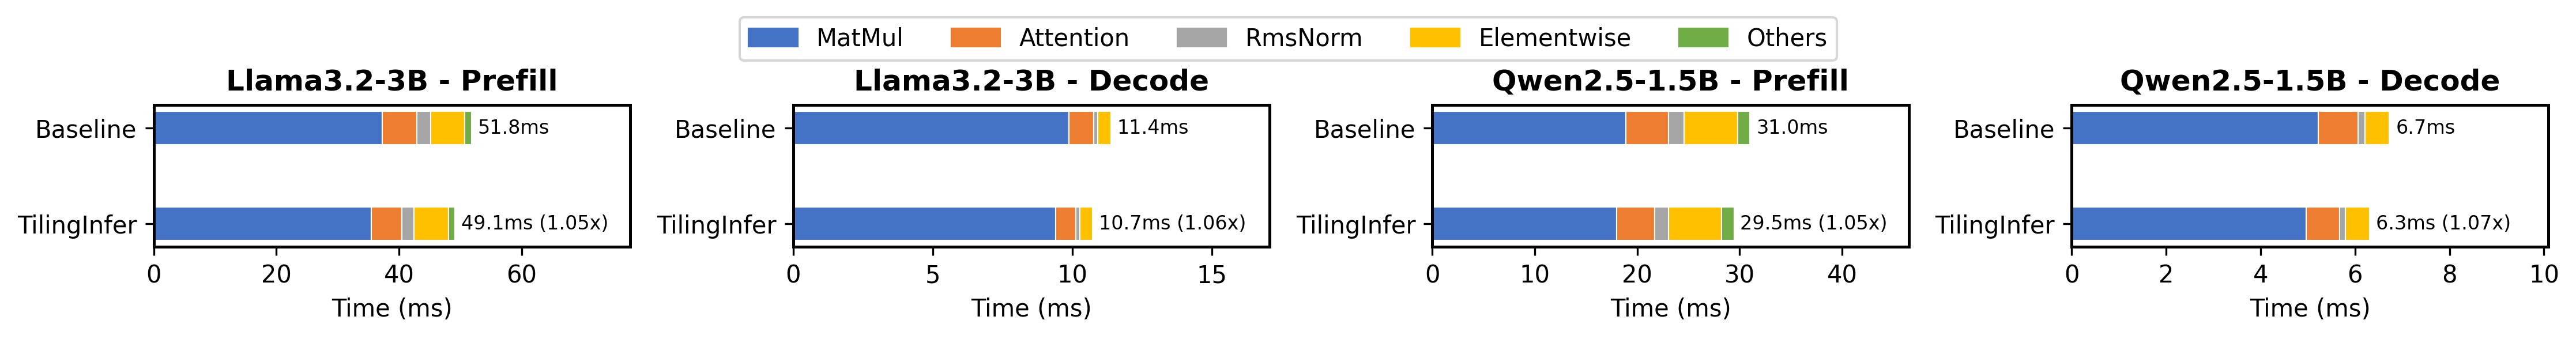
\includegraphics[width=\textwidth]{figures/evaluation/model-speedup/operator_breakdown.png}
%DIFDELCMD <     \caption{Operator latency breakdown for Llama-3.2-3B and Qwen2.5-1.5B during inference, showing the proportion of execution time attributed to each operator type. The statistics are computed as the average total execution time of operator kernel functions across batch sizes of 1, 2, and 4, with input/output sequence lengths ranging from 32 to 2048. Since NPU idle time is excluded from this measurement, the reported speedup is higher than that shown in \autoref{fig:eval:model-overall}. Note that FusedFFN is absent because the PyTorch deployment does not utilize this fused operator.}
%DIFDELCMD <     \Description{Operator latency breakdown for Llama-3.2-3B and Qwen2.5-1.5B during inference.}
%DIFDELCMD <     \label{fig:eval:operator-breakdown}
%DIFDELCMD <     \vspace{-10pt}
%DIFDELCMD < \end{figure}
%DIFDELCMD < %%%
\DIFdelend \DIFaddbegin \begin{figure}[t]
	\centering
	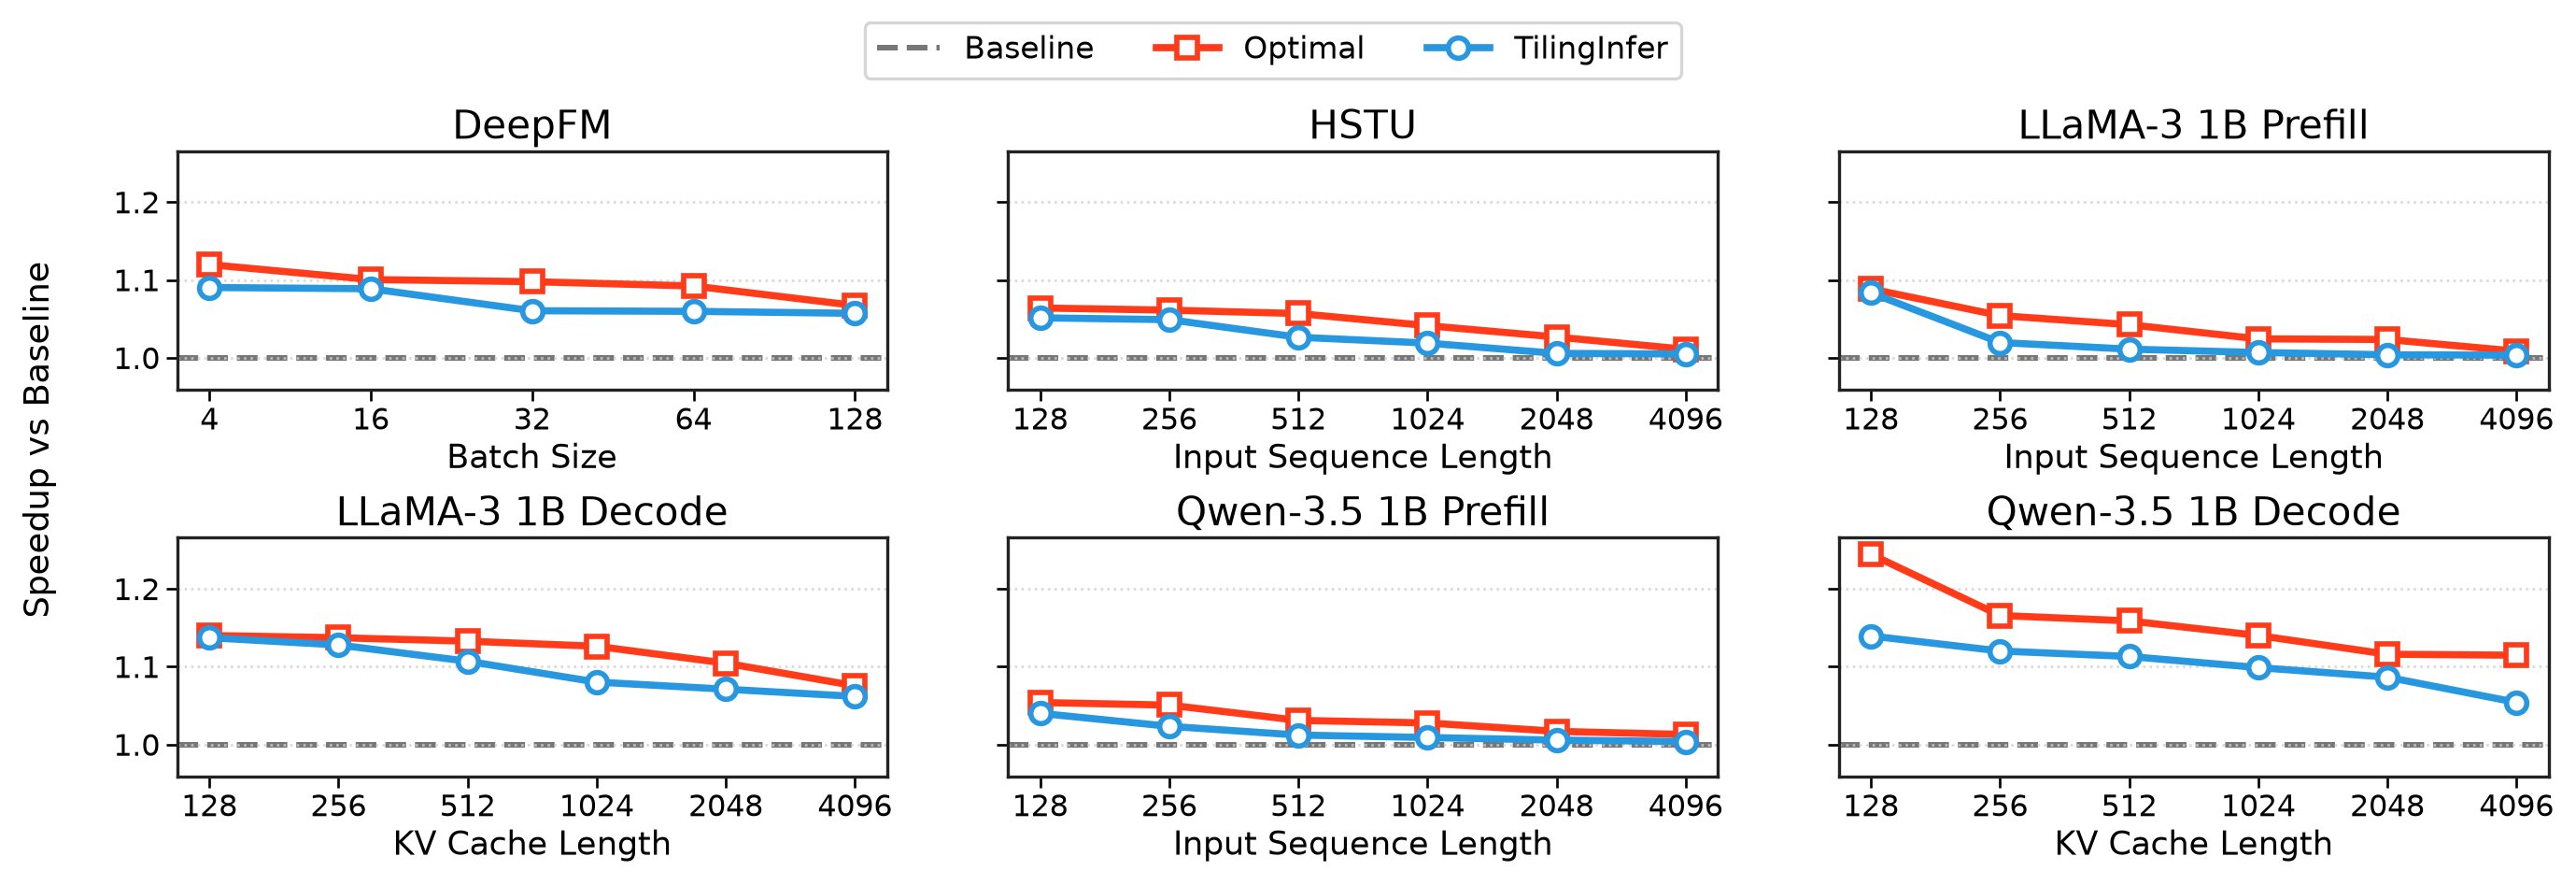
\includegraphics[width=0.78\textwidth]{figures/evaluation/model-speedup/multi_model_speedup.png}
		\caption{End-to-end speedup versus runtime shape for six representative ML inference scenarios.}
		\Description{End-to-end speedup trends for DeepFM, HSTU, LLaMA prefill and decode, and Qwen prefill and decode.}
		\label{fig:eval:model-overall}
\end{figure}
\DIFaddend 

\DIFdelbegin \DIFdel{As shown in }%DIFDELCMD < \autoref{fig:eval:model-overall}%%%
\DIFdel{, }\textbf{%DIFDELCMD < TilingInfer%%%
} %DIFAUXCMD
\DIFdel{achieves an average speedup of }\textbf{\DIFdel{3\%}} %DIFAUXCMD
\DIFdel{across various shape configurations for both Prefill and Decode phases.
The speedup is more pronounced for shorter sequences, but }\DIFdelend \DIFaddbegin \autoref{fig:eval:model-overall} \DIFadd{shows that }TilingInfer\DIFadd{'s end-to-end speedup generally }\DIFaddend decreases as the \DIFdelbegin \DIFdel{input length and the number of generated tokens increase.
This trend is consistent across both phases. }\DIFdelend \DIFaddbegin \DIFadd{runtime shape grows because tensor computation occupies an increasing fraction of execution time. DeepFM and the two decode scenarios obtain the larger gains, averaging approximately 1.10$\times$, whereas HSTU and the two prefill scenarios average approximately 1.03$\times$. Relative to Optimal's per-shape full specialization, }TilingInfer \DIFadd{achieves comparable geometric-mean speedups---1.05$\times$ versus 1.08$\times$ across all six scenarios and 1.10$\times$ versus 1.14$\times$ across the two decode scenarios; although faster, Optimal recompiles the entire operator for every shape, taking tens of minutes each and thus being impractical in production.
}\DIFaddend 

\DIFdelbegin \DIFdel{We make two key observations. First, }\textbf{\DIFdel{Speedup Variation with Sequence Length}}%DIFAUXCMD
\DIFdel{, the end-to-end speedup is more significant for small sequences where scalar overhead is proportionally larger ; as sequence length increases, computational workload dominates, decreasing the benefit. Second, }\textbf{\DIFdel{Dominance of MatMul}}%DIFAUXCMD
\DIFdel{, MatMul accounts for the majority of inference time; although }\textbf{%DIFDELCMD < TilingInfer%%%
} %DIFAUXCMD
\DIFdel{achieves significant speedups for FlashAttention and normalization, these contribute less to overall latency, resulting in modest end-to-end improvement}\DIFdelend \DIFaddbegin \begin{table}[H]
	\caption{Operator categories, implementation sources, and TilingInfer outcomes for the six representative models.}
	\Description{The seven model-operator categories, their simplified operator names, whether they use the CANN library or AI-compiler-generated kernels, and whether TilingInfer specialization provides a benefit.}
	\label{tab:eval:model-operator-categories}
	\centering
	\scriptsize
	\setlength{\tabcolsep}{3pt}
	\renewcommand{\arraystretch}{0.88}
	\begin{tabularx}{\columnwidth}{@{}l>{\raggedright\arraybackslash}Xl@{}}
		\toprule
		\textbf{Category} & \textbf{Operators} & \textbf{Implementation source / outcome} \\
		\midrule
		MatMul/GMM &
		Matrix Multiplication (MM), Batched Matrix Multiplication (BMM), Grouped Matrix Multiplication (GMM) &
		\multirow{3}{*}{\shortstack[l]{CANN operator library;\\TilingInfer specialization benefits}} \\
		Attention & P-Attn, D-Attn & \\
		Norm & RMSNorm, LayerNorm, GroupNorm & \\
		\midrule
		Embedding/Gather & Embedding, Gather &
		\multirow{4}{*}{\shortstack[l]{AI-compiler-generated kernels (TVM Python DSL);\\no TilingInfer specialization benefit}} \\
		Activation/Softmax & ReLU, SiLU/Swish, GELU, Sigmoid, Tanh, Softmax, Reduce/Mean & \\
		Pointwise Arithmetic & Add, Sub, Mul, Div, Pow, Rsqrt, Maximum/Minimum, Zero & \\
		Layout \& Data Movement & Concat, Slice, Transpose, Cast, Copy/TensorMove, Reshape/AsStrided & \\
		\bottomrule
	\end{tabularx}
	\vspace{-6pt}
\end{table}

\begin{figure}[t]
	\centering
	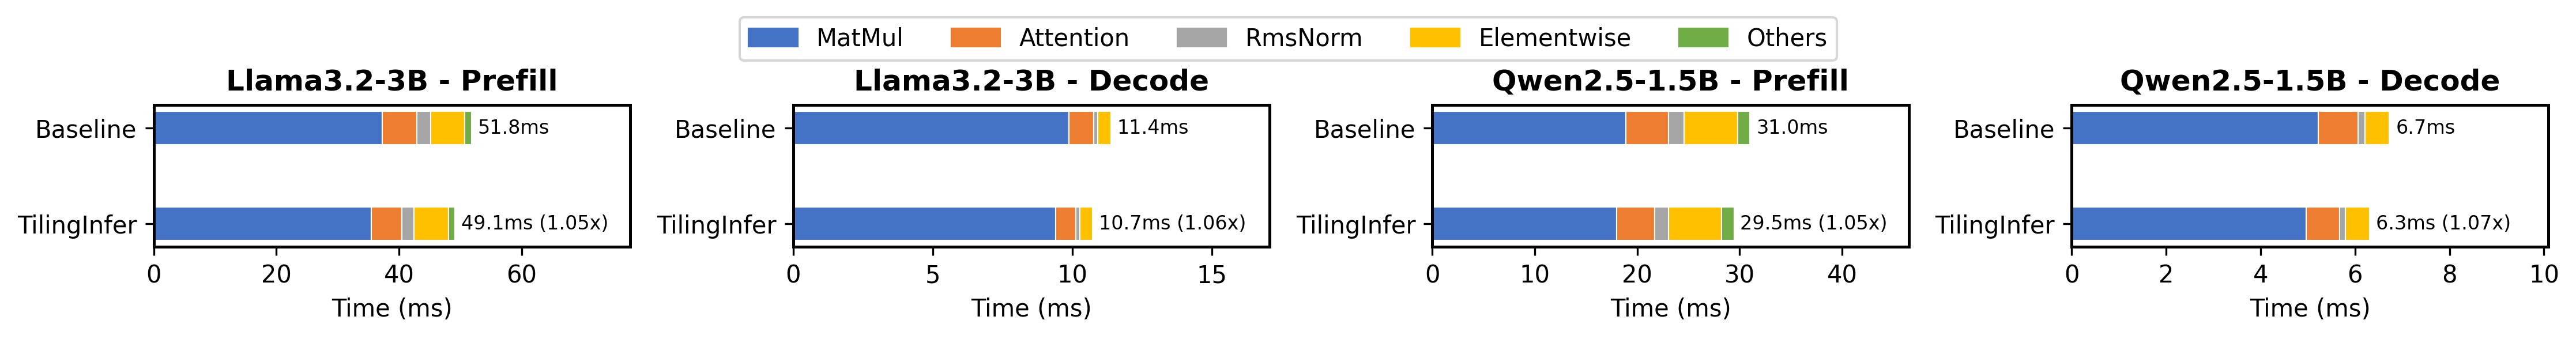
\includegraphics[width=0.78\textwidth]{figures/evaluation/model-speedup/operator_breakdown.png}
		\caption{Device-kernel latency analysis for six inference scenarios at representative shapes.}
		\Description{Baseline device-kernel latency composition and TilingInfer-over-Baseline operator speedups across seven categories and six representative inference scenarios.}
		\label{fig:eval:operator-breakdown}
\end{figure}

\autoref{fig:eval:operator-breakdown} \DIFadd{attributes the model-level gains primarily to Attention and MatMul/GMM. In particular, the MatMul calls in DeepFM and decode phase of LLMs have relatively small computation sizes, so specialization removes a larger fraction of their tiling and control overhead and produces higher operator speedups. Attention supplies the other major source of improvement, especially in the decode phase. By contrast, the four AI-compiler-generated categories remain at 1.00$\times$, confirming that }TilingInfer\DIFadd{'s benefits are limited to expert-written operators}\DIFaddend .

\subsubsection{Comparison between \textbf{TilingInfer} and specialization based on Standard LLVM}

\autoref{tab:compilation_detail} shows the trade-off between compilation overhead and optimization effects.
\textbf{LLVM-spec} incurs minimal overhead (less than 0.60s) due to its \DIFdelbegin \DIFdel{inprecise }\DIFdelend \DIFaddbegin \DIFadd{imprecise }\DIFaddend analysis.
In contrast, \textbf{TilingInfer} exhibits \DIFaddbegin \DIFadd{a }\DIFaddend moderate increase (0.24s to 2.70s) due to field-sensitive analysis.
Given that this compilation is a one-off cost during deployment, we consider this overhead acceptable, as it enables the backend compiler to generate considerably more efficient binaries (1.06$\times$ speedup).
Moreover, \textbf{TilingInfer} avoids employing path-sensitive analysis through early-exit path identification, keeping compilation overhead acceptable.

%DIF <  TODO:
%DIF <  Comparison of the number of inferred parameters
\DIFaddbegin \begin{table}[H]
    \centering
    \caption{Detailed comparison of compilation overhead and parameter specialization.
    \textbf{Total Params} indicates the number of schedule parameters defined in the operator program.
    \textbf{Time} is total compilation time in seconds. \textbf{Diff} is the time increment relative to Baseline.
    \textbf{Derived \#} is the count of invariant schedule parameters inferred by the compiler.}
    \label{tab:compilation_detail}
    \resizebox{\textwidth}{!}{%
    \begin{tabular}{@{}llcccccccccccccc@{}}
    \toprule
    \multicolumn{2}{c}{\textbf{Operator}} & \textbf{P-Attn} & \textbf{D-Attn} & \textbf{MM} & \textbf{FFN} & \textbf{RMS} & \textbf{Gate} & \textbf{Sink} & \textbf{Perm} & \textbf{GN} & \textbf{Pool} & \textbf{Pow} & \textbf{Upsample} & \textbf{BN} & \textbf{Scat} \\
    \midrule
    \multicolumn{2}{c}{\textbf{Total Params}} & \textbf{264} & \textbf{389} & \textbf{72} & \textbf{123} & \textbf{15} & \textbf{60} & \textbf{20} & \textbf{42} & \textbf{23} & \textbf{17} & \textbf{10} & \textbf{143} & \textbf{22} & \textbf{20} \\
    \midrule
    \textbf{Baseline} & Time (s) & 24.50 & 19.80 & 42.10 & 4.52 & 3.12 & 1.85 & 5.10 & 1.24 & 6.15 & 1.35 & 0.82 & 2.95 & 3.30 & 1.15 \\
    \midrule
    \multirow{3}{*}{\textbf{LLVM-Spec}} 
     & Time (s) & 25.10 & 20.15 & 42.45 & 4.65 & 3.20 & 1.92 & 5.30 & 1.30 & 6.40 & 1.40 & 0.88 & 3.10 & 3.35 & 1.20 \\
     & \textit{Diff} & \scriptsize{(+0.60)} & \scriptsize{(+0.35)} & \scriptsize{(+0.35)} & \scriptsize{(+0.13)} & \scriptsize{(+0.08)} & \scriptsize{(+0.07)} & \scriptsize{(+0.20)} & \scriptsize{(+0.06)} & \scriptsize{(+0.25)} & \scriptsize{(+0.05)} & \scriptsize{(+0.06)} & \scriptsize{(+0.15)} & \scriptsize{(+0.05)} & \scriptsize{(+0.05)} \\
     & Derived \# & 4 & 3 & 3 & 2 & 1 & 2 & 0 & 0 & 1 & 0 & 0 & 3 & 2 & 1 \\
    \midrule
    \multirow{3}{*}{\textbf{TilingInfer}} 
     & Time (s) & 27.20 & 21.05 & 42.95 & 5.42 & 3.58 & 2.25 & 6.95 & 1.65 & 7.25 & 1.62 & 1.15 & 3.55 & 3.54 & 1.52 \\
     & \textit{Diff} & \scriptsize{(+2.70)} & \scriptsize{(+1.25)} & \scriptsize{(+0.85)} & \scriptsize{(+0.90)} & \scriptsize{(+0.46)} & \scriptsize{(+0.40)} & \scriptsize{(+1.85)} & \scriptsize{(+0.41)} & \scriptsize{(+1.10)} & \scriptsize{(+0.27)} & \scriptsize{(+0.33)} & \scriptsize{(+0.60)} & \scriptsize{(+0.24)} & \scriptsize{(+0.37)} \\
     & Derived \# & 242 & 352 & 60 & 110 & 11 & 30 & 13 & 28 & 17 & 15 & 5 & 82 & 15 & 14 \\
    \bottomrule
    \end{tabular}%
    }
\end{table}
\DIFaddend 


\DIFdelbegin %DIFDELCMD < \begin{table}[htbp]
%DIFDELCMD <     \centering
%DIFDELCMD <     \caption{Detailed comparison of compilation overhead and parameter specialization. 
%DIFDELCMD <     \textbf{Total Params} indicates the number of parameter fields defined in the operator program.
%DIFDELCMD <     \textbf{Time} is total compilation time in seconds. \textbf{Diff} is the time increment relative to Baseline.
%DIFDELCMD <     \textbf{Derived \#} is the count of invariant parameter fields inferred by the compiler.}
%DIFDELCMD <     \label{tab:compilation_detail}
%DIFDELCMD <     \vspace{-5pt}
%DIFDELCMD <     \resizebox{\textwidth}{!}{%
%DIFDELCMD <     \begin{tabular}{@{}llcccccccccccccc@{}}
%DIFDELCMD <     \toprule
%DIFDELCMD <     \multicolumn{2}{c}{\textbf{Operator}} & \textbf{P-Attn} & \textbf{D-Attn} & \textbf{MM} & \textbf{FFN} & \textbf{RMS} & \textbf{Gate} & \textbf{Sink} & \textbf{Perm} & \textbf{GN} & \textbf{Pool} & \textbf{Pow} & \textbf{Upsample} & \textbf{BN} & \textbf{Scat} \\
%DIFDELCMD <     \midrule
%DIFDELCMD <     \multicolumn{2}{c}{\textbf{Total Params}} & \textbf{264} & \textbf{389} & \textbf{72} & \textbf{123} & \textbf{15} & \textbf{60} & \textbf{20} & \textbf{42} & \textbf{23} & \textbf{17} & \textbf{10} & \textbf{143} & \textbf{22} & \textbf{20} \\
%DIFDELCMD <     \midrule
%DIFDELCMD <     \textbf{Baseline} & Time (s) & 24.50 & 19.80 & 42.10 & 4.52 & 3.12 & 1.85 & 5.10 & 1.24 & 6.15 & 1.35 & 0.82 & 2.95 & 3.30 & 1.15 \\
%DIFDELCMD <     \midrule
%DIFDELCMD <     \multirow{3}{*}{\textbf{LLVM-Spec}} 
%DIFDELCMD <      & Time (s) & 25.10 & 20.15 & 42.45 & 4.65 & 3.20 & 1.92 & 5.30 & 1.30 & 6.40 & 1.40 & 0.88 & 3.10 & 3.35 & 1.20 \\
%DIFDELCMD <      & \textit{Diff} & \scriptsize{(+0.60)} & \scriptsize{(+0.35)} & \scriptsize{(+0.35)} & \scriptsize{(+0.13)} & \scriptsize{(+0.08)} & \scriptsize{(+0.07)} & \scriptsize{(+0.20)} & \scriptsize{(+0.06)} & \scriptsize{(+0.25)} & \scriptsize{(+0.05)} & \scriptsize{(+0.06)} & \scriptsize{(+0.15)} & \scriptsize{(+0.05)} & \scriptsize{(+0.05)} \\
%DIFDELCMD <      & Derived \# & 4 & 3 & 3 & 2 & 1 & 2 & 0 & 0 & 1 & 0 & 0 & 3 & 2 & 1 \\
%DIFDELCMD <     \midrule
%DIFDELCMD <     \multirow{3}{*}{\textbf{TilingInfer}} 
%DIFDELCMD <      & Time (s) & 27.20 & 21.05 & 42.95 & 5.42 & 3.58 & 2.25 & 6.95 & 1.65 & 7.25 & 1.62 & 1.15 & 3.55 & 3.54 & 1.52 \\
%DIFDELCMD <      & \textit{Diff} & \scriptsize{(+2.70)} & \scriptsize{(+1.25)} & \scriptsize{(+0.85)} & \scriptsize{(+0.90)} & \scriptsize{(+0.46)} & \scriptsize{(+0.40)} & \scriptsize{(+1.85)} & \scriptsize{(+0.41)} & \scriptsize{(+1.10)} & \scriptsize{(+0.27)} & \scriptsize{(+0.33)} & \scriptsize{(+0.60)} & \scriptsize{(+0.24)} & \scriptsize{(+0.37)} \\
%DIFDELCMD <      & Derived \# & 242 & 352 & 60 & 110 & 11 & 30 & 13 & 28 & 17 & 15 & 5 & 82 & 15 & 14 \\
%DIFDELCMD <     \bottomrule
%DIFDELCMD <     \end{tabular}%
%DIFDELCMD <     }
%DIFDELCMD <     \vspace{-15pt}
%DIFDELCMD < \end{table}
%DIFDELCMD < %%%
\clearpage
\subsection{Device-Level Attribution}
\label{sec:eval:analysis}

\input{tables/benefits-all}

\begin{figure}[H]
	\centering
	\begin{subfigure}[t]{0.40\textwidth}
		\centering
		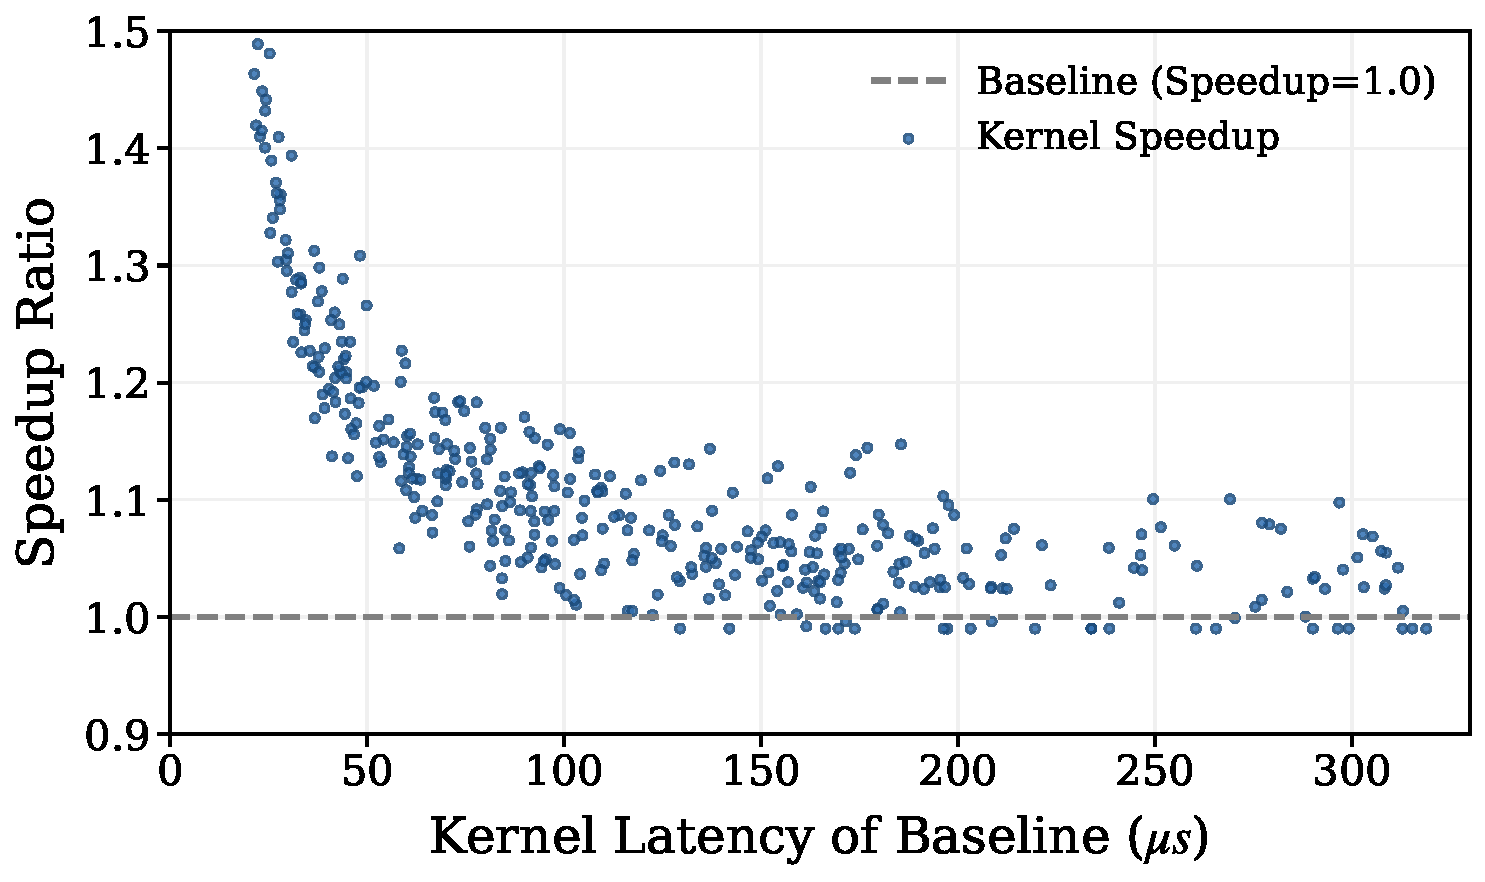
\includegraphics[width=\linewidth]{figures/evaluation/op-speedup/d_attn_execution_speedup.pdf}
		\caption{D-Attn}
	\end{subfigure}
	\hfill
	\begin{subfigure}[t]{0.40\textwidth}
		\centering
		\includegraphics[width=\linewidth]{figures/evaluation/op-speedup/mm_execution_speedup.pdf}
		\caption{MM}
	\end{subfigure}
	\caption{Kernel speedup versus Baseline device-kernel latency for D-Attn and MM. Blue points report the speedup of TilingInfer relative to Baseline.}
	\Description{Two scatter plots showing TilingInfer kernel speedup versus Baseline device-kernel latency for D-Attn and MM.}
	\label{fig:eval:op-scaling}
\end{figure}

\FloatBarrier

{\color{red}%
\DIFdel{%
To gain deeper insight into the sources of performance gains demonstrated in Section~}\ref{sec:eval:result}\DIFdel{, we analyze low-level hardware performance metrics collected during operator execution. }\autoref{tab:performance_metrics}\DIFdel{ details the Speedup alongside key architectural metrics: Instruction Cache (I-Cache) Miss Rate, Scalar Instruction Ratio, Memory Access (Read and Write) Ratios, and the final compiled Binary Size. The Scalar Ratio, Memory Read Ratio, and Memory Write Ratio quantify the proportion of execution cycles of corresponding hardware units (scalar units, memory read/write units) relative to the total kernel execution cycles. Comparing TilingInfer (T) against the Baseline (B) and LLVM-spec (L), we attribute the improvements to two primary factors: reduced instruction fetch overhead and simplified runtime calculation.
}
\par}

{\color{red}%
\DIFdel{%
Reduction in Binary Size and I-Cache Misses. By propagating runtime invariants, TilingInfer enables the backend compiler to aggressively perform Dead Code Elimination (DCE) and simplify control flow graphs. This leads to significant binary size reductions: 34.0\% for Upsample, 22.7\% for D-Attn, 20.2\% for FFN, and 14.8\% for P-Attn. Consequently, the I-Cache Miss rate drops substantially: Upsample (9.83\% $\rightarrow$ 0.12\%), D-Attn (4.45\% $\rightarrow$ 0.18\%), FFN (3.89\% $\rightarrow$ 0.15\%), and P-Attn (16.40\% $\rightarrow$ 11.39\%). These improvements in instruction fetch efficiency contribute to the observed speedups.
}
\par}

{\color{red}%
\DIFdel{%
Optimization of Computational Intensity and Memory Schedule. TilingInfer substantially reduces the Scalar Ratio for operators like RMS (97.9\% $\rightarrow$ 88.6\%) and Pow (59.5\% $\rightarrow$ 53.1\%), confirming that resolving loop bounds and offsets at compile time effectively converts runtime scalar calculations into immediate operands. The Memory Read Ratio also improves, dropping from 25.0\% to 16.4\% for Gate and from 25.0\% to 18.8\% for GN. This reduction is primarily due to the decreased number of parameters read from device memory, as well as the compiler's ability to merge multiple memory accesses when loop iteration counts are determined at compile time. Furthermore, optimizations such as loop unrolling can facilitate instruction scheduling and effectively hide memory access latency. These factors collectively contribute to the speedups observed in operators such as D-Attn, Pow, and RMS.
}
\par}

{\color{red}%
\DIFdel{%
Insensitive Operators. Some operators, such as Pool and Scat, show negligible speedups (1.00$\times$--1.01$\times$). For Pool, the Baseline binary size is already minimal (13.35KB) with 0.08\% I-Cache miss rate, leaving no room for control flow simplification. For Scat, the overhead of scalar instructions and instruction fetching is minimal compared to memory-bound operations. Optimizations in the instruction stream do not translate into visible latency reductions when the bottleneck lies in memory or arithmetic units.
}
\par}

{\color{red}%
\DIFdel{%
Impact of Workload Scale. The original varying-KV-length and latency-distribution results show that speedup decreases towards 1.0 as workload increases. This implies that performance benefits from kernel specialization are relatively fixed in absolute time. Consequently, this fixed reduction yields significant speedup ratios for small-scale kernels but becomes negligible for heavy workloads dominated by computation and memory access.
}
\par}

{\color{blue}%
\autoref{tab:performance_metrics} and \autoref{fig:eval:op-scaling} show that TilingInfer does not produce uniform device-level gains; benefiting kernels fall into two mechanism-driven classes, whereas a third class is largely insensitive. For Upsample, D-Attn, FFN, and P-Attn, gains mainly arise because invariant propagation exposes constant branches and loop structure, enabling dead-code elimination and control-flow simplification; the resulting smaller instruction footprint reduces instruction-fetch and I-Cache pressure. A second class, including RMS, Pow, Gate, and GN, benefits primarily from simplified runtime calculation and memory scheduling. Resolving loop bounds, offsets, and schedule parameters removes scalar loads and address or control computations, exposes immediate operands, and enables access merging, loop unrolling, and more effective instruction scheduling. In contrast, Pool and Scat are largely insensitive: Pool is already compact with little instruction-fetch overhead, whereas Scat is dominated by memory work, so instruction-stream simplification does not shorten the critical path. Across all three classes, specialization mainly removes a roughly fixed amount of control and scheduling overhead. Its relative effect is therefore strongest for short-running kernels and diminishes as tensor computation or memory traffic dominates. The key determinant is not whether a parameter is static, but whether resolving it eliminates work on the kernel's performance-critical path.
\par}

\begin{comment}
\DIFdelend \DIFaddbegin \subsection{\DIFadd{Device-Level Attribution}}
\label{sec:eval:analysis}
\DIFaddend 

\DIFdelbegin \subsection{\DIFdel{Detailed Analysis on Benefits of }\textbf{%DIFDELCMD < TilingInfer%%%
}%DIFAUXCMD
}
%DIFAUXCMD
\addtocounter{subsection}{-1}%DIFAUXCMD
\DIFdelend \DIFaddbegin \begin{table}[htbp]
\centering
\caption{Performance Comparison: Speedup and detailed hardware metrics across \textbf{Baseline} (B), \textbf{LLVM-spec} (L), and \textbf{TilingInfer} (T).
Best values are bolded.
Reflecting our goal to maximize time spent on tensor computation units (Cube and Vector), $\downarrow$ denotes lower is better for metrics irrelative to tensor computations. $\uparrow$ denotes higher is better for speedup ratio.}
\label{tab:performance_metrics}
\vspace{2pt}
\renewcommand{\arraystretch}{0.86}
\resizebox{\textwidth}{!}{%
\begin{tabular}{lcccccccccccccccccc}
\toprule
\multirow{2}{*}{\textbf{Op}} & \multicolumn{3}{c}{\textbf{Speedup} ($\uparrow$)} & \multicolumn{3}{c}{\textbf{I-Cache Miss (\%)} ($\downarrow$)} & \multicolumn{3}{c}{\textbf{Scalar Ratio (\%)} ($\downarrow$)} & \multicolumn{3}{c}{\textbf{Mem Read Ratio (\%)} ($\downarrow$)} & \multicolumn{3}{c}{\textbf{Mem Write Ratio (\%)} ($\downarrow$)} & \multicolumn{3}{c}{\textbf{Binary Size(KB)} ($\downarrow$)} \\
\cmidrule(lr){2-4} \cmidrule(lr){5-7} \cmidrule(lr){8-10} \cmidrule(lr){11-13} \cmidrule(lr){14-16} \cmidrule(lr){17-19}
 & \textbf{B} & \textbf{L} & \textbf{T} & \textbf{B} & \textbf{L} & \textbf{T} & \textbf{B} & \textbf{L} & \textbf{T} & \textbf{B} & \textbf{L} & \textbf{T} & \textbf{B} & \textbf{L} & \textbf{T} & \textbf{B} & \textbf{L} & \textbf{T} \\
\midrule
P-Attn & 1.00 & 1.03 & \textbf{1.08} & 16.40 & 16.30 & \textbf{11.39} & 91.23 & \textbf{90.29} & 90.33 & \textbf{8.26} & 8.30 & 8.95 & 3.94 & \textbf{3.81} & 4.11 & 363.81 & 360.76 & \textbf{310.12} \\
FFN & 1.00 & 1.01 & \textbf{1.05} & 3.89 & 4.12 & \textbf{0.00} & 84.72 & 84.52 & \textbf{83.60} & 6.42 & 7.24 & \textbf{5.49} & \textbf{0.10} & 0.11 & 0.11 & 68.79 & 68.89 & \textbf{54.91} \\
RMS & 1.00 & 0.98 & \textbf{1.08} & \textbf{3.00} & 3.01 & 3.36 & 97.89 & 97.82 & \textbf{88.57} & 6.83 & 7.27 & \textbf{6.72} & \textbf{2.90} & 3.02 & 3.13 & 36.32 & 36.32 & \textbf{33.23} \\
MM & 1.00 & 1.01 & \textbf{1.03} & \textbf{3.12} & 3.42 & 3.41 & 84.70 & 84.74 & \textbf{84.68} & \textbf{42.66} & 47.10 & 45.95 & 0.00 & 0.00 & 0.00 & 101.38 & 101.26 & \textbf{100.84} \\
D-Attn & 1.00 & 1.02 & \textbf{1.17} & 4.45 & 5.51 & \textbf{0.00} & 77.98 & 77.08 & \textbf{74.43} & 6.42 & 6.44 & \textbf{4.91} & 2.46 & \textbf{1.60} & 1.79 & 58.30 & 58.59 & \textbf{45.05} \\
Gate & 1.00 & 0.99 & \textbf{1.03} & 0.00 & 0.00 & 0.00 & \textbf{96.98} & \textbf{96.98} & 96.99 & 25.00 & 24.82 & \textbf{16.43} & 1.17 & \textbf{1.05} & 1.36 & 17.10 & \textbf{17.09} & \textbf{17.09} \\
Sink & 1.00 & 1.02 & \textbf{1.03} & 0.00 & 0.00 & 0.00 & 52.46 & 52.96 & \textbf{50.34} & 4.41 & 4.68 & \textbf{4.34} & 18.60 & 18.14 & \textbf{17.88} & 47.54 & 47.56 & \textbf{47.11} \\ 
Perm & 1.00 & 1.00 & \textbf{1.08} & 0.00 & 0.00 & 0.00 & \textbf{92.34} & 92.58 & 92.62 & 10.55 & \textbf{9.31} & 10.52 & 5.84 & 6.25 & \textbf{5.69} & 24.02 & 24.14 & \textbf{14.40} \\
GN & 1.00 & 1.07 & \textbf{1.11} & 0.80 & 1.20 & \textbf{0.00} & 99.10 & 98.94 & \textbf{98.90} & 24.98 & \textbf{18.46} & 18.83 & 14.20 & \textbf{9.29} & 9.31 & 220.76 & 220.56 & \textbf{193.80} \\
Pool & 1.00 & 0.99 & 0.99 & 0.00 & 0.00 & 0.00 & 97.27 & 97.21 & \textbf{97.14} & 45.01 & 45.01 & 45.01 & 0.00 & 0.00 & 0.00 & 13.35 & 13.35 & \textbf{13.24} \\
Pow & 1.00 & 1.01 & \textbf{1.07} & 0.00 & 0.00 & 0.00 & 59.45 & 57.60 & \textbf{53.11} & 44.64 & 45.48 & 40.16 & 2.72 & 2.80 & 3.00 & 24.58 & 24.58 & 24.31  \\ 
Upsample & 1.00 & 1.00 & \textbf{1.10} & 9.83 & 9.98 & \textbf{0.00} & 99.50 & 99.51 & \textbf{98.42} & 16.45 & 17.38 & \textbf{13.87} & \textbf{1.76} & 2.08 & 2.15 & 56.84 & 56.84 & \textbf{37.54} \\
BN & 1.00 & 1.01 & \textbf{1.03} & 0.00 & 0.00 & 0.00 & \textbf{96.60} & 96.69 & 96.82 & 64.86 & 66.16 & \textbf{60.02} & 22.94 & \textbf{22.13} & 22.44 & 15.73 & 15.69 & \textbf{15.61} \\
Scat & 1.00 & 1.00 & \textbf{1.01} & 24.38 & 23.42 & \textbf{22.61} & \textbf{97.39} & 98.06 & 97.93 & 5.44 & 4.36 & \textbf{1.41} & \textbf{0.90} & 1.29 & 1.12 & 24.11& 23.99 & \textbf{23.40} \\
\bottomrule
\end{tabular}%
}
\end{table}
\DIFaddend 


\DIFdelbegin %DIFDELCMD < \begin{table}[htbp]
%DIFDELCMD < \centering
%DIFDELCMD < \caption{Performance Comparison: Speedup and detailed hardware metrics across \textbf{Baseline} (B), \textbf{LLVM-spec} (L), and \textbf{TilingInfer} (T). 
%DIFDELCMD < Best values are bolded. 
%DIFDELCMD < Reflecting our goal to maximize time spent on tensor computation units (Cube and Vector), $\downarrow$ denotes lower is better for metrics irrelative to tensor computations.$\uparrow$ denotes higher is better for speedup ratio.}
%DIFDELCMD < \label{tab:performance_metrics}
%DIFDELCMD < \vspace{-5pt}
%DIFDELCMD < \resizebox{\textwidth}{!}{%
%DIFDELCMD < \begin{tabular}{lcccccccccccccccccc}
%DIFDELCMD < \toprule
%DIFDELCMD < \multirow{2}{*}{\textbf{Op}} & \multicolumn{3}{c}{\textbf{Speedup} ($\uparrow$)} & \multicolumn{3}{c}{\textbf{I-Cache Miss (\%)} ($\downarrow$)} & \multicolumn{3}{c}{\textbf{Scalar Ratio (\%)} ($\downarrow$)} & \multicolumn{3}{c}{\textbf{Mem Read Ratio (\%)} ($\downarrow$)} & \multicolumn{3}{c}{\textbf{Mem Write Ratio (\%)} ($\downarrow$)} & \multicolumn{3}{c}{\textbf{Binary Size(KB)} ($\downarrow$)} \\
%DIFDELCMD < \cmidrule(lr){2-4} \cmidrule(lr){5-7} \cmidrule(lr){8-10} \cmidrule(lr){11-13} \cmidrule(lr){14-16} \cmidrule(lr){17-19}
%DIFDELCMD <  & \textbf{B} & \textbf{L} & \textbf{T} & \textbf{B} & \textbf{L} & \textbf{T} & \textbf{B} & \textbf{L} & \textbf{T} & \textbf{B} & \textbf{L} & \textbf{T} & \textbf{B} & \textbf{L} & \textbf{T} & \textbf{B} & \textbf{L} & \textbf{T} \\
%DIFDELCMD < \midrule
%DIFDELCMD < P-Attn & 1.00 & 1.03 & \textbf{1.09} & 16.40 & 16.30 & \textbf{11.39} & 91.23 & \textbf{90.29} & 90.33 & \textbf{8.26} & 8.30 & 8.95 & 3.94 & \textbf{3.81} & 4.11 & 363.81 & 360.76 & \textbf{310.12} \\
%DIFDELCMD < FFN & 1.00 & 1.01 & \textbf{1.05} & 3.89 & 4.12 & \textbf{0.15} & 84.72 & 84.52 & \textbf{83.60} & 6.42 & 7.24 & \textbf{5.49} & \textbf{0.10} & 0.11 & 0.11 & 68.79 & 68.89 & \textbf{54.91} \\
%DIFDELCMD < RMS & 1.00 & 0.98 & \textbf{1.08} & \textbf{3.00} & 3.01 & 3.36 & 97.89 & 97.82 & \textbf{88.57} & 6.83 & 7.27 & \textbf{6.72} & \textbf{2.90} & 3.02 & 3.13 & 36.32 & 36.32 & \textbf{33.23} \\
%DIFDELCMD < MM & 1.00 & 1.01 & \textbf{1.03} & 3.50 & 3.45 & \textbf{3.40} & 84.70 & 84.74 & \textbf{84.68} & \textbf{42.66} & 47.10 & 45.95 & 0.45 & 0.38 & \textbf{0.32} & 101.38 & 101.26 & \textbf{100.84} \\
%DIFDELCMD < D-Attn & 1.00 & 1.02 & \textbf{1.18} & 4.45 & 5.51 & \textbf{0.18} & 77.98 & 77.08 & \textbf{74.43} & 6.42 & 6.44 & \textbf{4.91} & 2.46 & \textbf{1.60} & 1.79 & 58.30 & 58.59 & \textbf{45.05} \\
%DIFDELCMD < Gate & 1.00 & 0.99 & \textbf{1.03} & 0.28 & 0.22 & \textbf{0.15} & \textbf{96.98} & \textbf{96.98} & 96.99 & 25.00 & 24.82 & \textbf{16.43} & 1.17 & \textbf{1.05} & 1.36 & 17.10 & \textbf{17.09} & \textbf{17.09} \\
%DIFDELCMD < Sink & 1.00 & 1.02 & \textbf{1.04} & 0.35 & 0.25 & \textbf{0.15} & 52.46 & 52.96 & \textbf{50.34} & 4.41 & 4.68 & \textbf{4.34} & 18.60 & 18.14 & \textbf{17.88} & 47.54 & 47.56 & \textbf{47.11} \\
%DIFDELCMD < Perm & 1.00 & 1.00 & \textbf{1.06} & 1.50 & 1.30 & \textbf{0.12} & \textbf{92.34} & 92.58 & 92.62 & 10.55 & \textbf{9.31} & 10.52 & 5.84 & 6.25 & \textbf{5.69} & 24.02 & 24.14 & \textbf{14.40} \\
%DIFDELCMD < GN & 1.00 & 1.07 & \textbf{1.11} & 0.80 & 1.20 & \textbf{0.10} & 99.10 & 98.94 & \textbf{98.90} & 24.98 & \textbf{18.46} & 18.83 & 14.20 & \textbf{9.29} & 9.31 & 220.76 & 220.56 & \textbf{193.80} \\
%DIFDELCMD < Pool & 1.00 & 0.99 & 1.00 & 0.18 & 0.12 & \textbf{0.08} & 97.27 & 97.21 & \textbf{97.14} & 45.01 & 45.01 & 45.01 & 0.55 & 0.48 & \textbf{0.42} & 13.35 & 13.35 & \textbf{13.24} \\
%DIFDELCMD < Pow & 1.00 & 1.01 & \textbf{1.07} & 0.30 & 0.22 & \textbf{0.15} & 59.45 & 57.60 & \textbf{53.11} & 44.64 & 45.48 & \textbf{40.16} & \textbf{2.72} & 2.80 & 3.00 & 24.58 & 24.58 & \textbf{24.31}  \\
%DIFDELCMD < Upsample & 1.00 & 1.01 & \textbf{1.10} & 9.83 & 9.98 & \textbf{0.12} & 99.50 & 99.51 & \textbf{98.42} & 16.45 & 17.38 & \textbf{13.87} & \textbf{1.76} & 2.08 & 2.15 & 56.84 & 56.84 & \textbf{37.54} \\
%DIFDELCMD < BN & 1.00 & 1.02 & \textbf{1.03} & 0.20 & 0.15 & \textbf{0.08} & \textbf{96.60} & 96.69 & 96.82 & 64.86 & 66.16 & \textbf{60.02} & 22.94 & \textbf{22.13} & 22.44 & 15.73 & 15.69 & \textbf{15.61} \\
%DIFDELCMD < Scat & 1.00 & 1.00 & \textbf{1.01} & 24.38 & 23.42 & \textbf{22.61} & \textbf{97.39} & 98.06 & 97.93 & 5.44 & 4.36 & \textbf{1.41} & \textbf{0.90} & 1.29 & 1.12 & 24.11& 23.99 & \textbf{23.40} \\
%DIFDELCMD < \bottomrule
%DIFDELCMD < \end{tabular}%
%DIFDELCMD < }
%DIFDELCMD < \vspace{-15pt}
%DIFDELCMD < \end{table}
%DIFDELCMD < %%%
\DIFdelend \DIFaddbegin \begin{figure*}[t]
	\centering
	\begin{subfigure}[t]{0.40\textwidth}
		\centering
		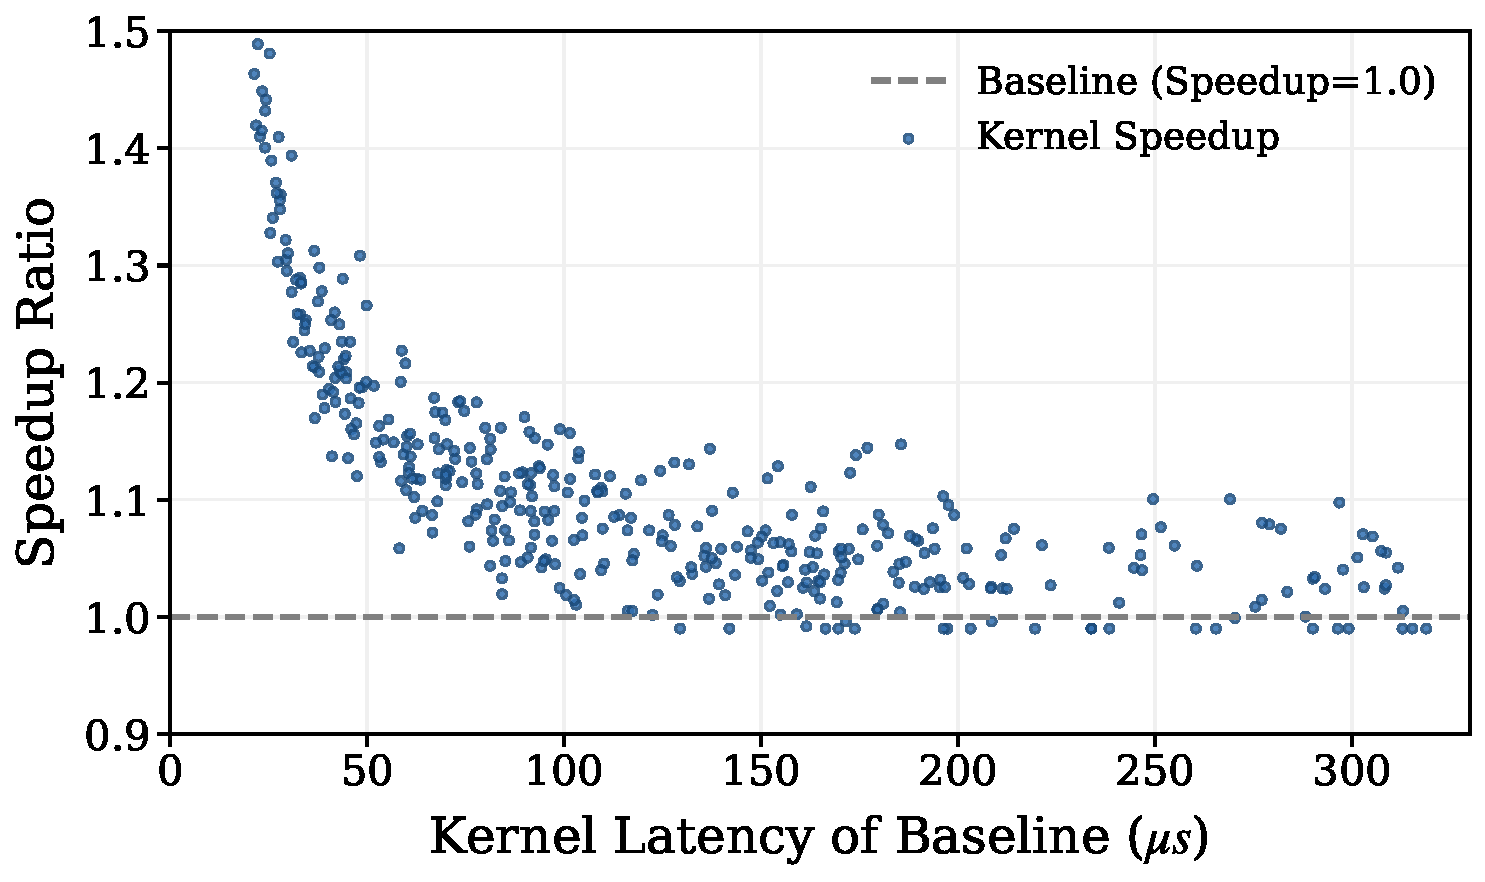
\includegraphics[width=\linewidth]{figures/evaluation/op-speedup/d_attn_execution_speedup.pdf}
		\caption{D-Attn}
	\end{subfigure}
	\hfill
	\begin{subfigure}[t]{0.40\textwidth}
		\centering
		\includegraphics[width=\linewidth]{figures/evaluation/op-speedup/mm_execution_speedup.pdf}
		\caption{MM}
	\end{subfigure}
	\caption{Kernel speedup versus Baseline device-kernel latency for D-Attn and MM. Blue points report the speedup of TilingInfer relative to Baseline.}
	\Description{Two scatter plots showing TilingInfer kernel speedup versus Baseline device-kernel latency for D-Attn and MM.}
	\label{fig:eval:op-scaling}
\end{figure*}
\DIFaddend 

\DIFdelbegin %DIFDELCMD < \label{sec:eval:analysis}
%DIFDELCMD < %%%
\DIFdelend \DIFaddbegin \FloatBarrier
\DIFaddend 

\DIFdelbegin \DIFdel{To gain deeper insight into the sources of performance gainsdemonstrated in \S\ref{sec:eval:result}, we analyze low-level hardware performance metrics collected during operator execution. }\DIFdelend \autoref{tab:performance_metrics} \DIFdelbegin \DIFdel{details the Speedup alongside key architectural metrics: Instruction Cache (I-Cache) Miss Rate, Scalar Instruction Ratio, Memory Access (Read \& Write) Ratios, and the final compiled Binary Size.
The }\textit{\DIFdel{Scalar Ratio}}%DIFAUXCMD
\DIFdel{, }\textit{\DIFdel{Memory Read Ratio}}%DIFAUXCMD
\DIFdel{, }\DIFdelend and \DIFdelbegin \textit{\DIFdel{Memory Write Ratio}} %DIFAUXCMD
\DIFdel{quantify the proportion of execution cycles of corresponding hardware units (scalar units, memory read/write units) relative to the total kernel execution cycles.
Comparing }\textbf{%DIFDELCMD < TilingInfer%%%
} %DIFAUXCMD
\DIFdel{(T) against the }\textbf{\DIFdel{Baseline}} %DIFAUXCMD
\DIFdel{(B) and }\textbf{\DIFdel{LLVM-spec}} %DIFAUXCMD
\DIFdel{(L), we attribute the improvements to two primary factors: reduced instruction fetch overhead and }\DIFdelend \DIFaddbegin \autoref{fig:eval:op-scaling} \DIFadd{show that }TilingInfer \DIFadd{does not produce uniform device-level gains; benefiting kernels fall into two mechanism-driven classes, whereas a third class is largely insensitive. For Upsample, D-Attn, FFN, and P-Attn, gains mainly arise because invariant propagation exposes constant branches and loop structure, enabling dead-code elimination and control-flow simplification; the resulting smaller instruction footprint reduces instruction-fetch and I-Cache pressure. A second class, including RMS, Pow, Gate, and GN, benefits primarily from }\DIFaddend simplified runtime calculation \DIFdelbegin \DIFdel{.
}%DIFDELCMD < 

%DIFDELCMD < %%%
\textit{\DIFdel{Reduction in Binary Size and I-Cache Misses.}}
%DIFAUXCMD
\DIFdel{By propagating runtime invariants, }\textbf{%DIFDELCMD < TilingInfer%%%
} %DIFAUXCMD
\DIFdel{enables the backend compiler to aggressively perform Dead Code Elimination (DCE) and simplify control flow graphs. This leads to significant binary size reductions: 34.0\% for }\texttt{\DIFdel{Upsample}}%DIFAUXCMD
\DIFdel{, 22.7\% for }\texttt{\DIFdel{D-Attn}}%DIFAUXCMD
\DIFdel{, 20.2\% for }\texttt{\DIFdel{FFN}}%DIFAUXCMD
\DIFdel{, and 14.8\% for }\texttt{\DIFdel{P-Attn}}%DIFAUXCMD
\DIFdel{. Consequently, the I-Cache Miss rate drops substantially: }\texttt{\DIFdel{Upsample}} %DIFAUXCMD
\DIFdel{(9.83\% $\rightarrow$ }\textbf{\DIFdel{0.12\%}}%DIFAUXCMD
\DIFdel{), }\texttt{\DIFdel{D-Attn}} %DIFAUXCMD
\DIFdel{(4.45\% $\rightarrow$ }\textbf{\DIFdel{0.18\%}}%DIFAUXCMD
\DIFdel{), }\texttt{\DIFdel{FFN}} %DIFAUXCMD
\DIFdel{(3.89\% $\rightarrow$ }\textbf{\DIFdel{0.15\%}}%DIFAUXCMD
\DIFdel{), }\DIFdelend \DIFaddbegin \DIFadd{and memory scheduling. Resolving loop bounds, offsets, }\DIFaddend and \DIFdelbegin \texttt{\DIFdel{P-Attn}} %DIFAUXCMD
\DIFdel{(16.40\% $\rightarrow$ 11.39\%). These improvements in instruction fetch efficiency contribute to the
observed speedups. }\DIFdelend \DIFaddbegin \DIFadd{schedule parameters removes scalar loads and address or control computations, exposes immediate operands, and enables access merging, loop unrolling, and more effective instruction scheduling. In contrast, Pool and Scat are largely insensitive: Pool is already compact with little instruction-fetch overhead, whereas Scat is dominated by memory work, so instruction-stream simplification does not shorten the critical path. Across all three classes, specialization mainly removes a roughly fixed amount of control and scheduling overhead. Its relative effect is therefore strongest for short-running kernels and diminishes as tensor computation or memory traffic dominates. The key determinant is not whether a parameter is static, but whether resolving it eliminates work on the kernel's performance-critical path.
}\DIFaddend 

\DIFdelbegin %DIFDELCMD < \begin{figure}[htbp]
%DIFDELCMD <     \centering
%DIFDELCMD <     \hfill
%DIFDELCMD <     \begin{minipage}{0.45\textwidth}
%DIFDELCMD <         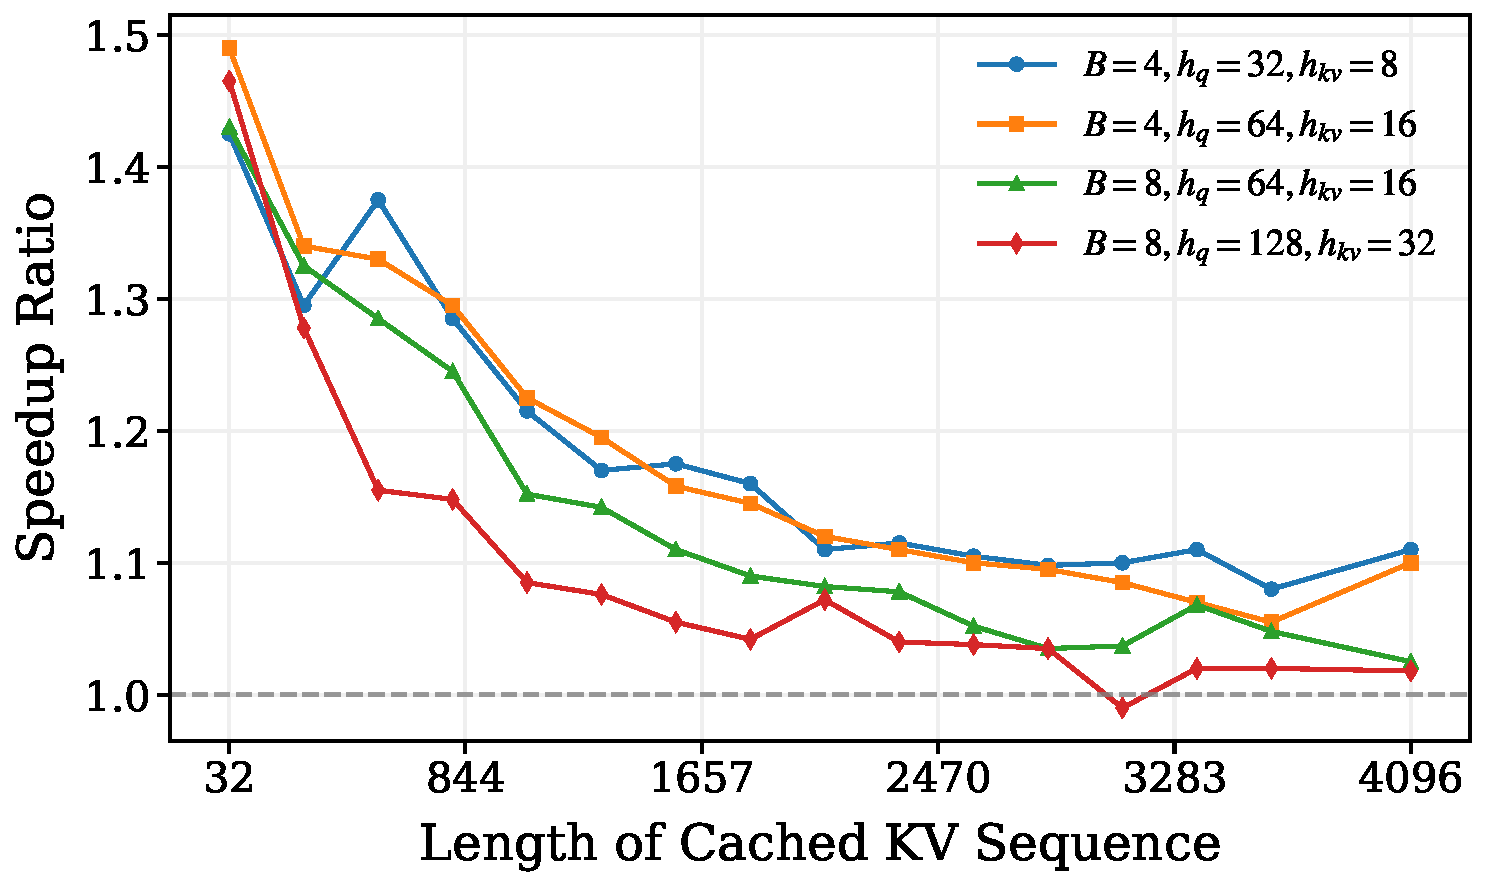
\includegraphics[width=\linewidth]{figures/evaluation/op-speedup/d_attn_kv_length_speedup.pdf}
%DIFDELCMD <         \caption{Speedup ratio of \texttt{D-Attn} under varying cached KV sequence lengths and configurations.}
%DIFDELCMD <         \Description{Line chart showing speedup ratio of D-Attn operator under different KV lengths.}
%DIFDELCMD <         \label{fig:eval:d_attn_kv}
%DIFDELCMD <         \vspace{-10pt}
%DIFDELCMD <     \end{minipage}
%DIFDELCMD <     \hfill
%DIFDELCMD <     \begin{minipage}{0.45\textwidth}
%DIFDELCMD <         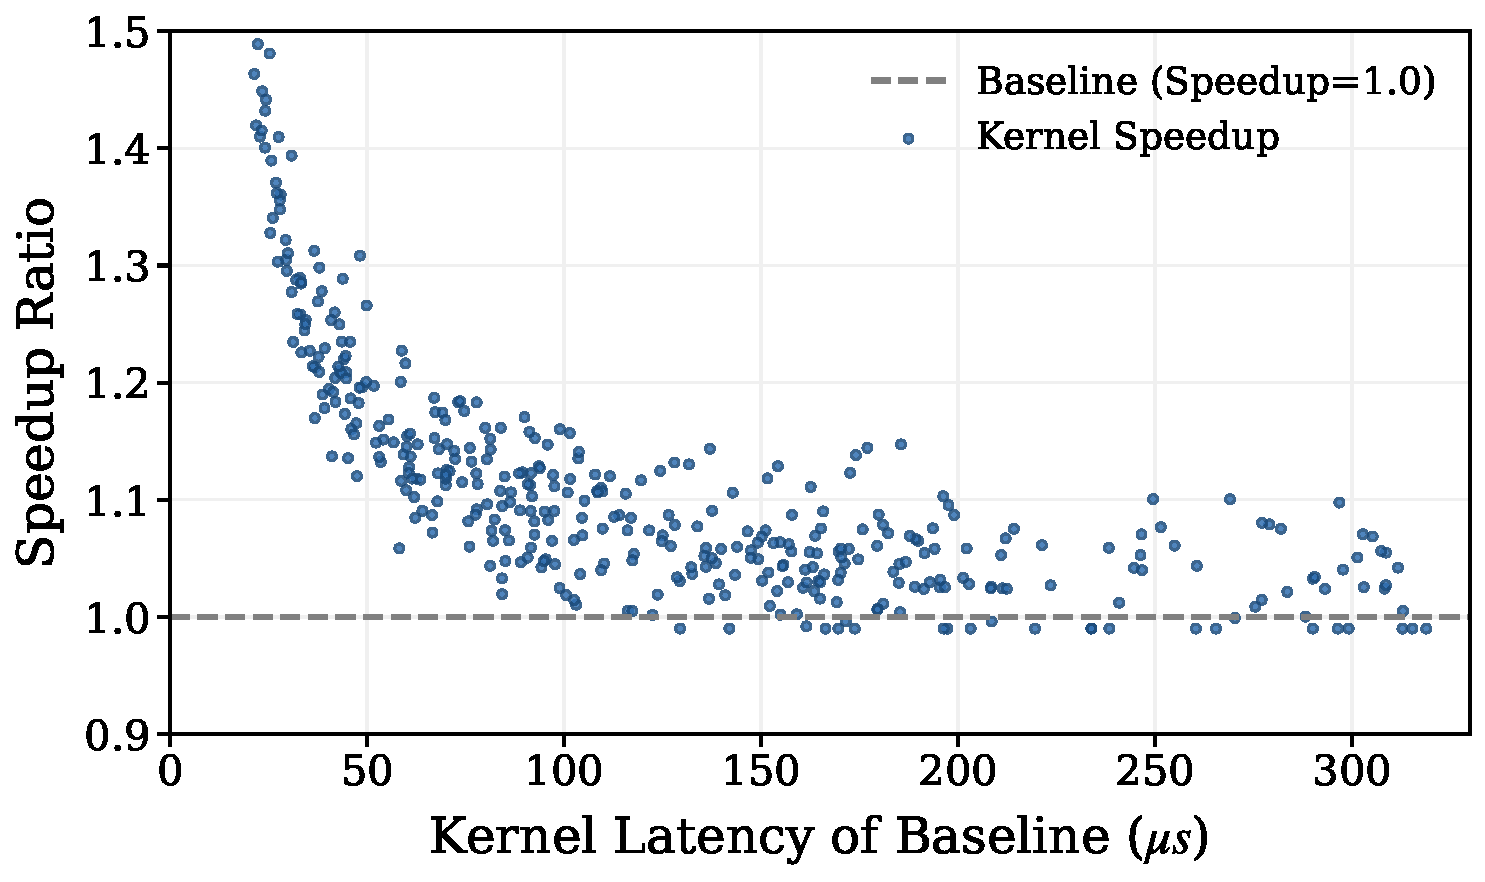
\includegraphics[width=\linewidth]{figures/evaluation/op-speedup/d_attn_execution_speedup.pdf}
%DIFDELCMD <         \caption{Distribution of speedup ratios of \textbf{TilingInfer} for the operator \texttt{D-Attn} relative to baseline kernel latency.}
%DIFDELCMD <         \Description{Scatter plot showing distribution of speedup ratios relative to baseline kernel latency.}
%DIFDELCMD <         \label{fig:eval:latency_dist}
%DIFDELCMD <         \vspace{-10pt}
%DIFDELCMD <     \end{minipage}
%DIFDELCMD <     \hfill
%DIFDELCMD < \end{figure}
%DIFDELCMD < %%%
\end{comment}
\subsection{Sensitivity to Resolved Schedule Parameters}
\label{sec:eval:sensitivity}

\begingroup
\setlength{\intextsep}{8pt}
\begin{figure}[t]
    \centering
    \begingroup
    % Keep these fills identical to GROUP_BACKGROUNDS in
    % plot_scripts/plot_resolved_tiling_sensitivity.py.
    \definecolor{controlflowbg}{HTML}{F8D7DA}
    \definecolor{addresscalcgbg}{HTML}{D9EAD3}
    \definecolor{mmschedulebg}{HTML}{DDEBF7}
    \newcommand{\controlmath}[1]{{\setlength{\fboxsep}{1.0pt}%
        \colorbox{controlflowbg}{\strut\ensuremath{#1}}}}
    \newcommand{\addressmath}[1]{{\setlength{\fboxsep}{1.0pt}%
        \colorbox{addresscalcgbg}{\strut\ensuremath{#1}}}}
    \newcommand{\schedulemath}[1]{{\setlength{\fboxsep}{1.0pt}%
        \colorbox{mmschedulebg}{\strut\ensuremath{#1}}}}
    \newcommand{\auxfn}[1]{{\sffamily\bfseries #1}}
    \newcommand{\controlgroup}[1]{{\setlength{\fboxsep}{1.5pt}%
        \colorbox{controlflowbg}{\parbox{0.91\linewidth}{#1}}}}
    \newcommand{\addressgroup}[1]{{\setlength{\fboxsep}{1.5pt}%
        \colorbox{addresscalcgbg}{\parbox{0.91\linewidth}{#1}}}}
    \newcommand{\schedulegroup}[1]{{\setlength{\fboxsep}{1.5pt}%
        \colorbox{mmschedulebg}{\parbox{0.91\linewidth}{#1}}}}

    \begin{minipage}[t]{0.405\linewidth}
        \fontsize{5.45}{6.05}\selectfont
        \setlength{\fboxsep}{3pt}
        \fcolorbox{black!30}{white}{%
        \parbox[t][0.72in][t]{0.92\linewidth}{%
            \centering
            \textbf{(a) D-Attn \(\mathrm{Query}\times\mathrm{Key}^{\mathsf T}\)}\par
            \vspace{1pt}
            \(\displaystyle
            \mathrm{Output}_{b,h}
              =\mathrm{Query}_{b,h}\mathrm{Key}_{b,h}^{\mathsf T}
            \)\par
            \vspace{1pt}
            \raggedright
            \(\mathrm{Query}_{b,h}:[1,D_{head}]\): Query row of attention
            head \(h\) for request \(b\) in the batch.\par
            \(\mathrm{Key}_{b,h}:[T_b,D_{head}]\): cached Key rows of
            attention head \(h\) for request \(b\) in the batch.\par
            \(\mathbf{T}=[T_0,\ldots,T_{B-1}]\): per-request KV lengths
            (runtime input).
        }}\par
        \vspace{3pt}
        \fontsize{5.05}{5.50}\selectfont
        \fcolorbox{black!30}{white}{%
        \parbox[t][1.15in][t]{0.92\linewidth}{%
            \centering
            \textbf{(b) Representative schedule parameters for
                \(\mathrm{Query}\times\mathrm{Key}^{\mathsf T}\)}(34 total)\par
            \vspace{2pt}
            \raggedright
            \controlgroup{%
                \centering
                \textbf{Control logic (6 total)}\par
                \raggedright
                \(T_N\): Key rows in one output tile.\\
                \(P\): Key rows in one cache page.\\
                \(T_D\): Key columns in one narrow load.
            }\par
            \vspace{1pt}
            \addressgroup{%
                \centering
                \textbf{Per-core tile dimensions/addressing
                (14 total)}\par
                \raggedright
                \(M_c\): Output-row extent assigned to one core.\\
                \(K_c\): Reduction-column extent assigned to one core.
            }\par
            \vspace{1pt}
            \schedulegroup{%
                \centering
                \textbf{Core-loop scheduling/memory resources
                (14 total)}\par
                \raggedright
                \(N_c\): Number of active compute cores.\\
                \(n_K\): Number of Key buffers.
            }
        }}
    \end{minipage}\hfill
    \begin{minipage}[t]{0.575\linewidth}
        \fontsize{4.80}{5.20}\selectfont
        \setlength{\fboxsep}{3pt}
        \fcolorbox{black!30}{white}{%
        \parbox[t][2.10in][t]{0.94\linewidth}{%
            \centering
            \textbf{(c) Tiled BMM pseudocode for
                \(\mathrm{Query}\times\mathrm{Key}^{\mathsf T}\)}\par
            \vspace{2pt}
            \raggedright
            \ttfamily
            \begin{tabular}{@{}>{\color{black!55}}r@{\hspace{3pt}}l@{}}
             1 & \textbf{function} \auxfn{BMM}(Query, Key, \(\mathbf{T}\);
                 \(\controlmath{T_N},\controlmath{P},\controlmath{T_D},
                 \addressmath{M_c},\addressmath{K_c},
                 \schedulemath{N_c},\schedulemath{n_K}\)) \\
             2 & \quad configure \(\schedulemath{N_c}\) cores and
                 \(\schedulemath{n_K}\) Key buffers \\
             3 & \quad\textbf{parallel for} \(c=0,\ldots,\schedulemath{N_c}-1\) \\
             4 & \quad\quad\textbf{for} tile \(\tau\) with
                 \(\controlmath{T_N}\) Key rows \(\times\)
                 \(\addressmath{K_c}\) columns assigned to core \(c\) \\
             5 & \quad\quad\quad \textit{// \(n_0\): first Key row;
                 \(k_0\): first reduction column; \(T_b\): request \(b\)'s KV length} \\
             6 & \quad\quad\quad
                 \((b,h,n_0,k_0)\leftarrow
                 \text{\auxfn{TileOffset}}(\tau;\addressmath{M_c},
                 \controlmath{T_N},\addressmath{K_c},\mathbf{T})\) \\
             7 & \quad\quad\quad
                 \(n\leftarrow\min(\controlmath{T_N},T_b-n_0)\) \\
             8 & \quad\quad\quad \textbf{for} \((p,r,u)\) in
                 \auxfn{PageFragments}\((\mathrm{Key},b,n_0,n;\controlmath{P})\) \\
             9 & \quad\quad\quad\quad\textbf{if}
                 \(\controlmath{T_N}=\controlmath{P}\) \\
            10 & \quad\quad\quad\quad\quad
                 one-copy load Key\([p,r:r+u,h,k_0:k_0+\addressmath{K_c}]\)
                 \(\rightarrow\mathrm{KeyBuf[next(}\schedulemath{n_K}\mathrm{)]}\) \\
            11 & \quad\quad\quad\quad\textbf{else}
                 \(\;(\controlmath{T_N}\ne\controlmath{P})\) \\
            12 & \quad\quad\quad\quad\quad\textbf{for}
                 \(d_0=k_0,k_0+\controlmath{T_D},\ldots,
                 k_0+\addressmath{K_c}\) \\
            13 & \quad\quad\quad\quad\quad\quad
                 append load Key\([p,r:r+u,h,d_0:d_0+\controlmath{T_D}]\)
                 \(\rightarrow\mathrm{KeyBuf[next(}\schedulemath{n_K}\mathrm{)]}\) \\
            14 & \quad\quad\quad
                 load Query\([b,0,h,k_0:k_0+\addressmath{K_c}]\)
                 \(\rightarrow\mathrm{QueryBuf}\) \\
            15 & \quad\quad\quad Output\(_{\rm tile}\mathrel{+}=\)
                 \auxfn{MMAD}(QueryBuf, KeyBuf)
            \end{tabular}
            \vspace{3pt}\par
            \rmfamily
            \auxfn{TileOffset}: maps tile \(\tau\) to start coordinate
            \((b,h,n_0,k_0)\): request, head, Key row, and reduction column.\par
            \auxfn{PageFragments}: resolves \(n\) logical Key rows through the
            page table as non-crossing fragments \((p,r,u)\).\par
            \auxfn{MMAD}: multiplies QueryBuf by KeyBuf and accumulates the
            partial result into Output\(_{\rm tile}\).
        }}
    \end{minipage}

    \caption{Tiled D-Attn BMM. Panel (b) lists seven representative
    schedule parameters; the three groups contain 6, 14, and 14 schedule
    parameters in total. Matching backgrounds in panel (c) mark their use
    sites and correspond to the groups evaluated in
    \autoref{fig:eval:constant-sensitivity}.}
    \Description{Three panels. Panel (a) defines the per-request Query--Key
    multiplication, explains the Query and Key tensors for request and head
    indices, and defines the runtime array of per-request KV lengths. Panel
    (b) lists seven representative schedule parameters and gives total
    counts of 6, 14, and 14 schedule parameters for Control logic, Per-core tile
    dimensions/addressing, and Core-loop scheduling/memory resources,
    respectively. Panel (c) takes all seven schedule
    parameters as inputs and shows core configuration, per-core tile indexing,
    page-aware Key loading with separate T-N-equals-P and T-N-not-equals-P
    paths, and the final tiled matrix multiplication.}
    \label{fig:resolved-tiling-code}
    \endgroup
\end{figure}


\begin{figure}[t]
	\centering
	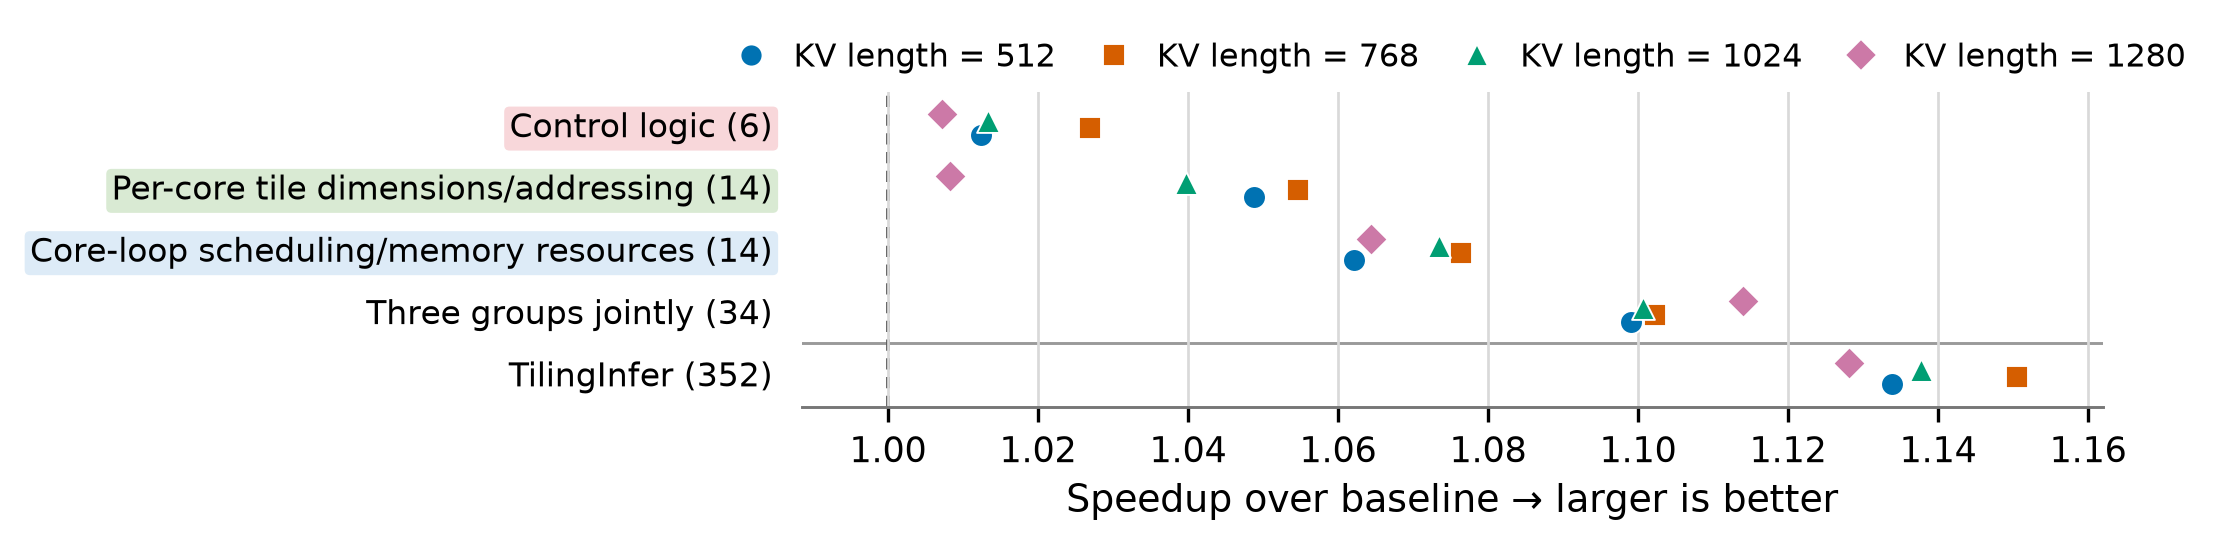
\includegraphics[width=0.85\textwidth]{figures/evaluation/op-speedup/resolved_constant_sensitivity.pdf}
	\caption{Sensitivity to resolved schedule parameters across runtime
	shapes. Numbers in parentheses give the number of specialized schedule
	parameters. Each point shows the speedup at one KV length; the first three
	label backgrounds match the groups in
	\autoref{fig:resolved-tiling-code}.}
	\Description{Point plot of speedup over Baseline for Control logic with 6
	specialized parameters, Per-core tile dimensions/addressing with 14,
	Core-loop scheduling/memory resources with 14, the three groups jointly
	with 34, and TilingInfer with 304.
	Each row contains separate points for KV lengths 512, 768, 1024, and 1280,
	and no error bars.}
	\label{fig:eval:constant-sensitivity}
\end{figure}
\endgroup

{\color{blue}%
This section analyzes whether specializing different groups of schedule parameters yields different benefits: can one group provide a substantially larger gain than the others?
\par}

{\color{blue}%
For D-Attn, $\mathrm{Query}_{b,h}\mathrm{Key}_{b,h}^{\mathsf T}$ multiplies the Query row of request $b$ and attention head $h$ by its cached Key rows, while $\mathbf{T}$ stores each request's KV length. Its 34 schedule parameters form Control logic (6), Per-core tile dimensions/addressing (14), and Core-loop scheduling/memory resources (14). Control logic covers the branches and loop bounds that select how Key data are loaded. Per-core tile dimensions/addressing specifies how much work each core owns and maps tile indices to tensor addresses. Core-loop scheduling/memory resources controls how tiles are assigned to active cores and how on-chip buffers are allocated and reused inside the core loop. \autoref{fig:resolved-tiling-code}(b) lists seven representative examples. In panel (c), $T_N$ and $K_c$ split Key rows and reduction columns into tiles, while $M_c$ and $N_c$ distribute the tiles to cores. TileOffset uses these extents and $\mathbf{T}$ to recover $(b,h,n_0,k_0)$, the tile's starting coordinate. The schedule parameters $T_N$, $P$, and $T_D$ select one page-aligned load or several narrow page-table loads, while $n_K$ selects the Key buffer. BMM then loads the matching Query slice and computes the tile.
\par}

{\color{blue}%
Overall, \autoref{fig:eval:constant-sensitivity} shows that specialization value depends more on a parameter's use site than on parameter count. Across KV lengths 512--1280, the 14 Core-loop scheduling/memory-resource parameters achieve the largest isolated geometric-mean speedup, 1.07$\times$, by configuring per-core work and Key-buffer resources on the inner BMM path. The 14 Per-core tile dimension/addressing parameters reach 1.04$\times$, while the 6 Control-logic parameters reach 1.02$\times$. Thus, count alone poorly predicts specialization value.
\par}

{\color{blue}%
The three isolated gains sum to 12.2\%, whereas jointly specializing all 34 parameters yields 1.10$\times$ (10.4\%), or 85.0\% of that sum, indicating interaction and diminishing returns. TilingInfer specializes 304 stable parameters and reaches 1.14$\times$. Although the 34 $\mathrm{Query}\times\mathrm{Key}^{\mathsf T}$ parameters comprise only 11.0\% of these fields, they recover 75.0\% of the full gain; the remaining 270 add only 3.4 percentage points. Because these 34 parameters control D-Attn's core BMM in \autoref{fig:resolved-tiling-code}(c), specializing its hot-path address and control flow is more valuable than resolving constants on colder paths.
\par}

\begin{comment}
\DIFdelend \DIFaddbegin \subsection{\DIFadd{Sensitivity to Resolved Schedule Parameters}}
\label{sec:eval:sensitivity}
\DIFaddend 

\DIFdelbegin \textit{\DIFdel{Optimization of Computational Intensity and Memory Schedule.}}
%DIFAUXCMD
\textbf{%DIFDELCMD < TilingInfer%%%
} %DIFAUXCMD
\DIFdel{substantially reduces the Scalar Ratio for operators like }\texttt{\DIFdel{RMS}} %DIFAUXCMD
\DIFdel{(97.9\% $\rightarrow$ 88.6\%) }\DIFdelend \DIFaddbegin \begingroup
\setlength{\intextsep}{6pt}
\begin{figure}[H]
    \centering
    \begingroup
    % Keep these fills identical to GROUP_BACKGROUNDS in
    % plot_scripts/plot_resolved_tiling_sensitivity.py.
    \definecolor{controlflowbg}{HTML}{F8D7DA}
    \definecolor{addresscalcgbg}{HTML}{D9EAD3}
    \definecolor{mmschedulebg}{HTML}{DDEBF7}
    \newcommand{\controlmath}[1]{{\setlength{\fboxsep}{1.0pt}%
        \colorbox{controlflowbg}{\strut\ensuremath{#1}}}}
    \newcommand{\addressmath}[1]{{\setlength{\fboxsep}{1.0pt}%
        \colorbox{addresscalcgbg}{\strut\ensuremath{#1}}}}
    \newcommand{\schedulemath}[1]{{\setlength{\fboxsep}{1.0pt}%
        \colorbox{mmschedulebg}{\strut\ensuremath{#1}}}}
    \newcommand{\auxfn}[1]{{\sffamily\bfseries #1}}
    \newcommand{\controlgroup}[1]{{\setlength{\fboxsep}{1.5pt}%
        \colorbox{controlflowbg}{\parbox{0.91\linewidth}{#1}}}}
    \newcommand{\addressgroup}[1]{{\setlength{\fboxsep}{1.5pt}%
        \colorbox{addresscalcgbg}{\parbox{0.91\linewidth}{#1}}}}
    \newcommand{\schedulegroup}[1]{{\setlength{\fboxsep}{1.5pt}%
        \colorbox{mmschedulebg}{\parbox{0.91\linewidth}{#1}}}}

    \begin{minipage}[t]{0.405\linewidth}
        \fontsize{5.45}{6.05}\selectfont
        \setlength{\fboxsep}{3pt}
        \fcolorbox{black!30}{white}{%
        \parbox[t][0.72in][t]{0.92\linewidth}{%
            \centering
            \textbf{(a) D-Attn \(\mathrm{Query}\times\mathrm{Key}^{\mathsf T}\)}\par
            \vspace{1pt}
            \(\displaystyle
            \mathrm{Output}_{b,h}
              =\mathrm{Query}_{b,h}\mathrm{Key}_{b,h}^{\mathsf T}
            \)\par
            \vspace{1pt}
            \raggedright
            \(\mathrm{Query}_{b,h}:[1,D_{head}]\): Query row of attention
            head \(h\) for request \(b\) in the batch.\par
            \(\mathrm{Key}_{b,h}:[T_b,D_{head}]\): cached Key rows of
            attention head \(h\) for request \(b\) in the batch.\par
            \(\mathbf{T}=[T_0,\ldots,T_{B-1}]\): per-request KV lengths
            (runtime input).
        }}\par
        \vspace{3pt}
        \fontsize{5.05}{5.50}\selectfont
        \fcolorbox{black!30}{white}{%
        \parbox[t][1.15in][t]{0.92\linewidth}{%
            \centering
            \textbf{(b) Representative schedule parameters for
                \(\mathrm{Query}\times\mathrm{Key}^{\mathsf T}\)}(34 total)\par
            \vspace{2pt}
            \raggedright
            \controlgroup{%
                \centering
                \textbf{Control logic (6 total)}\par
                \raggedright
                \(T_N\): Key rows in one output tile.\\
                \(P\): Key rows in one cache page.\\
                \(T_D\): Key columns in one narrow load.
            }\par
            \vspace{1pt}
            \addressgroup{%
                \centering
                \textbf{Per-core tile dimensions/addressing
                (14 total)}\par
                \raggedright
                \(M_c\): Output-row extent assigned to one core.\\
                \(K_c\): Reduction-column extent assigned to one core.
            }\par
            \vspace{1pt}
            \schedulegroup{%
                \centering
                \textbf{Core-loop scheduling/memory resources
                (14 total)}\par
                \raggedright
                \(N_c\): Number of active compute cores.\\
                \(n_K\): Number of Key buffers.
            }
        }}
    \end{minipage}\hfill
    \begin{minipage}[t]{0.575\linewidth}
        \fontsize{4.80}{5.20}\selectfont
        \setlength{\fboxsep}{3pt}
        \fcolorbox{black!30}{white}{%
        \parbox[t][2.10in][t]{0.94\linewidth}{%
            \centering
            \textbf{(c) Tiled BMM pseudocode for
                \(\mathrm{Query}\times\mathrm{Key}^{\mathsf T}\)}\par
            \vspace{2pt}
            \raggedright
            \ttfamily
            \begin{tabular}{@{}>{\color{black!55}}r@{\hspace{3pt}}l@{}}
             1 & \textbf{function} \auxfn{BMM}(Query, Key, \(\mathbf{T}\);
                 \(\controlmath{T_N},\controlmath{P},\controlmath{T_D},
                 \addressmath{M_c},\addressmath{K_c},
                 \schedulemath{N_c},\schedulemath{n_K}\)) \\
             2 & \quad configure \(\schedulemath{N_c}\) cores and
                 \(\schedulemath{n_K}\) Key buffers \\
             3 & \quad\textbf{parallel for} \(c=0,\ldots,\schedulemath{N_c}-1\) \\
             4 & \quad\quad\textbf{for} tile \(\tau\) with
                 \(\controlmath{T_N}\) Key rows \(\times\)
                 \(\addressmath{K_c}\) columns assigned to core \(c\) \\
             5 & \quad\quad\quad \textit{// \(n_0\): first Key row;
                 \(k_0\): first reduction column; \(T_b\): request \(b\)'s KV length} \\
             6 & \quad\quad\quad
                 \((b,h,n_0,k_0)\leftarrow
                 \text{\auxfn{TileOffset}}(\tau;\addressmath{M_c},
                 \controlmath{T_N},\addressmath{K_c},\mathbf{T})\) \\
             7 & \quad\quad\quad
                 \(n\leftarrow\min(\controlmath{T_N},T_b-n_0)\) \\
             8 & \quad\quad\quad \textbf{for} \((p,r,u)\) in
                 \auxfn{PageFragments}\((\mathrm{Key},b,n_0,n;\controlmath{P})\) \\
             9 & \quad\quad\quad\quad\textbf{if}
                 \(\controlmath{T_N}=\controlmath{P}\) \\
            10 & \quad\quad\quad\quad\quad
                 one-copy load Key\([p,r:r+u,h,k_0:k_0+\addressmath{K_c}]\)
                 \(\rightarrow\mathrm{KeyBuf[next(}\schedulemath{n_K}\mathrm{)]}\) \\
            11 & \quad\quad\quad\quad\textbf{else}
                 \(\;(\controlmath{T_N}\ne\controlmath{P})\) \\
            12 & \quad\quad\quad\quad\quad\textbf{for}
                 \(d_0=k_0,k_0+\controlmath{T_D},\ldots,
                 k_0+\addressmath{K_c}\) \\
            13 & \quad\quad\quad\quad\quad\quad
                 append load Key\([p,r:r+u,h,d_0:d_0+\controlmath{T_D}]\)
                 \(\rightarrow\mathrm{KeyBuf[next(}\schedulemath{n_K}\mathrm{)]}\) \\
            14 & \quad\quad\quad
                 load Query\([b,0,h,k_0:k_0+\addressmath{K_c}]\)
                 \(\rightarrow\mathrm{QueryBuf}\) \\
            15 & \quad\quad\quad Output\(_{\rm tile}\mathrel{+}=\)
                 \auxfn{MMAD}(QueryBuf, KeyBuf)
            \end{tabular}
            \vspace{3pt}\par
            \rmfamily
            \auxfn{TileOffset}: maps tile \(\tau\) to start coordinate
            \((b,h,n_0,k_0)\): request, head, Key row, and reduction column.\par
            \auxfn{PageFragments}: resolves \(n\) logical Key rows through the
            page table as non-crossing fragments \((p,r,u)\).\par
            \auxfn{MMAD}: multiplies QueryBuf by KeyBuf and accumulates the
            partial result into Output\(_{\rm tile}\).
        }}
    \end{minipage}

    \caption{Tiled D-Attn BMM. Panel (b) lists seven representative
    schedule parameters; the three groups contain 6, 14, and 14 schedule
    parameters in total. Matching backgrounds in panel (c) mark their use
    sites and correspond to the groups evaluated in
    \autoref{fig:eval:constant-sensitivity}.}
    \Description{Three panels. Panel (a) defines the per-request Query--Key
    multiplication, explains the Query and Key tensors for request and head
    indices, and defines the runtime array of per-request KV lengths. Panel
    (b) lists seven representative schedule parameters and gives total
    counts of 6, 14, and 14 schedule parameters for Control logic, Per-core tile
    dimensions/addressing, and Core-loop scheduling/memory resources,
    respectively. Panel (c) takes all seven schedule
    parameters as inputs and shows core configuration, per-core tile indexing,
    page-aware Key loading with separate T-N-equals-P and T-N-not-equals-P
    paths, and the final tiled matrix multiplication.}
    \label{fig:resolved-tiling-code}
    \endgroup
\end{figure}


\begin{figure}[H]
	\centering
	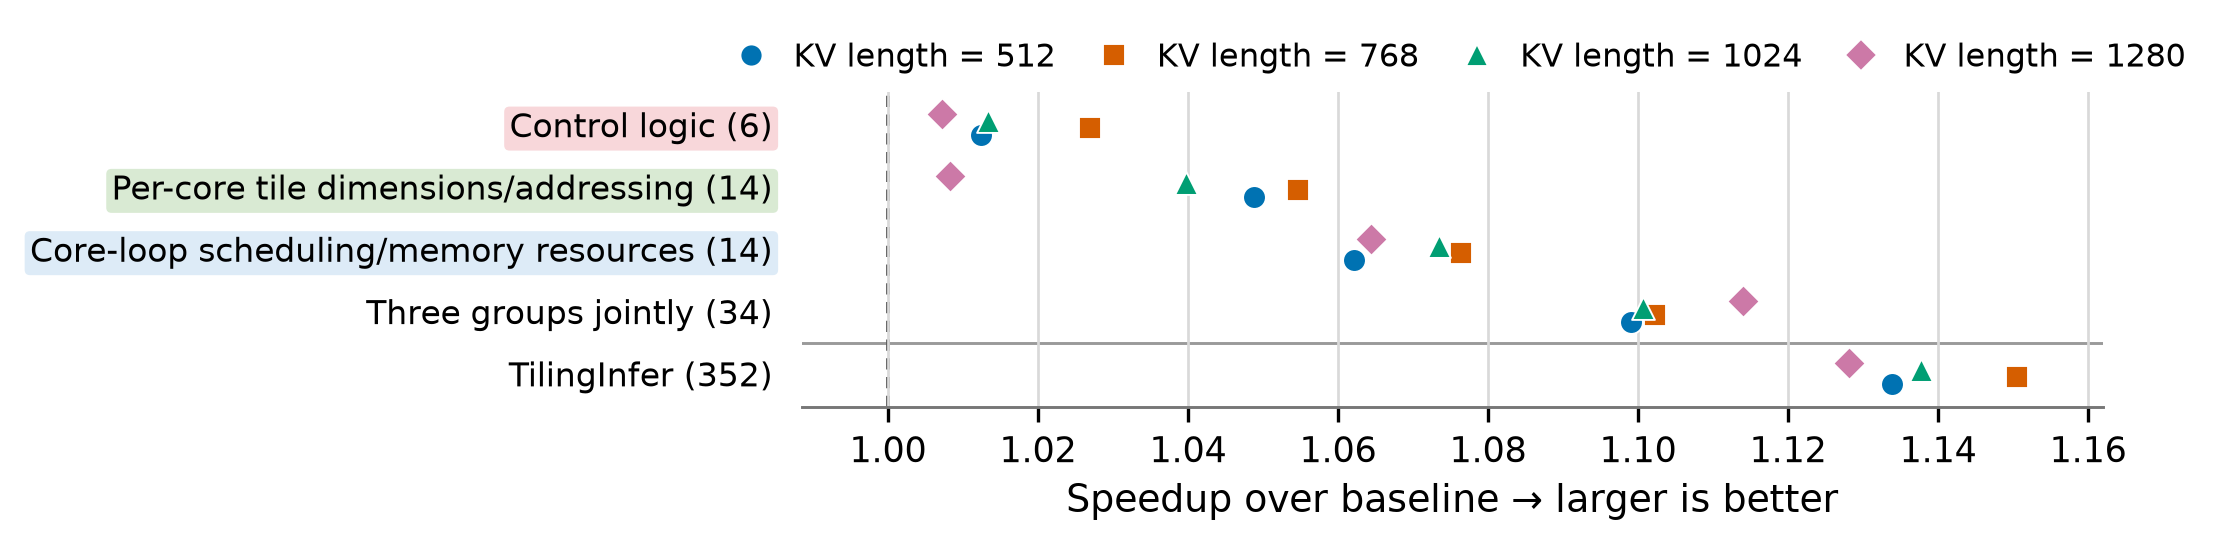
\includegraphics[width=0.85\textwidth]{figures/evaluation/op-speedup/resolved_constant_sensitivity.pdf}
	\caption{Sensitivity to resolved schedule parameters across runtime
	shapes. Numbers in parentheses give the number of specialized schedule
	parameters. Each point shows the speedup at one KV length; the first three
	label backgrounds match the groups in
	\autoref{fig:resolved-tiling-code}.}
	\Description{Point plot of speedup over Baseline for Control logic with 6
	specialized parameters, Per-core tile dimensions/addressing with 14,
	Core-loop scheduling/memory resources with 14, the three groups jointly
	with 34, and TilingInfer with 304.
	Each row contains separate points for KV lengths 512, 768, 1024, and 1280,
	and no error bars.}
	\label{fig:eval:constant-sensitivity}
\end{figure}
\endgroup

\DIFadd{This section analyzes whether specializing different groups of schedule
parameters yields different benefits: can one group provide a substantially
larger gain than the others?
}

\DIFadd{For D-Attn, $\mathrm{Query}_{b,h}\mathrm{Key}_{b,h}^{\mathsf T}$
multiplies the Query row of request $b$ and attention head $h$ by its cached
Key rows, while $\mathbf{T}$ stores each request's KV length. Its 34 schedule
parameters form Control logic (6), Per-core tile dimensions/addressing (14),
}\DIFaddend and \DIFdelbegin \texttt{\DIFdel{Pow}} %DIFAUXCMD
\DIFdel{(59.5\% $\rightarrow$ 53.1\%), confirming that resolving loop bounds and offsets at compile-time effectively converts runtime scalar calculations into immediate operands.
The Memory Read Ratio also improves,
dropping from 25.0\% to 16.4\% for }\texttt{\DIFdel{Gate}} %DIFAUXCMD
\DIFdel{and from 25.0\% to 18.8\% for }\texttt{\DIFdel{GN}}%DIFAUXCMD
\DIFdel{. This reduction is primarily due to the decreased number of parameters read from device memory, as well as the compiler's ability to merge multiple memory accesses when loop iteration counts are determined at compile time. Furthermore, optimizations such as loop unrolling can facilitate instruction scheduling and effectively hide memory access latency. These factors collectively contribute to the speedups observed in operators such as }\texttt{\DIFdel{D-Attn}}%DIFAUXCMD
\DIFdelend \DIFaddbegin \DIFadd{Core-loop scheduling/memory resources (14). Control logic covers the
branches and loop bounds that select how Key data are loaded. Per-core tile
dimensions/addressing specifies how much work each core owns and maps tile
indices to tensor addresses. Core-loop scheduling/memory resources controls
how tiles are assigned to active cores and how on-chip buffers are allocated
and reused inside the core loop.
}\autoref{fig:resolved-tiling-code}\DIFadd{(b) lists seven representative examples. In
panel (c), $T_N$ and $K_c$ split Key rows and reduction columns into tiles,
while $M_c$ and $N_c$ distribute the tiles to cores. TileOffset uses these
extents and $\mathbf{T}$ to recover $(b,h,n_0,k_0)$, the tile's starting
coordinate. The schedule parameters $T_N$}\DIFaddend , \DIFdelbegin \texttt{\DIFdel{Pow}}%DIFAUXCMD
\DIFdel{, and }\texttt{\DIFdel{RMS}}%DIFAUXCMD
\DIFdelend \DIFaddbegin \DIFadd{$P$, and $T_D$ select one page-aligned load
or several narrow page-table loads, while $n_K$ selects the Key buffer. BMM
then loads the matching Query slice and computes the tile}\DIFaddend .

\DIFdelbegin \textit{\DIFdel{Insensitive Operators.}}
%DIFAUXCMD
\DIFdel{Some operators, such as }\texttt{\DIFdel{Pool}} %DIFAUXCMD
\DIFdel{and }\texttt{\DIFdel{Scat}}%DIFAUXCMD
\DIFdel{, show negligible speedups (1.00}\DIFdelend \DIFaddbegin \DIFadd{Overall, }\autoref{fig:eval:constant-sensitivity} \DIFadd{shows that specialization
value depends more on a parameter's use site than on parameter count. Across KV
lengths 512--1280, the 14 Core-loop scheduling/memory-resource parameters
achieve the largest isolated geometric-mean speedup, 1.07}\DIFaddend $\times$\DIFdelbegin \DIFdel{$\sim$ 1.01}\DIFdelend \DIFaddbegin \DIFadd{, by
configuring per-core work and Key-buffer resources on the inner BMM path. The
14 Per-core tile dimension/addressing parameters reach 1.04$\times$, while the
6 Control-logic parameters reach 1.02}\DIFaddend $\times$\DIFdelbegin \DIFdel{). For }\texttt{\DIFdel{Pool}}%DIFAUXCMD
\DIFdel{, the }\textbf{\DIFdel{Baseline}} %DIFAUXCMD
\DIFdel{binary size is already minimal (13.35KB)with 0.08\% I-Cache miss rate, leaving no room for control flow simplification. For }\texttt{\DIFdel{Scat}}%DIFAUXCMD
\DIFdel{, the overhead of scalar instructions and instruction fetching is minimal compared to memory-bound operations. Optimizations in the instruction stream do not translate into visible latency reductions when the bottleneck lies in memory or arithmetic units.
}\DIFdelend \DIFaddbegin \DIFadd{. Thus, count alone poorly
predicts specialization value.
}\DIFaddend 

\DIFdelbegin \textit{\DIFdel{Impact of Workload Scale.}}
%DIFAUXCMD
%DIFDELCMD < \autoref{fig:eval:d_attn_kv} %%%
\DIFdel{and }%DIFDELCMD < \autoref{fig:eval:latency_dist} %%%
\DIFdel{show that speedup decreases towards 1.0 as workload increases. This implies that performance benefits from kernel specialization are relatively fixed in absolute time.
Consequently, this fixed reduction yields significant speedup ratios for small-scale kernels but becomes negligible for heavy workloads dominated by computation and memory access}\DIFdelend \DIFaddbegin \DIFadd{The three isolated gains sum to 12.2\%, whereas jointly specializing all 34
parameters yields 1.10$\times$ (10.4\%), or 85.0\% of that sum, indicating
interaction and diminishing returns. }TilingInfer \DIFadd{specializes 304 stable parameters
and reaches 1.14$\times$. Although the 34
$\mathrm{Query}\times\mathrm{Key}^{\mathsf T}$ parameters comprise only 11.0\%
of these fields, they recover 75.0\% of the full gain; the remaining 270 add
only 3.4 percentage points. Because these 34 parameters control D-Attn's core
BMM in }\autoref{fig:resolved-tiling-code}\DIFadd{(c), specializing its hot-path address
and control flow is more valuable than resolving constants on colder paths}\DIFaddend .

%DIF <  \textit{Analysis on the compilation pipelines of the kernel specialization}
\DIFdelbegin %DIFDELCMD < 

%DIFDELCMD < %%%
%DIF <  TODO:
%DIF <  绘制几种算子启动kernel特化后的 IR 指令数目随pass执行的变化情况，其中只标注 JIT spec pass
\end{comment}
\subsection{Binary-Size Trade-off}
\label{sec:eval:tradeoff}

\noindent
\hfill
\begin{adjustbox}{valign=t,minipage=0.72\textwidth}
	\color{black}
\centering
\includegraphics[width=\linewidth]{figures/evaluation/op-reduction/flashinfer_archive_breakdown.pdf}
\captionsetup{hypcap=false,skip=2pt}
\captionof{figure}{Full AOT archive breakdown.}
\Description{Breakdown of the full AOT archive into Prefill, Decode, Mamba SSU, and Utility.}
\label{fig:eval:flashinfer-tradeoff-archive}

\end{adjustbox}
\hfill
\mbox{}

\noindent
\hfill
\begin{adjustbox}{valign=t,minipage=0.95\textwidth}
	\centering
	\includegraphics[width=\linewidth]{figures/evaluation/op-reduction/flashinfer_footprint.pdf}
	\captionsetup{hypcap=false,skip=3pt}
	\captionof{figure}{Per-model FlashInfer footprint.}
	\Description{Stacked horizontal bars showing specialized FlashInfer library sizes for 17 model variants.}
	\label{fig:eval:flashinfer-tradeoff-footprint}
\end{adjustbox}
\hfill
\mbox{}
\par\kern8pt

{\color{red}%
\DIFdel{%
We adapted TilingInfer to eliminate redundant template instantiations never called at runtime. We targeted FlashInfer~}\cite{ye2025flashinfer}\DIFdel{, a state-of-the-art attention kernel library widely used in LLM serving systems like vLLM and SGLang. The results of this optimization are presented in the original GPU binary-reduction table. We evaluated the binary size reduction for different LLM families (Llama and Qwen) with various model sizes. TilingInfer demonstrates remarkable effectiveness in eliminating redundant code, reducing the binary size of the FlashInfer library from approximately 520MB to roughly 20MB. On average, TilingInfer achieves a 96.2\% reduction in binary size. This substantial reduction in library footprint benefits cold-start-sensitive scenarios such as serverless ML inference, where loading large operator libraries into GPU memory constitutes a major portion of initialization latency. Other DSA architectures with AoT-compiled operator libraries that suffer from similar code-bloat issues could also benefit from TilingInfer.
}
\par}

{\color{blue}%
We apply path-liveness information to FlashInfer and retain the shared objects reachable by each of 17 model variants, including standard, FP8 KV-cache, MoE, sliding-window, and logits-soft-cap attention as well as Mamba Selective-State-Update (SSU) kernels. The universal AOT archive contains 247 shared objects and occupies 542\,MB. As shown in \autoref{fig:eval:flashinfer-tradeoff-archive}, Prefill and Decode kernels account for 87.9\% of its footprint, with Prefill alone contributing 70.9\%. Prefill kernels dominate because they have high computational cost, complex implementations, and numerous schedule-parameter combinations that are enumerated and pre-specialized in AOT shared libraries.
\par}

{\color{blue}%
As shown in \autoref{fig:eval:flashinfer-tradeoff-footprint}, the retained per-model libraries occupy 24.3--60.7\,MB, reducing the universal archive by 88.8--95.5\%. To notice, the experiment is conducted without cross-service deduplication and the extrema place the storage break-even point at roughly 8--22 model services. In the worst case, serving 8 models like mamba would require 8$\times$60.7\,MB = 485.6\,MB, which is still smaller than the universal archive of 542\,MB. A universal archive therefore favors diverse multi-model deployments, whereas per-model pruning favors serving modest model sets.
\par}

{\color{blue}%
TilingInfer removes most of the binary footprint from Prefill and Decode kernels because these kernels enumerate and pre-specialize many combinations of template schedule parameters. After pruning these kernels, the retained libraries consist mainly of various complex Utility kernels and SSU kernels.
\par}

\begin{comment}
\DIFdelend \DIFaddbegin \subsection{\DIFadd{Binary-Size Trade-off}}
\label{sec:eval:tradeoff}
\DIFaddend 

\DIFdelbegin \subsection{\DIFdel{Effectiveness of library slimming on GPU}}
%DIFAUXCMD
\addtocounter{subsection}{-1}%DIFAUXCMD
%DIFDELCMD < \label{sec:eval:gpu}
%DIFDELCMD < %%%
\DIFdelend \DIFaddbegin \noindent
\hfill
\begin{adjustbox}{valign=t,minipage=0.72\textwidth}
	\color{black}
\centering
\includegraphics[width=\linewidth]{figures/evaluation/op-reduction/flashinfer_archive_breakdown.pdf}
\captionsetup{hypcap=false,skip=2pt}
\captionof{figure}{Full AOT archive breakdown.}
\Description{Breakdown of the full AOT archive into Prefill, Decode, Mamba SSU, and Utility.}
\label{fig:eval:flashinfer-tradeoff-archive}

\end{adjustbox}
\hfill
\DIFadd{\mbox{}
}\DIFaddend 

\DIFdelbegin %DIFDELCMD < \begin{table}[htbp]
%DIFDELCMD <     \vspace{-5pt}
%DIFDELCMD <     \centering
%DIFDELCMD <     \caption{Binary size and reduction ratio of the FlashInfer operator library under different LLM models configurations. The configurations are denoted as (LLM model, $h_q, h_{kv}, d_k$). Values in parentheses denote the reduction in binary size (MB).}
%DIFDELCMD <     \label{tab:gpu_binary_reduction}
%DIFDELCMD <     \resizebox{0.7\linewidth}{!}{
%DIFDELCMD <         % 稍微减小列间距，让内容更紧凑
%DIFDELCMD <         \setlength{\tabcolsep}{4pt}
%DIFDELCMD <         \begin{tabular}{lccccc}
%DIFDELCMD <         \toprule
%DIFDELCMD <         \textbf{Config} & \makecell{Llama2-7B \\ (32, 32, 128)} & \makecell{Llama2-13B \\ (40, 40, 256)} & \makecell{Qwen2-1.5B \\ (12, 2, 128)} & \makecell{Qwen2-7B \\ (28, 4, 128)} & \textbf{Average} \\
%DIFDELCMD <         \midrule
%DIFDELCMD <         \textbf{Binary Size (MB)} & 19.2($\downarrow$501.3) & 20.2($\downarrow$500.3) & 18.9($\downarrow$501.6) & 19.1($\downarrow$501.4) & 19.9($\downarrow$500.60) \\
%DIFDELCMD <         \textbf{Reduction Ratio} & 96.3\% & 96.2\% & 96.4\% & 96.3\% & 96.20\% \\
%DIFDELCMD <         \bottomrule
%DIFDELCMD <         \end{tabular}
%DIFDELCMD <     }
%DIFDELCMD <     \vspace{-10pt}
%DIFDELCMD < \end{table}
%DIFDELCMD < %%%
\DIFdelend \DIFaddbegin \noindent
\hfill
\begin{adjustbox}{valign=t,minipage=0.95\textwidth}
	\centering
	\includegraphics[width=\linewidth]{figures/evaluation/op-reduction/flashinfer_footprint.pdf}
	\captionsetup{hypcap=false,skip=2pt}
	\captionof{figure}{Per-model FlashInfer footprint.}
	\Description{Stacked horizontal bars showing specialized FlashInfer library sizes for 17 model variants.}
	\label{fig:eval:flashinfer-tradeoff-footprint}
\end{adjustbox}
\hfill
\DIFadd{\mbox{}
}\par\kern6pt
\DIFaddend 

We \DIFdelbegin \DIFdel{adapted }\textbf{%DIFDELCMD < TilingInfer%%%
} %DIFAUXCMD
\DIFdel{to eliminate redundant template instantiations never called at runtime.
We targeted FlashInfer ~\mbox{%DIFAUXCMD
\cite{ye2025flashinfer}}\hspace{0pt}%DIFAUXCMD
, a state-of-the-art attention kernel library widely used in LLM serving systems like vLLM and SGLang. The results of this optimization are presented in }%DIFDELCMD < \autoref{tab:gpu_binary_reduction}%%%
\DIFdel{.
We evaluated the binary size reduction for different LLM families (Llama and Qwen) with various model sizes.
}\textbf{%DIFDELCMD < TilingInfer%%%
} %DIFAUXCMD
\DIFdel{demonstrates remarkable effectiveness in eliminating redundant code, reducing the binary size of the FlashInfer library from approximately 520MB to roughly 20MB. On average, }\textbf{%DIFDELCMD < TilingInfer%%%
} %DIFAUXCMD
\DIFdel{achieves a }\textbf{\DIFdel{96.2\% reduction}} %DIFAUXCMD
\DIFdel{in binary size.
This substantial reduction in library footprint benefits cold-start-sensitive scenarios such as serverless ML inference, where loading large operator libraries into GPU memory constitutes a major portion of initialization latency.
Other DSA architectures with AoT compiled operator libraries that suffer from similar codebloat issues could also benefit from }\textbf{%DIFDELCMD < TilingInfer%%%
}%DIFAUXCMD
\DIFdel{.
}\section{\DIFdel{Related Works}}
%DIFAUXCMD
\addtocounter{section}{-1}%DIFAUXCMD
\DIFdelend \DIFaddbegin \DIFadd{apply path-liveness information to FlashInfer and retain the shared objects reachable by each of 17 model variants, including standard, FP8 KV-cache, MoE, sliding-window, and logits-soft-cap attention as well as Mamba Selective-State-Update (SSU) kernels. The universal AOT archive contains 247 shared objects and occupies 542\,MB. As shown in }\autoref{fig:eval:flashinfer-tradeoff-archive}\DIFadd{, Prefill and Decode kernels account for 87.9\% of its footprint, with Prefill alone contributing 70.9\%. Prefill kernels dominate because they have high computational cost, complex implementations, and numerous schedule-parameter combinations that are enumerated and pre-specialized in AOT shared libraries.
}

\DIFadd{As shown in }\autoref{fig:eval:flashinfer-tradeoff-footprint}\DIFadd{, the retained per-model libraries occupy 24.3--60.7\,MB, reducing the universal archive by 88.8--95.5\%.
To notice, the experiment is conducted without cross-service deduplication and the extrema place the storage break-even point at roughly 8--22 model services.
In the worst case, serving 8 models like mamba would require 8$\times$60.7\,MB = 485.6\,MB, which is still smaller than the universal archive of 542\,MB.
A universal archive therefore favors diverse multi-model deployments, whereas per-model pruning favors serving modest model sets.
}

TilingInfer \DIFadd{removes most of the binary footprint from Prefill and Decode kernels because these kernels enumerate and pre-specialize many combinations of template schedule parameters. After pruning these kernels, the retained libraries consist mainly of various complex Utility kernels and SSU kernels.
}

\end{comment}
\section{Related Work}
\label{sec:related}

\subsection{Partial Evaluation and Interprocedural Specialization}

{\color{blue}%
Constant propagation, partial evaluation, and application specialization are established compiler techniques. Sparse conditional constant propagation combines value and executable-edge reasoning~\cite{Wegman1991ConstantPropagationConditional}, while systems such as TRIMMER specialize and debloat programs from deployment information~\cite{Sharif2018TRIMMERApplicationSpecialization}. C++ templates can also be understood as a manual form of partial evaluation~\cite{veldhuizen1998ctemplatespartialevaluation}. TilingInfer builds on these foundations rather than claiming a new constant-propagation primitive. Its contribution is to recover a typed C++ entry state that is present in a framework Graph IR but absent from the operator library's LLVM IR, propagate that state through pointer-rich host code, and preserve precision across shape-checker-induced early-exit paths.
\par}

\subsection{AI Compilers and Kernel Generation}

{\color{red}%
\DIFdel{%
IR-level schedule search for dynamic tensors. DietCode~}\cite{zheng2022dietcode}\DIFdel{ introduces dynamic shape-aware auto-scheduling with symbolic tiling parameters. Nimble~}\cite{shen2021nimble}\DIFdel{ provides graph-level compilation for dynamic neural networks. HAOTuner~}\cite{mu2023haotuner}\DIFdel{ and MikPoly~}\cite{yu2024mikpoly}\DIFdel{ employ micro-kernel-based approaches for dynamic shapes. These systems operate within compiler IRs (TVM, Relax~}\cite{Lai2023RelaxCA}\DIFdel{) and focus on generating kernels from high-level tensor expressions. In contrast, TilingInfer propagates invariants across the Python/C++ boundary into existing hand-written operator libraries.
}
\par}

{\color{red}%
\DIFdel{%
Memory and layout optimization for dynamic shapes. BladeDISC~}\cite{zheng2023bladedisc}\DIFdel{ introduces symbolic shape representation for dynamic shape fusion. CoRa~}\cite{fegade2022cora}\DIFdel{ addresses ragged tensor computation with minimal padding. While these optimize memory efficiency, they do not address specialization of pre-compiled hand-written kernels.
}
\par}

{\color{blue}%
Dynamic-shape AI compilers such as DietCode~\cite{zheng2022dietcode}, Nimble~\cite{shen2021nimble}, BladeDISC~\cite{zheng2023bladedisc}, Relax~\cite{Lai2023RelaxCA}, and CoRa~\cite{fegade2022cora} transform compiler-visible tensor programs and decide how to lower dynamic dimensions. Kernel languages and scheduling systems such as Triton~\cite{tillet2019triton}, TileLang~\cite{tilelang}, and TVM/AutoTVM~\cite{chen2018tvm} help operator developers generate kernels and search or autotune schedules for the target shapes. Once a schedule is selected, its schedule parameters are encoded directly in the generated implementation.
\par}

{\color{red}%
\DIFdel{%
Industrial practices for dynamic shapes. PyTorch 2~}\cite{ansel2024dynamo}\DIFdel{ introduces SymInt and ShapeEnv for symbolic shape reasoning. TensorRT~}\cite{nvidia2021tensorrt}\DIFdel{ supports dynamic shapes through profile-based optimization. However, these frameworks have limited support for specializing third-party AoT libraries (FlashInfer~}\cite{ye2025flashinfer}\DIFdel{, CANN~}\cite{ascend_cannopsadv}\DIFdel{).
}
\par}

{\color{blue}%
LLM-assisted systems change how the target program is produced but retain this generation or translation paradigm. QiMeng-Xpiler combines LLM-guided transformations, symbolic repair, and hierarchical autotuning to translate tensor programs across accelerator programming interfaces~\cite{dong2025qimengxpiler}. KernelBench evaluates whether LLMs can generate correct and efficient GPU kernels from ML workloads~\cite{ouyang2025kernelbench}. These systems generate or translate an implementation and then optimize its transformation or schedule choices. They do not reconstruct deployment constants inside an unchanged expert-written operator library to partially evaluate scalar LLVM instructions or prune unreachable precompiled variants.
\par}

{\color{blue}%
TilingInfer therefore has a different optimization object. It preserves the expert-written kernel, including its vendor-specific control flow, data movement, and intrinsic calls, and specializes standard scalar LLVM instructions such as loads, stores, arithmetic, branches, and address calculations. This distinction is methodological: comparing a generated kernel with an expert-written kernel would mix schedule and implementation quality with the effect of specialization that TilingInfer is designed to isolate.
\par}

\section{Discussion}
\label{sec:discussion}

{\color{red}%
\DIFdel{%
Limitations. First, the performance benefits vary across kernel types and hardware platforms. TilingInfer is most effective for lightweight kernels with high invocation frequency on Ascend, while on GPUs, further specialization on top of existing manual optimization yields limited improvement due to sufficient general-purpose registers and well-optimized baseline libraries.
}
\par}

{\color{blue}%
Workload-dependent benefits. Our experiments show that the magnitude of TilingInfer's benefit depends strongly on workload characteristics. Recommendation and decode workloads benefit most because Attention and MatMul expose profitable invariant schedules, yielding about 10\% average inference speedup. Schedule-fixed expert-written libraries also benefit from removing unreachable template instances. This per-model pruning is most attractive when a deployment serves fewer models, because each specialized binary can discard a larger fraction of the universal library. By contrast, HSTU and prefill remain compute-heavy, so specializing their core Attention and MatMul kernels removes little of the total work and improves end-to-end latency by only about 2\%. Some kernels in the current open-source baselines also cannot be further specialized by TilingInfer, further limiting end-to-end gains.
\par}

{\color{red}%
\DIFdel{%
Second, the current prototype is based on PyTorch; applying TilingInfer to other frameworks like TensorFlow requires constructing update rules for their specific data types.
}
\par}

{\color{blue}%
Platform applicability. Our schedule-generic kernel-specialization implementation currently targets Ascend. In the open-source libraries we surveyed for other accelerators, expert-written kernels predominantly follow the schedule-fixed design, leaving no comparable schedule-generic baseline to evaluate. Ascend exposes many programmable hardware levels; achieving high performance therefore relies on numerous runtime schedule parameters, which motivates schedule-generic libraries and makes automatic specialization particularly relevant.
\par}

{\color{red}%
\DIFdel{%
Third, while TilingInfer can potentially specialize Host-side programs, such optimization involves more complex control flows and external function calls, which we leave for future work.
}
\par}

{\color{blue}%
Optimization scope and limitations. TilingInfer applies to existing expert-written operator libraries: it specializes schedule-generic kernels or removes unreachable instances from schedule-fixed libraries. This differs from AI compilers, which generate implementations and search schedules; their code-generation pipelines do not optimize an existing C++ expert library in place.
\par}

{\color{blue}%
Besides, TilingInfer analyzes host code only to recover constants and launch-site liveness, then optimizes reachable device kernels; it does not rewrite host code. Host control flow is complex, CPUs already execute it efficiently, and profitable host specialization would require a more selective policy than device-kernel constant propagation. Production NPU Graph execution further suppresses CPU overhead. In layered Transformers, one host path is typically executed once per decode step while its device kernels repeat across many layers, making kernel optimization the higher-value target.
\par}

\section{Conclusion}
\label{sec:concl}

{\color{red}%
\DIFdel{%
We present TilingInfer, a static analysis framework that enables precise constant propagation across language boundaries for kernel specialization in deep learning operator libraries. Experimental results demonstrate its effectiveness: on Ascend NPU, TilingInfer achieves an average speedup of 1.06$\times$ (up to 1.17$\times$) for individual operators and 3\% end-to-end inference speedup for LLMs; on GPU, TilingInfer reduces the binary size of the FlashInfer library by 96.2\%, effectively addressing the code bloat problem.
}
\par}

{\color{blue}%
We presented TilingInfer, which propagates model-specific Graph-IR constants through existing C++ operator libraries to specialize schedule-generic device kernels or prune unreachable schedule-fixed instances.
\par}

{\color{blue}%
Across 14 Ascend operators, TilingInfer delivers a 1.06$\times$ geometric-mean device-kernel speedup, with a maximum of 1.17$\times$; its largest end-to-end gains occur in recommendation and decode workloads whose Attention and MatMul schedules expose profitable invariants, averaging about 10\%.
\par}

{\color{blue}%
For the schedule-fixed FlashInfer library, per-model pruning reduces the 542~MB universal binary to 24.3--60.7~MB across 17 model configurations, an 88.8--95.5\% reduction, demonstrating that graph-derived deployment knowledge can improve either device-kernel execution or binary footprint without synthesizing new schedules.
\par}

\begin{comment}
\section{\DIFadd{Related Work}}
\DIFaddend \label{sec:related}

\DIFdelbegin \textbf{\DIFdel{IR-level schedule search for dynamic tensors.}}
%DIFAUXCMD
\DIFdelend \DIFaddbegin \subsection{\DIFadd{Partial Evaluation and Interprocedural Specialization}}

\DIFadd{Constant propagation, partial evaluation, and application specialization are established compiler techniques.
Sparse conditional constant propagation combines value and executable-edge reasoning~\mbox{%DIFAUXCMD
\cite{Wegman1991ConstantPropagationConditional}}\hspace{0pt}%DIFAUXCMD
, while systems such as TRIMMER specialize and debloat programs from deployment information~\mbox{%DIFAUXCMD
\cite{Sharif2018TRIMMERApplicationSpecialization}}\hspace{0pt}%DIFAUXCMD
.
C++ templates can also be understood as a manual form of partial evaluation~\mbox{%DIFAUXCMD
\cite{veldhuizen1998ctemplatespartialevaluation}}\hspace{0pt}%DIFAUXCMD
.
}TilingInfer \DIFadd{builds on these foundations rather than claiming a new constant-propagation primitive.
Its contribution is to recover a typed C++ entry state that is present in a framework Graph IR but absent from the operator library's LLVM IR, propagate that state through pointer-rich host code, and preserve precision across shape-checker-induced early-exit paths.
}

\subsection{\DIFadd{AI Compilers and Kernel Generation}}

\DIFadd{Dynamic-shape AI compilers such as }\DIFaddend DietCode~\cite{zheng2022dietcode}\DIFdelbegin \DIFdel{introduces dynamic shape-aware auto-scheduling with symbolic tiling parameters.
}\DIFdelend \DIFaddbegin \DIFadd{, }\DIFaddend Nimble~\cite{shen2021nimble}\DIFdelbegin \DIFdel{provides graph-level compilation for dynamic neural networks.
HAOTuner~\mbox{%DIFAUXCMD
\cite{mu2023haotuner} }\hspace{0pt}%DIFAUXCMD
and MikPoly~\mbox{%DIFAUXCMD
\cite{yu2024mikpoly} }\hspace{0pt}%DIFAUXCMD
employ micro-kernel-based approaches for dynamic shapes.
These systems operate within compiler IRs (TVM, Relax~\mbox{%DIFAUXCMD
\cite{Lai2023RelaxCA}}\hspace{0pt}%DIFAUXCMD
) and focus on generating kernels from high-level tensor expressions.
In contrast, }%DIFDELCMD < TilingInfer %%%
\DIFdel{propagates invariants across the Python}\DIFdelend \DIFaddbegin \DIFadd{, BladeDISC~\mbox{%DIFAUXCMD
\cite{zheng2023bladedisc}}\hspace{0pt}%DIFAUXCMD
, Relax~\mbox{%DIFAUXCMD
\cite{Lai2023RelaxCA}}\hspace{0pt}%DIFAUXCMD
, and CoRa~\mbox{%DIFAUXCMD
\cite{fegade2022cora} }\hspace{0pt}%DIFAUXCMD
transform compiler-visible tensor programs and decide how to lower dynamic dimensions.
Kernel languages and scheduling systems such as Triton~\mbox{%DIFAUXCMD
\cite{tillet2019triton}}\hspace{0pt}%DIFAUXCMD
, TileLang~\mbox{%DIFAUXCMD
\cite{tilelang}}\hspace{0pt}%DIFAUXCMD
, and TVM}\DIFaddend /\DIFdelbegin \DIFdel{C++ boundary into existing }\textit{\DIFdel{hand-written}} %DIFAUXCMD
\DIFdel{operator libraries}\DIFdelend \DIFaddbegin \DIFadd{AutoTVM~\mbox{%DIFAUXCMD
\cite{chen2018tvm} }\hspace{0pt}%DIFAUXCMD
help operator developers generate kernels and search or autotune schedules for the target shapes.
Once a schedule is selected, its schedule parameters are encoded directly in the generated implementation}\DIFaddend .

\DIFdelbegin \textbf{\DIFdel{Memory and layout optimization for dynamic shapes.}}
%DIFAUXCMD
\DIFdel{BladeDISC~\mbox{%DIFAUXCMD
\cite{zheng2023bladedisc} }\hspace{0pt}%DIFAUXCMD
introduces symbolic shape representation for dynamic shape fusion.
CoRa~\mbox{%DIFAUXCMD
\cite{fegade2022cora} }\hspace{0pt}%DIFAUXCMD
addresses ragged tensor computation with minimal padding.
While these optimize memory efficiency, they do not address specialization of pre-compiled hand-written kernels}\DIFdelend \DIFaddbegin \DIFadd{LLM-assisted systems change how the target program is produced but retain this generation or translation paradigm.
QiMeng-Xpiler combines LLM-guided transformations, symbolic repair, and hierarchical autotuning to translate tensor programs across accelerator programming interfaces~\mbox{%DIFAUXCMD
\cite{dong2025qimengxpiler}}\hspace{0pt}%DIFAUXCMD
.
KernelBench evaluates whether LLMs can generate correct and efficient GPU kernels from ML workloads~\mbox{%DIFAUXCMD
\cite{ouyang2025kernelbench}}\hspace{0pt}%DIFAUXCMD
.
These systems generate or translate an implementation and then optimize its transformation or schedule choices.
They do not reconstruct deployment constants inside an unchanged expert-written operator library to partially evaluate scalar LLVM instructions or prune unreachable precompiled variants}\DIFaddend .

\DIFdelbegin \textbf{\DIFdel{Industrial practices for dynamic shapes.}}
%DIFAUXCMD
\DIFdel{PyTorch 2~\mbox{%DIFAUXCMD
\cite{ansel2024dynamo} }\hspace{0pt}%DIFAUXCMD
introduces SymInt and ShapeEnv for symbolic shape reasoning.
TensorRT~\mbox{%DIFAUXCMD
\cite{nvidia2021tensorrt} }\hspace{0pt}%DIFAUXCMD
supports dynamic shapes through profile-based optimization .
However, these frameworks have limited support for specializing third-party AoT libraries (FlashInfer~\mbox{%DIFAUXCMD
\cite{ye2025flashinfer}}\hspace{0pt}%DIFAUXCMD
, CANN~\mbox{%DIFAUXCMD
\cite{ascend_cannopsadv}}\hspace{0pt}%DIFAUXCMD
).
}\section{\DIFdel{Limitations and Conclusion}}
%DIFAUXCMD
\addtocounter{section}{-1}%DIFAUXCMD
%DIFDELCMD < \label{sec:concl}
%DIFDELCMD < %%%
\DIFdelend \DIFaddbegin TilingInfer \DIFadd{therefore has a different optimization object.
It preserves the expert-written kernel, including its vendor-specific control flow, data movement, and intrinsic calls, and specializes standard scalar LLVM instructions such as loads, stores, arithmetic, branches, and address calculations.
This distinction is methodological: comparing a generated kernel with an expert-written kernel would mix schedule and implementation quality with the effect of specialization that }TilingInfer \DIFadd{is designed to isolate.
}\DIFaddend 

\DIFdelbegin \DIFdel{We present }%DIFDELCMD < TilingInfer%%%
\DIFdel{, a static analysis framework that enables precise constant propagation across language boundaries for kernel specialization in deep learning operator libraries.
Experimental results demonstrate its effectiveness: on
Ascend NPU, }\DIFdelend \DIFaddbegin \section{\DIFadd{Discussion}}
\label{sec:discussion}

\textbf{\DIFadd{Workload-dependent benefits.}}
\DIFadd{Our experiments show that the magnitude of }\DIFaddend TilingInfer\DIFdelbegin \DIFdel{achieves an average speedup of }\textbf{\DIFdel{1.06$\times$}} %DIFAUXCMD
\DIFdel{(up to }\textbf{\DIFdel{1.17$\times$}}%DIFAUXCMD
\DIFdel{) for individual operators and }\textbf{\DIFdel{3\%}} %DIFAUXCMD
\DIFdel{end-to-end inference speedupfor LLMs; on GPU, }\DIFdelend \DIFaddbegin \DIFadd{'s benefit depends strongly on
workload characteristics. Recommendation and decode workloads benefit most
because Attention and MatMul expose profitable invariant schedules, yielding
about 10\% average inference speedup. Schedule-fixed expert-written libraries
also benefit from removing unreachable template instances. This per-model
pruning is most attractive when a deployment serves fewer models, because each
specialized binary can discard a larger fraction of the universal library. By
contrast, HSTU and prefill remain compute-heavy, so specializing their core
Attention and MatMul kernels removes little of the total work and improves
end-to-end latency by only about 2\%. Some kernels in the current open-source
baselines also cannot be further specialized by }\DIFaddend TilingInfer\DIFdelbegin \DIFdel{reduces the binary size of the FlashInfer libraryby }\textbf{\DIFdel{96.2\%}}%DIFAUXCMD
\DIFdel{, effectively addressing the code bloat problem. }\DIFdelend \DIFaddbegin \DIFadd{, further limiting
end-to-end gains.
}\DIFaddend 

\DIFdelbegin \textbf{\DIFdel{Limitations.}}
%DIFAUXCMD
\DIFdel{First, the performance benefits vary across kernel types and hardware platforms. }\DIFdelend \DIFaddbegin \textbf{\DIFadd{Platform applicability.}}
\DIFadd{Our schedule-generic kernel-specialization implementation currently targets
Ascend. In the open-source libraries we surveyed for other accelerators,
expert-written kernels predominantly follow the schedule-fixed design, leaving
no comparable schedule-generic baseline to evaluate. Ascend exposes many
programmable hardware levels; achieving high performance therefore relies on
numerous runtime schedule parameters, which motivates schedule-generic
libraries and makes automatic specialization particularly relevant.
}

\textbf{\DIFadd{Optimization scope and limitations.}}
\DIFaddend TilingInfer \DIFdelbegin \DIFdel{is most effective for lightweight kernels with high invocation frequency on Ascend, while on
GPUs, further specialization on top of existing manual optimization yields limited improvement due to sufficient general-purpose registers and well-optimized baseline libraries. Second, the current prototype is based on PyTorch; applying }\DIFdelend \DIFaddbegin \DIFadd{applies to existing expert-written operator libraries: it specializes
schedule-generic kernels or removes unreachable instances from schedule-fixed
libraries. This differs from AI compilers, which generate implementations and
search schedules; their code-generation pipelines do not optimize an existing
C++ expert library in place. 
}

\DIFadd{Besides, }\DIFaddend TilingInfer \DIFdelbegin \DIFdel{to other frameworks like TensorFlow requires constructing update rules for their specific data types. Third, while }\DIFdelend \DIFaddbegin \DIFadd{analyzes host code only to recover constants
and launch-site liveness, then optimizes reachable device kernels; it does not
rewrite host code. Host control flow is complex, CPUs already execute it
efficiently, and profitable host specialization would require a more selective
policy than device-kernel constant propagation. Production NPU Graph execution
further suppresses CPU overhead. In layered Transformers, one host path is
typically executed once per decode step while its device kernels repeat across
many layers, making kernel optimization the higher-value target.
}

\section{\DIFadd{Conclusion}}
\label{sec:concl}

\DIFadd{We presented }\DIFaddend TilingInfer\DIFdelbegin \DIFdel{can potentially specialize Host-side programs, such optimization involves more complex control flows and
external function calls, which we leave for future work}\DIFdelend \DIFaddbegin \DIFadd{, which propagates model-specific Graph-IR constants through
existing C++ operator libraries to specialize schedule-generic device kernels
or prune unreachable schedule-fixed instances.
}

\DIFadd{Across 14 Ascend operators, }TilingInfer \DIFadd{delivers a }\textbf{\DIFadd{1.06$\times$}}
\DIFadd{geometric-mean device-kernel speedup, with a maximum of
}\textbf{\DIFadd{1.17$\times$}}\DIFadd{; its largest end-to-end gains occur in recommendation and
decode workloads whose Attention and MatMul schedules expose profitable
invariants, averaging about 10\%.
}

\DIFadd{For the schedule-fixed FlashInfer library, per-model pruning reduces the
542~MB universal binary to 24.3--60.7~MB across 17 model configurations,
an 88.8--95.5\% reduction, demonstrating that graph-derived deployment
knowledge can improve either device-kernel execution or binary footprint
without synthesizing new schedules}\DIFaddend .
\end{comment}


%%
%% The next two lines define the bibliography style to be used, and
%% the bibliography file.
\bibliographystyle{ACM-Reference-Format}
\bibliography{opt,ref,pa}

\end{document}
\endinput
%%
%% End of file `sample-manuscript.tex'.
